% Autor: Carles Marin (Claude, Anthropic, como asistente de investigacion IA).
% Version en castellano de "The compactification scale of SU(7) grand gauge-Higgs unification is
% bounded". Traduccion COMPLETA, no resumen: arXiv exige el articulo entero en ambos idiomas.
% Las figuras son las variantes _es, generadas por ../make_figures_vii.py --es desde los mismos
% datos archivados; ningun numero se recomputa ni se transcribe al traducir.
% Build: pdflatex x2.  Verificadores: los de part_vi/paper adaptados, y check_parity para que las
% dos ediciones no diverjan.
\documentclass[11pt,a4paper]{article}
\usepackage[utf8]{inputenc}
\usepackage[T1]{fontenc}
\usepackage[spanish,es-noquoting,es-nodecimaldot]{babel}
\usepackage{amsmath,amssymb,amsthm}
\usepackage{booktabs}
\usepackage{longtable}
\usepackage[table,dvipsnames]{xcolor}
\usepackage{graphicx}
\usepackage{tikz}
\usetikzlibrary{arrows.meta,positioning,decorations.pathreplacing}
\usepackage{geometry}
\geometry{margin=2.4cm}
\definecolor{softgrey}{RGB}{244,243,240}
\usepackage[colorlinks=true,linkcolor=RoyalBlue,citecolor=BrickRed,urlcolor=RoyalBlue]{hyperref}
\usepackage{caption}
\captionsetup{font=small,labelfont=bf}
% Un poco de holgura entre palabras antes que una linea que se sale al margen.  Lo pidio la
% compuerta de layout al aprender a mirar los LADOS: tres parrafos en ingles y tres en castellano
% desbordaban por la derecha, y ninguno lo hacia por su culpa -- son lineas con una formula larga
% que TeX no puede partir.  1em de estiramiento de emergencia los absorbe sin tocar la prosa.
\emergencystretch=1em
\newtheorem{theorem}{Teorema}
\newtheorem{lemma}{Lema}
\newtheorem{proposition}{Proposición}
\newtheorem{observation}{Observación}
\newtheorem{corollary}{Corolario}
\newcommand{\ZZ}{\mathbb{Z}}
\newcommand{\NN}{\mathbb{N}}
\newcommand{\RR}{\mathbb{R}}
\newcommand{\su}[1]{SU(#1)}
\newcommand{\rep}[1]{\mathbf{#1}}
\newcommand{\amin}{\alpha_{\min}}
% Capacidad de flotantes.  Anadir la Figura 6 congestiono la cola y empujo fig:ceiling tres
% paginas mas alla de su propia cita en esta edicion; lo cazo check_figures como deriva.  El
% remedio es capacidad, no un [!h] colocado a mano: el mismo cambio en las dos ediciones, para
% que la compuerta de paridad siga significando algo.  No aflojar mas sin volver a correr
% check_layout -- estas dos compuertas tiran en sentidos opuestos.
\setcounter{topnumber}{3}
\setcounter{totalnumber}{4}
\renewcommand{\topfraction}{0.9}
\renewcommand{\textfraction}{0.07}
\renewcommand{\floatpagefraction}{0.75}
\definecolor{hdrblue}{RGB}{31,78,121}
\definecolor{warmred}{RGB}{178,34,34}
\definecolor{okgreen}{RGB}{0,140,54}
\definecolor{amber}{RGB}{176,120,20}

% the thread: each section ends with the question the next one answers
\newcommand{\bridge}[1]{\par\medskip\noindent
  \textcolor{hdrblue!45}{\rule{2.2cm}{0.6pt}}\;\;\parbox[t]{0.84\textwidth}{\small\itshape
  \textcolor{hdrblue!85}{#1}}\par\medskip}

% a framed display for the statements the paper stands on -- and only those
\newsavebox{\keyeqbox}
\newenvironment{keyeq}
  {\begin{center}\setlength{\fboxsep}{9pt}\setlength{\fboxrule}{0.8pt}%
   \begin{lrbox}{\keyeqbox}\begin{minipage}{0.88\textwidth}}
  {\end{minipage}\end{lrbox}%
   \fcolorbox{hdrblue!55}{hdrblue!6}{\usebox{\keyeqbox}}\end{center}}

\title{\textbf{\Large Una cota superior a la escala de compactificación de la}\\[2pt]
\textbf{\Large gran unificación gauge-Higgs $\su7$, y la distribución}\\[2pt]
\textbf{\Large angular de dijets que la pone a prueba}\\[7pt]
\large\textnormal{\itshape Fijada la masa del Higgs, la jerarquía electrodébil deja de ser el
resultado de una minimización y pasa a ser una función algebraica de dos momentos del contenido del
bulk ---los dos cuantizados. Maximizarla sobre el retículo de contenidos admisibles es entonces un
programa entero cuya relajación tiene un dual de dos variables, resoluble de forma exacta en
racionales; y una vez que se exige que el vacío sea el verdadero ---una cuarta condición, y lineal
como las otras---, la cota no sólo está certificada sino \emph{alcanzada}: sobre la superficie
algebraica de tres peldaños, ningún contenido de bulk lleva $1/R_5$ por encima de $9.22$~TeV. Y el
máximo se sienta en el peldaño más pequeño porque el
techo por peldaño cae \emph{demostradamente}, de los $10.03$~TeV de allí ---con la semilla que
\cite{KM25} imprimen--- a una asíntota de Lambert-$W$ de $2.678$~TeV. Y la medida que empuja del otro lado no es una búsqueda de resonancias: la torre de
Kaluza-Klein se resuma en un propagador en forma cerrada cuya parte espacial deforma la distribución
\emph{angular} de dijets, que CMS publica desplegada ---así que se puede enfrentar a un cálculo, y
aquí se hace.}\\[8pt]
\normalsize\textnormal{Parte VII --- continuación, dentro de su propia construcción, del estudio del
modelo que Y.~Komori y N.~Maru presentan en arXiv:2503.04090. Las Partes I--V recorren la dirección
inversa y la Parte~VI recorre la directa hasta un \emph{signo}; este artículo la lleva hasta un
\emph{número}, y el número es una cota superior, que es la dirección útil: el modelo no puede
refugiarse en escalas más altas añadiendo materia. La estructura de separación por paridad sobre la
que se apoya la forma cerrada no es nuestra: está publicada, un peldaño más abajo, y se acredita
allí donde se usa}}
\author{Carles Mar\'in\thanks{Investigador independiente, \texttt{karlesmarin@gmail.com}.
Los cálculos se realizaron y se verificaron cruzados con Claude (Anthropic) como asistente de
investigación IA contra una verdad de referencia común y comprobable por máquina; todo número de
este artículo se regenera desde los guiones adjuntos, cuya salida se archiva junto a ellos.}}
\date{\today}

\begin{document}
\maketitle

\begin{abstract}
\noindent
En unificación gauge-Higgs la escala de compactificación queda atada a la escala débil por
$\amin = 2 m_W R_5$, de modo que el vacío de la línea de Wilson \emph{es} la jerarquía electrodébil.
La Parte~VI calculó la curvatura a un lazo de ese vacío para el modelo $\su7$ de \cite{KM25} y llegó
a un signo. Aquí calculamos el vacío mismo. Desarrollar el potencial efectivo a un lazo ---una suma
de polilogaritmos de la fase de línea de Wilson--- en torno al punto simétrico
produce una sola escalera, indexada por $p = 5-2k$, cuyo peldaño $k$-ésimo empareja el momento
$2k$-ésimo del contenido del bulk con $\zeta(p)$; los peldaños son $\zeta(5)$, $\zeta(3)$ y el polo,
y del polo sale el punto de ramificación $\alpha^4\log\alpha$. Resolver la condición de
estacionariedad da $\amin$ en una forma cerrada de Lambert-$W$ en \emph{tres} momentos $(D,A_4,G)$,
$x^2=-d/W(-d\,e^{-b})$ ---no una raíz algebraica, porque arrastra $\ln x$, pero resuelta y no
iterada, y las dos ramas $W_{-1}$ y $W_0$ son el mínimo y el máximo con el pliegue $W=-1$ en
$m_h^2=0$---, con un error mediano del
$0.13\%$ sobre $272$ contenidos y del $0.209\%$ en las cinco filas publicadas, medido contra
nuestra propia minimización numérica del mismo potencial; el mismo desarrollo da la masa del Higgs,
así que \emph{las dos} columnas de su Tabla~1 pasan a ser funciones de los momentos sin minimizar
en ningún punto ---con \emph{nuestros} valores de esas dos columnas, porque la \S\ref{sec:setting}
deja escrito que nuestra $\amin$ no reproduce la que ellos publican. Fijar $m_h$ elimina entonces el logaritmo por completo y deja dos identidades exactas
\emph{dentro de ese truncamiento},
verificadas a $6\times10^{-14}$ ---y \emph{ahí} es donde $\amin$ pasa a ser genuinamente algebraica,
en los dos momentos cuantizados $(D,A_4)$ y nada más, que es precisamente el papel que juega la masa
del Higgs medida. Los momentos están cuantizados: $8D \equiv 2A_4+3 \pmod 6$, porque
$c^4\equiv c^2 \pmod 3$. Lo que vale aporte lo que aporte el sector gauge es la mitad de
\emph{materia}: todo multiplete del bulk mueve $8D-2A_4$ en un múltiplo de seis. El resto lo pone
el punto base gauge, y las dos semillas que aquí se consideran dan el mismo $9$, de modo que la
congruencia misma vale en las dos ramas. Que además haga
\emph{impar} a $8D$, no: para eso $A_4$ tiene que ser entero, y eso es lo que dan los coeficientes
impresos en la ec.~(68) de \cite{KM25}. \textbf{Señalamos ese paso porque esos coeficientes son el
único dato que este artículo no deriva de la geometría del orbifold producto ---aunque la
\S\ref{sec:open} deriva ya su determinante dominante con las paridades resueltas, y le sale el
otro reparto---.} Leídos al pie de la letra corresponden a cinco grados de
libertad gauge, donde la regla general $-(D-2)$ de gauge más fantasmas que enuncia \cite{HY04},
evaluada en seis dimensiones y realizada explícitamente en \cite{HNT} y \cite{AHMN}, da cuatro.
De ellos dependen la imparidad, el cuanto $D=1/8$ y las escalas de compactificación de abajo; la
congruencia no. De manera que maximizar $1/R_5$ es un programa entero sobre un cono
racional; su relajación tiene un dual de dos variables cuyos vértices enumeramos de forma exacta, y
da $1/R_5 \le 10.03$~TeV para multiplicidades arbitrarias de los ocho tipos (representación,
paridad) del bulk de \cite{KM25} ---arbitrario siempre en las multiplicidades, nunca en la
lista--- en el cuanto $D=1/8$; escribir $G$ en la
base $\{1,\ln2,\ln3\}$ levanta el retículo a cuatro dimensiones, donde
$\ZZ^4/L\cong\ZZ_{18}\times\ZZ_{648}$ en vez del $\ZZ_6$ de la proyección y el vértice de la
relajación resulta estar vacío, lo que la afila a
$10.01$~TeV \emph{alcanzada}. Ahora bien, llevado al potencial exacto, el contenido que la alcanza
resulta asentarse en un \emph{falso vacío}: el potencial cae más hondo en el otro punto simétrico.
Exigir que el punto electrodébil sea el mínimo verdadero es el criterio de estabilidad del vacío del orbifold
de \cite{CCD24}, cuya aritmética es suya; sumado sobre un contenido de bulk es un \emph{cuarto}
funcional lineal, $F(1)-F(0)=\tfrac{31}{16}\zeta(5)W$, y lo nuevo es sólo que un funcional lineal
cabe dentro del programa entero. Ese funcional es también lo que hace barata de enunciar la bifurcación: el techo de la semilla
candidata es aún menor e imponerle la misma condición sólo puede bajarlo más, de modo que entre
las dos semillas consideradas aquí el $9.22$ es el número conservador y la ambigüedad de la
semilla mueve la explicación y no la cota. Con él impuesto la cota pasa a $1/R_5 \le 9.22$~TeV sobre esa
superficie, alcanzada por un contenido cuyo minimizador global exacto da $9157$~GeV. Sin truncar, y
mientras la condición de vacío verdadero no pase también por la maquinaria de intervalos, eso no se
escribe como intervalo y es a propósito: el testigo sobre el potencial exacto da $9157$~GeV, el
potencial sin truncar queda acotado por $10.037$~TeV \emph{sobre los primeros setenta peldaños
impares}, y una cota global sin truncar sobre todos los peldaños sigue abierta. No es una cota sobre una familia
cribada: en el peldaño donde se decide la cota la condición es además \emph{necesaria}, porque el
pozo es más somero que el salto cuantizado en un factor $9755$, así que un contenido que pudiera
batir los $9.22$ y suspenderla no existe. Escribir la exigencia de vacío verdadero sin cribado
ninguno la convierte en un programa entero semi-infinito, que en ese peldaño termina habiendo
generado exactamente un corte ---el propio cribado. Dos números más le corresponden al lado. La
ventana $[125,127]$ es de \cite{KM25} y su tope está a $16.4$ desviaciones típicas por encima de la
masa medida del Higgs; a la masa medida la cota es $1/R_5\le9.09$~TeV, y \emph{ése} es el número
que hay que citar a la masa física ---con la salvedad del anclaje y, para las magnitudes de
peldaño finito cuyo punto base afín importa, la condición de semilla; la asíntota
\eqref{eq:rinf} no lleva ninguna de las dos. Y conservar la cola descartada del
desarrollo en vez de acotar con ella la respuesta da $10.037$~TeV, sin truncar, sobre los primeros
setenta peldaños impares ---pasados los cuales la cota del resto se afloja más deprisa de lo que
cae el techo y deja de decir nada, mientras el techo truncado queda demostrado en todos los
peldaños---, de modo que tres peldaños cuestan dos GeV y medio y no dos TeV y medio. Por el camino
las cinco coordenadas $(A_4,8D,2U,V,2W)$ resultan ser \emph{completas}: dos contenidos de bulk
tienen el mismo potencial a un lazo, como función de $\alpha$, si y sólo si coinciden en las cinco,
y $\ZZ^5/L\cong\ZZ_2\times\ZZ_{72}\times\ZZ_{2592}$. Eso explica además un hueco que habíamos dejado abierto, entre un certificado
de $10.03$ y una enumeración que se paraba en $9.16$: la enumeración cribaba falsos vacíos en
silencio y el certificado no cribaba nada. Y si el
modelo debe además costear el escape de la Parte~VI frente a la desintegración del protón, el mismo
certificado da $3.97$~TeV. El $2.18$~TeV citado antes era una cota sobre el \emph{tamaño} del
contenido, no sobre el modelo: con ocho multipletes ya se alcanzan $9.14$~TeV. Como la torre de
Kaluza-Klein está atada a $1/R_5$, la clase está, \emph{sobre la superficie algebraica de tres
peldaños}, acotada por arriba y es por tanto comprobable en un número finito de sitios ---extender
eso al potencial $\mathrm{Li}_5$ reducido completo es la cota uniforme del resto que pide la
\S\ref{sec:open}---, y la \S\ref{sec:collider} dice mediante qué estado, a partir de las solas
paridades del orbifold. La paridad que rompe el color es la que actúa sobre el círculo pequeño, así que
\emph{todo} bosón gauge que cambia el color es impar bajo ella: su torre empieza en $1/R_6$, que
\cite{KM25} es libre de poner en la escala de Planck, y su función de onda \emph{se anula} en el
punto fijo donde ese mismo artículo localiza los quarks ---lo que responde, para el canal gauge, a
la desintegración rápida del protón que \cite{KM25} señala en sus conclusiones y deja para trabajo
futuro---. Lo que queda en la brana son dos torres diagonales en color, de modo que la más ligera,
cuya torre \emph{sin desplazar} empieza en $1/(2R_5)$ ---$\langle W\rangle$ la mueve con $\alpha$---,
es un \emph{singlete} de color y no lo que ve una búsqueda de
dijets; la que sí lo es tiene $M_n=n/R_5$, acoplo $\sqrt2 g_s$ y
$\Gamma(G_n\to q\bar q)/M_n=2\alpha_s$, ninguno de los
tres nuestro. Y lo que mueve es la distribución \emph{angular} de dijets, no el espectro de masas, a
través de un operador en octete de color, de modo que las cotas publicadas de interacción de
contacto, enunciadas para uno de singlete, \emph{no se le aplican directamente} ---los datos que hay
detrás sí acotan el octete, y es lo que hace con ellos el recast de abajo; lo que no se puede
trasladar son sus números, y tampoco con un factor de color, porque qué operador restringe más un
conjunto de datos depende de la composición de sabores de la muestra: la traducción es un
\emph{cálculo}, no un reescalado, y se hace en vez de estimarse. Llevar ese
operador por la propia distribución desplegada de
\cite{CMSangular}, su covarianza $77\times77$ y su línea base NNLO ---sólo en los canales
espaciales, de modo que no entran ni la anchura ni $\mathrm{BR}(G_n\to jj)$--- da una sensibilidad
nominal de $1/R_5>10.86$~TeV, y $13.75$~TeV en el rango de masas al que ellos mismos restringen su
límite de contacto. \emph{Las dos quedan numéricamente por encima del techo}, y que los dos
cálculos se crucen es la razón de que las dos mitades del título sean un solo artículo. No se le llama exclusión, y a propósito: un $\chi^2$ gaussiano sobre
datos desplegados no es el $CL_s$ a nivel de detector de \cite{CMSangular}, y la \S\ref{sec:open}
dice qué haría falta para cerrar ese hueco. Las pruebas de cierre lo miden en vez de suponerlo
---la capa hadrónica reproduce la interferencia en octete a orden dominante de CIJET al $0.2\%$
bin a bin, su propio NNLO por este $\chi^2$ devuelve $\chi^2/\mathrm{ndf}=0.81$, apuntada a su
límite publicado de singlete sobre su propia selección devuelve $17.5$ frente a $17$~TeV y $29.5$
frente a $37$, y sobre sus límites \emph{esperados} devuelve cocientes muy parecidos ---$1.08$ y
$0.85$ frente a los $1.03$ y $0.80$ observados---, de modo
que el hueco con su $CL_s$ es el método y no una fluctuación de estos datos; y cambiar la plantilla
del cierre de $LL$ al $VV$ vectorial que la torre es de verdad mueve el cociente dos o tres puntos
y no más, así que tampoco es un artefacto de quiralidad. \textbf{Y como $8D$
está cuantizado, la pregunta puede afilarse más allá de un límite continuo}: las escalas
los techos por peldaño forman un peine propio ---un diente por cada $8D$ cuantizado, y cada
diente lo más que ese peldaño alcanza, no todo lo que alcanza--- y leer la misma verosimilitud
en esos dientes en vez de en una masa cualquiera da $\Delta\chi^2\ge12.0$ \emph{en todo él} ---lo
leído en el techo de relajación del peldaño menos restringido con la semilla que \cite{KM25}
imprimen, $10.03$~TeV en $8D=1$, frente a un umbral de $3.84$, y con el
diente siguiente en $\Delta\chi^2=244$. Se usan como controles dos cálculos publicados independientes, y
uno de ellos ---\cite{vGIQ}, cuyo modelo pentadimensional de una sola paridad es exactamente el
rincón $B=0$ de nuestra fórmula--- reproduce nuestro criterio, sus tres números críticos de
sabores y uno de sus dos mínimos publicados de forma exacta, lo que estrecha el residuo del ancla
que la Parte~VI dejó sin resolver al diccionario propio del modelo o al sector antiperiódico que
este anclaje no alcanza.

\textbf{Casi toda la maquinaria no es propia de este modelo.} La escalera, la forma cerrada y las
dos identidades valen para cualquier potencial efectivo
de línea de Wilson a un lazo construido con $\mathrm{Li}_5$ de una fase sobre un orbifold ---por
eso la \S\ref{sec:anchor} puede reconstruir con ellas los resultados pentadimensionales en $\su2$ y
$\su3$ de \cite{vGIQ}. \emph{La completitud de las cinco coordenadas es más estrecha y no viaja
con ellas}: lo que acota el espacio de funciones es el \emph{alfabeto de cargas}, aquí
$c=2|q|\le3$, y el tres es un recuento de cajas en la mayor representación de \cite{KM25}, no algo
de $\su7$. De este modelo es la aritmética propia, y se separa: una congruencia módulo seis
común a las dos semillas gauge que aquí se consideran, y un corolario de octavos impares
que depende del sector gauge
heredado de \cite{KM25}.

El alcance, y se declara de principio a fin:
un lazo, espacio plano, torre de Kaluza-Klein libre, una sola fase de Wilson ---que para este modelo
es todo el espacio de moduli y no una restricción, porque $A_6$ no tiene ningún modo cero y $A_5$
tiene exactamente el doblete de Higgs--- y toda escala del lado teórico
hereda la pregunta abierta de la Parte~VI sobre la columna $\amin$ publicada.
\end{abstract}

\bridge{Lo primero es decir qué significaría siquiera aquí una cota sobre la escala de
compactificación, y por qué un potencial a un lazo tiene derecho a producir una.}

% ===================================================================
\section{Introducción}\label{sec:intro}

En unificación gauge-Higgs el Higgs es la componente extradimensional de un campo gauge en más
dimensiones \cite{Manton,Hosotani}. Su potencial está prohibido a nivel árbol por la simetría gauge
de la teoría en más dimensiones y se genera a un lazo, donde la contribución de la torre
pentadimensional es finita ---el segundo círculo es otra cosa, y la \eqref{eq:codim2} cita su
sensibilidad logarítmica al corte en vez de negarla---; la masa del Higgs está
protegida por una simetría y no por una cancelación. El precio de esa protección es el contenido de
este artículo. El potencial es función de la fase de la línea de Wilson $\alpha$, el vacío se sitúa
en algún $\amin$, y de ahí sale la escala de compactificación: en el modelo que aquí se considera,
por su ec.~(82),
\begin{equation}\label{eq:hier}
  \frac{1}{R_5} \;=\; \frac{2 m_W}{\amin}\,,
\end{equation}
de modo que $\amin$ \emph{es} la jerarquía electrodébil. Una fase pequeña es una escala grande, y no
hay libertad para desacoplar: fijar el vacío fija la escala.

Eso deja bien planteada la pregunta siguiente, que es la de este artículo. \emph{¿Cuánto puede valer
$1/R_5$, sobre multiplicidades arbitrarias de las representaciones que \cite{KM25} ponen en el
bulk, con la condición de que la masa del Higgs salga bien?} Una clase de modelos que puede contestarla es una clase de modelos que
se puede excluir.

\paragraph{Dónde encaja esto en la serie.} Las Partes~I--III clasifican: qué completaciones
fermiónicas son compatibles con anomalías y tadpoles \cite{PartI}, qué representaciones de $\su4$
contienen una generación del Modelo Estándar \cite{PartII}, y una regla de selección por carga de
centro sobre el potencial de línea de Wilson \cite{PartIII}. La Parte~IV da la forma cerrada que
hace computable ese potencial \cite{PartIV} y la Parte~V la implementa \cite{PartV}. Las cinco
recorren la dirección \emph{inversa}: dada una observación, qué queda excluido. La Parte~VI
\cite{PartVI} recorre la directa para el modelo $\su7$ de Komori y Maru \cite{KM25}: dado un
contenido, ¿se rompe la simetría electrodébil? Llega a un signo ---el de una cantidad $D$ construida
a partir del contenido--- y se detiene ahí. \textbf{Este artículo es el paso siguiente y el natural:
el mapa directo deja de ser un signo y pasa a ser una forma cerrada, y después un número.}

\paragraph{Y sobre qué se apoya, que conviene decirlo al principio y no al final.} Un artículo como
éste es, en su mayor parte, ecuaciones de otros. Aquí se citan cincuenta y nueve, de once fuentes,
y la carga no está repartida por igual. Veinticinco vienen de \cite{KM25}, el modelo que se
estudia. Catorce vienen de \cite{CCD24}, sobre la estabilidad del vacío en rupturas gauge de
orbifold. Siete vienen de Haba, Hosotani y Kawamura \cite{HHK03} y cinco de Haba y Yamashita
\cite{HY04}, los dos artículos que convirtieron los potenciales de línea de Wilson sobre orbifolds
en algo que se calcula y no que se modela. El resto llegan de una en una. Esa lista no es adorno:
la mantiene una compuerta que asigna cada ecuación
citada a su fuente, en el orden en que el texto las nombra, y falla si las dos se separan ---quien
se apoya en once artículos debería poder decir exactamente dónde se apoya.

\emph{Y aquí eso resulta ser algo más que una cortesía.} La cadena que va de un contenido del bulk
a un número pasa por un coeficiente que este artículo no calcula: se lee de la ec.~(68) de
\cite{KM25}. La \S\ref{sec:open} muestra que el conteo total de grados de libertad gauge-más-fantasma
que hace falta para \emph{comprobar} ese coeficiente ---aunque no el reparto por paridades que
haría falta para \emph{derivarlo}--- se
escribió dos veces en 2004, en \cite{HY04} y en \cite{HNT}, y que ninguno de los dos está en la
cadena de citas que este modelo hereda. Lo que plantea la segunda pregunta de este artículo, que no
es la que veníamos a hacer: \emph{¿qué le pasa a una cota cuando el número que la sostiene es uno
que nadie, aguas abajo, volvió a derivar?} La respuesta está en la \S\ref{sec:open}, y no es «nada»
ni «todo».

La dicotomía de la Parte~IV vuelve, una derivada más abajo, y conviene nombrarla de entrada porque
organiza todo lo que sigue. Allí se enfrentaba una dimensión graduada
$\Sigma_\lambda(t)=s_\lambda(1,1,t,1/t)$, que no puede cancelarse, a un índice
$D_\lambda(t)=s_\lambda(1,-1,t,1/t)$, que sí. Aquí el mismo par reaparece como los dos momentos del
contenido del bulk: uno ciego a la paridad del orbifold y definido positivo, y otro pesado por ella
y por tanto un índice. Todo lo que este artículo calcula es un enunciado sobre cómo un núcleo
universal, el polilogaritmo, empareja esos dos.

\paragraph{Qué hay de nuevo aquí.} Siete cosas, en el orden en que se derivan.
\begin{enumerate}\itemsep2pt
\item Una razón estructural de que la respuesta no pueda ser un polinomio (\S\ref{sec:parity}): una
teoría gauge compactificada se sitúa en un índice \emph{impar} del polilogaritmo, mientras que la
teoría a temperatura finita se sitúa en uno par y tiene la cuártica exacta de
Gross-Pisarski-Yaffe. Nuestra escalera no aterriza nunca en un índice par.
\item $\amin$ en forma cerrada (\S\ref{sec:closed}), y $m_h$ a partir de los mismos dos momentos
(\S\ref{sec:mh}), de modo que las dos columnas de su Tabla~1 se siguen sin minimizar ---con
nuestros valores, y el de $\amin$ es justo la columna que la \S\ref{sec:setting} da por no
reproducida. La misma
sección zanja de qué clase de desarrollo se trata: la escalera sigue más allá de su propio polo
hacia terreno racional, así que en ella hay \emph{exactamente un} logaritmo y lo que se descarta es
la cola de una serie convergente, no una estimación asintótica.
\item La aritmética del contenido (\S\ref{sec:arith}): $8D$ es impar \emph{con la semilla gauge
que \cite{KM25} imprimen} ---condicionalmente, y la \S\ref{sec:open} dice por qué la condición
merece imprimirse---, luego \emph{el vacío
simétrico} no es nunca marginal; y sólo ése, porque $D$ es su curvatura; la rama rota tiene su
propio punto marginal, el pliegue de Lambert $W=-1$ de la Figura~\ref{fig:lambert}, del que este
argumento no dice nada. Además $8D\equiv 2A_4+3\pmod 6$, que vale con \emph{cualquiera de las dos} semillas gauge; y el
mismo argumento en el peldaño más alto acota el \emph{valor} del potencial lejos de cero, que no
---lee el carácter de paridad \eqref{eq:chigauge} del punto base gauge igual que lo leen los
octavos impares---. Una segunda paridad independiente es la que aporta el carácter afín de más que \emph{puede} hacer
impar un peldaño ---y no el canal antiperiódico en sí, que cinco dimensiones ya tienen: el mismo
cálculo en la clase pentadimensional que cubre \cite{HY04} es par en los tres peldaños y alcanza el
cero con tres multipletes---, pero en
qué coset cae luego el desplazamiento es la cuestión aparte que plantea la \S\ref{sec:open}. Toda
la escalera del sector gauge colapsa a un solo número, $2^{p}O_k=-39+3\cdot2^{\,p-1}$ con esa
semilla, y esa misma fórmula es la razón de que la obstrucción muera allí en el cuarto momento: la
mitad antiperiódica entra con $2-2^{p}$, que se anula en $p=1$, dejando decidir al peso periódico
solo ---y con la semilla candidata esa misma anulación convierte al cuarto momento en el único
peldaño \emph{impar} de los tres.
\item El techo (\S\ref{sec:ceiling}), que da la primera mitad del título: un programa entero sobre un cono
racional, cerrado por un dual exacto de dos variables, que da $1/R_5\le 10.03$~TeV para contenido
arbitrario con la semilla gauge que \cite{KM25} imprimen ---y la corrección de un número que
citamos nosotros mismos. Obligado a costear además
el escape de la Parte~VI, el mismo certificado devuelve $3.97$~TeV: el contenido que genera la
mayor jerarquía es precisamente el que no puede pagarlo.
\item Y el certificado no es la última palabra, y dos veces (\S\ref{sec:ceiling},
Figura~\ref{fig:lift}). Primero porque el contenido vive en un retículo con dos ejes más de los que el
artículo venía usando: escribir $G$ en la base $\{1,\ln2,\ln3\}$ ---que la \S\ref{sec:closed}
demuestra ser el generado \emph{completo} de los trascendentes del potencial--- lo levanta a
$(A_4,8D,2U,V)$, donde $\ZZ^4/L\cong\ZZ_{18}\times\ZZ_{648}$ frente al $\ZZ_6$ de la proyección,
así que el Teorema~\ref{thm:mod6} es una de \emph{dos} congruencias independientes y no la única;
allí la condición que decide el techo
deja de ser trascendente, pasa a ser una maximización entera finita, y muestra \emph{vacío} el
vértice de la relajación, afilando la cota a $10.01$~TeV alcanzada. Y segundo porque ese contenido
que la alcanza, evaluado sobre el potencial exacto, resulta ser un \textbf{falso vacío}. La prueba
que suspende es el criterio de estabilidad del orbifold de \cite{CCD24}, y el criterio, su
aritmética y su regla de signos son suyos, los tres; sumado sobre un contenido pasa a ser un cuarto
funcional lineal, $F(1)-F(0)=\tfrac{31}{16}\zeta(5)W$, y \emph{eso} es lo nuevo ---no el criterio,
sino que quepa dentro del mismo programa entero. Con él, el techo es $1/R_5\le9.22$~TeV, y su
testigo sobre el potencial exacto da $9157$~GeV con $m_h=126.00$~GeV. Explica además el único hueco
que este artículo no había sabido justificar.
\item \textbf{Qué estado acotaría de verdad un colisionador} (\S\ref{sec:collider}), leído de las
tres matrices de paridad de \cite{KM25} y de nada más. Los bosones gauge que cambian el color son
impares bajo la paridad del círculo pequeño, luego están en la escala $1/R_6$ y son idénticamente
cero en la brana de los quarks, lo que zanja para el canal gauge la cuestión de la desintegración del
protón que ese artículo deja abierta; la torre coloreada que sobrevive es la del gluón, y como los
quarks están en un punto, actúa a través de la distribución angular de dijets y de un operador en
octete de color que las cotas publicadas de interacción de contacto, enunciadas para uno de
singlete, no restringen \emph{directamente} ---los datos que hay detrás sí, y por eso lo que sigue
es un recast y no un reescalado. Así que se calcula aquí en vez de tomarlo
prestado: el factor de forma espacial de la torre, plegado con densidades partónicas y enfrentado a
la distribución desplegada y la covarianza publicada de \cite{CMSangular}, da $1/R_5>10.86$~TeV
---numéricamente por encima del techo del punto~5, así que los dos cálculos ya se cruzan; ascender
el segundo a cota inferior experimental exige la verosimilitud a nivel de detector, y por eso la
palabra \emph{exclusión} se retiene, por una razón que la \S\ref{sec:collider} enuncia y mide en
vez de agitar. El diccionario está ensamblado con
resultados de otros y así se acredita; lo nuestro es que hay un techo por encima, y una cota
inferior por sí sola nunca habría podido cerrar la clase.
\item Un segundo ancla, independiente (\S\ref{sec:anchor}), que valida el instrumento contra un
cálculo a un lazo publicado en otro grupo, otra dimensión y otra década.
\end{enumerate}

La Figura~\ref{fig:chain} es todo ello en una página. Lo que la hace una cadena y no una lista es
que sus eslabones son \emph{identidades}: el valor y la curvatura son la misma fórmula de peldaño en
dos valores de $k$, y el techo se sienta en el cuanto porque la cuantización y la monotonía son el
mismo hecho. El diagrama dibuja la cadena en los dos momentos con los que trabaja el artículo; el
punto~5 añade un eslabón que no dibuja, y los dos hechos que lo forman ya están dentro del diagrama
---el $\ln2$ y el $\ln3$ de las cargas, y el $H_4$ del polo.

Dos cosas que se leen como alcance resultan ser resultados una vez medidas, y las dos se enuncian
donde está el alcance (\S\ref{sec:novel}). El espacio de moduli de líneas de Wilson de este modelo
es \emph{exactamente} el doblete de Higgs ---catorce modos cero en $A_\mu$, cuatro en $A_5$ y
ninguno en $A_6$---, así que minimizar en una fase es minimizar sobre todo él, y no una restricción
que hayamos elegido. Y todo $\alpha$ que se usa aquí queda dentro del radio de convergencia por un
factor de al menos $2.7$.

\begin{figure}[p]
\centering
% 3.3mm, y no los 4.6mm de partida: la caja a trazos anadio una septima fila y la pagina flotante
% pasaba a imprimir por debajo del borde del papel.  Lo cazo check_layout.py; no aflojar esto sin
% volver a correr esa compuerta.
\begin{tikzpicture}[node distance=2.3mm, every node/.style={font=\small},
  bead/.style={draw=hdrblue!70,fill=softgrey,rounded corners=2pt,inner sep=3.4pt,
               minimum height=7mm,text width=52mm,align=center},
  root/.style={draw=warmred!75,fill=warmred!8,rounded corners=2pt,inner sep=3.4pt,
               minimum height=7mm,text width=52mm,align=center,font=\small\bfseries},
  gain/.style={draw=okgreen!70,fill=okgreen!8,rounded corners=2pt,inner sep=3.4pt,
               minimum height=7mm,text width=52mm,align=center},
  side/.style={draw=hdrblue!35,fill=white,rounded corners=2pt,inner sep=3.5pt,
               text width=52mm,align=left,font=\scriptsize},
  % el pie de la cadena no es un eslabon: es donde la cadena TERMINA, y por eso va a trazos.
  % La Parte VI lleva la misma caja; una cadena dibujada sin su propio borde se lee como si
  % hubiera alcanzado todo.
  edge/.style={draw=warmred!60,fill=warmred!4,rounded corners=2pt,inner sep=3.4pt,dashed,
               minimum height=7mm,text width=52mm,align=center},
  ar/.style={-{Latex[length=2mm]},hdrblue!75,thick}]

\node[root] (r) {el Higgs \emph{es} la fase de la línea de Wilson\\[3pt]
  {\normalfont\scriptsize luego $\amin=2m_WR_5$, y la jerarquía electrodébil\\[1pt]
   es un \emph{mínimo de un potencial}, no un cociente de escalas}};

\node[bead,below=of r] (id) {una identidad parte ese potencial en dos:\\[1pt]
  $\sum_n s^n/n^p=2^{-p}\zeta(p)+s\,(1-2^{-p})\zeta(p)$\\[1pt]
  \scriptsize\textcolor{okgreen!75!black}{una mitad $S$ ciega a la paridad y otra $\Delta$ sensible
  a ella, y del contenido no se ve nada más}};

\node[bead,below=of id] (lad) {tres peldaños de esa \emph{misma} identidad:
  $O_k=\dfrac{S_k+(2^p-1)\Delta_k}{2^p}$, $p=5-2k$\\[1pt]
  \scriptsize\textcolor{okgreen!75!black}{$D=O_1$ y $F(0)=\zeta(5)O_0$ --- la curvatura y el valor
  son una fórmula leída dos veces}};

\node[bead,below=of lad] (q) {y sus momentos están \textbf{cuantizados}:
  $8D=S+7\Delta$ impar, $8D\equiv2A_4+3\ (\mathrm{mod}\ 6)$\\[1pt]
  \scriptsize\textcolor{okgreen!75!black}{luego $D\neq0$: el punto simétrico no es nunca marginal, y
  $|D|\ge\tfrac18$ \scriptsize(semilla KM)}};

\node[bead,below=of q] (alg) {fijar $m_h$ mata el logaritmo:
  $x^2=\dfrac{12\zeta(3)D}{6\mu+A_4}$\\[1pt]
  \scriptsize\textcolor{okgreen!75!black}{contenido dentro, escala fuera --- sin minimizar en ningún
  punto}};

\node[gain,below=of alg] (th) {\textbf{el techo es monótono en $D$, luego su máximo se sienta
  \emph{en} el cuanto}\\[1pt]
  \scriptsize\textcolor{okgreen!75!black}{$1/R_5\le10.01$~TeV; $9.22$ con vacío verdadero;
  $3.97$ con el escape}\\[1pt]
  % los TRES, no los dos: la caja llevaba dos numeros cuando se escribio (524820c) y el 9.22
  % entro despues (e6766a3) sin que el conteo lo siguiera.
  \scriptsize\textcolor{warmred!75!black}{los tres en nuestra normalización, y los tres fuera del
  rango que anclan las cinco filas publicadas}};

\node[edge,below=of th] (ed) {y ahí se detiene la cadena, sobre \emph{dos} datos heredados\\[1pt]
  \scriptsize\textcolor{warmred!75!black}{\textbf{la rama de $8D$ impar está condicionada a la
  semilla gauge de \cite{KM25}} (\S\ref{sec:open}); con la candidata $8D$ es par, el cuanto
  $\tfrac28$, el techo $7.38$~TeV ---y toda escala teórica lleva el residuo del anclaje, y las de peldaño finito
  $g_4$}};

\foreach \a/\b in {r/id,id/lad,lad/q,q/alg,alg/th} \draw[ar] (\a) -- (\b);
\draw[ar,dashed] (th) -- (ed);

\node[side,right=8mm of id]  (sid) {\S\ref{sec:ladder} --- la partición es un solo $\ZZ_2$ con
  cuatro nombres: vuelta par/impar, $S$ frente a $\Delta$, las dos paridades del orbifold
  $\eta\eta'$, y las multiplicidades de identidad y coset. No son cuatro estructuras.};
\node[side,right=8mm of lad] (sla) {\S\ref{sec:ladder}, \S\ref{sec:arith} --- el $7$ y el $31$ son
  $2^p-1$ en $p=3$ y $p=5$. En $p=1$ el polo periódico sobrevive sin
  cancelar: ése es el logaritmo, y la razón de que no exista polinomio.};
\node[side,right=8mm of q]   (sq)  {\S\ref{sec:arith} --- los octavos impares no aparecen en la
  clase pentadimensional probada, y aquí necesitan la semilla que imprime \cite{KM25}: los
  habilita la segunda paridad, y con la candidata de la \S\ref{sec:open} fallan igual. La ley módulo seis se sigue de
  $c^4\equiv c^2\ (\mathrm{mod}\ 3)$, que es Fermat, y vale con las dos semillas.};
\node[side,right=8mm of alg] (sal) {\S\ref{sec:ceiling} --- dos identidades sin logaritmo,
  verificadas a $6\times10^{-14}$ sobre las cinco filas publicadas.};
\node[side,right=8mm of th]  (sth) {\S\ref{sec:ceiling}, \S\ref{sec:pred} --- un programa entero
  sobre un cono racional, cerrado por un dual de dos variables cuyos vértices se enumeran de forma
  exacta. Los bosones gauge de Kaluza-Klein se sitúan en $1/R_5$, luego, sobre la superficie
  algebraica de tres peldaños, la clase está acotada por arriba y es falsable en una sola
  máquina.};
\end{tikzpicture}
\caption{\textbf{La cadena, y es una sola cadena.} Cada eslabón es una identidad y no un paso. Que
el Higgs sea una fase convierte la jerarquía en un vacío; una identidad sin Bernoulli parte el
potencial de ese vacío en un momento ciego a la paridad y otro sensible a ella, y del contenido no
ve nada más; el valor, la curvatura y el cuarto momento son esa única identidad en $p=5,3,1$; el
invariante resultante está cuantizado, y \emph{en impares} con la semilla que \cite{KM25} imprimen,
que es lo que lo aparta del cero; fijar la masa medida del Higgs
elimina entonces el logaritmo y deja la escala como función algebraica de dos momentos; y como el
techo es monótono en $D$, es la cuantización la que pone su máximo en el $D$ más pequeño permitido
---el Teorema~\ref{thm:eighths} haciendo trabajo físico y no aritmético. La nota roja es el alcance
que viaja con los dos números; la caja a trazos del pie no es un eslabón sino el borde de la
cadena.}\label{fig:chain}
\end{figure}

\bridge{Antes de nada: qué ecuaciones se heredan, cuáles son nuestras, y la única advertencia que
toda escala del lado teórico de este artículo lleva encima.}

% ===================================================================
\section{Qué se hereda y qué se calcula}\label{sec:setting}

El modelo de \cite{KM25} es $\su7$ en seis dimensiones sobre $S^1/\ZZ_2\times S^1/\ZZ_2$. Su
antecesor pentadimensional es \cite{KTY17}; su hermano hexadimensional es la construcción
$\su4$ de \cite{AHMN} sobre $T^2/\ZZ_2$, que predice $\sin^2\theta_W = 1/4$ en la escala de
compactificación y es el control que la \S\ref{sec:open} usa para el conteo de grados de
libertad. Las paridades de orbifold de \cite{KM25} son
sus ecs.~(11)--(13). Su potencial a un lazo, sus ecs.~(63)--(68), es una suma sobre el contenido del
bulk de polilogaritmos de la fase de la línea de Wilson; en la forma en que lo usamos,
\begin{equation}\label{eq:F}
  F(\alpha)\;=\;\sum_{\text{términos}} m\,\mathrm{Re}\,\mathrm{Li}_5\!\left(s\,e^{\,i c \pi \alpha}\right),
  \qquad c\in\ZZ,\quad s=\pm1,
\end{equation}
\noindent \textbf{Y la \eqref{eq:F} ya es una aproximación, heredada, cosa que hay que decir antes
de llamar exacto a nada.} El potencial de \cite{KM25} antes de sus ecs.~(68) y (71) lleva
$\coth(\pi k n)$ y $\mathrm{csch}(\pi k n)$ con $k=R_5/R_6$, y la forma $n^{-5}$ es su límite
$k\to\infty$; su modelo toma $R_5\gg R_6$ siempre, con $1/R_6$ un parámetro libre que ellos apuntan
que podría ser la escala de Planck.
\textbf{Así que aquí «exacto» significa exacto respecto de la \eqref{eq:F}}, su potencial ya
reducido en ese límite, nunca del hexadimensional completo. La corrección va suprimida por
$e^{-2\pi k}$ y numéricamente no es nada para ningún $1/R_6$ que el modelo quiera; lo que cambia es
el \emph{estatus} de varios enunciados, y esos se enuncian con ese alcance.
En particular las cinco coordenadas del Teorema~\ref{thm:complete} son completas para el espacio
$\mathrm{Li}_5$ de la \eqref{eq:F} y no para el peso de enrollamiento completo, que mezcla potencias y no
cierra en cinco ---la misma salvedad que la \S\ref{sec:ceiling} hace al contar el espacio.

\noindent \textbf{Y «contenido del bulk» significa una sola cosa en todo el texto, así que conviene
fijarla aquí.} Es un vector de multiplicidades no negativas sobre las \emph{ocho} parejas
(representación, paridad) de la Tabla~1 de \cite{KM25} ---$\rep7$, $\rep{28}$, $\rep{48}$,
$\rep{84}$ a dos paridades cada una. Abajo, \emph{arbitrario} siempre quiere decir arbitrario en las
multiplicidades, nunca en la lista. La distinción merece una frase porque la \S\ref{sec:ceiling}
quita una tapa sobre el \emph{tamaño} del contenido y ésta, sobre su \emph{tipo}, se queda: la línea
de Wilson ve un peso a través de $c=2|q|$ con $q$ fijado por el número de cajas de índice $7$, de
modo que aquí $c\le3$ \emph{porque su representación mayor tiene tres cajas} ---comprobado contra
las propias tablas de términos en \texttt{content\_\allowbreak scope.py}--- y nada en el modelo, el
orbifold ni el potencial acota el número de cajas. Un campo de bulk en una representación de cuatro
cajas de $\su7$ traería $c=4$, y movería dos cosas: $A_4$ recoge $mc^4$, así que un estado de carga
cuatro vale $256$ contra los $81$ de uno de carga tres y el certificado de la \S\ref{sec:ceiling}
correría sobre otro cono; y el espacio de funciones de la \S\ref{sec:closed} crecería, porque la
cadena de duplicaciones que se detiene en $c=3$ seguiría, llevando ocho funciones a seis dimensiones
en vez de seis a cinco. El Teorema~\ref{thm:complete} es, por tanto, un enunciado sobre \emph{este}
alfabeto de cargas. Nada de eso es un defecto de lo que sigue; todo es alcance, y el alcance hay que
imprimirlo.

\noindent Cada multiplete del bulk aporta una tabla de términos $(m,s,c)$: una carga entera $c$ bajo la
dirección de la línea de Wilson, un signo $s$ que registra si la torre de Kaluza-Klein de ese estado
es periódica o antiperiódica, y una multiplicidad $m$. El sector gauge aporta $(-1,+1,2)$,
$(-2,+1,1)$, $(-\tfrac72,-1,1)$, y esas tres multiplicidades están \emph{reconstruidas} a partir de sus
ecs.~(63)--(67), no supuestas ---inferidas hacia atrás desde sus coeficientes, nunca derivadas
hacia delante desde la geometría (\S\ref{sec:open})---: la Parte~VI reconstruye los tres coeficientes de su ec.~(68) a partir
de dos incógnitas. Tres ecuaciones para dos incógnitas está sobredeterminado, así que pudo haber
fallado ---pero sólo en un sitio---. Dos de las tres filas no contienen ningún par $P_6=-1$, de modo
que la ecuación sobrante comprueba el peso \emph{periódico} y nada más. El antiperiódico se fija una
vez y no lo comprueba nadie. Los dos pesos cargan con lo que sigue, y hacen falta los dos: lo que
decide la paridad es $2n_++\tfrac12 n_-$ sobre la fila que los mezcla, que necesita la parte
periódica par \emph{y} la antiperiódica impar.

\paragraph{Los momentos.} Escribiendo $A_2=\sum_{s=+1} m c^2$, $B_2=\sum_{s=-1} m c^2$,
$A_4=\sum_{s=+1} m c^4$, $B_4=\sum_{s=-1} m c^4$ y $A_4^{L}=\sum_{s=+1} m c^4\ln c$, las tres
combinaciones de las que trata este artículo son
\begin{equation}\label{eq:moments}
  D \;=\; A_2-\tfrac34 B_2\,,\qquad
  A_4\,,\qquad
  G \;=\; A_4 H_4 - A_4^{L} - \ln 2\,B_4\,,\qquad H_4=\tfrac{25}{12}\,.
\end{equation}
$D$ es la curvatura de la Parte~VI en el punto simétrico, $V''(0)=-\pi^2\zeta(3)D$; el factor
$\tfrac34$ es $\eta(3)/\zeta(3)$ y viene de su ec.~(67), no de una elección nuestra.

\paragraph{La advertencia, dicha una vez y arrastrada hasta el final.} La Parte~VI \S7 registra una
discrepancia sin resolver: nuestro ensamblaje de su potencial no reproduce su columna $\amin$
publicada. El cociente fila a fila $\amin^{\text{nuestro}}/\amin^{\text{suyo}}$ va de $1.03$ a
$2.08$; agrupado, es $1.94$ en las dos filas que contienen un $\rep{48}$ y $1.20$ en las otras tres.
Esa cuestión no se zanja aquí, y la \S\ref{sec:anchor} tampoco la zanja ---pero sí la mueve: el
segundo anclaje valida el potencial y el minimizador en el sector \emph{periódico} $B=0$ contra un
cálculo publicado distinto, lo que estrecha lo que queda por explicar al diccionario específico del
modelo \emph{o} al sector antiperiódico, que ninguna comprobación publicada ancla y la
\S\ref{sec:open} dice por qué.
\textbf{Toda escala de aquí en adelante que se infiera por el diccionario del potencial de
Higgs lleva ese residuo}, que es todo número absoluto del lado teórico de este artículo.
\emph{No} lo lleva el recast de colisionador de la \S\ref{sec:collider}: los $10.86$~TeV de la
\eqref{eq:tulimit} y los $13.75$ de al lado se leen de los datos de \cite{CMSangular} a través
del factor de forma de la torre y no pasan por $\amin$ en ningún momento. El peine en el que se
leen, la \eqref{eq:combchi}, sí es del lado teórico y sí lo lleva. Tampoco lo lleva el
subretículo de \emph{materia} de la \S\ref{sec:arith}: los ocho generadores son teoría de grupos, y
el residuo del anclaje no puede tocarlos. El desplazamiento afín al que se les suma es otra cosa, y es la
de la \S\ref{sec:open} ---\emph{el retículo es propiedad del contenido; el coset en el que se
asienta es propiedad de la semilla gauge}---, y la distinción no es pedante, porque mover sólo el
punto base es exactamente lo que convierte $8D$ de impar en par.

\paragraph{Y el residuo no es una \emph{banda}, lo que cambia hasta dónde puede llevarse.} Una banda es dispersión sin
explicar y se propaga como un multiplicador. Esto no se dispersa: ordenados por $D$, los cinco
cocientes caen $2.076,\,1.803,\,1.286,\,1.286,\,1.025$, de forma monótona y con el empate en $D$
arrastrando un empate en el cociente ---un ordenamiento que sólo comparten $2$ de los $120$
emparejamientos posibles de esos cinco cocientes con esas cinco filas, luego $p=0.017$. Es una
tendencia en el contenido, y crece al decrecer $D$. Dos consecuencias, y las dos pesan sobre la
\S\ref{sec:ceiling}. Primera: \emph{cuál} de los momentos la gobierna no queda decidido aquí, porque
$A_4$ ordena esas mismas cinco filas exactamente igual de bien que $D$ ---los dos son casi
colineales sobre ellas--- y cinco puntos no los separan. Segunda, y ésta es la afilada: el cociente
sólo puede llevarse a contenidos que las cinco filas rodeen de verdad. Ellas anclan
$D\in[1.125,3.625]$ y $A_4\in[189,271]$; el techo de la \S\ref{sec:ceiling} se alcanza en
$(A_4,8D)=(215,1)$, cuyo $D$ está nueve veces por debajo del menor anclado, y el techo del escape en
$(727,11)$, cuyo $A_4$ es $2.7$ veces el mayor. \textbf{Cada techo está anclado en un momento y
desanclado en el otro}, y sin separar los dos momentos ninguno puede heredar el rango como
incertidumbre. Por eso, allí donde aparece abajo un número reescalado, va etiquetado como
extrapolación y no como cota. Medido en \texttt{anchor\_trend.py}.

\bridge{Y ahora la pregunta estructural, que decide qué clase de respuesta hay disponible siquiera:
¿por qué no existe fórmula exacta para este vacío, cuando el problema térmico análogo tiene una
desde 1981?}

% ===================================================================
\section{Por qué no hay polinomio: Bernoulli contra Clausen}\label{sec:parity}

Un potencial de línea de Wilson es un potencial de \emph{holonomía}. Es el mismo objeto que Gross,
Pisarski y Yaffe escribieron para una teoría gauge a temperatura finita \cite{GPY}: una suma sobre
los enrollamientos de la dirección compacta, pesada por los autovalores de la holonomía. Los dos
problemas se diferencian en un índice, y el índice decide si la respuesta es un polinomio.

El hecho clásico es una serie de Fourier. Para $0\le x\le 1$,
\begin{equation}\label{eq:bernoulli}
  \sum_{n\ge1}\frac{\cos 2\pi n x}{n^{2k}}
   \;=\;\frac{(-1)^{k+1}(2\pi)^{2k}}{2\,(2k)!}\,B_{2k}(x)\,,
\end{equation}
un polinomio de coeficientes racionales; mientras que la misma serie con exponente \emph{impar} es
una función de Clausen, para la que no se conoce ninguna expresión así. La señal está en el valor en
$x=0$: para $p$ par, $\zeta(p)/\pi^p\in\mathbb{Q}$ es un teorema; para $p$ impar no se sabe ni una
cosa ni la otra, y una búsqueda de relaciones enteras a $40$ dígitos no encuentra ninguna para
$\zeta(3)$ ni $\zeta(5)$, mientras devuelve $1/6$, $1/90$ y $1/945$ para $\zeta(2)$, $\zeta(4)$ y
$\zeta(6)$. \textbf{Esa asimetría es evidencia y motivación, no demostración}, y no es en lo que se
apoya esta sección: un nulo a $40$ dígitos es una afirmación sobre una búsqueda, y aunque
$\zeta(3)$ sí es irracional \cite{Apery}, la irracionalidad de $\zeta(3)/\pi^3$ no se sigue de ahí
y está abierta. Lo riguroso viene una línea más abajo ---el
potencial en $p=5$ lleva un punto de ramificación $x^4\ln x$, establecido en la
\S\ref{sec:ladder} a partir del propio desarrollo, y \emph{ningún polinomio tiene un punto de
ramificación}. La aritmética de $\zeta(3)$ y $\zeta(5)$ dice por qué había que esperarlo; el punto
de ramificación es por qué no puede haberlo.

Una teoría gauge en $d$ dimensiones con una dirección compacta contribuye
$\sum_n \cos(2\pi n x)/n^{d}$. De ahí:

\begin{center}\small
\rowcolors{2}{white}{softgrey}
\begin{tabular}{lccl}
\toprule
\rowcolor{hdrblue!10}teoría & índice & paridad & forma cerrada del potencial de holonomía\\
\midrule
\rowcolor{okgreen!12}cuatridimensional, temperatura finita & $4$ & par & $B_4(x)=x^2(1-x)^2-\tfrac1{30}$ --- \textbf{exacta}\\
\rowcolor{amber!12}pentadimensional en $S^1$ \cite{vGIQ,HY04} & $5$ & impar & Clausen; $\zeta(5)$, $\zeta(3)$; sin polinomio\\
\rowcolor{amber!12}hexadimensional en $S^1\times S^1$ \cite{KM25} & $5$ & impar & lo mismo\\
\bottomrule
\end{tabular}
\end{center}

\noindent y el script auxiliar recupera de \eqref{eq:bernoulli} la cuártica de Gross-Pisarski-Yaffe
con precisión $10^{-41}$.

\begin{keyeq}
\textbf{La escalera de este artículo es $p=5-2k$, luego recorre $5,\,3,\,1$: impar, impar, impar.}
Avanzar de dos en dos desde un origen impar no puede alcanzar el caso resoluble. No hay peldaño en
el que este potencial se vuelva polinómico, y el último peldaño es el polo de $\zeta$ ---que es
exactamente de donde sale el punto de ramificación $\alpha^4\log\alpha$ de la \S\ref{sec:closed}.
\end{keyeq}

Vale la pena decirlo sin rodeos porque explica un hueco de la literatura en lugar de limitarse a
señalarlo. La comunidad de temperatura finita nunca necesitó un desarrollo del potencial de
holonomía: tiene el polinomio, y toda pregunta sobre el vacío es álgebra. La comunidad de
dimensiones extra trabaja a índice impar, no tiene polinomio, y calcula numéricamente modelo a
modelo. Una forma cerrada para el vacío es el objeto que falta, y la razón de que falte es aritmética,
no técnica. La Figura~\ref{fig:parity} lleva las dos mitades de eso: la cuártica que existe en $p=4$,
y la búsqueda de relaciones enteras que no encuentra nada en $p=5$.

\begin{figure}[t]\centering
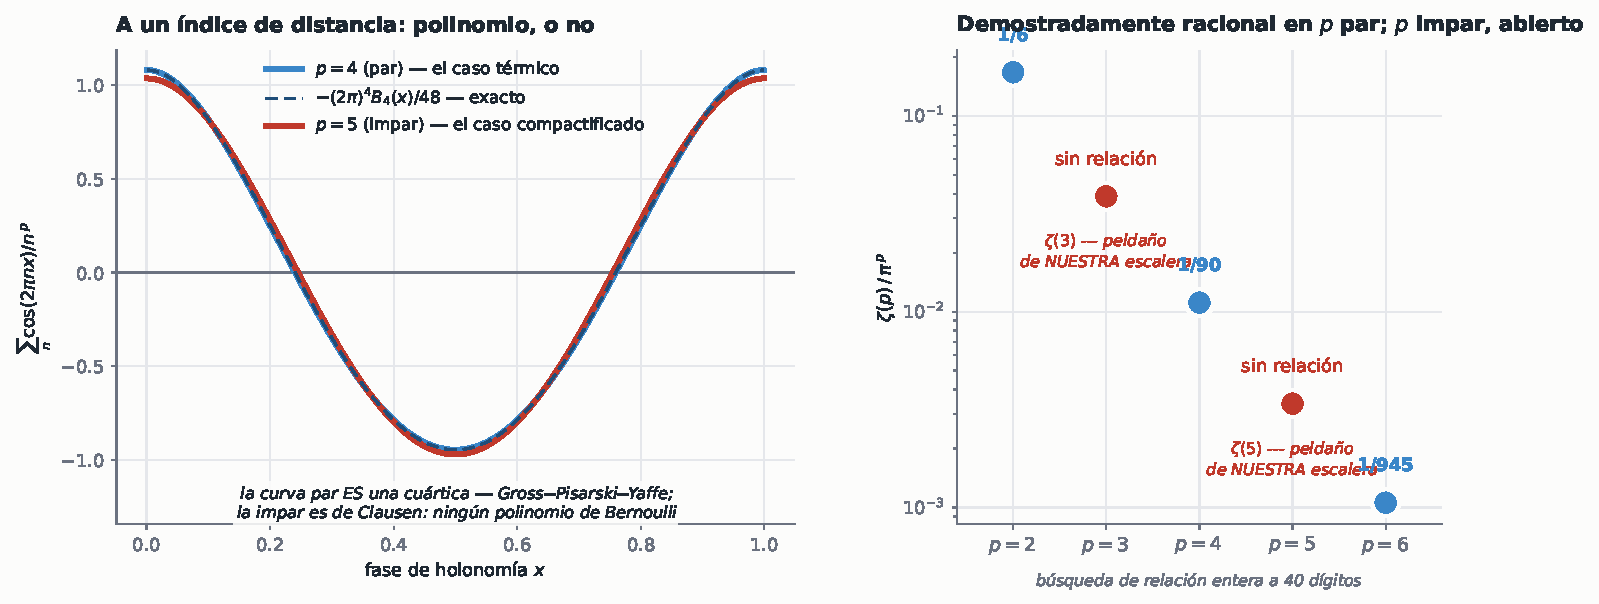
\includegraphics[width=\textwidth]{fig_parity_es.pdf}
\caption{\textbf{A un índice de distancia.} La misma suma de Fourier a exponente par y a exponente impar. En $p=4$ \emph{es} una cuártica ---la curva discontinua es $-(2\pi)^4B_4(x)/48$, el potencial de Gross-Pisarski-Yaffe, y las dos coinciden hasta $10^{-41}$. En $p=5$ no existe tal expresión. A la derecha, la señal aritmética: $\zeta(p)/\pi^p$ es racional para $p$ par, y eso es un teorema; para $p$ impar está abierto, y una búsqueda de relaciones enteras a $40$ dígitos devuelve $1/6$, $1/90$ y $1/945$ y no encuentra nada para $\zeta(3)$ ni $\zeta(5)$ ---que son los dos peldaños de nuestra escalera. Evidencia, no demostración: lo que descarta un polinomio con rigor es el punto de ramificación $x^4\ln x$.}\label{fig:parity}
\end{figure}

\bridge{Fijada la forma de la respuesta, el desarrollo mismo: una sola serie, leída peldaño a
peldaño, cada uno emparejando un momento del contenido con un valor de zeta. Tres peldaños llevan
la física, y donde iría el cuarto hay un polo ---que resulta ser el último sitio por donde puede
entrar un trascendente nuevo.}

% ===================================================================
\section{Un desarrollo, tres peldaños}\label{sec:ladder}

Desarrollar \eqref{eq:F} en la fase es una sola operación:
\begin{equation}\label{eq:expansion}
  \mathrm{Re}\,\mathrm{Li}_5\!\left(s\,e^{ic\pi\alpha}\right)
  \;=\;\sum_{k\ge0}\frac{(-1)^k (c\pi\alpha)^{2k}}{(2k)!}\;\sum_{n\ge1}\frac{s^n}{n^{5-2k}}\,,
\end{equation}
de modo que la derivada $2k$-ésima en $\alpha$ queda gobernada por $p=5-2k$ \emph{y} por el momento
$2k$-ésimo del contenido. La suma interior se parte de una vez por todas, porque $s^n=+1$ en los
enrollamientos pares sea cual sea $s$:
\begin{equation}\label{eq:split}
  \sum_{n\ge1}\frac{s^n}{n^{p}}\;=\;2^{-p}\zeta(p)\;+\;s\,(1-2^{-p})\,\zeta(p)\,.
\end{equation}
Sumados sobre el contenido, los dos corchetes recogen los dos momentos de golpe ---uno ciego a la
paridad, otro pesado por ella--- y el coeficiente del peldaño $k$ es, con la última columna de la
tabla de abajo leída sobre la semilla gauge que imprime \cite{KM25},
\begin{equation}\label{eq:rung}
  \frac{S_k+(2^{p}-1)\,\Delta_k}{2^{p}}\,,\qquad
  S_k=\sum m\,c^{2k}\,,\qquad \Delta_k=\sum m\,c^{2k}s\,.
\end{equation}

\begin{center}\small
\rowcolors{2}{white}{softgrey}
\begin{tabular}{ccll r}
\toprule
\rowcolor{hdrblue!10}$k$ & $p$ & objeto & coeficiente & sector gauge\\
\midrule
$0$ & $5$ & el \emph{valor} $F(0)$ & $(S_0+31\Delta_0)/32$ & $9$\\
\rowcolor{amber!14}$1$ & $3$ & la \emph{curvatura} $V''(0)=-\pi^2\zeta(3)D$ & $(S_1+7\Delta_1)/8$ & $-27$\\
$2$ & $1$ & el cuarto momento & $(S_2+\Delta_2)/2=\mathcal{A}_2=A_4$ --- sólo la periódica & $-36$\\
\bottomrule
\end{tabular}
\end{center}

\noindent Los octavos de la Parte~VI son $2^3$ y su siete es $2^3-1$; los denominadores $32,8,2$ son
$2^p$. En $p=1$ divergen las dos mitades de \eqref{eq:split}, y lo que se hace de ellas depende de
la paridad: en $s=-1$ se cancelan y dejan un $-\ln2$ \emph{finito}, mientras que en $s=+1$ se suman
y el polo sobrevive. \textbf{De modo que el $x^4\ln x$ es el polo sin cancelar del sector
\emph{periódico}}, y lo que aporta el antiperiódico es el $\ln2$ que la \eqref{eq:moments} lleva
sobre $B_4$. $\mathrm{Li}_5$ tiene exactamente un logaritmo en $x$, y es sólo del periodico ---que
es la fila $p=1$ de la tabla de arriba, leída como enunciado analítico y no de contabilidad.

\paragraph{La escalera es geométrica, y la carga dos es su punto fijo.} Como $2^{p}=32/4^{k}$, un
término suelto $(m,s,c)$ recorre la escalera como una sucesión geométrica:
\begin{keyeq}
\begin{equation}\label{eq:modes}
  s=+1:\;\; 32\,m\,\sigma^k \;\;\text{con}\;\;\sigma=\tfrac{c^2}{4};
  \qquad
  s=-1:\;\; 2\,m\,(c^2)^k - 32\,m\,\sigma^k \;\;\text{--- dos modos.}
\end{equation}
\end{keyeq}
Luego $O_k=\sum_\sigma A_\sigma\,\sigma^k$, con $\sigma\in\{\tfrac14,1,\tfrac94\}$ procedente de
$c=1,2,3$ y, sólo para los estados antiperiódicos, además $\sigma\in\{1,4,9\}$.

\begin{keyeq}
Un estado periódico de \emph{carga dos} tiene $\sigma=1$: pesa exactamente lo mismo en el valor, en
la curvatura y en el cuarto momento. La carga uno decae por cuatro en cada peldaño; la carga tres
crece. El sector gauge sólo alcanza $\{\tfrac14,1\}$, de modo que su escalera tiene dos parámetros
en vez de tres, y
\[
  O(5)-O(3)\;=\;4\,\bigl[\,O(3)-O(1)\,\bigr]
\]
idénticamente ---cero contraejemplos sobre las $4096$ asignaciones de paridad admisibles. Sus dos
amplitudes se calculan en la \S\ref{sec:arith}, \eqref{eq:gaugerung}, donde la identidad pasa a ser
una línea de álgebra en lugar de un recuento.
\end{keyeq}

La relación geométrica sobrevive a cualquier contenido de materia que no abra un tercer modo, y muere en cuanto
aparece uno. Predicha antes de calcular la tabla y confirmada en los ocho multipletes: vale para
$\rep7^{(\pm)}$, $\rep{28}^{(+,+)}$ y $\rep{48}^{(+,+)}$, y se rompe para $\rep{28}^{(+,-)}$ y
$\rep{48}^{(+,-)}$ ---que se diferencian de sus compañeros sólo en si su estado de carga dos es
periódico o antiperiódico--- y para los dos $\rep{84}$, los únicos multipletes que llevan una carga
tres. Toda fila de su Tabla~1 contiene un $\rep{84}$, así que para cada fila publicada el valor, la
curvatura y el cuarto momento son tres números independientes; sin él, son dos.

\paragraph{Y esa última diferencia es más afilada de lo que parece: el cambio de paridad en
carga dos es el único sin logaritmo.} Mueva una
unidad de multiplicidad de carga $c$ de la torre periódica a la antiperiódica. Los tres momentos se
desplazan en
\[
  \Delta D=-\tfrac74c^2,\qquad \Delta A_4=-c^4,\qquad
  \Delta G=-c^4\Bigl(H_4-\ln\tfrac{c}{2}\Bigr),
\]
y $\Delta G$ es \emph{racional} exactamente cuando $c=2$, porque entonces $\ln c$ es el mismo $\ln2$
que la torre antiperiódica lleva de forma universal en \eqref{eq:moments}. Así que en carga dos, y en
ninguna otra, el cambio de paridad no lleva logaritmos, con la firma exacta
\begin{equation}\label{eq:c2flip}
  (\Delta D,\;\Delta A_4,\;\Delta G)\;=\;\bigl(-7,\;-16,\;-\tfrac{100}{3}\bigr)\ \text{por unidad,}
\end{equation}
y, de forma equivalente, $J\equiv G-H_4A_4=-A_4^{L}-\ln2\,B_4$ es completamente ciego a la paridad
de un estado de carga dos. Que ésta sea la misma carga que se sienta en el punto fijo de
\eqref{eq:modes} no es consecuencia de aquello: $\sigma=1$ habla de $c^2/4$ y esto habla de
$\ln(c/2)$, y las dos coinciden sólo porque ambas piden que $c$ valga $2$.

Sugirió una prueba sobre el residuo del anclaje de la Parte~VI, ya que las filas que fallan son las
que contienen un $\rep{48}$ y la paridad de un estado de carga dos es lo que distingue
$\rep{28}^{(+,+)}$ de $\rep{28}^{(+,-)}$ y $\rep{48}^{(+,+)}$ de $\rep{48}^{(+,-)}$: si el residuo
fuera una paridad de carga dos mal leída, su $(\amin,m_h)$ publicado se sentaría en nuestros momentos
desplazados un múltiplo entero de \eqref{eq:c2flip}. Despejar ese múltiplo de (II) y comprobar luego
(I), que el despeje no ha visto, da múltiplos no enteros entre $0.03$ y $0.15$ y residuos en (I) del
orden de $10^{-1}$ a $1$; dos vectores señuelo, los cambios en $c=1$ y $c=3$ que sí llevan
logaritmo, no lo hacen peor. \textbf{La prueba sale negativa y la lectura se retira}: sea lo que sea
el residuo del anclaje, no es una paridad de carga dos. Queda anotado porque el vector es exacto y
barato de volver a probar contra cualquier candidato futuro.

Pero la propiedad de no llevar logaritmo sobrevive a la prueba para la que se inventó, y no es un
accidente de que $c=2$ sea pequeño. La \S\ref{sec:ceiling} escribe $G$ en la base
$\{1,\ln2,\ln3\}$ y encuentra el contenido sentado en un retículo de \emph{cuatro} dimensiones
cuyas coordenadas logarítmicas son los pesos de $\ln2$ y de $\ln3$, $U$ y $V$. En ese retículo el
cambio de paridad en carga dos es el movimiento con $\Delta U=\Delta V=0$ ---la única dirección de
generador que el tercer eje no ve--- y \emph{por eso} su $\Delta G$ salía racional: sin logaritmo
que se mueva, $\Delta G$ sólo puede valer $\tfrac{25}{12}\Delta A_4$, que es $-\tfrac{100}{3}$.
Medido en \texttt{crossed\_\allowbreak equations.py} y \texttt{semigroup.py}.

\paragraph{El peldaño de arriba no es nuestro, y tampoco lo es menos de lo que le sacamos al
principio.} Cacciapaglia \emph{et al.}~\cite{CCD24} deciden la estabilidad del orbifold comparando
el potencial en $a=0$ y en $a=1/2$, y sus ecs.~(2.11)--(2.13) dan $F_-(0)=-\tfrac{15}{16}F_+(0)$,
con $\tfrac{15}{16}=\eta(5)/\zeta(5)$, y el signo decidiendo si el orbifold es estable ---un peso ya
impreso en \cite{PP01} ec.~(13) en 2001, como
$V^{-,\text{escalar}}=-\tfrac{15}{16}V^{+,\text{escalar}}$. El \emph{reparto} del que sale está
también en seis dimensiones, en \cite{GHBQ05} ec.~(3.18), donde las dos paridades del orbifold
entran como $\mathrm{Li}_n(\pm q)$ ---pero el peso no: ese artículo nunca evalúa el cociente, y las
cadenas $15/16$, $31/32$ y $\zeta(5)$ no aparecen en ninguna de sus cuarenta páginas. \textbf{La
arquitectura del reparto por paridad es suya y aquí no se reclama.} Y su ec.~(2.11) dice más que ese
valor: $F_-(a)=-F_+(a)+\tfrac1{16}F_+(2a)$ es una identidad en $a$ ---la fórmula de duplicación
\cite{Wood}, no la \eqref{eq:split} en un punto--- y la \S\ref{sec:closed} la usa como tal. Leída
sólo en $a=0$ es el peldaño de arriba; leída como función es la razón de que el potencial genere
cinco. Lo que su método no alcanza es
la curvatura: en $45$ páginas no aparecen las palabras \emph{curvatura} ni \emph{segunda derivada},
ni \emph{Dynkin} ni \emph{traza}, y su única segunda derivada (su ec.~(3.15)) se toma en un ejemplo
donde el potencial ya ha colapsado a un solo término, de modo que en ella no aparece ningún reparto
por paridad. Su propio texto dice por qué no van por ahí: los valores esperados de vacío pequeños,
escriben, ``se obtienen normalmente mediante alguna forma de ajuste fino'' ---y el mínimo interior a
$\alpha$ pequeño que dejan de lado es precisamente el régimen de \cite{KM25} y de este artículo. La
\S\ref{sec:novel} enuncia la frontera al completo.

\textbf{Su criterio de estabilidad también es suyo}, y reaparece en la \S\ref{sec:ceiling}: comparar
el potencial en los dos puntos simétricos es lo que decide si el mínimo a $\alpha$ pequeño que aquí
se calcula es el vacío o solamente un vacío, y \cite{CCD24} lo enuncian, demuestran las identidades
que necesita y sacan su regla de signos. La \eqref{eq:truevac} es ese enunciado sumado sobre un
contenido de bulk, en nuestra notación y sin añadir nada. Lo único nuestro es el uso: sumado resulta
\emph{lineal} en las multiplicidades, así que cabe dentro del programa entero que produce el techo,
y por eso el techo se calcula dos veces, llevándose las dos respuestas $0.8$~TeV.
La Figura~\ref{fig:ladder} es la estructura de
peldaños que añade la curvatura, con los tres peldaños propios del sector gauge al lado.

\begin{figure}[t]\centering
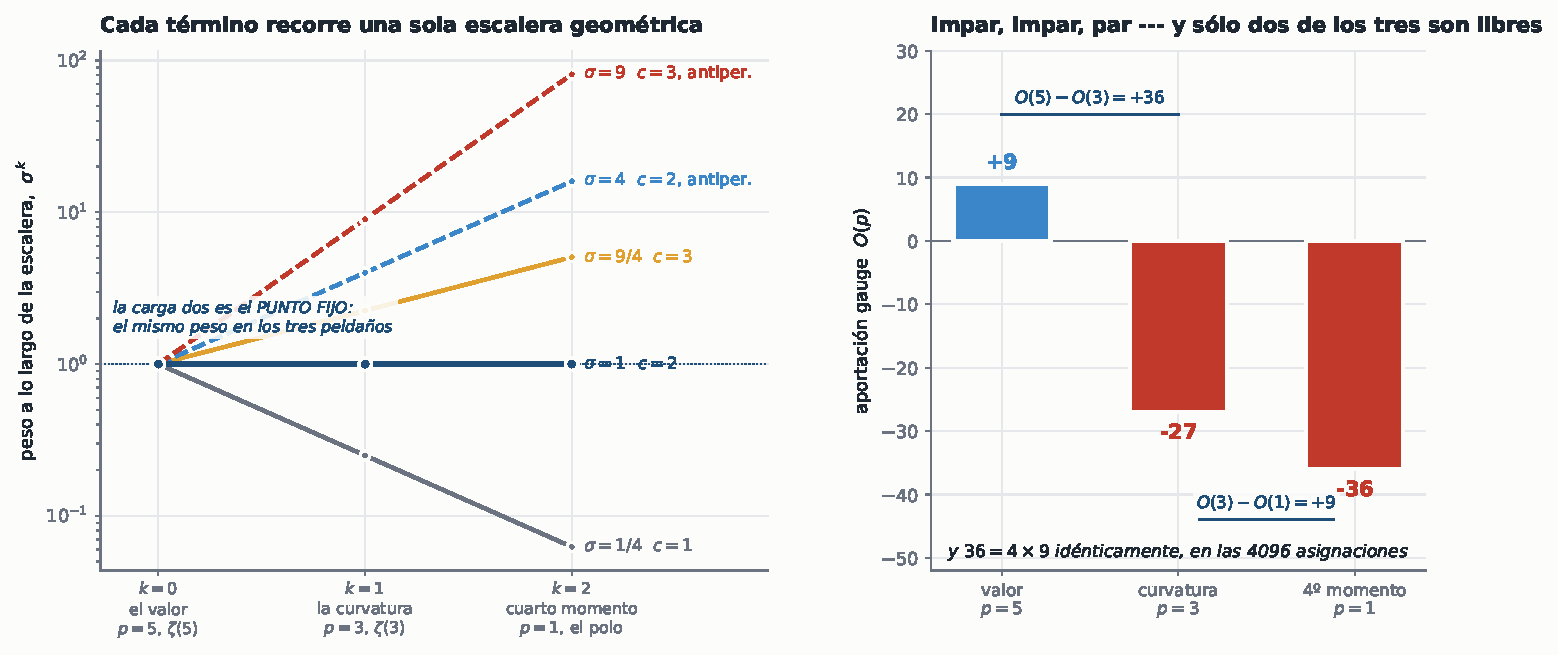
\includegraphics[width=\textwidth]{fig_ladder_es.pdf}
\caption{\textbf{La escalera es geométrica.} A la izquierda: cada término del potencial recorre los tres peldaños como $\sigma^k$ con $\sigma=c^2/4$, y los términos antiperiódicos llevan un segundo modo $\sigma=c^2$. Un estado periódico de carga dos tiene $\sigma=1$: pesa lo mismo en el valor, en la curvatura y en el cuarto momento, y es el espinazo plano del que todo lo demás se abre en abanico. A la derecha, los tres peldaños propios del sector gauge con la semilla que \cite{KM25} imprimen: impar, impar y par. Sólo alcanza $\sigma\in\{1/4,1\}$, así que dos de los tres números determinan el tercero ---en cada una de las $4096$ asignaciones de paridad admisibles.}\label{fig:ladder}
\end{figure}

\bridge{El peldaño de la curvatura es donde se decide el vacío, así que ése es el peldaño que hay
que resolver.}

% ===================================================================
\section{La jerarquía en forma cerrada}\label{sec:closed}

Conservando los tres peldaños de la \S\ref{sec:ladder} y escribiendo $x=\pi\alpha$,
\begin{equation}\label{eq:Fexp}
  F(x)\;=\;\text{const}\;-\;\frac{\zeta(3)D}{2}\,x^2\;+\;\frac{x^4}{24}\bigl[\,G-A_4\ln x\,\bigr]
  \;+\;O(x^6)\,,
\end{equation}
siendo el logaritmo el peldaño $p=1$. El punto simétrico es por tanto \emph{estacionario pero no
analítico}: $x^4\ln x$ y sus dos primeras derivadas se anulan en el origen, de modo que $F'(0)=0$ y
$F''(0)=-\zeta(3)D$ están perfectamente definidas ---que es lo que autoriza al
Teorema~\ref{thm:eighths} a hablar siquiera de la curvatura de ahí---, mientras que el punto de
ramificación vive dos derivadas más arriba y no existe serie de Taylor ordinaria. Y
$\mathrm{d}F/\mathrm{d}x=0$ da, en lugar de la raíz
de un polinomio,
\begin{keyeq}
\begin{equation}\label{eq:amin}
  x^2 \;=\; \frac{24\,\zeta(3)\,D}{\,4G - A_4\,(4\ln x + 1)\,}\,,\qquad x=\pi\amin .
\end{equation}
\end{keyeq}

\noindent La jerarquía es un cociente de dos momentos del contenido, corregido por un tercero.

\paragraph{Y es una forma cerrada, que veníamos llamando punto fijo.} Las versiones anteriores
resolvían la \eqref{eq:amin} por iteración y la llamaban ecuación de punto fijo en vez de
resoluble. Es resoluble. Con $y=x^2$, de modo que $\ln x=\tfrac12\ln y$, queda $y\,(b-\ln y)=d$ con
$b=(4G-A_4)/(2A_4)$ y $d=12\zeta(3)D/A_4$; y con $u=\ln y-b$ eso es $u\,e^{u}=-d\,e^{-b}$, la
definición misma de la función $W$ de Lambert. Por tanto
\begin{keyeq}
\begin{equation}\label{eq:lambert}
  x^{2}\;=\;\frac{-d}{W\!\left(-d\,e^{-b}\right)}\,,\qquad
  b=\frac{4G-A_4}{2A_4}\,,\qquad d=\frac{12\,\zeta(3)\,D}{A_4}\,.
\end{equation}
\end{keyeq}
Que el argumento sea negativo es necesario para tener dos ramas reales, pero no suficiente: $W$ es
real sólo si $z\ge-1/e$, que aquí se lee $b-1-\ln d\ge0$. Esa condición se cumple en todo contenido
de los usados aquí, y no es una hipótesis añadida. \textbf{Cuál de las dos ramas es el mínimo no es una
etiqueta sino un teorema}, y de una línea: eliminar $x^2$ entre la \eqref{eq:lambert} y la
identidad~(II) de la \eqref{eq:two} da
\begin{equation}\label{eq:branchmu}
  \mu\;=\;-\frac{A_4}{6}\,(W+1)\,,\qquad\text{equivalentemente}\qquad W_{-1}=-1-\frac{6\mu}{A_4}\,,
\end{equation}
con $\mu=m_h^2/(K\pi^2)^2$. Como $A_4>0$, la rama con $W\le-1$ lleva $\mu\ge0$ y la rama con
$-1<W<0$ lleva $\mu<0$: \emph{el signo de la masa del Higgs al cuadrado es el signo de $-(W+1)$}.
Así que $W_{-1}$ es el mínimo y $W_{0}$ un máximo, demostrado y no asignado; en las cinco filas
publicadas $\mu$ va de $81$ a $115$ en la primera y de $-30$ a $-38$ en la segunda. Dice además
que la masa del Higgs medida \emph{selecciona un punto de la hoja de Lambert}, y que $m_h\to0$ es
$W\to-1$ ---el punto de ramificación, que es el pliegue que el Teorema~\ref{thm:eighths} tiene
cuidado de no reclamar---. Verificado en \texttt{lambert\_\allowbreak criticality.py}. \textbf{Ninguna de las dos es uno
de los dos puntos simétricos $\alpha=0,1$ que compara la \S\ref{sec:ceiling}}: aquéllos son
extremos del dominio, su diferencia \eqref{eq:truevac} se evalúa de forma exacta y no a través de
este desarrollo, y la raíz exterior no interviene en el techo. Comprobado
contra la iteración en las cinco filas publicadas hasta $1.8\times10^{-14}$, en
\texttt{lambert\_\allowbreak amin.py}. Corrige además una pieza de nuestro relato: la
\S\ref{sec:parity} descarta un \emph{polinomio}, cosa que el punto de ramificación hace con rigor,
y eso es todo lo que descarta ---nunca una forma cerrada. La misma $W$ ya estaba una sección más
adelante, en la \eqref{eq:rinf}, antes de reconocer la ecuación a la que pertenece.

\paragraph{Y en las coordenadas adecuadas toda la familia es una sola imagen.} Póngase
$L=b-1-\ln d$, el discriminante mismo ---hay dos ramas reales exactamente cuando $L\ge0$---.
Entonces $b=L+1+\ln d$ y el argumento de la función de Lambert pierde su segundo parámetro de
golpe, $z=-d\,e^{-b}=-e^{-(1+L)}$, de modo que la \eqref{eq:lambert} se separa:
\begin{equation}\label{eq:foldsep}
  x^{2}\;=\;d\;f(L),\qquad f(L)=\frac{-1}{W\!\left(-e^{-(1+L)}\right)}\,,
\end{equation}
un factor por coordenada. Las dos ramas son entonces dos hojas de una misma superficie sobre
$(L,d)$, y se juntan donde $W=-1$, es decir $f=1$, es decir el borde \emph{recto} $L=0$ ---a lo
largo de todo el cual $\mu=0$, por la \eqref{eq:branchmu}. \textbf{La forma cerrada es la hoja de
arriba de un pliegue, y la masa del Higgs es la altura sobre su borde.} La
Figura~\ref{fig:lambert} es esa superficie, con sus cinco filas publicadas y el vértice donde se
alcanza el techo de la \S\ref{sec:ceiling} de pie encima.

\begin{figure}[t]
\centering
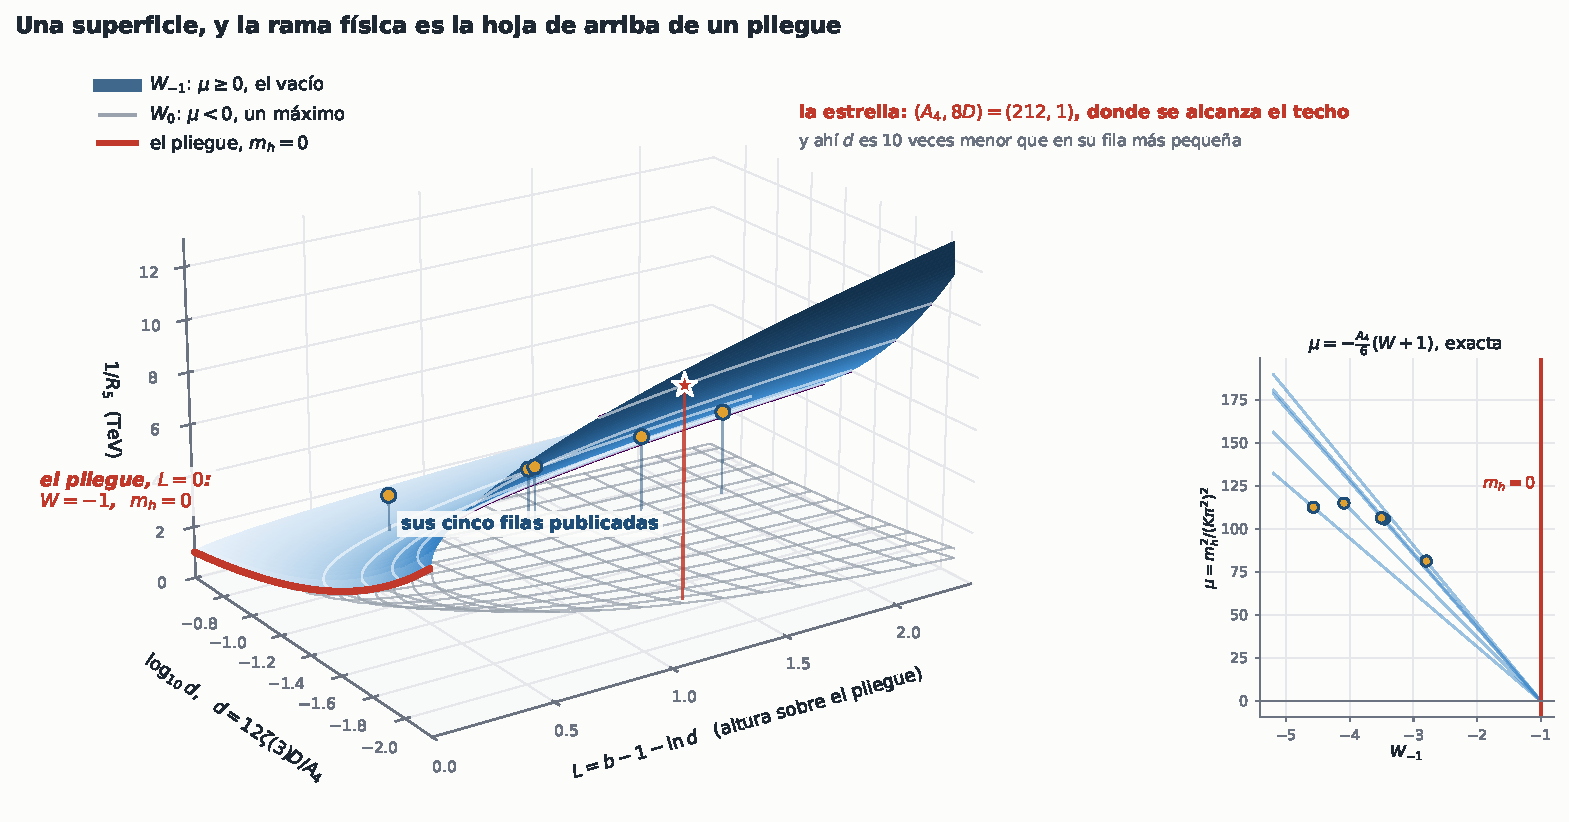
\includegraphics[width=\textwidth]{fig_lambert_es.pdf}
\caption{\textbf{La forma cerrada es una hoja de un pliegue.} $1/R_5=2\pi m_W/x$ sobre las dos
coordenadas de la \eqref{eq:foldsep}: $L=b-1-\ln d$, el discriminante, y $d=12\zeta(3)D/A_4$, en eje
logarítmico porque el vértice del certificado y sus filas publicadas difieren en él en un factor
diez. La hoja azul es $W_{-1}$, donde $\mu\ge0$ y el punto estacionario es el vacío; la malla gris
abierta de debajo es $W_0$, donde $\mu<0$ y ese mismo punto es un máximo. Se juntan a lo largo del
borde rojo $L=0$, donde $W=-1$ y por tanto $m_h=0$: éste es el punto de ramificación \emph{de
Lambert}, donde el mínimo electrodébil y la raíz exterior se funden, y no el de $\alpha^4\ln\alpha$
en el origen sobre el que gira la \S\ref{sec:parity} ---es el pliegue que el
Teorema~\ref{thm:eighths} tiene cuidado de no reclamar, dibujado y no descrito. Los discos ámbar son las cinco filas de
\cite{KM25}; la estrella es $(A_4,8D)=(212,1)$, el vértice donde se alcanza el techo. \textbf{La
estrella no está en $10.03$~TeV, y no debe estarlo}: la superficie devuelve el punto estacionario
\emph{propio} de cada contenido, ahí $9967$~GeV, mientras que el certificado lee la
\eqref{eq:two}(II) en el techo de la ventana de Higgs ---una diferencia del $0.7\%$, y toda ella es
qué $m_h$ se está pidiendo. \emph{Recuadro:} la \eqref{eq:branchmu} como la recta que es, una por
fila, las cinco encontrándose en $W=-1$, $\mu=0$. Dibujada por
\texttt{make\_\allowbreak fig\_\allowbreak lambert.py}, que se niega a dibujar si la superficie no
devuelve cada $\amin$ representado ---lo hace, a $2\times10^{-14}$.}\label{fig:lambert}
\end{figure}

\paragraph{Verificación, contra nuestra propia minimización y no contra su columna.} Lo que aquí se
pone a prueba es el desarrollo, no el anclaje: un desacuerdo sería un defecto de \eqref{eq:amin} y
de nada más. Sobre $272$ contenidos sintéticos que abarcan doce valores de $D$ y
$\amin\in[0.018,0.119]$ ---el rango de su Tabla~1--- el error mediano es del $0.13\%$, y del
$0.004\%$ en el extremo de $\alpha$ pequeño, donde la cola truncada es menor. Sobre las
cinco filas publicadas:

\begin{center}\small
\rowcolors{2}{white}{softgrey}
\begin{tabular}{lrrrrr}
\toprule
\rowcolor{hdrblue!10}fila & $D$ & $A_4$ & $\amin$ numérico & forma cerrada & error\\
\midrule
(1) & $15/8$ & $258$ & $0.055304$ & $0.055423$ & $0.215\%$\\
\rowcolor{amber!12}(2) & $29/8$ & $271$ & $0.083062$ & $0.083579$ & $0.623\%$\\
(3) & $9/8$  & $189$ & $0.043593$ & $0.043621$ & $0.065\%$\\
(4) & $11/8$ & $223$ & $0.046879$ & $0.046929$ & $0.107\%$\\
(5) & $15/8$ & $255$ & $0.055277$ & $0.055393$ & $0.209\%$\\
\bottomrule
\end{tabular}
\end{center}

\noindent Mediana $0.209\%$, máximo $0.623\%$ ---y el máximo cae en la fila de $\alpha$ mayor, que es
donde la cola truncada es mayor. Los dos quedan holgadamente dentro de las
dos cifras significativas con las que está impresa esa tabla.

Tres controles corren en paralelo, y el último es el que podía haber fallado. La columna $D$ sale en
octavos exactos. Se reproduce el patrón de cocientes publicado en la Parte~VI \S7: $1.939$ en las
dos filas con un $\rep{48}$ frente a $1.199$ en las otras tres. Y \emph{quitar el logaritmo} ---usar
$x^2=24\zeta(3)D/4G$, que es lo que uno escribiría sin la \S\ref{sec:parity}--- falla entre un $+104$
y un $+174\%$. El punto de ramificación no es un adorno.

\paragraph{Y el truncamiento es una cola, no una estimación asintótica ---lo que dice más de lo
que parece, y es lo que la \S\ref{sec:ceiling} va a necesitar.} La escalera no se detiene en $p=1$. Su índice sigue a $p=-1,-3,-5,\dots$, donde $\zeta$ es
\emph{racional} por Bernoulli, así que pasado su propio polo el desarrollo no genera ningún
trascendente nuevo: el peldaño de orden $x^{2k}$ es $\zeta(5-2k)\,[\,A_{2k}+(2^{2k-4}-1)B_{2k}\,]$,
que es \eqref{eq:ladderab} leída a $p$ negativo, y el peso antiperiódico corre
$3,\,15,\,63,\,255,\dots=2^{2k-4}-1$. \textbf{Hay exactamente un logaritmo en todo el desarrollo},
a orden $x^4$, y todo término posterior es racional en los momentos; el contenido trascendente del
potencial es $\zeta(5)$, $\zeta(3)$, $\ln x$, $\ln 2$ y $\ln 3$, y nada más. Éste es el desarrollo
clásico de $\mathrm{Li}_n(e^{\mu})$ en torno a $\mu=0$ \cite{Lewin}, válido para $|\mu|<2\pi$, y su
término $H_{n-1}-\ln(-\mu)$ en $n=5$ es el $H_4=\tfrac{25}{12}$ que $G$ ya lleva en
\eqref{eq:moments} ---la misma constante, llegando por una segunda vía. Extraído ese único
logaritmo, el resto es por tanto la cola de una serie \emph{convergente}, con radio fijado por la
singularidad más próxima de $\mathrm{Li}_5(s\,e^{ic\pi\alpha})$, en $s\,e^{ic\pi\alpha}=1$:
$\alpha=2n/c$ para la torre periódica y $\alpha=(2n+1)/c$ para la antiperiódica, de modo que
$|\alpha|<1/c_{\max}=1/3$ cubre las dos. Medido término a término, la razón asintótica es
$(c\alpha)^2$ antiperiódica y $(c\alpha/2)^2$ periódica, con controles a los dos lados de los dos
radios ---la serie converge en $\alpha=0.32$ y diverge en $\alpha=0.40$ para la torre
antiperiódica, y converge en $\alpha=0.40$ y diverge en $\alpha=0.70$ para la periódica---. Todo
$\alpha$ que usa este artículo queda dentro de $1/3$ por un factor de al menos $2.7$. \textbf{Así
que el error cometido aquí es un resto convergente y admite una cota rigurosa en vez de una
estimación}, que es lo que suministra la cota compañera de
\texttt{remainder\_\allowbreak theorem.py}. Medido en \texttt{crossed\_\allowbreak equations.py}.

Que el contenido trascendente sea exactamente $\{\zeta(5),\zeta(3),\ln x,\ln 2,\ln 3\}$ no es una
curiosidad de paso; es un sistema de coordenadas, y la \S\ref{sec:ceiling} lo gasta. Como los
únicos logaritmos de \emph{números} son $\ln2$ y $\ln3$ ---las cargas llegan a tres y no más---,
el momento $G$ se descompone exactamente en la base $\{1,\ln2,\ln3\}$, que es lo que convierte la
condición trascendente que decide el techo en un programa entero. Los dos enunciados son uno solo,
leído en dos peldaños de la misma escalera.

\bridge{El mismo desarrollo tiene una segunda salida, y es la columna que uno no espera que salga
gratis.}

% ===================================================================
\section{La masa del Higgs, de los mismos dos momentos}\label{sec:mh}

Derivar \eqref{eq:Fexp} dos veces y usar la condición de estacionariedad para eliminar
$G-A_4\ln x$ produce una cancelación que conviene aislar:
\begin{keyeq}
\begin{equation}\label{eq:fpp}
  F''(\amin)\;=\;\pi^2\Bigl[\,2\zeta(3)D-\tfrac16 A_4 x^2\,\Bigr]\,.
\end{equation}
\textbf{El logaritmo y $G$ se cancelan idénticamente en el punto estacionario.}
\end{keyeq}

\noindent Con su ec.~(80), $m_h=K\sqrt{F''(\amin)}/\amin$ y $K=(\sqrt3/2\pi^3)m_W g_4$, las dos
columnas de su Tabla~1 son funciones de $(D,A_4)$ y de nada más, sin minimización por ninguna
parte ---funciones que devuelven \emph{nuestros} valores de las dos, porque por la
\S\ref{sec:setting} el de $\amin$ no reproduce el suyo.
Frente a una segunda derivada numérica del mismo potencial, la forma cerrada concuerda entre el
$0.13$ y el $1.22\%$ a lo largo de las cinco filas, y el $m_h$ resultante entre el $0.07$ y el
$0.61\%$.

Un control que tiene que dispararse, y se dispara: su ec.~(80) no devuelve ningún $m_h$ real donde
$F''<0$, y en \emph{su} $\alpha$ publicado de la fila~(3) nuestro ensamblaje da $F''=-2.45$. Es un
síntoma de la discrepancia de anclaje de la \S\ref{sec:setting}, registrada en la Parte~VI y no
resuelta aquí.

\bridge{Los dos observables salen ya de dos enteros disfrazados. La pregunta siguiente es qué se les
permite ser a esos enteros.}

% ===================================================================
\section{La aritmética del contenido}\label{sec:arith}

En la base suma/diferencia $S=A_2+B_2$, $\Delta=A_2-B_2$, el peldaño de la curvatura se lee
$8D=S+7\Delta$, y el siete es $2^3-1$ del cociente de zetas, no de $\su7$.

\paragraph{Y no es una coincidencia de notación: $D$ \emph{es} un peldaño.} Escribiendo el peldaño
de la \S\ref{sec:ladder} como $O_k=[S_k+(2^p-1)\Delta_k]/2^p$ con $p=5-2k$ y leyéndolo en los dos
valores de $k$ que este artículo usa,
\[
  k=1:\quad O_1=\frac{S+7\Delta}{8}=D,
  \qquad\qquad
  k=0:\quad O_0=\frac{S_0+31\Delta_0}{32},\quad F(0)=\zeta(5)\,O_0 .
\]
Así que el invariante de curvatura de esta sección y el criterio de estabilidad de \cite{CCD24} son
el mismo objeto evaluado en dos peldaños de una misma escalera, y el $7$ y el $31$ son $2^p-1$ en
cada uno. Los octavos impares del Teorema~\ref{thm:eighths} y la cota $|F(0)|\ge\zeta(5)/32$ son
entonces un solo enunciado leído dos veces, y por eso los numeradores del sector gauge $9$, $-27$,
$-36$ en $k=0,1,2$ son impar, impar, par \emph{con la semilla que \cite{KM25} imprimen}: la
obstrucción está viva en el valor y en la curvatura y
muere en el cuarto momento, donde $p=1$, la mitad antiperiódica se cancela en un $\ln2$ finito y el
polo periódico sobrevive como el $x^4\ln x$. Con la semilla candidata de la \S\ref{sec:open} esos mismos tres
numeradores son $18$, $-18$, $-27$, y el patrón \emph{se permuta} a par, par, impar. Lo que se
anula en $p=1$ es la mitad antiperiódica, no la obstrucción: deja al peso \emph{periódico} solo
llevando la paridad, y ese peso es justo el que decide la bifurcación de la \S\ref{sec:open}.
\textbf{Leída de una vez en los tres peldaños, la escalera es una \emph{tomografía} de la semilla
gauge}: en $p=5$ y $p=3$ el carácter de paridad lee los dos sectores $P_6$ combinados, y en $p=1$,
donde $2-2^{p}$ se anula, lee el sector periódico solo. De modo que mover la semilla no apaga la
protección: la traslada al peldaño que lee la mitad que la semilla cambió.

\begin{theorem}[los octavos impares, condicionado]\label{thm:eighths}
\emph{Si} la contribución del sector gauge a $8D$ es impar, entonces $8D$ es un entero impar para
todo contenido de bulk. Por tanto $D\neq0$ y $|D|\ge\tfrac18$: \emph{el punto simétrico} nunca es
marginal a un lazo, y por una cantidad cuantizada.
\end{theorem}
\begin{keyeq}
\begin{equation}\label{eq:oddeighths}
  8D_{\mathrm{gauge}}\ \text{impar}
  \quad\Longrightarrow\quad 8D\in2\ZZ+1
  \quad\Longrightarrow\quad |D|\ \ge\ \tfrac18
\end{equation}
\end{keyeq}

\begin{corollary}[para la semilla impresa en \cite{KM25}]\label{cor:kmseed}
Los coeficientes gauge de la ec.~(68) de \cite{KM25} dan $8D_{\mathrm{gauge}}=-27$, que es impar.
La hipótesis del Teorema~\ref{thm:eighths} se cumple, por tanto, y todas las consecuencias que de
él se extraen más abajo valen en este modelo.
\end{corollary}

\noindent \textbf{Por qué la hipótesis va aparte, y no es una formalidad.} La demostración necesita
dos cosas: que la materia aporte una cantidad par y que el sector gauge aporte una impar. La
primera es aritmética y no puede fallar. La segunda no se calcula aquí ---se lee de la ecuación de
otro, y la \S\ref{sec:open} muestra que esa lectura está en cuestión---. Separarla no cuesta nada,
porque el Corolario~\ref{cor:kmseed} restituye literalmente todas las consecuencias para la semilla
publicada. Lo que gana es la distinción que importa: \emph{si la semilla se mueve, el teorema sigue
siendo cierto y su hipótesis deja de cumplirse}, que es una situación distinta por completo de un
teorema que falla. Y un enunciado condicional dice algo que el incondicional no puede: exactamente qué número de aguas abajo depende de qué dato de aguas arriba.

\noindent \textbf{Y sólo el punto simétrico.} $D$ es el coeficiente de $\alpha^2$ en $\alpha=0$, así
que lo que queda separado de cero es la curvatura allí. Si el vacío \emph{roto} puede ser marginal
---$F''(\alpha_\star)=0$ con $\alpha_\star\neq0$--- es otra condición, y $D\neq0$ no la toca. En la
forma cerrada de la \S\ref{sec:closed} es el pliegue de Lambert $W=-1$, equivalentemente $m_h=0$;
queda en un $\alpha$ varias veces mayor que cualquiera de los usados aquí, donde el error del
desarrollo crece con el cuadrado de esa razón y donde, siendo un pliegue una coalescencia de
raíces, la posición no la controla un truncamiento en ningún caso. Este artículo por tanto ni lo
afirma ni lo excluye. Medido en \texttt{lambert\_\allowbreak criticality.py}.
\begin{proof}
Para la materia, $c$ y $m$ son enteros, luego $S+\Delta=2A_2$ es par y $S+7\Delta=(S+\Delta)+6\Delta$
es par ---para \emph{todo} contenido, sin referencia alguna al sector gauge---. Por hipótesis el
sector gauge aporta una cantidad impar. Par más impar es impar. Para el
Corolario~\ref{cor:kmseed}, los coeficientes de la ec.~(68) de \cite{KM25} dan $S+7\Delta=-27$.
\end{proof}

\noindent La obstrucción vive en la única fila de la tabla gauge que mezcla los dos sectores $P_6$
---el $-\tfrac72$ de la entrada con $P_6=-1$, reconstruido a partir de sus ecs.~(63)--(67) y no
derivado de la geometría (\S\ref{sec:open})---. \textbf{Y lo que carga con la paridad es el
coeficiente entero de esa fila, no ninguno de los pesos que lleva dentro.} Escrita sobre sus
$n_+=2$ pares periódicos y $n_-=6$ antiperiódicos, la fila vale $2a+6b$, que con la semilla que
\cite{KM25} imprimen es $2\times2+6\times\tfrac12=7$. El $\tfrac12$ por par no lo hace él solo:
$6\times\tfrac12=3$ es \emph{entero}. Lo impar es la \emph{suma}, y eso necesita que la parte
periódica sea par tanto como que la antiperiódica sea impar ---que es el carácter de paridad
\eqref{eq:chigauge} del punto base gauge afín, y la \S\ref{sec:open} es donde eso pasa a ser el
objeto del que depende la bifurcación entera. Un recuento sobre las $4096$ asignaciones
diagonales de paridad admisibles da el mismo enunciado en forma de teoría de grupos: $D$ no puede
anularse nunca exactamente cuando el bloque que las dos proyecciones dejan sin romper tiene
dimensión impar, y en su asignación ese bloque es $\su3_C$. \emph{Con la semilla que imprime
\cite{KM25}, $D\neq0$ porque el número de colores es impar} ---y esa lectura es una propiedad de
los pesos $(2,\tfrac12)$, no del grupo: con $(\tfrac32,\tfrac12)$ los tres colores siguen ahí, el
recuento devuelve lo mismo, y $8D$ sale par igualmente (\S\ref{sec:open})---. Dentro de la clase pentadimensional
que cubre la fórmula de \cite{HY04} ---$\su{N}$ sobre $S^1/\ZZ_2$ con una sola fase de Wilson--- no
hay ningún peldaño impar; la segunda paridad independiente de este orbifold producto es la que
aporta el carácter afín de más que \emph{puede} hacer impar uno. En qué paridad cae luego el punto
base lo dice la \eqref{eq:chigauge}.

\paragraph{El teorema tiene una dimensión, y la razón obvia no es la buena.} En el rincón de paridad
única de la \S\ref{sec:anchor} toda torre tiene modos enteros, $B=0$, y $8D=8A_2$ es par; sería
fácil pararse ahí. Pero un modelo pentadimensional en $S^1/\ZZ_2$ no tiene por qué estar en ese
rincón ---con un sector antiperiódico, $B\neq0$--- y también allí $8D$ es par, de modo que no es
$B=0$ lo que hace el trabajo. Pasar la fórmula pentadimensional general de Haba y Yamashita
\cite{HY04} por todas las condiciones de contorno de $\su{N}$ en $S^1/Z_2$ que llevan una sola fase
de Wilson, hasta $N=12$, no devuelve ningún $8D$ impar. El mecanismo es el recuento de grados de
libertad: un fermión de Dirac entra con $4$ y un escalar complejo con $-2$, los dos pares, y el
único coeficiente impar ---el $-3$ del sector gauge y de fantasmas--- multiplica sólo al adjunto,
cuyo peso llega a $8D$ como $-24(2+\delta_1)+18\delta_2$, con $\delta_1,\delta_2$ los restos de
bloque de su ec.~(5.9). Aquí, en cambio, el sector gauge entrega el semientero $-\tfrac72$ de su
ec.~(68), y $6\times\tfrac72=21$ es impar. En el propio ejemplo $\su3$ de Haba y Yamashita bastan
tres multipletes para perder la protección: un fermión de Dirac adjunto con $\eta\eta'=+$ y dos
fundamentales con $\eta\eta'=-$ dan $A_2=3$, $B_2=4$ y $8D=0$ exactamente. La marginalidad no es un
rincón de ajuste fino en cinco dimensiones; es lo corriente. Lo que la prohíbe aquí es la sexta
dimensión \emph{junto con la semilla gauge} que \cite{KM25} imprimen: la candidata de la
\S\ref{sec:open} es igual de hexadimensional, tiene los mismos tres colores, y alcanza $8D=0$ en el
retículo. La segunda paridad aporta el carácter afín de más; en qué coset cae después el
desplazamiento es otra
pregunta, y es la que está abierta.

\begin{theorem}[una congruencia módulo seis]\label{thm:mod6}
Para todo contenido de bulk, $8D\equiv 2A_4+3 \pmod 6$.
\end{theorem}
\begin{keyeq}
\begin{equation}\label{eq:mod6law}
  8D\;\equiv\;2A_4+3 \pmod 6\qquad
  \text{\small para todo contenido, y con \emph{cualquiera} de las dos semillas}
\end{equation}
\end{keyeq}
\begin{proof}
Se trabaja con la combinación única $8D-2A_4$, separando el contenido del sector gauge, que entra
sólo como punto base fijo. \emph{Materia:} un estado con $s=-1$ aporta $-6mc^2$ a $8D$ y nada a
$A_4$, de modo que $8D-2A_4$ recibe $-6mc^2\equiv0\pmod6$; uno con $s=+1$ aporta $8mc^2$ y $mc^4$,
luego recibe $8mc^2-2mc^4=2mc^2(4-c^2)$, que es par, y divisible por tres porque $c^4\equiv
c^2\pmod3$ para todo entero $c$. Así que todo multiplete del bulk cumple $8D-2A_4\equiv0\pmod 6$, y
los ocho generadores lo confirman uno a uno. \emph{Gauge:} los coeficientes que \cite{KM25}
imprimen dan $8D-2A_4=-27-2(-18)=9\equiv3\pmod6$. Sumando los dos, $8D-2A_4\equiv3\pmod 6$ para
todo contenido.
\end{proof}

\noindent \textbf{Nótese que la demostración no menciona ninguna paridad, y eso no es una
preferencia de estilo.} Una versión anterior cerraba con «módulo dos, el enunciado es el
Teorema~\ref{thm:eighths}», que es cierto para la semilla publicada pero hace que una congruencia
sobre el retículo dependa de un teorema sobre un desplazamiento gauge. El argumento de arriba no: el
subretículo de materia es el que es, y el sector gauge entra sólo por el resto de $8D-2A_4$ en su
punto base. Y eso importa, porque la semilla candidata de la \S\ref{sec:open} da
$-18-2(-\tfrac{27}{2})=9$ ---\emph{el mismo $9$}---, de modo que el Teorema~\ref{thm:mod6} vale sin
cambios en las dos ramas, \textbf{mientras que la hipótesis del Teorema~\ref{thm:eighths} no se
cumple en la rama candidata} ---el teorema es allí tan cierto como aquí---. \emph{La ley módulo
seis es el enunciado general; la conclusión de octavos impares del Corolario~\ref{cor:kmseed} se
seguía de ella bajo «$A_4$ entero», y es $A_4$ al
volverse semientero lo que cambia $2A_4+3$ de impar a par.} Cuál de los dos es el resultado más
hondo no es cuestión de gusto: uno sobrevive al cambio de hipótesis y el otro no.

\noindent La mitad
módulo tres retira dos tercios del plano $(A_4,8D)$ y es lo que convierte el certificado de la
\S\ref{sec:ceiling} en un enunciado sobre \emph{contenidos} y no sobre una relajación. Sus cinco
filas publicadas dan $8D+A_4=273,300,198,234,270$, todos divisibles por tres. Esa divisibilidad no
es casualidad de las cinco ni el final del enunciado: es la \eqref{eq:congr5} leída módulo tres, y
la misma congruencia vale módulo \emph{nueve} en cuanto se lleva $2U$ a cuestas.

\paragraph{Y el mismo argumento un peldaño más arriba ---de hecho, en todos los peldaños a la vez.}
Pártase la tabla en sus mitades periódica y antiperiódica, $\mathcal{A}_k=\sum_{s=+}mc^{2k}$ y
$\mathcal{B}_k=\sum_{s=-}mc^{2k}$. \textbf{El subíndice aquí es el \emph{peldaño}, no la potencia}, así que
se escriben caligráficos para no confundirlos con los momentos de \eqref{eq:moments}:
$\mathcal{A}_1=A_2$ y $\mathcal{A}_2=A_4$. \textbf{Y $\mathcal{B}_k$ no es el peso por par $b$}: $b$ pesa un
par $P_6=-1$, mientras que $\mathcal{B}_k$ es todo el sector $s=-1$ sumado sobre \emph{las dos} clases
$P_6$, de modo que el peso periódico $a$ va dentro. Por eso $\mathcal{B}_k$ pasa de $-\tfrac72$ a $-3$
entre las dos semillas de la \S\ref{sec:open} mientras $b=\tfrac12$ no se mueve en absoluto; las
dos letras se parecen lo bastante como para separarlas una vez, aquí. Entonces
$S_k=\mathcal{A}_k+\mathcal{B}_k$, $\Delta_k=\mathcal{A}_k-\mathcal{B}_k$, y toda la escalera
colapsa a
\begin{keyeq}
\begin{equation}\label{eq:ladderab}
  2^{p}O_k \;=\; 2^{p}\mathcal{A}_k \;+\; \bigl(2-2^{p}\bigr)\mathcal{B}_k , \qquad p=5-2k .
\end{equation}
\end{keyeq}
Para el sector gauge con la semilla que imprime \cite{KM25}, $\mathcal{A}_k=-4^k-2$ y
$\mathcal{B}_k=-\tfrac72$, y como $2^{p}4^{k}=2^{5}$ la $k$ se cancela,
dejando un solo número para toda la escalera:
\begin{keyeq}
\begin{equation}\label{eq:gaugerung}
  2^{p}O_k^{\,\text{gauge}} \;=\; -39 + 3\cdot 2^{\,p-1}
  \qquad\longrightarrow\qquad 9,\;-27,\;-36 \quad\text{en } k=0,1,2 .
\end{equation}
\end{keyeq}
La ecuación \eqref{eq:gaugerung} es la escalera de dos parámetros de la \S\ref{sec:ladder} escrita
sin abreviar: como $2^{\,p-1}=16\cdot4^{-k}$, se lee $-39\cdot1^{k}+48\cdot(\tfrac14)^{k}$, que son
exactamente los dos modos $\sigma\in\{1,\tfrac14\}$ que el sector gauge alcanzaba ---ahora con sus
amplitudes, $-39$ y $48$. La identidad $O(5)-O(3)=4[O(3)-O(1)]$ deja entonces de ser una
coincidencia que hay que comprobar y pasa a ser una consecuencia algebraica: para cualquier
$O_k=A+B(\tfrac14)^k$, los dos miembros valen $3B/4$ y $3B/16$.

La materia tiene $m$ y $c$ enteros, y en los tres peldaños de normalización entera $p=5,3,1$ los
dos coeficientes de \eqref{eq:ladderab} son pares ---$32$ y $-30$, $8$ y $-6$, $2$ y $0$---, de
modo que la materia aporta un entero par a $2^{p}O_k$ en cada uno. Pasado el polo, en
$p=-1,-3,\dots$, esos coeficientes son fraccionarios y la escalera \emph{aritmética} se queda sin
peldaño donde apoyarse, aunque la analítica siga. En los tres:
\textbf{la paridad que tenga un peldaño es del sector gauge y sólo suya},
y lo que la decide es el carácter de paridad \eqref{eq:chigauge} del coeficiente gauge completo
---con la semilla que \cite{KM25} imprimen, que $\mathcal{B}_k$ sea semientero es lo que hace impar
ese carácter, y la \S\ref{sec:open} es donde el carácter mismo pasa a ser el objeto---. Vale para
los dos peldaños sensibles a la paridad y para ningún otro: en $p=1$ el peso antiperiódico $2-2^{p}$
se anula idénticamente, $\mathcal{B}_k$ desaparece y el peldaño del cuarto momento queda en manos del
peso gauge \emph{periódico} y de nadie más ---que es el peso que la \S\ref{sec:open} pone en duda---.
Es par con la semilla que \cite{KM25} imprimen, donde la obstrucción muere en ese peldaño, e
\emph{impar} con la candidata, donde ese peldaño es el único en que sobrevive. En $k=0$ eso da $32F(0)/\zeta(5)$ siempre impar y
\begin{keyeq}
% «de bulk» recortado, igual que en eq:ceiling y por la misma razon: la linea castellana es mas
% larga que la inglesa y se salia 20 pt del marco ---la palabra «imprimen» cruzaba el borde azul
% y el numero de ecuacion caia a una segunda linea---.  Lo vio el PDF renderizado, no una
% compuerta: ninguna miraba los Overfull \hbox.  Ahora check_layout si.  El parrafo anterior ya
% dice «contenido de bulk», de modo que no se pierde nada.
\begin{equation}\label{eq:valuebound}
  |F(0)|\;\ge\;\frac{\zeta(5)}{32}\qquad
  \text{\small para todo contenido, y se alcanza ---con la semilla que \cite{KM25} imprimen}
\end{equation}
\end{keyeq}
El valor de la zeta es heredado, no se deriva aquí. \cite{HHHK03} evalúan el potencial de línea de
Wilson en estos puntos especiales y obtienen $f_D(0)=\zeta_R(D)$ y
$F=\sum(2n-1)^{-5}=(1-2^{-5})\zeta_R(5)$: ese $\tfrac{31}{32}$ es nuestro sólo en el sentido de que
se lo leímos a ellos, y el $\zeta(3)$ del peldaño de arriba viene del mismo sitio. Lo que se afirma
es el coeficiente de delante. Está cuantizado, de modo que el valor no puede hacerse pequeño con
ninguna elección de contenido. Igual que los octavos impares,
se apoya en que $\mathcal{B}_k$ sea semientero ---que es el \emph{mismo} enunciado que el carácter
de paridad de la fila mixta completa, y no un rival suyo; la distinción merece hacerse porque esa
fila es donde difieren las dos lecturas de la \S\ref{sec:open}---. $\mathcal{B}_k$ vale
$-(2a+6b)/2$, de modo que el peso \emph{periódico} $a$ va dentro: pasa de $-\tfrac72$ a $-3$ con la
semilla candidata, mientras que el $b=\tfrac12$ por par no se mueve en absoluto. Lo que no es la
razón es $b$ por sí solo.

En el lenguaje de \cite{CCD24}, cuyo criterio de estabilidad \emph{es} este peldaño, la comparación
del punto simétrico contra el maximal, aplicada a un modelo que ellos no consideraron, nunca queda
en empate. Y \eqref{eq:ladderab} dice por qué la obstrucción muere en $k=2$ con la semilla que
\cite{KM25} imprimen, que si no es sólo una
observación sobre el número $-36$: la mitad antiperiódica entra con $2-2^{p}$, y en $p=1$ eso es
\emph{exactamente cero}. El cuarto momento no ve en absoluto al sector antiperiódico ---$2O_2=2\mathcal{A}_2=2A_4$,
y el semientero no entra nunca, que es por lo que la paridad que queda en ese peldaño es la del peso
periódico y viaja con la semilla. Por eso también $A_4$, que es toda la no analiticidad, es lo único
que la materia \emph{sí} puede cancelar: en ese peldaño no hay más que una suma periódica que
cancelar. Diecisiete contenidos de a lo sumo seis multipletes tienen $A_4=0$ exactamente, cinco de
ellos con $D>0$.

\paragraph{Y cancelarla no sale gratis: la rama analítica se cobra dos veces.} $A_4=0$ es el único
sitio donde el vacío se vuelve analítico en el punto simétrico, así que vale la pena preguntar qué
puede hacer un contenido así. El Teorema~\ref{thm:mod6} responde antes que ninguna dinámica:
$8D\equiv 2A_4+3 \pmod 6$ obliga a $8D\equiv3\pmod6$ cuando $A_4=0$, luego $8D\in\{3,9,15,\dots\}$
y \textbf{$8D=1$ está aritméticamente prohibido} ---y $8D=1$ es justo el cuanto sobre el que se
sienta el techo de la \S\ref{sec:ceiling}. Máxima jerarquía y máxima analiticidad son
incompatibles, y lo que las hace incompatibles es una congruencia, no un mecanismo. El menor $8D$
realizado de hecho con $A_4=0$ y $D>0$ es $15$, no $3$.

Hay un segundo cobro detrás del primero y, a diferencia de la congruencia, se puede zanjar
\emph{de forma exhaustiva}, porque la rama es finita en la única dirección que importa. Exactamente
un multiplete tiene $A_4=0$, el $\rep7^{(+,+)}$, así que se puede añadir libremente sin salir de la
rama, mientras que todos los demás tienen $A_4>0$ y han de completar exactamente el $-18$ del sector
gauge ---lo que admite once soluciones y ninguna más---. El multiplete libre es entonces el único
mando, y mueve los dos funcionales que importan a un precio fijo: $8D\to8D-6n$ y $W\to W+n$, seis
unidades de curvatura por una de estabilidad. La ruptura electrodébil pide $n<8D_{\text{base}}/6$ y
el vacío verdadero pide $n>-W_{\text{base}}$, de modo que las dos juntas necesitan un entero dentro
de un intervalo, y sobre las once soluciones base no hay ninguno:
\begin{keyeq}
\begin{equation}\label{eq:analytic}
  A_4=0\;\Longrightarrow\;\text{ningún contenido tiene a la vez } D>0 \text{ y } W>0 .
\end{equation}
\end{keyeq}
\noindent \textbf{Cancelar el punto de ramificación, romper la simetría electrodébil y caer en el
vacío verdadero no se pueden hacer a la vez.} Y por poco: la ventana más ancha es
$18\times\rep7^{(+,-)}$, con $8D=117$ y $W=-\tfrac{39}{2}$, donde $n=19$ da $8D=3>0$ pero
$W=-\tfrac12<0$, y $n=20$ da $W=\tfrac12>0$ pero $8D=-3<0$. Un paso del único mando que hay. El
enunciado es aritmética exacta sobre dos enteros ---no entra ningún desarrollo, y aquí eso importa,
porque la forma cerrada no pinta nada en esta rama: su campeón se sienta en
$\alpha=2m_W/181\simeq0.89$, un factor $2.7$ \emph{fuera} del radio $1/3$ que demuestra la
\S\ref{sec:closed}. \textbf{Una versión anterior de este artículo citaba aquí $m_h\le29.6$~GeV; ese
número se calculó fuera del radio y queda retirado.} El potencial exacto concuerda con la
\eqref{eq:analytic}: toda familia base con $D>0$ carece de mínimo interior global. Medido en
\texttt{analytic\_\allowbreak branch\_\allowbreak nogo.py} y
\texttt{analytic\_\allowbreak branch\_\allowbreak exact.py}; la enumeración de los diecisiete es
\texttt{moment\_\allowbreak ladder.py}.

Toda la \S\ref{sec:arith} es aritmética del contenido, y la Figura~\ref{fig:collapse} es su aspecto
visto desde fuera: los mismos $4319$ contenidos frente a su propio tamaño, frente a los dos
observables que producen, y frente a la precisión que necesitaría una medida para distinguirlos.

\begin{figure}[t]
\centering
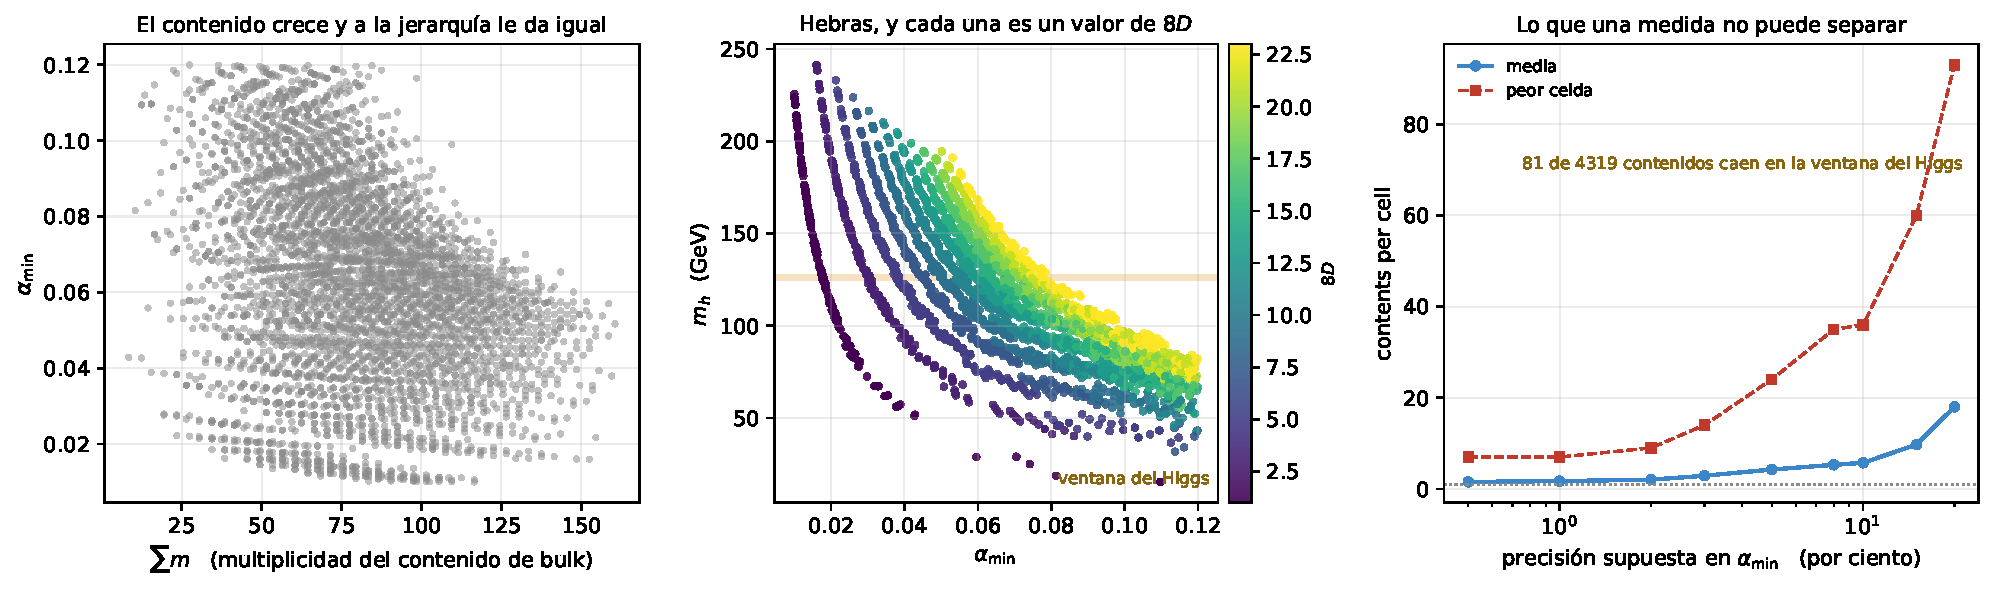
\includegraphics[width=\textwidth]{fig_collapse_lattice_es.pdf}
\caption{\textbf{La aritmética, vista desde el lado de los observables.} Todo contenido construido
con a lo sumo cuatro copias de cada uno de los ocho multipletes, conservado cuando $0<D\le3$ y
$\amin\in[0.010,0.120]$: $4319$ de ellos. \emph{Izquierda:} $\amin$ frente a la multiplicidad total
del contenido de bulk. No hay relación ---a la jerarquía no le importa cuánta materia hay, sino cómo
está repartida entre carga y paridad. \emph{Centro:} los mismos contenidos en el plano de los dos
observables que predicen. La nube se separa en hebras, y cada hebra es un valor de $8D$; la ventana
del Higgs las cruza, de modo que qué contenidos son viables es una pregunta sobre el segundo momento
y no sobre el tamaño del modelo. Coloreado por multiplicidad, ese mismo panel no enseña nada.
\emph{Derecha:} cuántos contenidos comparten una celda del plano de observables, frente a la
precisión supuesta en $\amin$ ---con el lado de $m_h$ de la celda relajado a la vez, de $1$ a
$5$~GeV, porque una medida que afloja lo uno afloja lo otro---. En la celda más fina dibujada la
media es $1.55$ y la peor contiene $7$; en la más holgada, $20\%$ en $\amin$ y $5$~GeV en $m_h$, la
media es $18.0$ y la peor contiene $93$. Los
dos observables determinan el contenido, pues, sólo en la medida en que estén bien medidos, y la
cuantización de la \S\ref{sec:arith} es lo que fija la escala de ese intercambio. $81$ de los $4319$
caen dentro de $125$--$127$~GeV.}\label{fig:collapse}
\end{figure}

\bridge{Dos momentos cuantizados, un núcleo universal, y una jerarquía que es su cociente. ¿Cuál es
la mayor jerarquía que permite el retículo?}

% ===================================================================
\section{El techo}\label{sec:ceiling}

\paragraph{Primero, dos identidades sin logaritmo dentro.} Escríbase
$\mu = m_h^2/(K\pi^2)^2$ ---la masa del Higgs en las unidades en que trabaja el potencial. Eliminar
el logaritmo entre \eqref{eq:fpp} y el punto fijo \eqref{eq:amin} deja
\begin{keyeq}
\begin{equation}\label{eq:two}
  \text{(I)}\quad \ln x \;=\; \frac{G-3\mu}{A_4}-\frac34\,,
  \qquad\qquad
  \text{(II)}\quad x^2 \;=\; \frac{12\,\zeta(3)\,D}{6\mu+A_4}\,.
\end{equation}
\end{keyeq}
\noindent Las dos quedan verificadas a $6\times10^{-14}$ sobre las cinco filas publicadas ---y ese
número hay que leerlo por lo que es. (I) y (II) se obtienen \emph{algebraicamente} de
\eqref{eq:fpp} y \eqref{eq:amin}, así que $6\times10^{-14}$ pone a prueba la implementación y el
álgebra y nada más: una identidad derivada de un desarrollo truncado se verifica a precisión de máquina heredando
íntegro el error de truncamiento de sus padres. La validación física es otra
medida y es la de la \S\ref{sec:closed}: $0.13\%$ de mediana y $0.62\%$ en el peor caso contra la
minimización numérica del potencial sin truncar. Exactitud interna y precisión externa son dos
afirmaciones distintas y aquí se mantienen separadas. La útil es
la (II): \emph{una vez fijada la masa del Higgs, $\amin$ es algebraico en los dos momentos} ---sin
punto fijo y sin logaritmo. Como $1/R_5=2\pi m_W/x$, maximizar la escala de compactificación
significa hacer $D$ pequeño y $A_4$ grande; y $D$ no puede bajar de $1/8$ por el
Teorema~\ref{thm:eighths}. Así que el techo es la pregunta de hasta dónde puede empujarse $A_4$
antes de que la (I) se quede sin contenidos que la satisfagan.

\paragraph{Esa pregunta es un programa entero.} Los tres momentos son \emph{lineales} en el vector
de multiplicidades $n\in\ZZ_{\ge0}^8$, y $A_4$ y $8D$ son enteros. Para un contenido situado en
$(A_4,8D)=(t,k)$ cuya masa del Higgs esté en el techo de la ventana, la (II) fija $x$ sin dejar
libertad alguna, y la (I) exige entonces un valor concreto de $G$:
\begin{equation}\label{eq:gstar}
  G^\star(t,k)\;=\;t\Bigl(\ln x+\tfrac34\Bigr)+3\mu\,,\qquad
  x=\sqrt{\frac{12\zeta(3)(k/8)}{6\mu+t}}\,,
\end{equation}
de modo que el par $(t,k)$ es realizable sólo si algún contenido allí tiene $G\le G^\star(t,k)$.
Relajar las multiplicidades a los reales convierte ``el menor $G$ en $(t,k)$'' en un programa lineal
con dos restricciones de igualdad ---cuyo \emph{dual} tiene por tanto dos variables
\cite{Schrijver}, así que sus
vértices se pueden enumerar exactamente en aritmética racional, redondeando $\ln 2$ y $\ln 3$ en la
dirección que mantiene la cota como cota. Los $(t,k)$ admisibles están restringidos por el
Teorema~\ref{thm:mod6}, y la restricción muerde: el óptimo de la relajación cae en $(216,1)$, donde
$216+1$ no es divisible por tres, así que allí no hay contenido ninguno. La Figura~\ref{fig:cone} es
el retículo sobre el que corre el programa, y su panel derecho es de dónde sale el uno de cada seis.

\begin{figure}[t]\centering
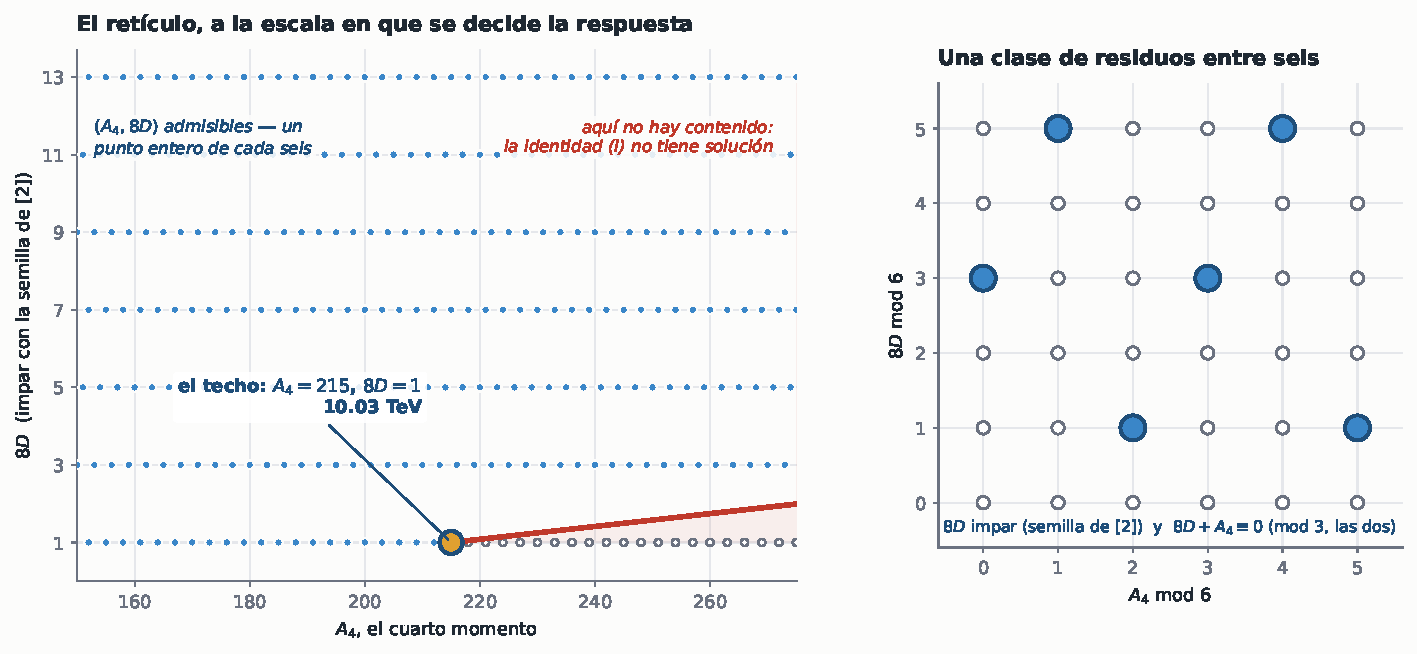
\includegraphics[width=\textwidth]{fig_cone_es.pdf}
\caption{\textbf{El retículo sobre el que corre el programa entero.} A la izquierda, a la escala en que se decide la respuesta: los $(A_4,8D)$ admisibles son un punto entero de cada seis, la curva roja es donde la identidad (I) se queda sin contenidos en la relajación, y los puntos huecos más allá son irrealizables. El máximo de la relajación se sitúa en el último punto admisible de la fila $8D=1$ ---y la Figura~\ref{fig:lift} muestra que \emph{ese} punto está vacío en cuanto se cuenta la tercera coordenada, así que el máximo entero es el de debajo. A la derecha, por qué uno de cada seis: $8D$ impar con la semilla que \cite{KM25} imprimen, que es el Corolario~\ref{cor:kmseed}, junto con $8D+A_4\equiv0\pmod3$, que es el Teorema~\ref{thm:mod6} con las dos semillas. La geometría está calculada exactamente en Sage: el cono tiene rayos extremos $(0,-1)$ y $(1,8)$, descripción dual $\{A_4\ge0,\ 8D\le 8A_4\}$, y los ocho multipletes generan un subretículo de índice exactamente $6$ en $\mathbb{Z}^2$ ---la congruencia, reenunciada como un índice de retículo. Su base de Hilbert es $\{(0,-1),(1,8)\}$, y $(0,-1)$ \emph{no} es alcanzable: el $\mathbf{7}^{(+,+)}$ baja de seis en seis, nunca de uno en uno.}\label{fig:cone}
\end{figure}

\begin{keyeq}
\begin{equation}\label{eq:ceiling}
  \boxed{\;\frac{1}{R_5}\;\le\;10.03\ \text{TeV}\;}
  % La linea castellana es ~10 caracteres mas larga que la inglesa y se salia del marco por la
  % derecha: el borde cortaba la D de D=1/8.  Lo vio Carles leyendo el PDF, no una compuerta --
  % check_layout mide bandas verticales y desbordamiento por abajo, NO por los lados.  Se recorta
  % «de bulk», que el parrafo anterior ya dice, y \qquad pasa a \quad.
  \quad\text{certificado en } A_4=215,\ D=\tfrac18 .
\end{equation}
\end{keyeq}

\noindent \textbf{Y el cuantificador merece decirse exacto.} El dual certifica cada peldaño sobre
el que se corre, para contenido arbitrario \emph{en ese peldaño}. Extenderlo a un máximo sobre
\emph{todos} los peldaños usa una cosa más: que $t^\star(k)/k$ no crezca. Eso estuvo dos semanas
medido hasta $k=501$, y está demostrado dos párrafos más abajo.

\noindent El techo por cada $D$ decrece monótonamente ---$10.03$, $6.27$, $4.21$, $3.14$,
$2.80$~TeV en $8D=1,3,9,33,129$--- y se aplana hacia unos $2.7$~TeV. De modo que el máximo se sitúa
\emph{sobre el cuanto} $D=1/8$: la Parte~VI observó que los ocho contenidos de $\amin$ menor tenían
todos $D=1/8$; aquí eso no es una observación sobre una enumeración, sino dónde está el máximo del
argumento, y el trabajo físico lo hace el Teorema~\ref{thm:eighths}. Esa monotonía conviene decirla
con cuidado, porque todo el techo se apoya en ella. De la (II), $(1/R_5)^2\propto(6\mu+t^\star(k))/k$
con $t^\star(k)$ el mayor $A_4$ admisible en el peldaño $k$, así que una condición \emph{suficiente}
es que $t^\star(k)/k$ no crezca ---y no crece: cae de $215$ en $k=1$ a $70$ en $k=9$ y a $50.8$ en
$k=501$, monótonamente en cada paso---. Medido en \texttt{fissures.py}.

\paragraph{Y es un signo, no un barrido.} Como $1/R_5=2\pi m_W/x$ y la (II) fija $x$, el techo
depende del peldaño \emph{sólo} a través de la pendiente $r_k=t^\star(k)/k$:
\begin{equation}\label{eq:slope}
  M(k)^2\;=\;\frac{8\pi^2m_W^2}{3\zeta(3)}\Bigl(r_k+\frac{6\mu}{k}\Bigr),
\end{equation}
así que la pregunta es una derivada de una función de una variable. La zanjan dos hechos. Primero,
el dual del programa de la \S\ref{sec:ceiling} tiene \textbf{exactamente dos vértices}, y \emph{uno}
de ellos está activo en todos los peldaños ---de modo que el argumento afín a trozos tiene un solo
trozo y no hay fronteras que comprobar. Segundo, poniendo $t=rk$ resulta
$x^2=(3\zeta(3)/2)/(r+6\mu/k)$, y la condición del vértice activo pasa a ser $\Phi(r,k)\ge0$ con
$\Phi=r\bigl(A-\tfrac12\ln(r+6\mu/k)\bigr)-\nu-C/k$,
$A=\tfrac12\ln\tfrac{3\zeta(3)}2+\tfrac34-\lambda$ y
$C=G_{\text{gauge}}-\lambda A_{\text{gauge}}-\nu\,(8D)_{\text{gauge}}-3\mu$. Entonces
\begin{equation}\label{eq:dphidk}
  k^2\,\frac{\partial\Phi}{\partial k}\;=\;\frac{3\mu\,r}{r+6\mu/k}\;+\;C ,
\end{equation}
cuyo primer término es positivo y estrictamente menor que $3\mu$. Así que
$\partial\Phi/\partial k<0$ en cuanto $C\le-3\mu$, que es el enunciado
$G_{\text{gauge}}-\lambda A_{\text{gauge}}-\nu(8D)_{\text{gauge}}\le0$ ---\textbf{una condición
sobre el sector gauge y nada más}, y se cumple con holgura: $-37.43\le0$. Con
$\partial\Phi/\partial r<0$ en la raíz superior, $dr^\star/dk<0$. Los dos términos de la
\eqref{eq:slope} caen, luego $M(k)$ decrece estrictamente, y como el techo en enteros nunca supera al
de la relajación real, $M(k)\le M_{\text{real}}(3)=6268$~GeV para todo $k\ge3$, por debajo de los
$10\,034$~GeV de $8D=1$. \textbf{El máximo se sienta en el cuanto porque no le queda otra.}

\paragraph{Y el aplanamiento tiene un valor.} El límite de $\Phi$ a $k$ grande se deshace de $k$
por completo y deja $r(A-\tfrac12\ln r)=\nu$, una ecuación de Lambert cuyas dos ramas reales son los
extremos de un intervalo de pendientes admisibles: $r=-2\nu/W(-2\nu e^{-2A})$. Intersecando los
intervalos de los dos vértices,
\begin{equation}\label{eq:rinf}
  r_\infty=50.6809086439,\qquad
  M_\infty=\sqrt{\tfrac{8\pi^2m_W^2}{3\zeta(3)}\,r_\infty}=2\,678~\text{GeV},
\end{equation}
aproximado por arriba y nunca alcanzado. De modo que los $2.7$~TeV hacia los que se aplana la tabla no
son una coincidencia numérica: son el rayo asintótico del cono factible, y el techo va de
$10.03$~TeV en el peldaño más pequeño ---con la semilla que \cite{KM25} imprimen, porque cuál es el
peldaño más pequeño lo decide la semilla--- a $2.678$~TeV en el infinito. La asíntota, en cambio, no
es condicional: no lleva ninguna cantidad gauge dentro. Medido en
\texttt{asymptotic\_\allowbreak ray.py}.

\paragraph{Un número nuestro, corregido.} Una nota anterior de esta serie citaba $1/R_5\le2.18$~TeV
bajo la misma ventana del Higgs. Eso es una cota sobre el \emph{tamaño} del contenido ---es lo que
devuelve una enumeración sobre contenidos de a lo sumo seis multipletes, siendo seis el tamaño usado
en su Tabla~1--- y no una cota sobre el modelo, que no acota el contenido en absoluto. Levantando el
tope:

\begin{center}\small
\rowcolors{2}{white}{softgrey}
\begin{tabular}{crrcl}
\toprule
\rowcolor{hdrblue!10}$N$ & en ventana & mejor $1/R_5$ & $D$ & contenido\\
\midrule
$5$  & $1$    & $1924$ & $29/8$ & $\rep{28}^{++}+4\times\rep{84}^{++}$\\
$6$  & $3$    & $2182$ & $21/8$ & $\rep{28}^{++}+\rep{28}^{+-}+\rep{48}^{++}+3\times\rep{84}^{++}$\\
$7$  & $15$   & $3604$ & $7/8$  & $3\times\rep7^{++}+2\times\rep{28}^{++}+2\times\rep{84}^{++}$\\
\rowcolor{amber!14}$8$  & $30$   & $\mathbf{9138}$ & $\mathbf{1/8}$ & $3\times\rep7^{++}+\rep7^{+-}+2\times\rep{48}^{++}+\rep{48}^{+-}+\rep{84}^{++}$\\
$14$ & $1097$ & $9156$ & $1/8$  & $4\times\rep7^{++}+2\times\rep{28}^{++}+5\times\rep{28}^{+-}+\rep{84}^{++}$\\
\bottomrule
\end{tabular}
\end{center}

\noindent El salto está entre siete y ocho multipletes y es un factor $2.5$: ocho es donde el
retículo consigue por primera vez situarse en $D=1/8$ \emph{dentro} de la ventana del Higgs. Dos
multipletes más que los que usa su Tabla~1, no setenta. La Figura~\ref{fig:ceiling} dibuja las dos
mitades de la afirmación: el salto frente al tope al contenido, y la monotonía del techo en $D$.

\begin{figure}[t]\centering
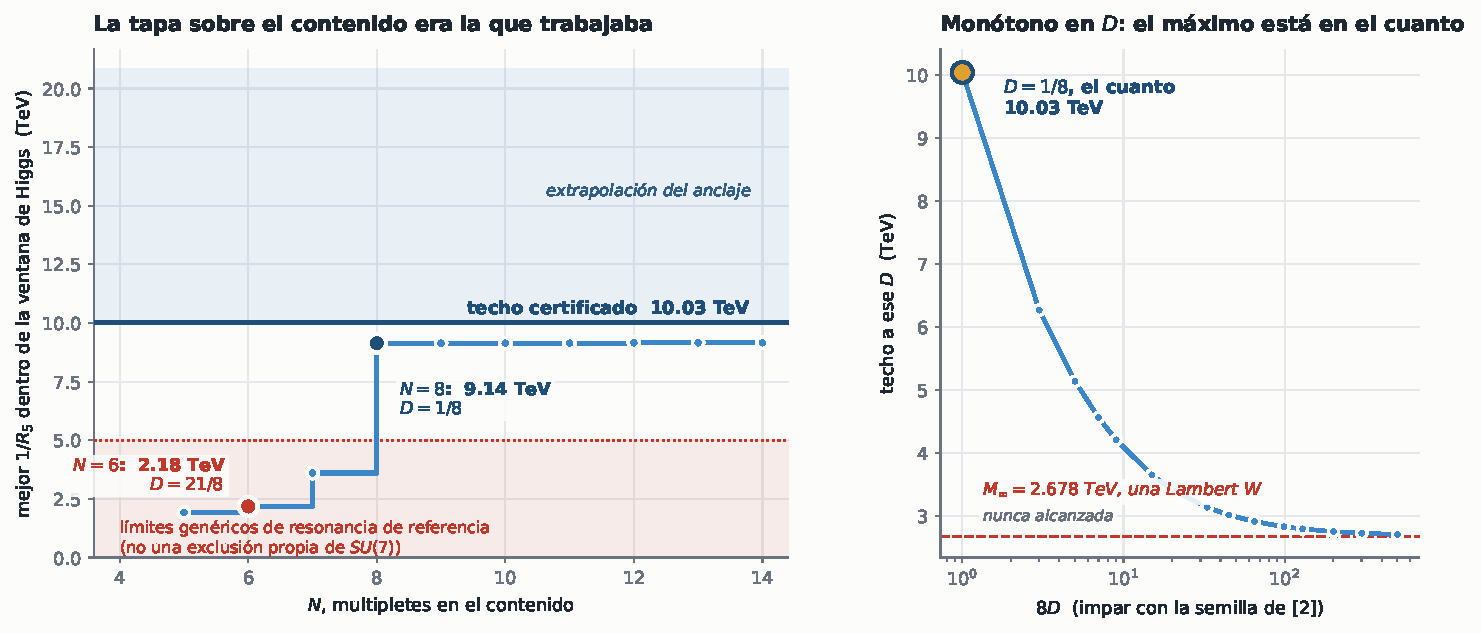
\includegraphics[width=\textwidth]{fig_ceiling_es.pdf}
\caption{\textbf{El tope al contenido era lo que hacía el trabajo.} A la izquierda: el mejor $1/R_5$ dentro de la ventana del Higgs frente al número de multipletes permitidos. Los $2.18$~TeV citados antes en esta serie son el punto $N=6$; en $N=8$ el retículo alcanza por primera vez el cuanto $D=1/8$ de la semilla que \cite{KM25} imprimen y la escala salta un factor $2.5$. La línea horizontal es el techo certificado, la banda por encima la \emph{extrapolación} del anclaje de la \S\ref{sec:setting} ---que la propia \S\ref{sec:setting} tiene cuidado de llamar tendencia y no incertidumbre, y así la rotula también la figura---, y la región sombreada el alcance de las búsquedas genéricas de resonancias de referencia ---\textbf{no una exclusión propia de $\su7$}: la \S\ref{sec:collider} muestra que esos límites se fijan sobre una resonancia \emph{estrecha} y no se trasladan a un objeto con $\Gamma/M\simeq0.16$ y un $\mathrm{BR}(G_1\to jj)$ sin fijar. A la derecha: el techo como función de $D$ ---monótono, de modo que el máximo se sitúa sobre el cuanto, que es el Teorema~\ref{thm:eighths} haciendo trabajo físico.}\label{fig:ceiling}
\end{figure}

\paragraph{Y esa tabla es donde el certificado deja de ser la respuesta.} El óptimo de la relajación
se sienta en $(A_4,8D)=(215,1)$ y la enumeración sólo sube a $9.16$~TeV. El dual acota el cono completo, y eso es un teorema; si un contenido entero \emph{se sienta} en el vértice que certifica es
otra pregunta, y es decidible en vez de abierta ---porque en las coordenadas adecuadas la
obstrucción deja de ser trascendente.

Escríbase $G$ exactamente. Las cargas son $c\in\{1,2,3\}$, así que $A_4^{L}$ y $B_4$ sólo aportan
$\ln 2$ y $\ln 3$, y
\begin{equation}\label{eq:UV}
  G\;=\;\tfrac{25}{12}A_4\;-\;U\ln 2\;-\;V\ln 3\,,
\end{equation}
con $U$ semientero y $V$ entero, los dos lineales en las multiplicidades. Como $\ln2/\ln3$ es
irracional ---$2^q=3^p$ no tiene solución---, el par $(U,V)$ no se pierde dentro de $G$, y el
contenido vive sobre un retículo \emph{tetradimensional} $(A_4,8D,2U,V)$ y no sobre el bidimensional
de la Figura~\ref{fig:cone}. Con la cuarta coordenada conviene ir despacio, porque hay un paso en
falso tentador: $\ln3$ entra por el único generador $\rep{84}^{(+,-)}$, luego
$V=81\,n_{\rep{84}^{(+,-)}}$ ---y eso hace a $V$ barato de describir, pero \emph{no} lo hace
dependiente de los otros tres. Los siete generadores con $V=0$ ya alcanzan rango tres en
$(A_4,8D,2U)$, de modo que el octavo sólo puede añadir dirección, y el rango es cuatro.

El objeto correcto es entonces el grupo finito $\ZZ^r/L$, cuyos factores invariantes son las
congruencias. Una forma normal de Smith da
\begin{equation}\label{eq:snf}
  \ZZ^2/L\cong\ZZ_6\,,\qquad
  \ZZ^3/L\cong\ZZ_2\times\ZZ_{72}\,,\qquad
  \ZZ^4/L\cong\ZZ_{18}\times\ZZ_{648}\,,
\end{equation}
de órdenes $6$, $144$ y $11664$. Así que la ley proyectada del Teorema~\ref{thm:mod6} es la única
congruencia $\ZZ_6$, y el contenido levantado son \textbf{dos} congruencias y no una: un índice es
el orden de un grupo, no un recuento de condiciones, y el número de condiciones independientes es a
lo sumo el rango. Dos secciones anteriores llevaban describiendo este retículo sin nombrarlo.
La \S\ref{sec:closed} es la que autoriza la base: el contenido trascendente de todo el potencial es
$\{\zeta(5),\zeta(3),\ln x,\ln 2,\ln 3\}$ y nada más, así que $\{1,\ln2,\ln3\}$ no es un
truncamiento cómodo sino el generado completo. Y el cambio de paridad sin logaritmo en carga dos de
la \S\ref{sec:ladder}, \eqref{eq:c2flip}, es exactamente la dirección con $\Delta U=\Delta V=0$: el
único movimiento de generador que el tercer eje no ve, y por eso su $\Delta G$ salía racional. La
Figura~\ref{fig:lift} son las dos imágenes una al lado de la otra.

\paragraph{Y levantarlo una vez más lo cierra, porque la quinta coordenada es $2W$.} Subir $W$ como
coordenada en vez de como cribado ---la Figura~\ref{fig:lift} con un eje más--- da
$(A_4,8D,2U,V,2W)$, entero en todas sus entradas una vez
doblados $U$ y $W$, de rango \emph{cinco}, con
\begin{equation}\label{eq:snf5}
  \ZZ^5/L\;\cong\;\ZZ_2\times\ZZ_{72}\times\ZZ_{2592},\qquad\text{índice }373\,248 .
\end{equation}
Cinco es también la dimensión del espacio de funciones de la \S\ref{sec:closed}, y eso no es
casualidad:
\begin{theorem}[invariantes completos]\label{thm:complete}
Dos contenidos de bulk tienen el mismo potencial a un lazo, como función de $\alpha$, si y sólo si
coinciden en $(A_4,8D,2U,V,2W)$.
\end{theorem}
\noindent La demostración son dos núcleos que se encuentran. El mapa contenido $\mapsto$ potencial
tiene núcleo de dimensión tres, generado por la \eqref{eq:fivegen}; el mapa contenido $\mapsto$ las
cinco coordenadas lo tiene de dimensión tres porque el rango es cinco; y el primero está contenido
en el segundo porque cada coordenada es un funcional lineal del potencial. Dimensiones iguales y uno
dentro del otro los hacen iguales. Aquí los dos núcleos se calculan por rutas que no comparten
aritmética ---uno desde los vectores de Fourier, otro desde las definiciones de los momentos--- y
salen generador a generador el mismo. La Figura~\ref{fig:kernel} es el enunciado y su razón, uno al
lado del otro.

\paragraph{Lo que de eso no es nuevo, y un caso está impreso.} Que el potencial sea una \emph{forma
lineal en el contenido del bulk}, con el sector gauge como término constante, es estándar y está
explícito: la ec.~(3.20) de \cite{HY04} escribe exactamente eso y cierra diciendo que \emph{«esta
regla de recuento para los coeficientes del potencial efectivo es aplicable en general»}, y las
ecs.~(2.7) y (2.9) de \cite{CCD24} lo reenuncian. Luego \emph{existen} contenidos degenerados por
puro recuento, y hay uno impreso: la ec.~(3.26) de \cite{CCD24} tiene dos modelos SU(6) cuyos
fermiones de bulk difieren ---dos $\rep{15}$ contra $\rep6+\rep{\bar6}+\rep{20}$--- y cuyos
potenciales para el escalar gauge coinciden idénticamente, anotado como \emph{«accidentalmente el
mismo»}. \textbf{Eso es un elemento del núcleo de abajo, y no es un accidente.} Hay un segundo sin
comentar en las ecuaciones del antecesor pentadimensional de este modelo: las ecs.~(3.10)--(3.12)
de \cite{KTY17} descomponen $\rep{21}$, $\rep{28}$ y $\rep{48}$, y $\rep{21}\oplus\rep{28}$
reproduce la descomposición del $\rep{48}$ término a término, siendo el sobrante $49-48=1$ un
singlete que el potencial no puede ver.

\noindent Tampoco es nueva la idea de reducir la dependencia en el contenido a una lista corta. Las
ecs.~(4.13)--(4.14) de \cite{HHK03} reducen una energía de vacío supersimétrica de Scherk--Schwarz
a \emph{dos} funcionales enteros $a$ y $b$, y su $b=n_F^{(+)}-n_F^{(-)}$ es $W$ en otra notación:
su $h(N)-h(0)=-Nb$ es nuestro $F(1)-F(0)$, un recuento con signo de la materia por paridad que
decide cuál de dos puntos simétricos gana.\footnote{Su ec.~(4.7) sustituye
$N_{\rm Ad}^{(+-)}+N_{\rm Ad}^{(-+)}=(p+s)(q+r)$ donde su propia ec.~(3.20) da el doble; el factor
es inerte, porque su ec.~(4.13) usa el valor correcto, pero la (4.7) es donde queda fijado el
término del sector gauge y ese coeficiente es justo el que este párrafo usa. Rehecho desde sus
ecs.~(4.5)--(4.6) en \texttt{hhk\_\allowbreak gauge\_\allowbreak offset.py}.} Lo que \emph{ellos}
calculan, y lo dicen cuatro veces, su resumen incluido, es la energía de vacío \emph{a fase de
Wilson nula}: su $h(x)$ es función de un entero de condición de contorno, no de la fase.

\noindent Así que lo que se añade aquí son tres cosas, y ninguna es el fenómeno. La base es
\emph{irredundante} ---la lista ingenua de coeficientes cuenta de más, y es la propia ec.~(2.11) de
\cite{CCD24} la que dice cuánto, uso que ellos le dan sólo como simplificador algebraico. El núcleo
es un \emph{subespacio con generadores}, la \eqref{eq:fivegen}, y no una lista de accidentes;
ningún enunciado de la forma «estos invariantes son completos» aparece en \cite{HY04,HHK03,CCD24},
ni ninguno de ellos cuenta la dimensión del espacio de potenciales alcanzables. Y los invariantes
son de una clase particular: $A_4$, $U$ y $V$ salen del \emph{desarrollo a $\alpha$ pequeño}, de
modo que el Teorema~\ref{thm:complete} dice que datos locales del desarrollo junto con una única
comparación global, $W$, fijan el potencial en todo $[0,1]$. Eso último sólo vale la pena decirlo
porque el espacio es de dimensión cinco y no uno: si fuera uno, el teorema sería la linealidad
reenunciada. \textbf{El retículo de esta sección y el espacio de funciones de la \S\ref{sec:closed}
son un solo objeto}, y esos cinco números son coordenadas sobre él.

\paragraph{Lo que hace que las tres paridades sean heredadas ---y, resulta, no heredadas juntas.}
Todo multiplete de materia aporta una cantidad \emph{par} a $8D$, a $2U$ y a $2W$. Eso es robusto y
es propiedad del contenido y de nada más: las tres paridades las decide el sector gauge, y ningún
contenido del bulk puede tocarlas. Con los coeficientes que \cite{KM25} imprimen, el sector gauge
aporta $-27$, $-39$ y $-3$ ---impares los tres---, de modo que para todo contenido de bulk
\begin{equation}\label{eq:parity3}
  8D\;\equiv\;2U\;\equiv\;2W\;\equiv\;1\pmod 2 .
\end{equation}

\noindent \textbf{Pero eso es un enunciado sobre esta semilla, no una identidad estructural, y no
pudimos ver la diferencia hasta que hubo una segunda semilla contra la que contrastarlo.} Una
versión anterior de este párrafo leía la \eqref{eq:parity3} como una sola congruencia sobre tres
coordenadas, con origen en el único semientero $-\tfrac72$. Sustitúyase el reparto candidato
gauge-más-fantasma de la \S\ref{sec:open} y las tres se separan: $8D$ pasa de $-27$ a $-18$ y $2U$
de $-39$ a $-30$, perdiendo las dos su imparidad, mientras $2W$ se queda en $-3$. \emph{La paridad
de $2W$ es robusta. La de $8D$ no.}

\noindent La razón se lee en las coordenadas, y es más bonita que la afirmación a la que sustituye.
El candidato mueve los dos pesos de carga uno, el periódico y el antiperiódico, en el mismo
$+\tfrac12$, y el de carga dos en $+\tfrac14$. Al recogerlos, $8D$ y $2U$ se desplazan exactamente
$9$ cada uno ---impar, luego los dos voltean--- mientras que $2W$ depende de la \emph{diferencia}
$-u_{(+,1)}+u_{(-,1)}$, en la que los dos desplazamientos de medio se cancelan, y se mueve $0$. Así
que sí hay un mecanismo compartido, pero no el que afirmábamos: es que el sector gauge suministra
las tres paridades, y $2W$ es la única combinación a la que un desplazamiento uniforme de los pesos
de carga uno no llega. \textbf{Un teorema que sobrevive a un cambio de hipótesis vale más que uno
que no, y hasta tener la segunda semilla no teníamos manera de saber cuál de los nuestros era
cuál.} La
tercera lectura, $2U$ impar, se enuncia porque lo dice el carácter; qué le prohíbe hacer a un
contenido no se sabe aquí, y $A_4$ y $V$ no quedan forzadas, así que la \eqref{eq:parity3} es un
enunciado sobre \emph{cuáles} tres. No es, en cambio, una lectura independiente: la
\eqref{eq:congr5} hace \emph{equivalentes} en cualquier contenido que $2U$ sea impar y que $2W$ lo
sea, por una congruencia que no menciona el $-\tfrac72$ en ningún momento.
Calculado en \texttt{lattice\_\allowbreak lift.py} e
independientemente, con las matrices de transformación y las tres congruencias escritas, en
\texttt{lattice\_\allowbreak lift.sage}.

\begin{figure}[t]\centering
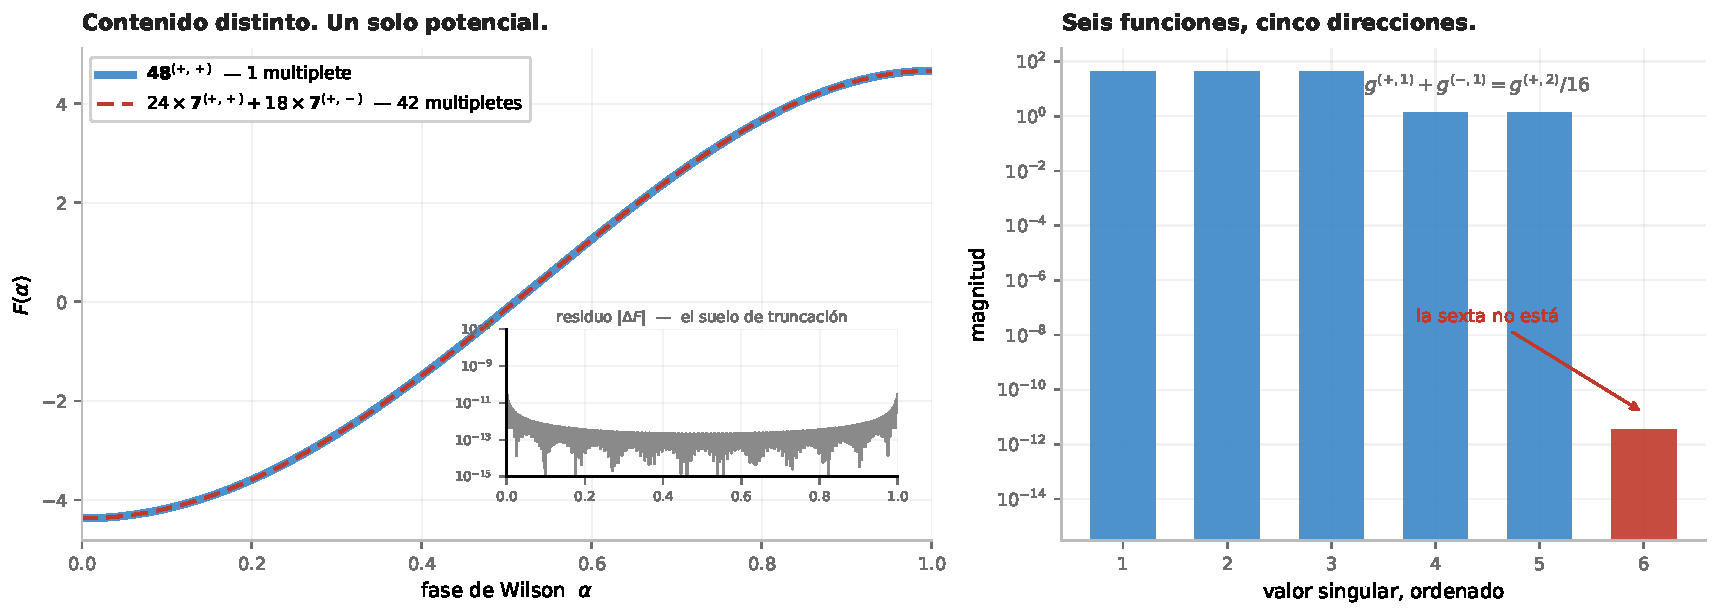
\includegraphics[width=\textwidth]{fig_kernel_es.pdf}
\caption{\textbf{El Teorema~\ref{thm:complete}, en las dos mitades de las que está hecho.}
\emph{Izquierda:} lo que afirma. Un solo $\rep{48}^{(+,+)}$ y
$24\times\rep7^{(+,+)}+18\times\rep7^{(+,-)}$ ---un multiplete contra cuarenta y dos,
representaciones distintas, dimensiones distintas--- dan \emph{una sola curva}, sobre el potencial
polilogarítmico exacto y en todo el dominio fundamental. El recuadro es el residuo: sobre $1600$ puntos de
$[0,1]$ su peor valor es $2.9\times10^{-11}$, que no es la identidad fallando sino el suelo de \emph{esta} evaluación, la truncación
de la suma de enrollamientos a $600$ modos. La relación es exacta sobre $\mathbb{Q}$, demostrada en
\texttt{dimension\_\allowbreak five.sage}. \emph{Derecha:} por qué ocurre. Las seis funciones
$\mathrm{Re}\,\mathrm{Li}_5(s\,e^{ic\pi\alpha})$ parecen seis direcciones y son cinco: tres valores
singulares de orden $45$, dos de orden $1.4$, y un sexto en $3.5\times10^{-12}$ ---once
órdenes por debajo del menor de los cinco. La que falta es la fórmula de duplicación en
$s=5$, que es la ec.~(2.11) de \cite{CCD24}. Un contenido es invisible al potencial exactamente
cuando es invisible a esas cinco, que es el teorema. Dibujada por
\texttt{make\_\allowbreak fig\_\allowbreak kernel.py}.}\label{fig:kernel}
\end{figure}

Eso es lo que hace decidible el vértice. A $(A_4,8D)$ fijos, la condición $G\le G^\star$ se lee
$U\ln2+V\ln3\ \ge\ \tfrac{25}{12}A_4-G^\star$: maximizar una forma lineal sobre los contenidos con
dos momentos clavados. Todo generador tiene $A_4\ge0$ y sólo el $\rep7^{(+,+)}$ tiene $A_4=0$, cuya
multiplicidad queda entonces forzada por $8D$ ---así que el conjunto factible es \emph{finito} y el
máximo es un cálculo, no una búsqueda. Sale
\begin{center}\small
\begin{tabular}{crrr l}
\toprule
\rowcolor{hdrblue!10}$A_4$ en $8D=1$ & exigido & mayor disponible & déficit & \\
\midrule
\rowcolor{warmred!14}$215$ & $681.084$ & $681.017$ & $-0.067$ & ningún contenido, de ningún tamaño\\
$212$ & $667.670$ & $669.927$ & $+2.257$ & alcanzado\\
\bottomrule
\end{tabular}
\end{center}
\noindent de modo que el vértice de la relajación está \emph{vacío} y el de debajo no ---que es lo
que dibuja la Figura~\ref{fig:lift}, peldaño a peldaño. El techo tiene entonces testigo, y la cota
se afila:
\begin{keyeq}
\begin{equation}\label{eq:ceilinginteger}
  \boxed{\;\frac{1}{R_5}\;\le\;10.01\ \text{TeV}\;}
  \quad\text{óptimo en } A_4=212,\ D=\tfrac18 .
\end{equation}
\end{keyeq}
\begin{figure}[t]\centering
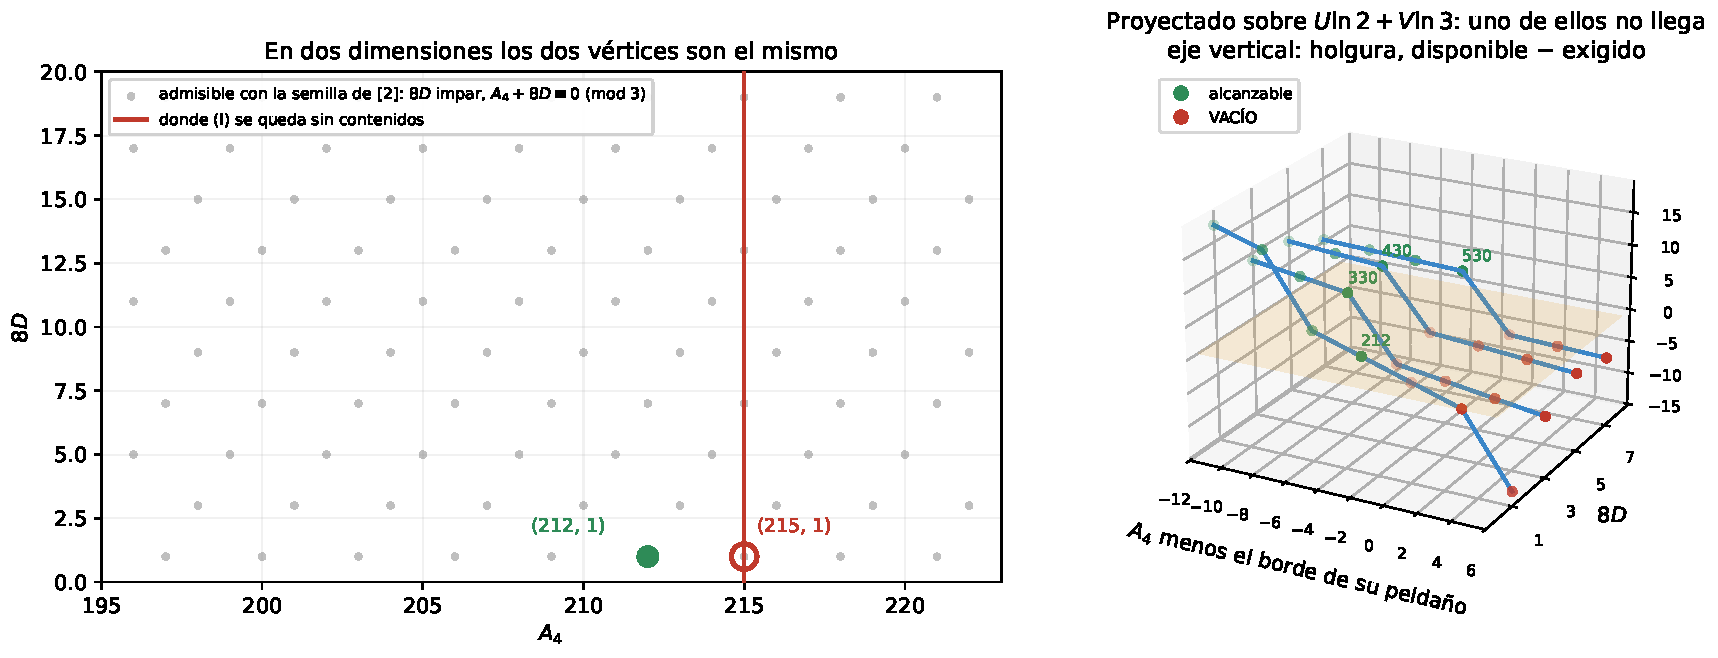
\includegraphics[width=\textwidth]{fig_lift_es.pdf}
\caption{\textbf{El eje que la proyección escondía.} \emph{Izquierda:} el plano en el que se ha calculado el techo. Tanto $(215,1)$ como $(212,1)$ son puntos admisibles del retículo ---$8D$ impar con la semilla que \cite{KM25} imprimen, y $A_4+8D\equiv0\pmod 3$--- y los dos se sientan en el borde o por debajo, donde la identidad~(I) se queda sin contenidos. Nada en esta imagen los separa. \emph{Derecha:} los mismos puntos con la tercera coordenada de \eqref{eq:UV}, dibujada como la \emph{holgura} entre el presupuesto logarítmico que un contenido puede aportar y el que exige $G\le G^\star$; el presupuesto en bruto pasa de $680$ y todo el veredicto mide $0.067$, así que lo que se puede dibujar es la holgura. Cada peldaño va contra la distancia a \emph{su propio} borde, que es lo que hace comparables a los cuatro. El plano ámbar es el cero. Verde alcanzable, rojo vacío, y la etiqueta verde es el óptimo entero de ese peldaño. La holgura cae monótonamente, luego cada cruce es único y cada óptimo está bien definido ---y el patrón es el mismo en todos: \textbf{el borde de la relajación está vacío y el óptimo entero cae uno o dos pasos de tres por debajo}, en $212$, $330$, $430$, $530$ para $8D=1,3,5,7$. Dibujada por \texttt{make\_\allowbreak fig\_\allowbreak lift.py}; la aritmética es \texttt{semigroup.py}.}\label{fig:lift}
\end{figure}

\noindent El testigo es
$17\times\rep7^{(+,+)}+2\times\rep7^{(+,-)}+57\times\rep{28}^{(+,-)}$, setenta y seis multipletes
---grande, y nada en el modelo topa el contenido, que era justo el asunto de la
\S\ref{sec:ceiling}. Tres cosas mantienen eso honesto. El veredicto sobre el $215$ está comprobado a cincuenta
dígitos y en los dos extremos de la ventana del Higgs ---el menor $G$ disponible allí es $-233.100$
frente a un $G^\star(127)=-233.168$, o sea que falla en el extremo \emph{más permisivo} y por tanto
en todos. El testigo se reconstruye por la vía ordinaria de \texttt{moments()}, que no sabe nada de
$U$ ni de $V$, y reproduce $A_4=212$, $8D=1$, $G=-228.260$ dentro de la banda. Y el margen que
separa el $215$ del $212$ es de una parte en $10^{4}$, un orden por debajo del $0.13$--$0.62\%$
propio de la forma cerrada. Medido en \texttt{semigroup.py}.

\paragraph{Y el orden sobrevive al truncamiento, cosa que no era evidente y que estuvo cerca de
fallar.} Todo lo anterior vive sobre la superficie \eqref{eq:amin}, que conserva tres peldaños; el
resto $R$ que se descarta va acotado al final de esta sección, en la \eqref{eq:remainder}, y aquí
sólo hace falta que se pueda \emph{evaluar} sobre el puñado de contenidos en cuestión. Rehacer la
eliminación sin tirarlo da el par corregido
\begin{equation}\label{eq:corrected}
  x^2(6\mu+A_4)=12\zeta(3)D-\frac{18R'(x)}{x}+6R''(x)\,,\qquad
  \ln x=\frac{G-3\mu}{A_4}-\frac34+\frac{3\,[\,xR''(x)-R'(x)\,]}{A_4x^3}\,,
\end{equation}
de modo que el $G^\star$ exigido se desplaza en $\Delta G^\star=-3[xR''-R']/x^3$. Evaluado sobre los
contenidos que de verdad se sientan en esos vértices, $\Delta G^\star\simeq-0.45$ en $(215,1)$ y
$-0.33$ en $(212,1)$ ---\textbf{siete veces los $0.067$ que los separan}. Comparar la corrección con
ese hueco es, por tanto, la prueba equivocada, y vale la pena decir por qué: $\Delta G^\star$ es
\emph{de modo común}, porque los contenidos de los dos vértices se diferencian en unos pocos
multipletes de ochenta. Lo que sí puede hacer es comerse la holgura propia de cada uno, y ésa es la
prueba:
\begin{center}\small
\begin{tabular}{crrrl}
\toprule
\rowcolor{hdrblue!10}vértice & holgura, truncada & $\Delta G^\star$ & holgura, corregida & \\
\midrule
\rowcolor{warmred!14}$(215,1)$ & $-0.067$ & $-0.452$ & $-0.519$ & sigue fallando\\
$(212,1)$ & $+2.257$ & $-0.332$ & $+1.925$ & sigue en pie\\
\bottomrule
\end{tabular}
\end{center}
\noindent \textbf{Los dos veredictos sobreviven: $(215,1)$ falla por más al cargar el truncamiento,
no por menos, y $(212,1)$ conserva $1.93$ de holgura.} Lo que no se reclama es uniformidad:
$\Delta G^\star$ está aquí evaluado sobre los contenidos concretos, con nombre y en número finito,
y no acotado sobre todos ellos, que no es lo mismo.

Y hay además una vía que no necesita corrección ninguna. En $(215,1)$, el menor $G$ disponible entre
los $26933$ contenidos es $-233.100$, mientras que la ventana del Higgs va de $[-238.553,-233.168]$;
como $m_h$ es monótona en $G$ a momentos fijos ---$dG/d\mu=18\mu/(6\mu+A_4)>0$---, todo contenido de
ahí queda por encima de la ventana. Eso es una evaluación sobre un conjunto finito. Medido en
\texttt{certify\_\allowbreak 212\_\allowbreak 215.py}.

\paragraph{Y al llevar el testigo al potencial exacto, suspende una prueba que el certificado nunca
le hizo.} Un testigo es un contenido concreto, de modo que admite evaluación sin desarrollo alguno:
se minimiza el polilogaritmo numéricamente y se mira. El mínimo electrodébil está donde tiene que
estar ---$\alpha=0.016129$ frente al $0.016133$ que predice la forma cerrada, un acuerdo del
$0.02\%$, mejor que en ninguna fila publicada--- y su $m_h=126.25$~GeV cae dentro de la ventana.
Pero en el \emph{otro} punto simétrico, $\alpha=1$, el potencial vale $-204.99$ contra los $+111.44$
de ese mínimo. \textbf{El contenido que alcanza el techo está en un falso vacío.} Las cinco filas
publicadas no lo están, y ése es el control. La Figura~\ref{fig:vacuum} son las dos curvas.

\begin{figure}[t]\centering
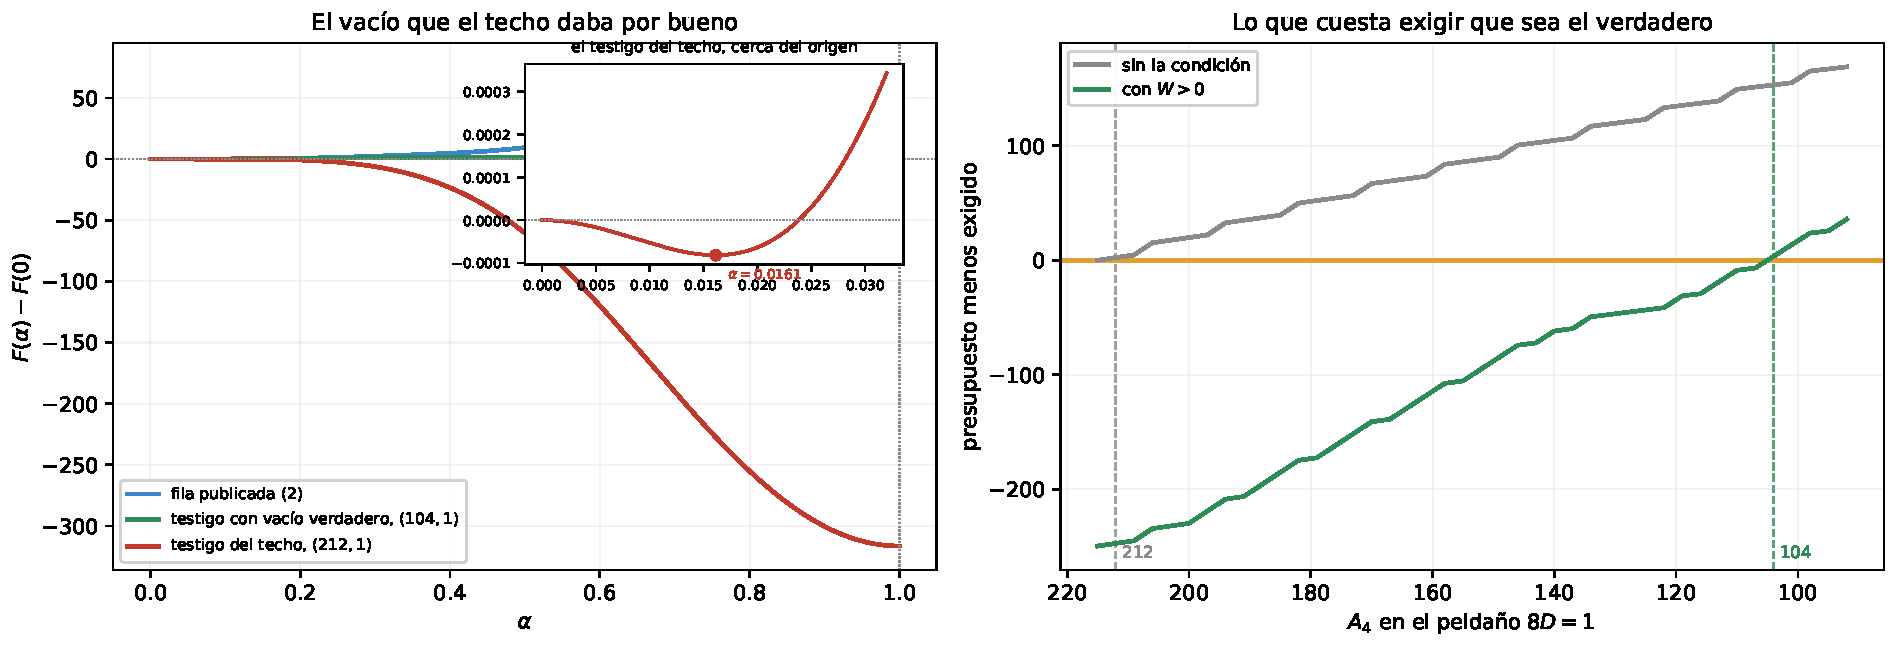
\includegraphics[width=\textwidth]{fig_vacuum_es.pdf}
\caption{\textbf{El vacío que el certificado daba por bueno.} \emph{Izquierda:} el $F(\alpha)$ polilogarítmico exacto sobre el dominio fundamental entero, con cada curva desplazada para que $F(0)=0$. Una fila publicada sube hacia la derecha: su mínimo electrodébil es el punto más hondo que hay. El contenido que alcanza los $10.01$~TeV, en cambio, se despeña ---en el otro punto simétrico, $\alpha=1$, queda $316$ por debajo del origen---, de modo que el mínimo sobre el que se construyó el techo es falso. La tercera curva es el contenido que alcanza el techo restringido de la \eqref{eq:ceilingtrue}: también sube, pero sólo $3.5$, y por eso se pega al eje a esta escala ---pasar la prueba no es lo mismo que pasarla con holgura. El recuadro es ese mismo contenido cerca del origen, donde su mínimo es perfectamente real y cae a un $0.02\%$ de donde lo pone la \eqref{eq:amin}: nada falla en la forma cerrada, sólo en la pregunta que se le hizo. \emph{Derecha:} lo que cuesta excluir contenidos así. En cada vértice del peldaño $8D=1$, el mayor presupuesto logarítmico disponible menos el que exige la \eqref{eq:gstar}, con y sin la condición de estabilidad $W>0$ de la \eqref{eq:truevac}, que es de \cite{CCD24} y no nuestra. La curva sin restringir cruza el cero en $A_4=212$ y la restringida no lo alcanza hasta $A_4=104$; entre esos dos cruces hay $0.8$~TeV de techo. Dibujada por \texttt{make\_\allowbreak fig\_\allowbreak vacuum.py}.}\label{fig:vacuum}
\end{figure}

\paragraph{Ni la prueba que suspende es nuestra, ni la aritmética con que se hace.} Cacciapaglia
\emph{et al.}~\cite{CCD24} enuncian el criterio y demuestran las identidades que necesita, en su
\S2.2. Con sus palabras: \emph{«basta evaluar el potencial en $a=0$ y $a=1/2$ y ver qué
configuración da el valor menor»}; sus ecs.~(2.12)--(2.13) dan $F_+(0)=\tfrac32\zeta(5)>0$ y
$F_-(0)=F_+(1/2)=-\tfrac{15}{16}F_+(0)$, $F_-(1/2)=F_+(0)$; y la conclusión la sacan ellos ---las
componentes de paridad $(\pm,\pm)$ estabilizan el orbifold de partida y las $(\pm,\mp)$ lo
desestabilizan. \textbf{El criterio, su aritmética y su regla de signos son suyos, los tres.}
Sumando su (2.13) sobre un contenido de bulk en la contabilidad de la \eqref{eq:F}, donde su
desplazamiento semientero es nuestro $\alpha\to\alpha+1$ y por tanto sólo se mueven las cargas
impares, queda
\begin{equation}\label{eq:truevac}
  F(1)-F(0)\;=\;\tfrac{31}{16}\,\zeta(5)\,W\,,\qquad W=\sum_{c\ \mathrm{impar}} m\,(-s)\,,
\end{equation}
con $\tfrac{31}{16}=1+\tfrac{15}{16}$, y $W>0$ suficiente para que el punto electrodébil sea el más
hondo de los dos. Eso es su enunciado en nuestra notación y nada más; $W$ es su recuento
estabilizador menos el desestabilizador. Lo nuevo aquí es únicamente el \emph{uso}: $W$ es lineal en
las multiplicidades, como $A_4$, $8D$ y $G$, así que cabe dentro del mismo programa entero ---y
\cite{CCD24} no calculan ninguna escala de compactificación, de modo que allí no hay programa donde
meterlo. Para este modelo los valores por multiplete son $\pm1,\pm3,\pm6,\pm9$ para
$\rep7,\rep{28},\rep{48},\rep{84}$ y $-\tfrac32$ para el sector gauge, siendo el signo la paridad;
las cinco filas publicadas tienen
$W=\tfrac{63}{2},\tfrac{75}{2},\tfrac{75}{2},\tfrac{73}{2},\tfrac{69}{2}$ y el vértice $(212,1)$
tiene $W=-\tfrac{315}{2}$. Comprobado
contra el potencial exacto a precisión de máquina en las seis.

\paragraph{Y $W$ no puede anularse ---por una razón más firme que la del
Teorema~\ref{thm:eighths}.} La materia aporta enteros a $W$. El sector gauge no: su parte de carga
impar es $2-\tfrac72=-\tfrac32$. Por tanto $2W$ es un entero impar para todo contenido de bulk y,
con la \eqref{eq:truevac},
\begin{keyeq}
\begin{equation}\label{eq:nevermarginal}
  \frac{32}{31}\,\frac{F(1)-F(0)}{\zeta(5)}\ \text{es un entero impar, luego}\quad
  |F(1)-F(0)|\;\ge\;\tfrac{31}{32}\,\zeta(5)\,.
\end{equation}
\end{keyeq}
\noindent \textbf{En este modelo los dos puntos simétricos nunca son degenerados} ---y el alcance de
esa frase no es adorno, porque en otros modelos de la misma arquitectura sí lo son: véase abajo.

\noindent \textbf{Y ésta vale en las dos ramas, cosa que los octavos impares no.} Tienta
archivarla junto al Teorema~\ref{thm:eighths} como el mismo semientero leído dos veces, y una
versión anterior de este artículo lo hacía. La semilla candidata de la \S\ref{sec:open} los separa.
Mueve los dos pesos de carga uno en el mismo $+\tfrac12$, y $2W$ depende de la \emph{diferencia}
$-u_{(+,1)}+u_{(-,1)}$, en la que ese desplazamiento se cancela exacto: $2W$ se queda en $-3$. La
contribución gauge a $8D$ no se cancela y se mueve $9$, perdiendo su paridad. \emph{De modo que
$2W$ impar es robusto frente a la semilla y $8D$ impar no lo es} ---y con una sola semilla delante
no habríamos sabido cuál era cuál. Verificado sobre los
$3003$ contenidos de a lo sumo seis multipletes: ninguno tiene $W=0$ ni $2W$ par.

Y eso importa más de lo que parece, porque cierra una cuestión que \cite{CCD24} plantean ellos
mismos. En sus
modelos la degeneración \emph{sí} ocurre, dos veces y exacta: su ec.~(3.14) es función de $2a$ sola,
y su ec.~(3.44) es invariante bajo el desplazamiento simultáneo
$(a,b)\to(a+\tfrac12,b+\tfrac12)$, de modo que en ambos casos los dos puntos simétricos son
degenerados y ellos lo leen bien ---entonces los dos son \emph{«dos descripciones equivalentes del
mismo orbifold»}. Si aquí pasara eso, un potencial más hondo en $\alpha=1$ sería un cambio de
etiqueta y no un falso vacío. Pero descripciones equivalentes han de dar potenciales iguales, y la
\eqref{eq:nevermarginal} dice que esos dos valores nunca lo son ---de modo que en este modelo la
configuración más honda es un orbifold genuinamente distinto, y la lectura de arriba se sostiene.

\noindent \textbf{Y toda la diferencia entre las dos situaciones es un número.} La arquitectura es
común: \cite{HHK03} también reducen su energía de vacío a funcionales enteros y también encuentran
que un recuento con signo por paridad decide entre dos configuraciones simétricas. Pero su sector
gauge aporta el \emph{entero par} $+2$ a su $a$ y nada en absoluto a su $b$, así que los dos pueden
anularse ---abren su clasificación con «el caso $a=0$» y listan
$n_F^{(+)}=n_F^{(-)}\Rightarrow$ «completamente degenerado» como un caso corriente (sus
ecs.~(4.14), (4.15)). Aquí el sector gauge aporta a $W$ un \emph{semi}entero ---$2-\tfrac72=-\tfrac32$ con la semilla
que imprime \cite{KM25} y $\tfrac32-3=-\tfrac32$ con la candidata, el mismo número las dos veces
porque $W$ lee la diferencia---, y un semientero no lo cancelan los enteros. \textbf{El caso degenerado que ellos enumeran es, en este modelo, aritméticamente
inalcanzable.} Medido en \texttt{W\_\allowbreak is\_\allowbreak half\_\allowbreak odd.py} y
\texttt{hhk\_\allowbreak gauge\_\allowbreak offset.py}. El criterio sigue siendo suyo; lo que se
añade es que aquí no puede empatar.

\paragraph{El techo, con el vacío obligado a ser el verdadero.} Imponiendo $W>0$ junto a
$G\le G^\star$ y bajando por el peldaño, ningún vértice sobrevive hasta $A_4=104$:
\begin{keyeq}
\begin{equation}\label{eq:ceilingtrue}
  \boxed{\;\frac{1}{R_5}\;\le\;9.22\ \text{TeV}\;}
  \quad\text{alcanzado en } A_4=104,\ D=\tfrac18,\ \text{con vacío verdadero.}
\end{equation}
\end{keyeq}
\noindent El testigo es
$16\times\rep7^{(+,+)}+\rep{28}^{(+,-)}+\rep{48}^{(+,+)}+4\times\rep{48}^{(+,-)}+\rep{84}^{(+,+)}$,
veintitrés multipletes, $W=\tfrac52$; y sobre el potencial polilogarítmico \emph{exacto} su minimizador
global es $\alpha=0.017560$, con $m_h=126.00$~GeV y $1/R_5=9157$~GeV. \textbf{Ese último número es
una afirmación sobre el potencial y no sobre desarrollo alguno.}

\paragraph{Y hay un segundo número, porque $127$ no es una masa que el Higgs tenga.} Todos los
techos de aquí se evalúan en el tope de la ventana $[125,127]$ de \cite{KM25}, que es el extremo
correcto para una cota superior: $\mu\propto m_h^2$, luego por la (II) el techo sube con $m_h$
---medido, no supuesto. Pero la medida es $m_h=125.20\pm0.11$~GeV, y $127$ está $16.4$ desviaciones
típicas por encima. Evaluado en cambio a la masa que el Higgs tiene de verdad, el vértice baja un
peldaño entero del retículo y la respuesta con él:
\begin{keyeq}
\begin{equation}\label{eq:ceilingmeasured}
  \boxed{\;\frac{1}{R_5}\;\le\;9.09\ \text{TeV}\;}
  \quad\text{en } A_4=101,\ \text{con la masa de Higgs medida.}
\end{equation}
\end{keyeq}
frente a $9.22$~TeV en $A_4=104$ sobre la ventana ---un $1.4\%$, y un paso de tres en $A_4$. La
banda de una sigma \emph{no} mueve el vértice, $125.09$ y $125.31$ dan los dos $101$, de modo que la
\eqref{eq:ceilingmeasured} es estable frente a la medida e inestable sólo frente a la anchura de una
ventana que nadie está obligado a usar. La misma sustitución lleva el techo sin restringir de
$10.01$ a $9.87$~TeV. Los dos enunciados son ciertos y no son el mismo: $9.22$~TeV acota todo
contenido cuya masa de Higgs caiga \emph{en cualquier punto} de $[125,127]$, y $9.09$~TeV acota todo
contenido cuya masa de Higgs sea la medida. \textbf{Quien quiera un número sobre el mundo debe tomar
el segundo.} La ventana se conserva para el titular porque es la de \cite{KM25} y porque una cota
dada sobre una ventana declarada es el objeto más seguro. Medido en
\texttt{higgs\_\allowbreak window.py}.

\paragraph{Y explica un hueco que este artículo había dejado sin explicar.} La tabla de arriba topa
en $9156$~GeV mientras el certificado dice $10034$, y a esa diferencia la llamamos el hueco entre
una relajación y su retículo. No lo es. La enumeración usaba el minimizador \emph{global}, así que
llevaba cribando falsos vacíos todo el tiempo sin decirlo; el certificado no cribaba nada. Sus dos
campeones tienen $W>0$ ---$\tfrac{31}{2}$ en $N=8$ y $\tfrac52$ en $N=14$--- y evaluados exactamente dan $9139$ y
$9157$~GeV, que son los dos números que ya estaban en la tabla. \textbf{El óptimo con la condición
impuesta \emph{es} el campeón de la enumeración}, y un hueco que parecía búsqueda insuficiente era
una condición física que nadie había escrito. Medido en \texttt{socratic\_\allowbreak witness.py} y
\texttt{vacuum\_\allowbreak constraint.py}.

\paragraph{Y la última aproximación que queda \emph{dentro} de la \eqref{eq:F} es el truncamiento,
y va acotada y no estimada.}
Todo lo anterior, salvo las dos evaluaciones exactas, se calcula sobre la superficie
\eqref{eq:amin}, que conserva tres peldaños de la escalera. Escríbase $F=F_0+R$, con $R$ la parte
de $k\ge3$. Dos hechos clásicos hacen acotable a $R$, y ninguno es nuestro:
$\zeta(5-2k)=-B_{2k-4}/(2k-4)$ con $|B_{2n}|\le(\pi^2/3)(2n)!/(2\pi)^{2n}$ \cite{Apostol}, y el
propio desarrollo \cite{Lewin}. Acotando el corchete de la \eqref{eq:ladderab} por el cuarto
momento, $A_4+B_4$, y sumando la geométrica queda, para $u=c_{\max}\alpha<1$,
\begin{equation}\label{eq:remainder}
  |R(\alpha)|\;\le\;\frac{\pi^{6}S_4\,c_{\max}^{2}\,\alpha^{6}}{2160\,(1-u^{2})}\,,\qquad
  |R'(\alpha)|\;\le\;\frac{\pi^{6}S_4\,c_{\max}^{2}\,\alpha^{5}}{360\,(1-u^{2})}\,.
\end{equation}
Sometida a un intento de falsación sobre $32$ contenidos y cuatro valores de $\alpha$ en cada uno
---el intento era encontrar una violación, y el resultado es que no hay ninguna---, con holgura
más ajustada $1.4\times$. Dos controles, y los dos pueden fallar: la cota \emph{se niega} a devolver
nada en $u\ge1$, donde el resto verdadero efectivamente explota; y es una cota, no una estimación
---la estimación afilada es $(A_6+3B_6)x^6/8640$, que no es rigurosa, y confundirlas sería el error
más fácil de cometer aquí. Una versión anterior de la \eqref{eq:remainder} llevaba un factor de
más, y fue la falsación la que lo cazó.

\paragraph{Usarla de la manera obvia no sirve de nada, y ahí está lo instructivo.} Sustituir en cada
peldaño su $1/R_5$ por el valor superior riguroso y volver a maximizar \emph{no} da un techo
riguroso de $10$~TeV: da $52.429$~TeV, y el máximo se muda de $8D=1$ a $8D=139$. El margen crece con
$A_4$ mientras el valor truncado baja, así que los peldaños que pierden en la superficie truncada
ganan en la acotada. \textbf{Una cota sobre el resto no es automáticamente una cota sobre el
óptimo}, y la distinción no es formal: tomarla en serio mueve la respuesta un factor cinco.

\paragraph{Lo que lo repara no es una desigualdad mejor, sino no necesitar ninguna.} Las cargas
recorren $c\in\{1,2,3\}$ y hay dos paridades, de modo que el potencial está generado por seis
funciones \emph{por mucha materia que haya} ---cinco, en realidad, y la reducción \emph{no es
nuestra}. La fórmula de duplicación del polilogaritmo
$\mathrm{Li}_s(z)+\mathrm{Li}_s(-z)=2^{1-s}\mathrm{Li}_s(z^2)$ \cite{Wood} en $s=5$ da
$g^{(+,1)}+g^{(-,1)}=g^{(+,2)}/16$, y \cite{CCD24} escribe justo eso en justo este contexto ---su
ec.~(2.11), $F_-(a)=-F_+(a)+\tfrac1{16}F_+(2a)$, repetida en \cite{Cac25} ec.~(3.3). Aquí no hay
una segunda relación de esa clase porque $c=4$ y $c=6$ no son cargas de este modelo, así que las
seis generan cinco. Abajo sólo se usa que el número sea finito; y el enunciado es sobre
\eqref{eq:F}, la parte $n^{-5}$ del potencial de \cite{KM25}, no sobre su peso de enrollamiento
completo, que mezcla potencias y no cierra en cinco. De ahí que
$R(\alpha)=R_{\text{gauge}}(\alpha)+\sum_j n_j R_j(\alpha)$ exactamente ---la misma forma que
$A_4$, $8D$, $G$ y $W$. El margen es entonces él mismo un funcional lineal y entra en el propio dual
que produce el certificado, con la restricción $G\le G^\star$ soltada para que la respuesta siga
siendo cota y el dual siga siendo de dos variables. Ese movimiento es programación lineal corriente
\cite{Schrijver} y no se reclama como otra cosa. Sobre $70$ peldaños:
\begin{keyeq}
\begin{equation}\label{eq:rigorousceiling}
  \boxed{\;\frac{1}{R_5}\;\le\;10.037\ \text{TeV}\;}
  \quad\text{sin truncar, sobre los primeros $70$ peldaños impares.}
\end{equation}
\end{keyeq}
\noindent El máximo se queda en $8D=1$; el margen sobre el certificado truncado son $2.5$~GeV, un
$0.025\%$; y frente a los $52.429$~TeV de la vía uniforme es un factor cuatro mil. Así que el
truncamiento vale dos GeV y medio, no dos TeV y medio, y la \S\ref{sec:ceiling} no es un artefacto
de haberse quedado en tres peldaños.

\noindent\textbf{Y setenta peldaños es donde el enunciado se acaba, cosa que una versión anterior
de este párrafo no decía.} Decía ``contenido arbitrario'', y eso es falso: la \emph{cota} del resto
se afloja con el peldaño aunque el techo truncado baje. Su mordida relativa $\delta/\hat x$ va de
$2.5\times10^{-4}$ en $8D=1$ a $9.1\times10^{-2}$ en $8D=129$ y a $9.0\times10^{-1}$ en $8D=1201$
---un factor tres mil seiscientos, y en ese último peldaño la cota se come nueve décimas de la fase
que debía certificar. Ahí el barrido devuelve $27.8$~TeV, no porque el techo suba, sino porque la
cota ha dejado de decir nada. \textbf{El techo truncado no se ve tocado por esto}: la
\eqref{eq:slope} y el signo de $\partial\Phi/\partial k$ demuestran $M(k)\le6268$~GeV para todo
$k\ge3$, todos los peldaños, sin barrido. Lo que queda restringido a setenta es la
\eqref{eq:rigorousceiling} sola, y cerrarlo pide una cota del resto uniforme en el peldaño, que la
\S\ref{sec:open} pasa ahora a pedir.

\paragraph{Y qué hay ahí de cuidado numérico y no de demostración.} Tres sitios, nombrados porque un
lector los encontrará de todas formas. $R'_j$ es una diferencia central y no una derivada analítica,
cosa que el desarrollo término a término arreglaría de inmediato. El paso $\delta$ usa la curvatura
\emph{en} $\hat x$ y no su mínimo sobre $[\hat x-\delta,\hat x]$; con $\delta/\alpha=2.5\times10^{-4}$
no se mueve nada, pero el enunciado limpio necesita el mínimo. Y las sumas de enrollamientos se
truncan en $4000$, donde la cola es $4\times10^{-15}$ frente a $|R'|\sim10^{-6}$. Ninguno de los tres
es un hueco en el argumento; los tres son sitios donde la aritmética de intervalos sustituiría el
cuidado por la demostración. Por último, la \eqref{eq:rigorousceiling} es el techo \emph{sin
restringir}: la condición de vacío verdadero no se ha pasado por la misma maquinaria y, como sólo
quita contenidos, lo que puede decirse de la \eqref{eq:ceilingtrue} sin truncar es esto, y son tres
enunciados a propósito y no un intervalo. \emph{El testigo sobre el potencial exacto da $9157$~GeV}
---que no necesita cota ninguna, por ser una evaluación---. \emph{Sobre los primeros setenta
peldaños impares el potencial sin truncar queda acotado por $10.037$~TeV.} \emph{Una cota global sin
truncar, sobre multiplicidades arbitrarias y por tanto sobre todos los peldaños, sigue abierta}, y
la \S\ref{sec:open} nombra la pieza que falta: una cota del resto uniforme en el peldaño. Escribir
esos tres como un solo intervalo $[9157\,\text{GeV},10.037\,\text{TeV}]$ afirmaría el tercero, y el
tercero es justo lo que no está demostrado. Medido en
\texttt{remainder\_\allowbreak theorem.py}, \texttt{rigorous\_\allowbreak ceiling.py} y
\texttt{rigorous\_\allowbreak ceiling2.py}.

\paragraph{Y $W>0$ es \emph{necesaria} justo donde se decide la cota, lo que convierte a la
\eqref{eq:ceilingtrue} en un enunciado sobre todo contenido y no sobre una familia cribada.} No hace
falta demostrar la necesidad en general: un contenido sólo importa si \emph{supera} los $9.22$~TeV, y
uno así tiene $\alpha<2m_W/9220=0.01744$, es decir $x<0.0548$. Chocan entonces dos hechos. El salto
en el otro punto simétrico está cuantizado y no puede ser pequeño ---por la
\eqref{eq:nevermarginal}, $W<0$ obliga a $F(1)\le F(0)-\tfrac{31}{32}\zeta(5)=F(0)-1.0045$. Y el
pozo electrodébil es microscópico, cosa que se ve en cuanto se escribe su profundidad: eliminando
$G$ con la estacionariedad y luego $A_4$ con la (II), colapsa a dos términos,
\begin{equation}\label{eq:depth}
  F(x_\star)-F(0)\;=\;-\,\frac{\zeta(3)D\,x_\star^{2}}{8}\;-\;\frac{\mu\,x_\star^{4}}{16}\,,
\end{equation}
que reproduce el pozo exacto entre el $0.00$ y el $0.16\%$ en las cinco filas publicadas y en el
testigo ---mejor que la propia forma cerrada, porque el error se cancela entre las dos
eliminaciones. En el peldaño $8D=1$, y con $x<0.0548$, esa profundidad es a lo sumo
$1.03\times10^{-4}$.

El argumento son entonces tres líneas. Sólo el peldaño $8D=1$ puede pasar de $9.22$~TeV, ya que el
certificado acota el $8D=3$ en $6.27$~TeV y todos los de encima más abajo. Luego $D=\tfrac18$ y el
pozo es más somero que el salto cuantizado por un factor $9755$. Si $W<0$, entonces
$F(1)\le F(0)-1.0045<F(0)-1.03\times10^{-4}\le F(x_\star)$, de modo que el punto electrodébil no es
el mínimo global y el contenido no era candidato. $W=0$ es aritméticamente imposible. Luego $W>0$, y
el programa entero con $W>0$ ya está corrido. \textbf{Por tanto $1/R_5\le9.22$~TeV vale para
cualquier contenido de bulk cuyo punto electrodébil sea su vacío verdadero} ---el cribado nunca fue
una restricción donde la cota se decide. El alcance del argumento llega a $8D<17815$, mucho más allá
de cualquier peldaño que pudiera competir. Medido en
\texttt{necessity\_\allowbreak of\_\allowbreak W.py}. Lo que \emph{no} quita es la otra salvedad:
el primer paso usa el certificado por
peldaño, cuya globalidad descansa en la monotonía de $t^\star(k)/k$ ---que la \eqref{eq:dphidk}
ahora demuestra en vez de medir.

\paragraph{Y también es \emph{suficiente} ahí, porque el cribado se puede sustituir por aquello que
representa.} La necesidad deja abierta la otra mitad: $W>0$ compara el punto electrodébil sólo con
el \emph{otro punto simétrico}, y un tercer mínimo en $(0,1)$ no lo vería ninguno de los dos. Esa
mitad se zanja no cribando en absoluto. Si el punto electrodébil es el mínimo global, entonces para
todo $y$
\begin{equation}\label{eq:semiinf}
  F(y)-F(0)\;\ge\;F(\alpha_{\text{EW}})-F(0)\;=\;-\,\bigl|\text{pozo}\bigr|\;\ge\;-\Theta ,
\end{equation}
donde $\Theta$ designa la cota a la profundidad del pozo que da la \eqref{eq:depth} ---letra
distinta de la $\Delta$ de \eqref{eq:moments}, que es un momento del contenido y no una
profundidad. El lado izquierdo es \emph{lineal} en las multiplicidades ---la misma forma que $A_4$,
$8D$, $G$ y $W$--- mientras que $\Theta$ es una constante del peldaño. De modo que
``el punto electrodébil es el mínimo global'' es un programa entero semi-infinito: resolver con los
cortes que se tengan, minimizar el incumbente en $y$, añadir el corte donde se viola, repetir. Y hay
que anclarlo en el origen y no en $x_\star$. La condición exacta \emph{es} $F(y)\ge F(x_\star)$
para todo $y$ ---eso es lo que significa un mínimo global, y no es más fuerte que la verdad sino la
verdad misma---. Lo que no se puede meter en un programa lineal es su lado derecho, que depende del
contenido a través de $x_\star$ y de su profundidad. Sustituirlo por la cota uniforme $F(0)-\Theta$
mantiene lineal el programa y mantiene la relajación \emph{más débil} que la verdad, que es la
dirección que necesita una cota superior: un máximo sobre un conjunto factible demasiado pequeño no
es una cota superior en absoluto.

Tres cosas lo hacen terminar. El corte en $y=1$ \emph{es} el cribado, porque \eqref{eq:semiinf} allí
dice $\tfrac{31}{16}\zeta(5)W\ge-\Theta$ y $2W$ impar fuerza entonces $W\ge\tfrac12$ en cuanto
$\Theta<1.0045$ ---en el vértice que decide, $\Theta=1.02\times10^{-3}$, que es a propósito diez
veces la cota a la profundidad de arriba y no una reformulación suya, y aun así tres órdenes de
holgura, así que el cribado es un corolario del programa y no un dato suyo. El espacio de funciones es finito,
como arriba. Y los ocho multipletes son sólo \emph{cinco} direcciones dentro de él: el núcleo de
contenido~$\mapsto$~potencial tiene dimensión tres, con tres relaciones de coeficientes no negativos.
La negrita es la representación y el dígito recto delante del $\times$ es su multiplicidad, así que
la tercera línea lleva un $\rep7^{(+,+)}$ y no siete de nada:
\begin{equation}\label{eq:fivegen}
\begin{aligned}
  \rep{28}^{(+,+)}&=20\times\rep7^{(+,+)}+17\times\rep7^{(+,-)}, &
  \rep{48}^{(+,+)}&=24\times\rep7^{(+,+)}+18\times\rep7^{(+,-)},\\
  \rep{48}^{(+,-)}&=1\times\rep7^{(+,+)}+4\times\rep7^{(+,-)}+1\times\rep{28}^{(+,-)}, & &
\end{aligned}
\end{equation}
así que la fibra sobre $(A_4,8D)$ es lo bastante pequeña como para enumerarla exhaustivamente.
\textbf{Que esas degeneraciones existan es de \cite{CCD24}}: su \S3.3 exhibe dos modelos con
materia distinta y el mismo potencial para el escalar gauge y lo llama accidental, y sus
ecs.~(3.25)--(3.27) son su propia ec.~(2.11) produciendo una. Lo que se añade aquí es que el
accidente es un subespacio y se puede listar: el núcleo tiene dimensión tres y
\eqref{eq:fivegen} lo genera. La tercera relación es además de la Parte~VI, hallada allí para lo
contrario ---los dos lados tienen distinta $\sum C_2$, luego la degeneración muere a dos lazos; las
otras dos necesitan treinta y siete y cuarenta y dos multipletes, y aquella búsqueda estaba topada
en seis. Verificado en aritmética racional exacta en \texttt{dimension\_\allowbreak five.sage},
sobre una matriz retecleada.

\paragraph{Y que los coeficientes sean no negativos merece un corolario.} Una relación con un
coeficiente negativo reescribiría un contenido como \emph{diferencia} formal de contenidos, que no
es un contenido. Los siete coeficientes de \eqref{eq:fivegen} son enteros no negativos, así que la
reescritura nunca sale del cono físico: todo contenido del bulk tiene un representante equivalente
a un lazo construido con sólo cinco tipos,
\begin{equation}\label{eq:canonfive}
\begin{aligned}
  N_{\rep7^{(+,+)}}&=n_{\rep7^{(+,+)}}+20\,n_{\rep{28}^{(+,+)}}+24\,n_{\rep{48}^{(+,+)}}+n_{\rep{48}^{(+,-)}},\\
  N_{\rep7^{(+,-)}}&=n_{\rep7^{(+,-)}}+17\,n_{\rep{28}^{(+,+)}}+18\,n_{\rep{48}^{(+,+)}}+4\,n_{\rep{48}^{(+,-)}},\\
  N_{\rep{28}^{(+,-)}}&=n_{\rep{28}^{(+,-)}}+n_{\rep{48}^{(+,-)}},
\end{aligned}
\end{equation}
y los dos $\rep{84}$ pasan intactos. Los cinco son independientes y mínimos ---quitar cualquiera
baja el rango a cuatro---, de modo que esto es un cambio de base y no una proyección.

\noindent\textbf{La consecuencia, en su fuerza real.} Tienta anotar esto como un teorema de
normalidad: el semigrupo coincide con su cono intersecado con su retículo, sin agujeros. Es
cierto, y no es un teorema. Escribiendo $B$ por los cinco generadores, la \eqref{eq:canonfive} hace
$S=B\NN^5$, $L=B\ZZ^5$ y $C=B\RR_{\ge0}^5$, de modo que $x\in C$ \emph{es} $B^{-1}x\ge0$ y
$x\in L$ \emph{es} que $B^{-1}x$ sea entero; ``sin agujeros'' reformula las definiciones. Lo que hay
que decir en su lugar es más corto y más fuerte: \textbf{el semigrupo de potenciales a un lazo es
libre sobre cinco generadores, $S\cong\NN^5$.} Libre, no meramente normal ---no hay dónde poner un
agujero---. Todo el contenido está en la \eqref{eq:canonfive} y nada en la deducción. Invertir $B$
convierte entonces los cinco invariantes completos en cinco multiplicidades canónicas, así que las
congruencias de la \S\ref{sec:ceiling} son la condición de que $B^{-1}$ devuelva enteros, y las
desigualdades del cono son $N\ge0$.

\noindent\textbf{Y esto no zanja la pregunta que hace la \S\ref{sec:open}.} Aquélla es si el
semigrupo \emph{levantado} es normal en las cuatro coordenadas $(A_4,8D,2U,V)$, y proyectar no
preserva la normalidad: un punto puede estar en el cono proyectado y en el retículo proyectado
mientras toda preimagen suya cae fuera del cono. Lo que el corolario cambia es qué
\emph{significaría} un agujero. No falta ningún potencial. Un agujero de cuatro coordenadas
registraría un $(A_4,8D,2U,V)$ cuyo $2W$ requerido ningún contenido suministra ---un hueco en la
coordenada que se descarta, no en el espacio de potenciales---. Comprobado, separando los controles
que pueden fallar de los que no, en \texttt{canonical\_\allowbreak five.py}.

\textbf{En el peldaño $8D=1$ el programa se detiene en $A_4=104$ habiendo generado exactamente un
corte, el de $y=1$} ---y lo genera en $A_4=212$ el contenido de la Figura~\ref{fig:vacuum} en
persona, al que el programa identifica como falso vacío sin que nadie se lo diga. Así que donde la
cota se decide, $W>0$ no es sólo necesaria: es \emph{toda} la
condición de vacío verdadero, y \eqref{eq:ceilingtrue} es una cota sobre todo contenido de bulk cuyo
punto electrodébil sea su vacío. \textbf{Pero la preocupación no estaba vacía: es real y no
llega.} En $8D=3$ el oráculo exige un segundo corte, forzado por
$6\times\rep7^{(+,+)}+\rep7^{(+,-)}+5\times\rep{28}^{(+,-)}+\rep{48}^{(+,-)}+2\times\rep{84}^{(+,+)}$,
que tiene $W=\tfrac12$ y por tanto \emph{pasa} el cribado, y sin embargo está $4.82$ por debajo del
origen ahí ---mucho más hondo que su propio pozo. El oráculo devuelve ese corte como un número,
$y=0.6809$, y no tiene por qué serlo. Como $\mathrm{Li}_5(z)+\mathrm{Li}_5(-z)=2^{-4}\mathrm{Li}_5(z^{2})$
mete cada término del potencial en el espacio generado por $P_q(y)=\mathrm{Re}\,\mathrm{Li}_5(e^{iq\pi y})$
con $q\in\{1,2,3,4,6\}$ ---el Teorema~\ref{thm:complete} leído en las fases y no en los momentos---
y como cada $P_q(2/3)$ es un múltiplo racional exacto de $\zeta(5)$, la profundidad en la holonomía
racional $y=2/3$ es un funcional lineal en forma cerrada del contenido, en el mismo sentido en que
lo es $F(1)-F(0)=\tfrac{31}{16}\zeta(5)W$: escribiendo $F=\sum_qC_qP_q$,
\[
  F(\tfrac23)-F(0)\;=\;-\tfrac{121}{81}\,\zeta(5)\,\bigl[\,C_1+C_2+C_4\,\bigr],
\]
que en este contenido vale $-\tfrac{1331}{288}\zeta(5)=-4.7922$, unas $579$ veces la tolerancia en
el vértice que lo forzó, $\Theta(147,3)=8.28\times10^{-3}$ ---y $\Theta$ va por vértice, ocho veces
la $1.02\times10^{-3}$ del que decide, así que aquí se usa la tolerancia propia del peldaño. Así
que el segundo corte puede tomarse exacto, y la descalificación no
descansa en ningún mínimo numérico. Un tercer mínimo invisible para los dos puntos simétricos existe
y muerde; sencillamente muerde en un peldaño donde el techo no vive. \emph{Lo que no se sigue} es
que los cortes sean racionales en general: sobre los $6560$ contenidos de multiplicidad a lo sumo
dos, el minimizador global es estrictamente interior en $2956$ casos, ésos quedan apenas $1.05$
veces más cerca de $\{1/3,1/2,2/3\}$ que un sorteo uniforme sobre el mismo rango, y \emph{ninguno}
de los tres bins del esqueleto es siquiera un máximo local de donde caen. El único exceso que hay
---el $32.5\%$ de ellos en $[0.20,0.30)$ frente a un $12.7\%$ uniforme--- se pega al extremo
electrodébil y no a ningún racional. El alfabeto de cargas da un esqueleto; no genera los cortes.
Ambas cosas medidas, en \texttt{rational\_\allowbreak holonomies.py} y
\texttt{holonomy\_\allowbreak skeleton.py}. Por
último, el testigo ganador se saca de la rejilla del todo: con las colas de los enrollamientos
acotadas por $\sum_{n>N}n^{k-5}\le N^{k-4}/(4-k)$ y $|F^{(k+1)}|\le\sum|m|(c\pi)^{k+1}\zeta(4-k)$
cerrando los huecos entre puntos de la rejilla, $F''<0$ desde el origen con $F'(0)=0$ exactamente,
luego $F'<0$, luego una ventana convexa que contiene un cambio de signo de $F'$, y luego un margen
certificado de $0.42$ en el resto de $[0,1]$: \textbf{su punto electrodébil es el mínimo global de
$F$ en $[0,1]$}, y no meramente el mejor de dos puntos simétricos. Medido en
\texttt{semi\_\allowbreak infinite.py}.

Así que hay dos techos y contestan preguntas distintas. Los $10.01$~TeV acotan cualquier contenido
cuyo punto electrodébil sea estacionario, que es lo que un programa entero sobre los momentos puede
ver; los $9.22$~TeV acotan cualquier contenido cuyo punto electrodébil sea además el \emph{vacío},
que es lo que el modelo afirma de verdad. El segundo es el físico. El primero se conserva porque el
argumento que lo produce es lo que hace calculable al segundo, y porque la distancia entre los dos
es el precio de una pregunta que el certificado no está en condiciones de hacerse.

\paragraph{Controles.} Cada campeón de esa curva se reminimizó numéricamente sobre el potencial
original en lugar de fiarlo a la forma cerrada: el peor error es $+0.62\%$, en la fila de $\alpha$
mayor, y el $m_h$ de todos los campeones sigue dentro de $125$--$127$~GeV en el $\alpha$ numérico. El
techo certificado domina a los $1097$ contenidos en ventana hallados hasta $N=14$. Y el control que
tiene que fallar, falla: ignorar el Teorema~\ref{thm:mod6} coloca el óptimo en el punto fantasma
$(216,1)$ e infla el techo en $7$~GeV.

\paragraph{Y el escape de la Parte~VI lo mueve.} La Parte~VI \cite{PartVI} obstruye la versión de una
generación de este modelo y clasifica los escapes mínimos; el que sobrevive es una carga dependiente
de la familia que ha de alojarse en un $\rep{84}^{(+,+)}$ donado a la brana, lo que lo retira del
potencial del Higgs. El retículo de la \S\ref{sec:arith} pone precio a esa donación sin ningún
cálculo nuevo: el anfitrión lleva $8D=+10$, así que pagar el escape cuesta exactamente $10/8$ de
$D$. La ruptura electrodébil necesita $D>0$, y $8D$ es impar por el Teorema~\ref{thm:eighths} con la
semilla que \cite{KM25} imprimen, luego
\begin{equation}\label{eq:escapebound}
  \text{un contenido puede permitirse el escape}\quad\Longleftrightarrow\quad 8D\;\ge\;11 ,
\end{equation}
una condición entera sin holgura ninguna. El techo por cada $D$ decrece monótonamente, de modo que
\eqref{eq:escapebound} no sólo prohíbe contenidos ---prohíbe los peldaños en los que vive el techo.
Pasando el mismo dual racional exacto por todos los peldaños impares desde $11$ hacia arriba:
\begin{keyeq}
\begin{equation}\label{eq:escapeceiling}
  \boxed{\;\frac{1}{R_5}\;\le\;3.97\ \text{TeV}\;}
  \quad\text{para cualquier contenido que pueda pagar el escape.}
\end{equation}
\end{keyeq}
\noindent Frente a los $10.03$~TeV sin él, los dos con la semilla que \cite{KM25} imprimen ---un factor $2.53$.

\noindent\textbf{El cuanto hace el trabajo dos veces.} El techo sin restricciones se sitúa
\emph{sobre} $8D=1$, y la factura del escape es exactamente lo que vuelve ese peldaño inasequible:
el contenido que genera la mayor jerarquía es el que no puede pagar. La enumeración respeta la cota
---de los $1097$ contenidos en ventana con $N\le14$, $857$ pueden todavía permitírselo, y el mejor de
ésos llega a $3017$~GeV. El alcance, y hay que decirlo entero: esto acota el contenido \emph{antes}
de la donación, la fila que paga. No acota el mundo posterior, cuyo bulk sólo necesita $8D\ge1$.

\paragraph{Y responde a una pregunta que la Parte~VI sólo podía enunciar.} La Parte~VI pregunta, en
su propia lista de lo que no reclama, si una fila que paga el escape sigue cayendo después dentro de
la ventana del Higgs ---y dice que allí no se recalcula el potencial modificado, porque hacerlo
requiere una forma cerrada para $\amin$ de la que no dispone. Este artículo la tiene, así que la
pregunta es ya aritmética. Donando un $\rep{84}^{(+,+)}$ de cada fila publicada y reminimizando a
través de \eqref{eq:two}:
\begin{center}\small
\rowcolors{2}{white}{softgrey}
\begin{tabular}{ccc}
\toprule
\rowcolor{hdrblue!10}fila & $8D$ tras donar & $m_h$ después\\
\midrule
\rowcolor{amber!12}(1) & $5$  & $145.6$~GeV\\
\rowcolor{amber!14}(2) & $19$ & $114.7$~GeV\\
\rowcolor{warmred!13}(3) & $-1$ & sin mínimo interior\\
\rowcolor{amber!12}(4) & $1$  & $169.0$~GeV\\
\rowcolor{amber!12}(5) & $5$  & $145.6$~GeV\\
\bottomrule
\end{tabular}
\end{center}
\noindent \textbf{Ninguna de las cinco cae en $125$--$127$~GeV una vez donado el anfitrión}, y el
caso~(2) ---la fila que la Parte~VI selecciona como la única que puede \emph{pagar}--- sale la más
baja de las cuatro que aún rompen. Pagar el escape y conservar la masa del Higgs son por tanto dos
exigencias distintas, y las cinco filas publicadas las satisfacen de una en una. Todo $m_h$ de aquí
es un número \emph{medido} y arrastra el residuo del anclaje de la \S\ref{sec:setting}; lo que no lo
arrastra es la columna $8D$, que es la aritmética de la \S\ref{sec:arith}.

\paragraph{Alcance del techo.} Sobre el retículo no se impone ninguna condición física adicional
---ni ausencia de anomalías en seis dimensiones, ni perturbatividad. Ésa es la dirección segura:
cualquier criterio así sólo puede \emph{retirar} contenidos, de modo que la cota se mantiene,
aunque el contenido campeón se movería. La Figura~\ref{fig:surface} es ese techo dibujado como
superficie explícita sobre los dos momentos cuantizados.

\begin{figure}[t]\centering
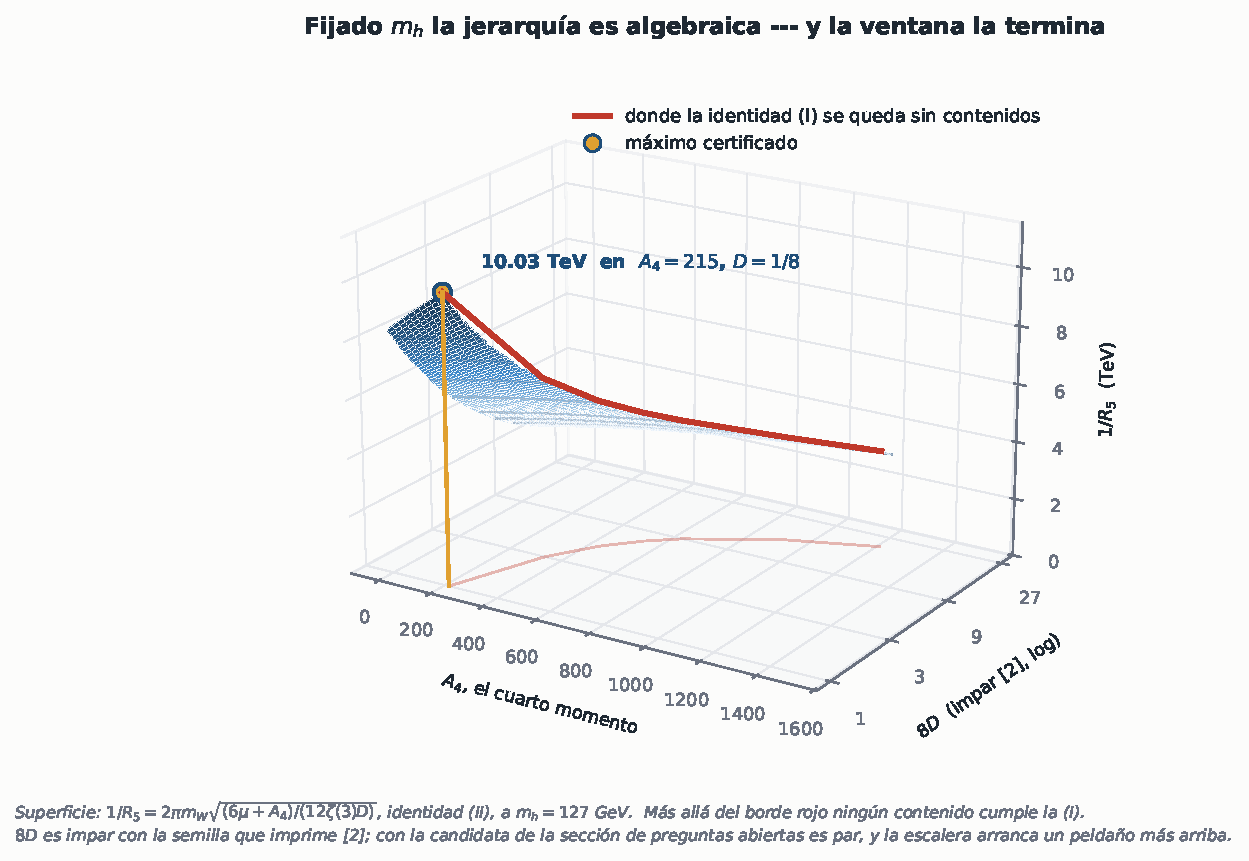
\includegraphics[width=\textwidth]{fig_surface_es.pdf}
\caption{\textbf{La geometría del techo.} Una vez fijado $m_h$, la identidad (II) convierte $1/R_5$ en una superficie explícita sobre los dos momentos cuantizados, sin minimización alguna dentro. La curva roja es donde la identidad (I) se queda sin contenidos: más allá, el retículo no puede suministrar un $G$ lo bastante pequeño. El máximo de la superficie sobre la región factible es el techo certificado, y se sienta en el menor peldaño positivo que la aritmética admite.}\label{fig:surface}
\end{figure}

\bridge{Una cota sólo vale la pena enunciarla si se puede hacer algo con ella ---y los mismos dos
enteros que la produjeron dicen además dónde, dentro de la cota, se le permite estar a la
respuesta.}

% ===================================================================
\section{Qué predice esto}\label{sec:pred}

\paragraph{Sin anclaje, y aritmético ---pero no por igual.} La congruencia
$8D-2A_4\equiv0\pmod6$ es propiedad del retículo de materia y de nada más: sin normalización, sin
orden de lazos, sin esquema, y sin sector gauge tampoco. La \emph{paridad} del $8D$ total es harina de otro costal: la fija el punto base gauge, y de cuál sea ese punto base trata la \S\ref{sec:open}. Las
dos siguen siendo pruebas que un lector puede pasar al artículo de otro en un minuto; sólo la
primera es una prueba del contenido y no de la semilla. Sus propias cinco filas pasan las dos.

\paragraph{Una correlación, no dos números.} $\amin$ y $m_h$ son funciones de los mismos dos
momentos, así que no son datos independientes. Fijar $m_h$ al valor medido \emph{determina} $1/R_5$ a
partir del contenido mediante la (II), sin minimización ---que es lo que hace computable el techo
siquiera.

\paragraph{Y la escala de Kaluza-Klein no es un continuo: se sienta en un peine aritmético.} Cruce
la (II) con el Teorema~\ref{thm:mod6} y sale algo que ninguno de los dos dice por separado.
Escribiendo $k=8D$ y $M_{\mathrm{KK}}=1/R_5=2m_W/\amin$, la (II) se lee
\begin{equation}\label{eq:comb}
  M_{\mathrm{KK}}^{2}\;=\;\frac{8\pi^2m_W^2}{3\zeta(3)}\;\frac{6\mu+A_4}{k}\,,
\end{equation}
y el Teorema~\ref{thm:mod6} fija $A_4$ módulo tres una vez fijado $k$, de modo que a $k$ fijo y
$m_h$ fija los $A_4$ admisibles avanzan de tres en tres y
\begin{equation}\label{eq:comb2}
  M_{n+1}^{2}-M_{n}^{2}\;=\;\frac{8\pi^2m_W^2}{\zeta(3)\,k}\,,
\end{equation}
con independencia del contenido y de la masa del Higgs. \textbf{La cantidad exactamente espaciada
es $M^2$, no $M$}, y un espaciado en masa es $\Delta M=\Delta M^2/2M$, de modo que no significa nada
sin decir en qué $M$ ---y cada peldaño tiene su propio techo, así que citarlos todos a una misma
masa es citar a casi todos donde no llegan. En $k=1$ el paso son $0.42$~TeV$^2$, que en el techo
propio de ese peldaño, $10$~TeV, son $21$~GeV de masa; en $k=11$ el paso son $0.039$~TeV$^2$ y el
techo son $3.97$~TeV, luego $4.9$~GeV. La afirmación es
\emph{necesaria y no suficiente} ---todo contenido realizable cae en un diente, no todo diente
aloja un contenido--- y la \emph{posición} del peine arrastra el residuo del anclaje y la elección de
$g_4$, mientras que su \emph{espaciado} no, por ser aritmético. Leída como prueba resulta insólita:
dados $m_h$, $m_W$, $g_4$ y una candidata a resonancia de Kaluza-Klein, cabe preguntar si algún par
admisible $(k,A_4)$ la reproduce. \textbf{Cuáles son admisibles es cosa de la semilla y no del
retículo}: con la que \cite{KM25} imprimen la prueba dice $k$ impar, $A_4\in\ZZ$ y
$A_4+k\equiv0\pmod3$, mientras que con la candidata $k$ es par y $A_4\in\ZZ+\tfrac12$. Lo que
sobrevive a las dos es el Teorema~\ref{thm:mod6} escrito de modo que toda entrada sea entera con
las dos semillas ---$A_4$ es semientero con la candidata, $2A_4$ no---, o sea
$k-2A_4\equiv3\pmod6$ con $(2A_4,k)\in\ZZ^2$.
El espaciado es del retículo de materia y el desplazamiento es del coset afín, que es la misma
separación sobre la que gira la \S\ref{sec:open}. Verificado contra la fila del
certificado de la \S\ref{sec:ceiling} en \texttt{crossed\_\allowbreak equations.py}.

\paragraph{Y el techo tiene dientes de colisionador.} Una
cota sobre $1/R_5$ es una cota sobre una escala de compactificación y no sobre la masa de una
resonancia concreta. Las ecs.~(18)--(19) de \cite{KM25} desarrollan las componentes de paridad
mixta en $\cos\bigl((n+\tfrac12)x_5/R_5\bigr)$, así que esas torres tienen modos semienteros y su
estado más ligero se sitúa en $1/(2R_5)$, mientras que los bosones gauge no rotos conservan niveles
enteros $n/R_5$. Cuál de ellos acota una búsqueda dada, con qué acoplo a los quarks de los puntos
fijos y con qué anchura, lo fijan esas mismas paridades y se deriva en la \S\ref{sec:collider}; la
respuesta corta es que la torre semientera es un singlete de color y que el único estado coloreado
por debajo de la escala de Planck es la torre del gluón en $n/R_5$.
Arrastrando el residuo del anclaje de la \S\ref{sec:setting}:

\begin{center}\small
\rowcolors{2}{white}{softgrey}
\begin{tabular}{lrr}
\toprule
\rowcolor{hdrblue!10} & nuestra normalización & $\times$ el mayor cociente medido\\
\midrule
contenido de su tamaño ($\le6$ multipletes) & $2.18$~TeV & $4.53$~TeV\\
techo sobre \emph{todos} los contenidos & $10.03$~TeV & $20.82$~TeV$^{\dagger}$\\
\rowcolor{amber!14}techo con el vacío obligado a ser el verdadero & $9.22$~TeV & $19.14$~TeV$^{\dagger}$\\
techo si hay que costear el escape & $3.97$~TeV & $8.24$~TeV$^{\dagger}$\\
\bottomrule
\end{tabular}
\end{center}

\noindent A la masa que el Higgs tiene de verdad, en vez de al tope de la ventana de \cite{KM25},
la fila resaltada dice $9.09$~TeV ---la \eqref{eq:ceilingmeasured}, y el número que hay que citar a
la masa física, con las dos mismas salvedades que toda escala del lado teórico de aquí. Para ella
no se arrastra la columna de la derecha, que ya
es una extrapolación.

\noindent La fila resaltada es la física: la de encima admite contenidos cuyo punto electrodébil es
estacionario sin ser el mínimo, y la \S\ref{sec:ceiling} muestra que el contenido que la satura es
justo de ésos. Los $10.03$ se conservan porque son la cota que el certificado demuestra para
contenido arbitrario, y porque la diferencia entre las dos filas ---ochocientos GeV--- es lo que
vale una sola condición física.

\noindent$^{\dagger}$\emph{Extrapolaciones, no cotas.} La columna de la derecha multiplica por
$2.076$, el mayor cociente medido sobre las cinco filas publicadas. Eso es legítimo para la primera
fila, cuyos contenidos son del tamaño de los suyos y caen dentro del rango anclado. No lo es para
las otras dos: por la \S\ref{sec:setting} el cociente es una tendencia y no dispersión, y los dos
techos quedan fuera del rango que la mide ---el primero en $D$ ($1/8$ frente a $[1.125,3.625]$), el
segundo en $A_4$ ($727$ frente a $[189,271]$). La tendencia crece hacia el primero de esos rincones,
de modo que $20.8$ es, si acaso, una subestimación de dónde caería el techo reescalado; pero es una
extrapolación de
cinco puntos, y aquí queda escrita como tal.

\noindent Frente a las exclusiones publicadas ---un gluón de Kaluza-Klein por debajo de unos
$4$~TeV, un $Z'$ secuencial por debajo de unos $5$~TeV--- el rincón de contenido pequeño de la clase,
que es el rincón que puebla su Tabla~1, está ya desfavorecido, y eso es consecuencia de la forma
cerrada y no de ninguna medida nueva. El techo tapa entonces la clase entera. Y la cota del escape
de \eqref{eq:escapeceiling} muerde más fuerte: $3.97$~TeV cae en una región a la que los datos de
dijets son muy sensibles, y el reescalado que la subiría a $8.24$~TeV es la extrapolación señalada
arriba, no una cota, así que la sensibilidad no se esquiva apelando a él. \textbf{Y el recast ya
está hecho, que es lo que pone un número al otro lado.} No podía tomarse de los límites genéricos de
gluón de Kaluza-Klein citados arriba ---ésos son para una resonancia \emph{estrecha}, mientras que
la \S\ref{sec:collider} deriva la anchura propia de este objeto,
$\Gamma(G^{(n)}\!\to q\bar q)/M_n\simeq0.16$, y el canal $s$ necesitaría además
$\mathrm{BR}(G_1\to jj)$, que el modelo no fija---. El factor de forma espacial \eqref{eq:resum}
no necesita ninguna de las dos, y llevado a través de la covarianza publicada de
\cite{CMSangular} da una sensibilidad nominal de recast de $1/R_5>10.86$~TeV, que sube a
$13.75$~TeV en el rango de masas que \cite{CMSangular} usa para sus propias interacciones de
contacto. \textbf{Así que la rama que además puede pagar el escape de la desintegración del protón de
la Parte~VI, en $3.97$~TeV, queda un factor tres por debajo de donde este recast pierde
sensibilidad.} La \S\ref{sec:collider} dice cómo, por qué eso todavía no es la palabra
\emph{excluida}, y qué la haría serlo.

\begin{keyeq}
La predicción está acotada \emph{por arriba}, que es la dirección útil: \textbf{el modelo no puede
replegarse a escalas más altas añadiendo materia.} Añadir materia sube $A_4$, y un $A_4$ mayor sube
$1/R_5$ sólo hasta que la ventana del Higgs se lo corta ---que es precisamente lo que mide el
programa entero. Un análisis con sensibilidad demostrada a \emph{esta} torre en todo el rango de
masas que el álgebra permite podría por tanto poner a prueba la clase de tres peldaños ---una
afirmación más débil que decir que la zanja una máquina de tal o cual energía de haz, y la
correcta: la \S\ref{sec:collider} dice qué resonancia, por qué el alcance y la energía de haz no
son el mismo número, y qué queda todavía entre una sensibilidad y una exclusión.
\end{keyeq}

\paragraph{Una predicción dentro del marco de otros.} La ecuación~\eqref{eq:valuebound} dice que el
criterio de estabilidad del orbifold de \cite{CCD24}, aplicado a este modelo, nunca queda en empate.
Es un enunciado en su lenguaje, sobre su pregunta, comprobable contra su propio código.

\bridge{Un techo sobre una escala de compactificación no es un techo sobre nada que registre un
detector. ¿Qué estado estaría acotando de verdad una búsqueda, con qué acoplo y qué anchura ---y
es algo de eso nuestro para elegirlo?}

% ===================================================================
\section{Qué estado acota una búsqueda}\label{sec:collider}

Una cota sobre $1/R_5$ es una cota sobre una escala de compactificación, no sobre la masa de
ninguna partícula concreta. Un colisionador no mide escalas de compactificación; mide resonancias,
cada una con su ritmo de producción y su anchura. Pasar de lo uno a lo otro parece exigir un
estudio fenomenológico, y no lo exige: queda fijado por las tres matrices de paridad de \cite{KM25}
y por los desarrollos en modos que se siguen de ellas, todo ello ya publicado. Esta sección los
lee.

\paragraph{La paridad que separa el color.} De las tres matrices $\ZZ_2$, la que actúa en $x_6$ es
\begin{equation}\label{eq:P6}
  P_6=\mathrm{diag}(+,+,+,-,-,-,-),
\end{equation}
la (11) de \cite{KM25}, que parte el índice heptadimensional en el triplete de color y todo lo
demás. Una componente gauge a lo largo de $E_{ij}$ lleva el \emph{producto} $P_6^{(i)}P_6^{(j)}$,
de modo que \eqref{eq:P6} tiene una consecuencia inmediata, aritmética y no dinámica:
\begin{equation}\label{eq:colourparity}
  P_6(i,j)=-1
  \quad\Longleftrightarrow\quad
  \text{exactamente uno de } i,j \text{ es un índice de color,}
\end{equation}
esto es, precisamente cuando el generador cambia el color. Hay $24$ componentes así, y no hay
ninguna componente que cambie el color con $P_6=+1$.

\begin{theorem}[el color vive en el círculo pequeño]\label{thm:colourparity}
Todo bosón gauge de \cite{KM25} que cambie el color tiene $P_6=-1$. Por sus (21)--(24) cada una de
esas componentes se desarrolla en $\sin(m x_6/R_6)$ con $m\ge1$. Por tanto su nivel más ligero está
al menos en $1/R_6$, y su función de onda \emph{se anula} en $x_6=0$.
\end{theorem}
\begin{proof}
\eqref{eq:colourparity} dice que $P_6^{(i)}P_6^{(j)}=-1$ si y sólo si uno de los índices cae en el
bloque de color, lo cual es inmediato desde \eqref{eq:P6}. Los cuatro desarrollos $P_6$-impares de
\cite{KM25}, sus (21)--(24), llevan todos $\sin(m x_6/R_6)$ y todos empiezan en $m=1$; el seno se
anula en el origen y el nivel está acotado inferiormente por el término $m=1$.
\end{proof}

\noindent Esto importa porque la p.~3 de \cite{KM25} fija $R_5\gg R_6$ y llama a $1/R_6$ un parámetro arbitrario, ``que es la escala de Planck, por
ejemplo''. El teorema~\ref{thm:colourparity}
dice entonces que los exóticos coloreados no tienen acoplo alguno a nivel árbol con los quarks de
la brana, y que en la jerarquía $R_5\gg R_6$ que el modelo pretende quedan muy fuera del alcance de
un colisionador. Ninguna de las dos cosas es que sean inobservables en principio: $1/R_6$ se
declara arbitrario y no fijo, y un $X_m$ coloreado sigue siendo un campo gauge del bulk, de modo
que el vértice $g^{(0)}X_mX_m$ lleva $\int\!\mathrm{d}x_6\,\sin^2(mx_6/R_6)\neq0$ y la producción
en pares por QCD sobrevive a la anulación del vértice de un solo $X$. Lo que el teorema elimina es
el canal directo, que es el que importa para la desintegración del protón.

\paragraph{Así que los quarks de la brana ven exactamente dos torres.} La p.~22 de \cite{KM25}
introduce los ``quarks $q_L,u_R,d_R$ como fermiones 4D en la brana del origen del espacio
compactificado $(0,0)$''. Un campo 4D allí acopla sólo a componentes cuya función de modo no se anule en ese
punto ---esto es, a componentes cuyos factores en $x_5$ \emph{y} en $x_6$ sean ambos cosenos---. De
las ocho clases de paridad sólo dos cumplen, y ambas son diagonales en color:

\begin{center}\small
\rowcolors{2}{white}{softgrey}
\begin{tabular}{llllll}
\toprule
\rowcolor{hdrblue!10} paridad & ec. & modo $x_5$ & modo $x_6$ & en $(0,0)$ & nivel más bajo\\
\midrule
$(+,+,+)$ & (17) & $\cos(nx_5/R_5)$ & $\cos(mx_6/R_6)$ & \textbf{no nulo} & $0$, luego $1/R_5$\\
$(+,+,-)$ & (18) & $\cos((n{+}\tfrac12)x_5/R_5)$ & $\cos(mx_6/R_6)$ & \textbf{no nulo} & $1/(2R_5)$\\
$(+,-,+)$ & (19) & $\sin((n{+}\tfrac12)x_5/R_5)$ & $\cos(mx_6/R_6)$ & nulo & $1/(2R_5)$\\
$(+,-,-)$ & (20) & $\sin(nx_5/R_5)$ & $\cos(mx_6/R_6)$ & nulo & $1/R_5$\\
$(-,\cdot,\cdot)$ & (21)--(24) & --- & $\sin(mx_6/R_6)$ & nulo & $\ge 1/R_6$\\
\bottomrule
\end{tabular}
\end{center}

\noindent La clase $(+,+,-)$ son exactamente las dos posiciones $(6,7)$ y $(7,6)$ ---un singlete de
color---. De modo que la torre semientera, cuyo estado más ligero está en $1/(2R_5)$ y que la
\S\ref{sec:pred} señalaba con razón como el nivel más bajo del modelo, \emph{no} es algo que una
búsqueda de dijets pueda ver; y tampoco es una predicción limpia, porque el $\langle W\rangle$ de
la (77) de \cite{KM25} actúa en el bloque $(5,7)$ y la desplaza con $\alpha$. El único objeto
coloreado por debajo de la escala de Planck es la torre del gluón.

\paragraph{Y eso responde una pregunta que \cite{KM25} dejó abierta.} Sus conclusiones dicen:
``Puesto que la masa de los bosones gauge $X$, $Y$ es pequeña en nuestro modelo, esto provoca
desintegración rápida del protón \emph{si pueden acoplarse a quarks y leptones}'', y dejan la cuestión para trabajo futuro. Por el
teorema~\ref{thm:colourparity} no pueden: los bosones $X$ e $Y$ son precisamente las componentes
que cambian el color, y su función de onda es cero en el punto fijo donde ese mismo artículo pone
los quarks. El canal de intercambio gauge lo cierra la propia asignación de paridades.

\noindent\textbf{El alcance de eso es estrecho y conviene decirlo.} Es un enunciado a nivel árbol
sobre intercambio gauge, para los quarks localizados como en la p.~22 de \cite{KM25}. No dice nada
sobre las masas de Dirac de brana que ese mismo artículo introduce en su p.~16 para levantar sus
modos cero no deseados, y \emph{no} es el escape de la Parte~VI \cite{PartVI}, que es una carga
dependiente de familia alojada en un $\rep{84}^{(+,+)}$ donado ---otro mecanismo, que ataca otro
operador---. En particular la \eqref{eq:escapeceiling} queda intacta.

\paragraph{La masa y el acoplo a quarks del colorón están fijados ---y ninguno es nuevo.} Lo fijan tres hechos, y los
tres son resultados de otros aplicados aquí, no hallados aquí. La masa: la p.~16 de
\cite{KM25} afirma que los generadores de $\su3_C$ ``conmutan con $\langle W\rangle$ con
independencia del VEV $\alpha_{\min}$'', de modo que la torre de color no recibe desplazamiento
de línea de Wilson y se sitúa exactamente en $n/R_5$. El acoplo: su (17) lleva $\sqrt2$ delante de
cada modo $(n,0)$ donde el modo cero lleva $1$, y $\cos(0)=1$, así que en la brana la razón es
$\sqrt2$ ---y es universal en sabor, porque $q_L$, $u_R$ y $d_R$ están en el mismo punto y ven la
misma función de modo---. La anchura sale entonces del resultado estándar para un octete de color,
$\Gamma(C\to q\bar q)=n_f\,\alpha_s\cot^2\theta\,M/6$, con $\cot^2\theta=2$ y $n_f=6$:

\begin{keyeq}
\begin{equation}\label{eq:coloron}
  M_n=\frac{n}{R_5},
  \qquad
  \frac{g_{G^{(n)}q\bar q}}{g_{gq\bar q}}=\sqrt2,
  \qquad
  \frac{\Gamma(G^{(n)}\!\to q\bar q)}{M_n}=2\alpha_s(M_n)\simeq0.16 .
\end{equation}
\end{keyeq}

\noindent \textbf{De quién es cada uno.} El $\sqrt2$ de un bosón gauge de Kaluza-Klein sobre un
fermión localizado en una brana, y la anchura $\Gamma_n=2\alpha_s m_n$ que lo acompaña, son de
\cite{DMN01}, cuyo lagrangiano ---campos gauge en el bulk, quarks sujetos en $y=0$ por una delta---
es estructuralmente el montaje de \cite{KM25}. El lagrangiano de octete de color y la fórmula de la
anchura son de \cite{Simmons97}; la sección eficaz de producción a orden siguiente al dominante es
de \cite{Chivukula13}; y un gluón de Kaluza-Klein confrontado con una distribución de dijets en un
modelo gauge-Higgs es de \cite{KS16}, que además señalan que $\sqrt2 g_s$ es el acoplo \emph{máximo}
disponible y arrastran un parámetro libre por debajo. Lo propio de aquí es sólo que \cite{KM25}
pone sus quarks exactamente en el punto fijo, de modo que la cota se satura en vez de suponerse
---y que la \eqref{eq:ceiling} tapa la escala por arriba, que es lo que hace que cualquiera de
estos números sea contrastable. Arrastrado por las filas de la \S\ref{sec:pred}:

\begin{center}\small
\rowcolors{2}{white}{softgrey}
\begin{tabular}{lrrrr}
\toprule
\rowcolor{hdrblue!10} & $1/R_5$ & $\alpha_s$ & $\Gamma/M$ & $\Gamma$\\
\midrule
\rowcolor{amber!14}techo a la masa del Higgs medida & $9.09$~TeV & $0.0735$ & $0.147$ & $1337$~GeV\\
techo una vez el vacío debe ser el verdadero & $9.22$~TeV & $0.0734$ & $0.147$ & $1354$~GeV\\
techo sobre \emph{todos} los contenidos & $10.03$~TeV & $0.0729$ & $0.146$ & $1463$~GeV\\
contenidos que pueden pagar el escape & $3.97$~TeV & $0.0789$ & $0.158$ & $626$~GeV\\
\bottomrule
\end{tabular}
\end{center}

\paragraph{Lo cual cambia qué puede citarse en su contra.} Una anchura de un sexto de la masa no es
una resonancia estrecha, así que el patrón estrecho de una búsqueda de dijets no acota este objeto:
los $6.6$~TeV de CMS para un axigluón o colorón estrecho con $137\,\mathrm{fb}^{-1}$
\cite{CMSdijet} son una cota sobre otra partícula. Lo que sí aplica es la cota
independiente de modelo sobre $\sigma\,B\,A$ que ese mismo análisis publica en función de la masa
\emph{y} de la anchura, leída en $\Gamma/M\simeq0.16$. La versión anterior de esta sección comparaba
la \eqref{eq:escapeceiling} con una exclusión genérica de gluón de Kaluza-Klein; la
\eqref{eq:coloron} es lo que convierte esa comparación en un enunciado sobre este modelo y no sobre
un patrón de referencia, y es la razón por la que la comparación merece hacerse.

\paragraph{Una corrección a cómo se enunciaba el alcance.} Una versión anterior de este artículo
escribía que una máquina que alcanzase $10$--$20$~TeV zanja la clase. Eso confunde la energía de un
colisionador con su alcance en masa de resonancia, y no son lo mismo: producir una resonancia de
$9$~TeV a $\sqrt s=13$~TeV exige partones con valores de $x$ donde las densidades partónicas son
despreciables. El enunciado correcto es sobre alcance en masa en el canal pertinente, y hace la
rama del escape mucho más interesante que el techo: $3.97$~TeV cae donde el Run~2 tiene
sensibilidad real, y $9.09$~TeV no.

\paragraph{La torre actúa también por debajo de la primera resonancia.} Como todo modo $(n,0)$
lleva el mismo $\sqrt2$ en $x_5=0$, integrar la torre entera da un operador de cuatro quarks en
octete de color con un coeficiente que es un número puro:
\begin{equation}\label{eq:tower}
  \sum_{n\ge1}\frac{g_n^2}{2M_n^2}
  \;=\;g_s^2R_5^2\sum_{n\ge1}\frac{1}{n^2}
  \;=\;\frac{\pi^2}{6}\,g_s^2R_5^2 ,
  \qquad\text{es decir}\qquad
  \Lambda_8=\frac{\sqrt3}{\pi\sqrt{\alpha_s}}\,\frac{1}{R_5},
\end{equation}
que vale $7.79$~TeV en la rama del escape y $18.48$~TeV en el techo a la masa medida.
\textbf{De esos dos números hay que decir dos cosas antes de que nadie los compare con una cota
publicada.} Primera, la \eqref{eq:tower} es el término principal de un desarrollo en
$\hat s/M_1^2$, y los datos de dijets que lo probarían están en $M_{jj}\sim2$--$8$~TeV ---que cae
\emph{sobre} la torre cuando $1/R_5=3.97$~TeV, y no por debajo de ella---. Ahí el operador de contacto es el
objeto equivocado, y el enunciado exacto a nivel árbol es sustituir el propagador del gluón por
$1/q^2+\sum_n 2/(q^2-M_n^2+iM_n\Gamma_n)$ de \cite{DMN01}, que es lo que evalúa
\texttt{kk\_\allowbreak dijet\_\allowbreak lo.py}. \textbf{Segunda, y sustituye a una corrección
que una versión anterior de esta sección llevaba}: ese propagador no hay que truncarlo en los
canales espaciales, y ahí no debe llevar anchura. Para $t<0$ cada modo queda por debajo de su
umbral de dos partones, así que la autoenergía no tiene parte absortiva y el propagador es real; y
con todos los $c_n$ iguales ---que es el Teorema~\ref{thm:colourparity} junto con la localización
de los quarks en el punto fijo de \cite{KM25}, y es lo que hace que la suma sea
$\sum_n(n^2+a^2)^{-1}$ y no una cualquiera--- el desarrollo de Euler la hace en forma cerrada. Con
$a=R_5\sqrt{-t}$,
\begin{keyeq}
\begin{equation}\label{eq:resum}
  \frac{1}{q^2}+\sum_{n\ge1}\frac{2}{q^2-n^2/R_5^2}\;=\;\frac{\mathcal F(q^2)}{q^2}\,,\qquad
  \mathcal F(q^2)=
  \begin{cases}
    \pi a\coth(\pi a)\,, & a=R_5\sqrt{-q^2}\,,\quad q^2<0\,,\\[2pt]
    \pi b\cot(\pi b)\,,  & b=R_5\sqrt{q^2}\,,\quad q^2>0\,.
  \end{cases}
\end{equation}
\end{keyeq}
\noindent de modo que toda la torre coloreada es un solo \emph{factor de forma} sobre el propagador
del gluón. La resumación es estándar ---así se escribe un propagador de brana a brana, y la
identidad es de Euler---; lo específico de aquí es que el $\sqrt2$ universal la hace posible. Se
siguen tres cosas de golpe. Su desarrollo $\pi a\coth\pi a=1+\pi^2a^2/3-\pi^4a^4/45+\cdots$
devuelve $-\pi^2R_5^2/3$, que es la \eqref{eq:tower}: el operador de contacto es el primer término
de la \eqref{eq:resum} y no un enunciado aparte. En un subproceso con sólo intercambio en $t$ el
cociente a nivel partónico es exactamente $\mathcal F^2$, y con $|t|=M_{jj}^2/(1+\chi)$ eso es una
forma cerrada en las dos variables en que la medida está binada. Y \emph{no depende de}
$\mathrm{BR}(G_n\to jj)$, porque no se produce ni se desintegra nada ---que es justo lo único que
el modelo no da, más abajo. \textbf{Queda por tanto retirada la corrección del $2.55\%$ a
$\Lambda_8$ que aquí figuraba}: venía de meter un $iM_n\Gamma_n$ fijo donde no hay parte absortiva
que meter, y el delator es que el desplazamiento no se apaga cuando $t\to0$ sino que tiende a
$1/(1+(2\alpha_s)^2)$, cosa que ninguna autoenergía bajo umbral puede hacer. El $\pi^2/6$ a
anchura cero es el coeficiente correcto, no una aproximación a otro mejor. Medido en
\texttt{kk\_\allowbreak resummation.py}.

\noindent\textbf{Y la segunda línea de la \eqref{eq:resum} colapsa esta sección en un
solo enunciado.} Nada en la suma exigía $q^2<0$; eso era sólo donde podía quitarse la
anchura. El mismo desarrollo continúa al lado temporal por $\coth(ix)=-i\cot x$, de modo que
una sola función analítica cubre toda la torre a nivel árbol. Entonces las tres cosas que
esta sección venía diciendo por separado son tres regiones de ella. El operador de contacto
\eqref{eq:tower} es su desarrollo alrededor de $b=0$. La distorsión angular de la
Figura~\ref{fig:tower} es su rama espacial. Y \emph{las resonancias son los polos del
cotangente}, en $b=1,2,3,\dots$, es decir $\sqrt{q^2}=n/R_5$ ---no se meten a mano ni hace
falta suma truncada ninguna para encontrarlos; son donde la forma cerrada diverge, y son
exactamente y sólo ahí donde una anchura debe sustituir al polo. Así que las amplitudes quedan
$\mathcal M_{qq\to qq}=\mathcal M_{\mathrm{QCD}}[\mathcal F(t),\mathcal F(u)]$ y
$\mathcal M_{q\bar q\to q\bar q}=\mathcal M_{\mathrm{QCD}}[\mathcal F(s),\mathcal F(t)]$, y la
anchura entra en exactamente uno de los cuatro argumentos. Las dos ramas comprobadas contra
la suma en \texttt{kk\_\allowbreak resummation.py}.

\noindent\textbf{Y el segundo círculo sí es sensible al UV, así que lo que hay que citar es su
coeficiente y no su ausencia.} Una versión anterior de este párrafo decía que la divergencia
logarítmica que uno temería de una brana de codimensión dos ``nunca se enciende''. Sí se
enciende: una torre bidimensional es logarítmicamente sensible al corte y ninguna jerarquía
quita eso. Lo que la jerarquía suprime es el coeficiente, y la misma identidad de Euler lo da.
Sumando primero en $n$ a $m$ fija, $\sum_{n\in\ZZ}(n^2/R_5^2+m^2/R_6^2)^{-1}=\pi R_5(R_6/m)
\coth(\pi mR_5/R_6)\to\pi R_5R_6/m$ para $R_5\gg R_6$, de modo que
\begin{equation}\label{eq:codim2}
  \frac{\Delta C_{m\ge1}}{C_{m=0}}\;=\;\frac{6}{\pi}\,\frac{R_6}{R_5}\,\ln(\Lambda R_6)\,,
\end{equation}
logarítmica en el corte y con una potencia de $R_6/R_5$ delante ---un $1.3\%$ con
$R_5/R_6=10^3$ y un corte una década por encima de $1/R_6$, y mucho menos al $1/R_6$ que
contempla la p.~3 de \cite{KM25}---. Verificada contra la suma doble directa en
\texttt{kk\_\allowbreak resummation.py}. Ésta es una predicción
colectiva de la torre y no exige resolver ninguna resonancia; no puede, en cambio, compararse
directamente con las escalas de composición publicadas, cuyo operador tiene otra estructura de
color y de quiralidad.

\paragraph{Y un número que el modelo no suministra.} La p.~16 de \cite{KM25} levanta sus modos cero
no deseados introduciendo ``fermiones 4D conjugados de las representaciones y cargas de los
fermiones sin masa, y sus términos de masa de Dirac en los puntos fijos'', y no fija esas masas. Si algún exótico
coloreado queda por debajo de $M/2$, se abre $G^{(1)}\to\Psi\bar\Psi$, la anchura crece y
$\mathrm{BR}(G^{(1)}\to jj)$ baja en una cantidad que nada de aquí determina. Así que
\begin{equation}\label{eq:brhole}
  \mathrm{BR}(G^{(1)}\to jj)=1 \quad\text{si todo exótico coloreado está por encima de } M/2,
\end{equation}
y menos en caso contrario. Esa única incógnita es lo que se interpone entre el techo aritmético y
una exclusión propia del modelo, y una cota citada sin ella sería independiente de modelo sólo en
apariencia. Se dice aquí, en lugar de disimularla.

\paragraph{Y esa incógnita apunta a una medida distinta de la que uno esperaría.} Una búsqueda de
resonancia busca un pico, y un pico es sólo el primer peldaño de la \eqref{eq:coloron} ---así que su
ritmo depende justamente de la razón de desintegración que la \eqref{eq:brhole} deja sin fijar---. Pero los
quarks de \cite{KM25} están en un punto, así que ven \emph{todos} los peldaños con el mismo
$\sqrt2$, y lo que hace la torre entera no es añadir un pico, sino sustituir el propagador del gluón por
$1/q^2+\sum_n2/(q^2-M_n^2+iM_n\Gamma_n)$ ---en \emph{todos} los canales, $t$ y $u$ además de
$s$, que es como lo escriben \cite{DMN01}---. Muy por debajo del primer peldaño el cambio es una
constante, $-\tfrac{\pi^2}{3}R_5^2$, así que el cambio \emph{relativo} crece con $|q^2|$; y a masa
de dijet fija $|t|=M_{jj}^2/(1+\chi)$ es máximo a $\chi$ pequeño. El efecto es por tanto central, y
el observable es la distribución angular y no el espectro de masas.

\noindent Y existe una medida hecha justo para eso. \cite{CMSangular} publica
$\chi_{\mathrm{dijet}}$ con $138\,\mathrm{fb}^{-1}$ \emph{corregida de efectos del detector} y
comparada con QCD a orden siguiente al siguiente del dominante, citando una incertidumbre teórica
total del $3.5\%$ en su bin de masa $3.0$--$3.6$~TeV. Al estar desplegada, puede confrontarse
directamente con un cálculo, sin simular el detector. Evaluar la \eqref{eq:resum} en el bin de
$\chi$ más bajo de ese mismo rango de masas da un cociente respecto a QCD de $1.36$ en el techo a
la masa medida y de $3.16$ en la rama del escape, frente al $1.3$ y al $3.4$ que devuelve ahí
mismo el cálculo de todos los canales de \texttt{kk\_\allowbreak dijet\_\allowbreak lo.py} ---los
dos concuerdan al uno y medio por ciento donde deben;
la Figura~\ref{fig:tower} dibuja la forma entera, y la forma es lo que importa
---la desviación se concentra a $\chi$ pequeño y se apaga hacia $\chi=16$, que es lo que un
análisis angular está hecho para ver y una búsqueda en el espectro de masas no. Son números partónicos y por tanto una sobreestimación ---los subprocesos
iniciados por gluones no ven la torre, por el mismo argumento de conservación de cinco-momento de
\cite{DMN01} que la excluye de $q\bar q\to gg$, y la diluyen---. La comparación con el $3.5\%$
tampoco es una significancia, y encima no es el $3.5\%$ correcto en todos los bins: esa cifra es
la incertidumbre teórica total de \cite{CMSangular} en el bin $3.0$--$3.6$~TeV y nada más, y por
encima de $7$~TeV la suya es del $12.2\%$ ---escala, $m_{jj}$ frente a $\langle p_T\rangle$,
densidades partónicas y el generador NNLO, en ese orden de tamaño---. Una deformación que crece a
lo largo de los bins de masa hay que leerla, por tanto, contra una incertidumbre que crece con
ella, y contra las correlaciones entre bins: que es lo que hace el recast de abajo y lo que el
tamaño de un efecto partónico no puede hacer.

\begin{figure}[t]
\centering
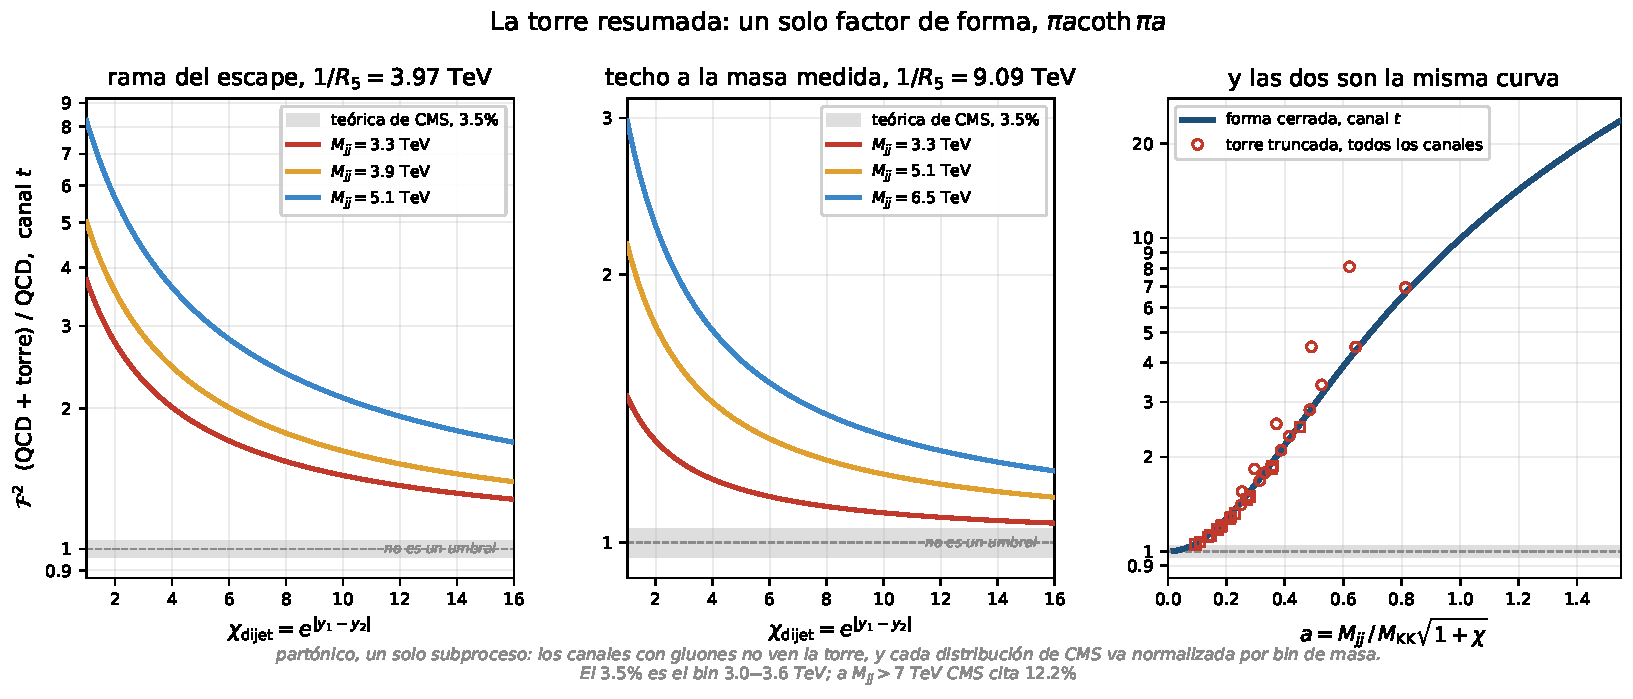
\includegraphics[width=\textwidth]{fig_tower_es.pdf}
\caption{\textbf{Por qué la distribución angular y no el espectro de masas ---y es una sola
función.} El cociente exacto de canal-$t$, $\mathcal F^2$ de la \eqref{eq:resum}, sin truncar, sin
anchura y sin $\mathrm{BR}(G_n\to jj)$. A masa de dijet fija $|t|=M_{jj}^2/(1+\chi)$, así que el
efecto es máximo donde $\chi$ es mínimo, que es justo donde el QCD de canal-$t$ es más débil.
\emph{Izquierda:} la rama que además puede pagar el escape de la desintegración del protón de la
Parte~VI. \emph{Centro:} la clase entera, con el techo a la masa medida del Higgs.
\emph{Derecha:} por qué las dos son la misma imagen. $\mathcal F$ ve $M_{jj}$, $\chi$ y
$M_{\mathrm{KK}}$ sólo a través de $a=M_{jj}/M_{\mathrm{KK}}\sqrt{1+\chi}$, de modo que cada curva
de los otros dos paneles \emph{es} $(\pi a\coth\pi a)^2$ y todas colapsan sobre una línea. Los
marcadores huecos son el cálculo superado de \texttt{kk\_\allowbreak dijet\_\allowbreak lo.py}
---torre truncada, anchuras puestas---, que se encuentra con la forma cerrada al $1.4\%$ lejos de
la torre y sólo se separa por arriba donde se abre el canal $s$; esa separación es exactamente la
parte que $\mathcal F^2$ no describe, y está dibujada en vez de contada. La banda gris es el
$3.5\%$ de incertidumbre teórica total que \cite{CMSangular} cita para su
$\chi_{\mathrm{dijet}}$ normalizada en el bin $3.0$--$3.6$~TeV ---dibujada para dar escala al
eje vertical, \textbf{no como umbral de exclusión}, que exigiría la verosimilitud completa sobre
bins correlacionados---. \textbf{Y las curvas son una sobreestimación}: son un solo subproceso a
nivel partónico, los iniciados por gluones no ven la torre en absoluto por el mismo argumento de
cinco-momento que la excluye de $q\bar q\to gg$, y cada distribución de CMS va normalizada por bin
de masa. Lo que la imagen establece es el tamaño y la forma ---lo cual es una razón para hacer el
recast, no el resultado de haberlo hecho---. Dibujada por
\texttt{make\_\allowbreak fig\_\allowbreak tower.py}.}\label{fig:tower}
\end{figure}

\noindent\textbf{Y la cota publicada no es la que hay que leer.} Los escenarios de interacción de
contacto de \cite{CMSangular} se declaran de acoplos en singlete de color entre quarks, mientras
que el operador de la torre es un octete de color, y los dos interfieren con QCD de forma
distinta. El octete lleva el flujo de color del intercambio de un gluón, así que en el canal $t$
interfiere a plena fuerza y el singlete no, por $\mathrm{Tr}\,T^a=0$. Esa contracción no es toda
la historia: para quarks \emph{idénticos} los términos cruzados $t$--$u$ restituyen la
interferencia del singlete, y allí su peso de color es el triple que el del octete. Ambas cosas
están verificadas con generadores explícitos en
\texttt{colour\_\allowbreak octet\_\allowbreak recast.py}, y la comprobación más simple no
necesita esa álgebra: \cite{CMSangular} cita $17$~TeV para interferencia destructiva y $37$~TeV
para constructiva, y una interferencia nula no podría hacer que la cota dependiera del signo. Así
que cuál de los dos operadores acota más un conjunto de datos dado no se decide con factores de
color: depende de la composición en sabores de la muestra. Lo que sí se sigue es que la escala
publicada no se puede trasladar sin más. Traducirla exige un cálculo, no un reescalado, y aquí
no se acomete.

\paragraph{El recast, y qué número suyo puede citarse.} \cite{CMSangular} publica la distribución
desplegada de $\chi_{\mathrm{dijet}}$ en siete bins de masa junto con una matriz de correlación
$77\times77$ y su propia predicción QCD NNLO + EW NLO en \emph{las dos} elecciones de escala, de
modo que la línea base del Modelo Estándar es suya y sólo la deformación relativa es nuestra. La
deformación es la \eqref{eq:resum} en $t$ y $u$ solamente ---sin anchura, sin
$\mathrm{BR}(G_n\to jj)$--- convolucionada con densidades partónicas sobre todos los subprocesos, y
ajustada con la elección de escala perfilada entre sus dos columnas como \emph{nuisance}, porque su
propia tensión por debajo de $4.8$~TeV se mueve entre ellas. Antes de leer el ajuste se comprueban
tres cosas. La capa hadrónica reproduce la interferencia de octete de color a orden más bajo de
CIJET al $0.2\%$ bin a bin, en absoluto y en picobarns, sobre un emparejamiento sin factor libre.
La propia NNLO de \cite{CMSangular} pasada por este $\chi^2$ da $\chi^2/\mathrm{ndf}=0.81$. Y,
apuntada al límite de interacción de contacto publicado para el operador estándar de color singlete
---y corrida sobre el rango de masas en el que ellos lo fijan, $M_{jj}>3.6$~TeV, que no son los
siete bins---, la maquinaria devuelve $17.5$ frente a sus $17$~TeV y $29.5$ frente a sus $37$~TeV.
Sobre los siete devuelve $20.5$ y $25.5$, y la diferencia es justo el asunto: una prueba de cierre
tiene que cerrar sobre la selección sobre la que cierra.

\noindent\textbf{El estadístico, escrito, porque un límite cuyo $\chi^2$ sólo está en el código no
es reproducible desde el artículo.} Sea $d$ el vector de los $77$ valores desplegados, en siete
bloques de masa $B_m$ de tamaños $(12,12,12,12,12,12,5)$, y sea
\begin{equation}\label{eq:chisq}
\begin{aligned}
  t_i(M,a)\;&=\;\mathcal N_m\Big[(1-a)\,T_i^{\mu=m_{jj}}
             +a\,T_i^{\mu=\langle p_T\rangle}\Big]\big[1+\delta_i(M)\big],\\[2pt]
  \chi^2(M)\;&=\;\min_{a\in[0,1]}\;r^{\mathsf T}C^{-1}r\,,\qquad r=d-t(M,a)\,,
\end{aligned}
\end{equation}
con $\delta_i(M)$ la deformación de la torre de la \eqref{eq:resum} en $t$ y $u$, y $\mathcal N_m$
renormalizando cada bloque de masa a área unidad, como está la medida. El \emph{nuisance} $a$
interpola linealmente entre las dos elecciones de escala publicadas por \cite{CMSangular} y se
perfila minimizando, \emph{sin} término de penalización: es una elección entre dos columnas suyas y
no un parámetro medido, así que ponerle una gaussiana sería inventarla. El número que se cita es la
$M$ en la que $\chi^2(M)-\chi^2_{\mathrm{SM}}$ cruza $3.84$, con $a$ vuelto a perfilar en cada $M$.

\noindent\textbf{Eso es un criterio referenciado al Modelo Estándar y no el punto del $95\%$ de
Wilks, y aquí la diferencia no es académica.} Wilks mide $\Delta\chi^2$ desde el \emph{mínimo}, que
coincide con $\chi^2_{\mathrm{SM}}$ sólo si el Modelo Estándar es el mejor ajuste ---y no lo es---.
Sobre los siete bins el $\chi^2$ toca fondo en $58.46$ en $1/R_5=16.0$~TeV frente a $62.57$ sin
torre ninguna: \textbf{los datos prefieren débilmente una torre finita}, por $\Delta\chi^2=4.12$.
Eso son $2.0\,\sigma$ nominales para un grado de libertad y hay que leerlo como casi nada, por una
razón que da el mismo barrido: al restringir a $M_{jj}>3.6$~TeV, que quita el bin de
$3.0$--$3.6$~TeV, la preferencia se desploma a $\Delta\chi^2=0.29$. \emph{La preferencia es el
exceso local de $2.0\,\sigma$ de \cite{CMSangular} en ese bin visto a través de nuestra plantilla,
no información que añada este recast.} Aquí no hay corrección de \emph{look-elsewhere}, ni
verosimilitud a nivel de detector, y la frontera $\theta=1/M^2\ge0$ hace que la distribución
asintótica sea una mezcla de Chernoff y no una $\chi^2_1$; damos el número porque esconderlo sería
peor, y no reclamamos nada de él.

\noindent\textbf{Así que el criterio se varía en vez de defenderse}, y lo que el lector debe mirar
es la dispersión:
\begin{center}\small
\rowcolors{2}{white}{softgrey}
\begin{tabular}{llll r}
\toprule
\rowcolor{hdrblue!10}qué se varía & puntos & covarianza & criterio & $1/R_5$ [TeV]\\
\midrule
--- (el punto de partida) & $70$ & $C$ cruda & $\Delta\chi^2_{\mathrm{SM}}=3.84$ & $11.20$\\
la referencia del $\Delta\chi^2$ & $70$ & $C$ cruda & $\Delta\chi^2_{\min}=3.84$ & $12.18$\\
referencia y unilateralidad & $70$ & $C$ cruda & $\Delta\chi^2_{\min}=2.71$ & $12.60$\\
escala perfilada \emph{discretamente} & $70$ & $C$ cruda & $\Delta\chi^2_{\mathrm{SM}}=3.84$ & $11.19$\\
normalización proyectada fuera & $70$ & $JCJ^{\mathsf T}$ & $\Delta\chi^2_{\mathrm{SM}}=3.84$ & $11.29$\\
NNPDF3.1 \cite{NNPDF31}, la base de \cite{CMSangular} & $70$ & $C$ cruda & $\Delta\chi^2_{\mathrm{SM}}=3.84$ & $11.62$\\
CT14nlo \cite{CT14} & $70$ & $C$ cruda & $\Delta\chi^2_{\mathrm{SM}}=3.84$ & $11.46$\\
\midrule
\textbf{citado en la \eqref{eq:tulimit}} & $\mathbf{77}$ & $C$ cruda & $\Delta\chi^2_{\mathrm{SM}}=3.84$ & $\mathbf{10.86}$\\
\bottomrule
\end{tabular}
\end{center}
\noindent Las columnas importan: la dispersión \emph{no} es toda redefinición estadística. Siete de
las ocho filas se apoyan en el mismo $\chi^2$ de $70$ puntos y sólo difieren en qué varían; la
última deja esa elección y se queda con los $77$, que es de donde sale el $3\%$ extra. Nada en la
tabla cambia dos cosas a la vez.

\noindent Tres de esas filas contestan objeciones y no son ajustes. La discreta perfila sobre las
dos columnas de escala de \cite{CMSangular} \emph{sin} interpolar: su diferencia es mayor que la
variación de escala habitual de seis puntos, de modo que los interpolantes intermedios no son
predicciones calculadas, y un límite que se apoyara en uno de ellos habría comprado libertad en vez
de medirla. Da $11.19$ frente a $11.20$, así que el \emph{nuisance} continuo no compra nada y queda
validado empíricamente. Las dos de densidades partónicas contestan que CT10nlo no es la base de
\cite{CMSangular} y que a $M_{jj}$ de $5$ a $8$~TeV estamos en $x$ alto, donde la mezcla
$uu:ud:dd:qg:gg$ depende del conjunto y la deformación sólo toca canales de quark:
sobre los $70$ puntos de la tabla, NNPDF3.1 da $11.62$~TeV y CT14nlo $11.46$ frente a los $11.20$
de CT10nlo ---\textbf{una dispersión del $3.7\%$, con CT10nlo el más débil de los tres}---.
\textbf{Y la misma comparación repetida en la configuración que de verdad produce la
\eqref{eq:tulimit}} ---los $77$ puntos--- da $11.27$, $11.11$ y $10.86$: la misma dispersión del
$3.7\%$, el mismo orden, CT10nlo otra vez el más débil. Así que quedarse en CT10nlo es lo
conservador en las dos, y el sistemático no depende de en cuál de los dos $\chi^2$ se haga la
comparación. \emph{Dos versiones anteriores de esta frase erraron ese número en direcciones
opuestas, las dos por comparar entre configuraciones: primero $3.8\%$, que era NNPDF3.1 a $70$
puntos contra los $10.86$ citados a $77$; y luego «$1.4\%$», de una mezcla de ambas. Citado de
forma consistente es $3.7\%$ en las dos.} CT10nlo se mantiene
además en el control contra CIJET, porque es el conjunto con el que se generó su rejilla y un
control corrido con otro no sería un control. La fila proyectada se explica más abajo. Todos los
criterios caen por encima del $10.86$~TeV citado, que es por tanto el más débil de ellos y el que
puede llevarse sin riesgo.

\noindent\textbf{Y ese $3.7\%$ es la dispersión \emph{entre} ajustes, no la incertidumbre de lo que
suponen.} Los tres conjuntos están ajustados a datos solapados bajo la misma hipótesis ---que el
protón no tiene subestructura a estas escalas--- y toda la sensibilidad de este recast se sitúa en
$x$ alto y $M_{jj}$ alto, que es donde esa hipótesis está menos constreñida y donde una densidad
partónica mal modelada y un operador de contacto de cuatro quarks producen la \emph{misma} firma.
Esa degeneración es la razón de que las búsquedas de subestructura sean difíciles, y no se cubre
variando el conjunto. No mueve la \eqref{eq:tulimit} ---nada de aquí puede decir cuánto la
movería--- pero quien lea debe saber que es un suelo bajo el sistemático y no algo que las tres
filas de arriba hayan medido.

\noindent De $C=\sigma\sigma^{\mathsf T}\!\circ R$ hay tres hechos medidos y no supuestos, y uno de
ellos corrige algo que afirmamos antes. $C$ tiene rango \emph{completo} $77$ y número de condición
$1.2\times10^4$: no se usa ni hace falta ninguna pseudoinversa. Los datos sí cumplen la restricción
de área unidad bloque a bloque, a $2\times10^{-5}$, \emph{pero $C$ no lo sabe}: sobre la dirección
de la restricción $w$ (las anchuras de los bins dentro de un bloque), $w^{\mathsf T}Cw$ va de
$0.13$ a $0.83$ de la escala del propio bloque en vez de anularse, así que la matriz publicada no
es la covarianza de la distribución normalizada sola. Una versión anterior de este trabajo
descartaba el último bin de cada bloque y lo justificaba como el remedio para una matriz singular;
esa justificación era falsa, y el descarte es una \emph{elección}. Así que se hace de las dos
maneras: sobre $70$ puntos el ajuste da $11.20$~TeV y sobre los $77$ da $10.86$~TeV, una
dispersión del $3.2\%$, y lo que se cita es el más débil. Sobre el rango de masas de contacto de
\cite{CMSangular} esos dos dan $13.95$ y $14.10$~TeV, una dispersión del $1.1\%$ ---ahí la lectura
más débil no es ninguna de las dos sino la covarianza proyectada de más abajo, $13.75$~TeV, y por
eso es el número que se cita para esa selección.

\noindent\textbf{Y ese rango completo tiene una explicación documental que es además la objeción
más afilada que se le puede hacer a este ajuste, así que va con las palabras del propio registro.}
El registro de \textsc{hepdata} describe la matriz como ``the correlation matrix of the maximum
likelihood estimators of the signal strength modifiers'', obtenida ``after the fit to the data''
---\emph{no} como la covarianza de los puntos desplegados normalizados---. Si la normalización a
área unidad se aplica \emph{después} de ese ajuste, entonces $d_i=x_i/\sum_j w_jx_j$ mezcla bins y
la covarianza de $d$ es $JCJ^{\mathsf T}$ con $J_{ij}=\delta_{ij}-d_iw_j$, que sí tiene la
dirección de la restricción como modo nulo exacto ---de modo que para esa fila, y sólo para ella,
se quita un bin por bloque normalizado y el $\chi^2$ se evalúa sobre la representación no singular
de $70$ dimensiones que queda. Tampoco ahí se usa pseudoinversa: sobre la matriz cruda porque no
hace falta, y aquí porque la dirección singular se proyecta fuera por construcción en vez de
invertirse a través de ella. Un lector tiene derecho a preguntar por qué puede usarse
$\sigma_i\sigma_jR_{ij}$ si los dos objetos pueden vivir en parametrizaciones distintas, y no
podemos zanjarlo desde el registro: no está documentado ni en un sentido ni en otro. Lo que sí
puede hacerse es calcular el límite \emph{bajo la lectura desfavorable} y ver si la pregunta tiene
alguna fuerza numérica. No la tiene: por $JCJ^{\mathsf T}$ el límite es $11.29$~TeV frente a los
$11.20$ de la matriz cruda, ocho partes en mil, y en la dirección que lo refuerza. \textbf{La
objeción es real y su consecuencia está por debajo del uno por ciento}, que es mejor respuesta que
un argumento. El
resultado es
\begin{equation}\label{eq:tulimit}
  \frac{1}{R_5}\;>\;10.86\ \text{TeV}\,,
\end{equation}
y $13.75$~TeV en el rango de masas al que \cite{CMSangular} restringe su propio límite de
interacciones de contacto, $M_{jj}>3.6$~TeV. Que el número \emph{suba} al quitar el bin de
$3.0$--$3.6$~TeV merece decirse: ese bin lleva su mayor exceso local, $2.0\sigma$, en la misma
dirección en que empujaría nuestra señal, de modo que el límite no se apoya en el único sitio
donde los datos están menos tranquilos. La Figura~\ref{fig:chi2} dibuja el perfil que esos criterios resumen, y añade lo único que una tabla no puede: dónde caen sobre él las escalas que el propio modelo permite.

\begin{figure}[t]
\centering
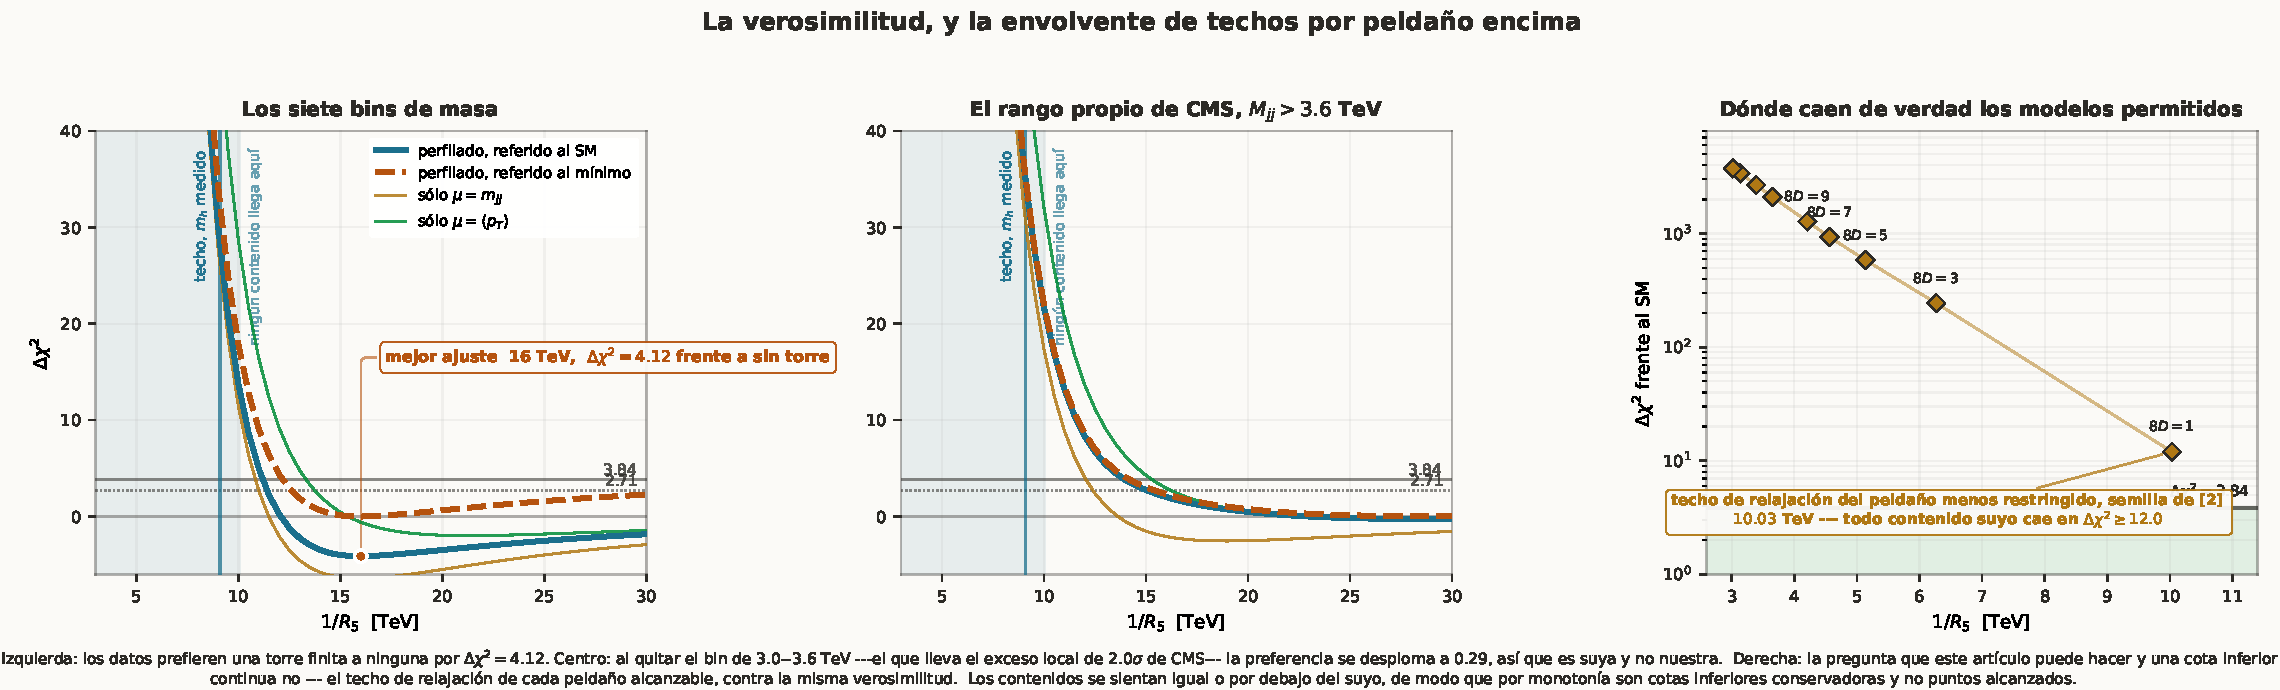
\includegraphics[width=\textwidth]{fig_chi2_es.pdf}
\caption{\textbf{La verosimilitud, y el peine de techos por peldaño puesto encima.} El $\chi^2$ del recast
de la \eqref{eq:chisq} frente a $1/R_5$, con las dos referencias dibujadas ---continua contra el
Modelo Estándar, que es la que usa la \eqref{eq:tulimit}, y discontinua contra el \emph{mínimo},
que es lo que el punto del $95\%$ de Wilks quiere decir de verdad---. Difieren porque el Modelo
Estándar no es el mejor ajuste. \emph{Izquierda, los siete bins de masa:} la curva toca fondo en un
$1/R_5=16$~TeV \textbf{finito}, $\Delta\chi^2=4.12$ por debajo de no tener torre ---$2.0\,\sigma$
nominales para un grado de libertad---. Las dos curvas finas son las dos elecciones de escala de
\cite{CMSangular} por separado, sin interpolar: acotan al resultado perfilado y tienen la misma
forma, de modo que el mínimo no es un artefacto del \emph{nuisance}. \emph{Centro, lo mismo sobre
$M_{jj}>3.6$~TeV}, que quita el bin de $3.0$--$3.6$~TeV: el mínimo se aplana y la preferencia se
desploma a $0.29$. \textbf{Así que la preferencia es el exceso local de $2.0\,\sigma$ de
\cite{CMSangular} en ese único bin, visto por nuestra plantilla, y no información que añada este
recast} ---por eso no se reclama significancia ninguna de él---. \emph{Derecha, la pregunta que una
cota inferior continua no puede hacer.} Los rombos son los techos por peldaño de la
\S\ref{sec:ceiling}, \eqref{eq:slope} ---el \emph{mayor} $1/R_5$ que el programa entero consiente
en cada $8D$ cuantizado---, leídos contra la misma verosimilitud, con $\Delta\chi^2$ en eje
logarítmico porque \emph{él} es el que abarca décadas: los dientes van sólo de $10.03$ a
$3.02$~TeV, mientras que su $\Delta\chi^2$ va de $12.0$ a varios miles. \textbf{Son techos de la relajación y no contenidos alcanzados}: el rombo de $8D=1$ está en
$10.03$~TeV mientras que el retículo sólo llega a $10.01$ ---los dos con la semilla que
\cite{KM25} imprimen--- y un contenido se sienta igual o por
debajo del techo de su peldaño, sobre el conjunto discreto que el peine aritmético permite.
\textbf{Eso no debilita la lectura: es lo que la convierte en una cota.} Como $\Delta\chi^2$
decrece monótonamente con $1/R_5$ en ese tramo ---medido, y cierto hasta $15.5$~TeV, muy por
encima del diente más alto---, un contenido igual o por debajo de su techo queda igual o
\emph{por encima} del $\Delta\chi^2$ de ese techo. De modo que cada rombo es una cota inferior
conservadora del $\Delta\chi^2$ de todo contenido de su peldaño, y el mínimo sobre los rombos
acota por debajo el mínimo sobre todos los contenidos sin necesidad de que ningún rombo sea
alcanzable. La banda por debajo
de $\Delta\chi^2=3.84$ está \textbf{vacía}: el diente más alto del peine es el techo de $8D=1$ en
$10.03$~TeV con la semilla que \cite{KM25} imprimen, y ni siquiera ése baja de $12.0$. \textbf{Ese panel está leído sobre el $\chi^2$ de
$77$ puntos}, el mismo del que se cita la \eqref{eq:tulimit}, y no sobre la curva de $70$ que
dibujan los otros dos ---por eso su punto de $8D=1$ no cae sobre la línea continua de su
izquierda---. Sobre aquella curva el mismo diente marcaría $13.4$; se cita el más débil de los dos.
Dibujada por
\texttt{make\_\allowbreak fig\_\allowbreak chi2.py} a partir de las corridas archivadas de
\texttt{scan\_\allowbreak mkk.py} y \texttt{ceiling\_\allowbreak ilp.py}.}\label{fig:chi2}
\end{figure}

\noindent\textbf{Y ese último panel es la pregunta que este artículo puede hacer y una cota
inferior continua no.} Un límite dice ``por encima de $10.86$~TeV''. Pero aquí $1/R_5$ no es
continuo: $8D$ es un entero impar con la semilla que imprime \cite{KM25}, de modo que los
techos por peldaño forman un \emph{peine} propio, y la
\eqref{eq:slope} da sus dientes ---$10.03$~TeV en $8D=1$, luego $6.27$, $5.14$, $4.56$, cayendo
hasta la asíntota de Lambert---. \textbf{Y no es el peine aritmético de la \S\ref{sec:pred}}:
aquél vive \emph{dentro} de un peldaño, con paso exacto en $M^2$, y es el conjunto de masas
que ese peldaño alcanza; éste tiene un solo diente por peldaño, y ese diente es lo más que el
peldaño alcanza, no todo lo que alcanza. Un contenido puede sentarse en cualquier punto igual
o por debajo del suyo. Leer el recast en cada diente, y no en una masa cualquiera, da
\begin{keyeq}
\begin{equation}\label{eq:combchi}
  \min_{k\ \mathrm{impar}}\ \Delta\chi^2\big(M_{\max}(k)\big)\;=\;12.0
  \qquad\text{en } 8D=1,\ 1/R_5=10.03\ \text{TeV,}
\end{equation}
\end{keyeq}
\noindent frente a un umbral de $3.84$; el diente siguiente está en $\Delta\chi^2=244$, y el
mejor de la rama del escape, $3.97$~TeV, por encima de mil ---los tres son $\Delta\chi^2$, no
masas. \textbf{Dos cosas de ese número son elecciones, y las
dos se hacen por el lado desfavorable.} Está leído sobre el $\chi^2$ de $77$ puntos ---el mismo
del que se cita la \eqref{eq:tulimit}, por ser el más débil--- y no sobre el de $70$, que daría
$13.4$; y los dientes son los techos por peldaño \emph{truncados}, $10.034$~TeV en $8D=1$, y no
el sin truncar $10.037$, que queda tres GeV más arriba y por tanto un pelo más abajo en
$\Delta\chi^2$. Ninguna de las dos vale un decimal por sí sola; se dicen las dos porque, si no, un
lector no puede saber cuál de los varios números disponibles se eligió.

\noindent\textbf{Y ahora la pregunta que importa más que las dos: ¿por qué carga con todo esto
\emph{un solo} diente?} Porque el techo por peldaño cae con $k$ ---$A_4$ no le puede seguir el
ritmo, y su tope por peldaño va $215,112,87,76,\dots$ por unidad de $8D$---, de modo que el diente
menos restringido es siempre el peldaño \emph{más pequeño}, y el más pequeño es $8D=1$ sólo porque
el Teorema~\ref{thm:eighths} dice que $8D$ es un \emph{entero} impar donde se cumple su hipótesis,
y con la semilla que imprime \cite{KM25} se cumple. \textbf{Así que el margen que
hay detrás de la \eqref{eq:combchi} no es $12.0$ frente a $3.84$: es la integralidad de $8D$}, y eso
se puede medir en vez de admirarlo: a $A_4$ fijo el techo va como $k^{-1/2}$, luego un cuanto la
mitad de grande pondría el diente más alto en $14.19$~TeV, donde este recast devuelve
$\Delta\chi^2=-6.0$ ---\emph{por debajo} del Modelo Estándar, dentro de la región que los datos
levemente prefieren---. Con el cuanto a la mitad la conclusión no se debilita: cambia de signo.

\noindent Merece seguir un paso más, porque acaba en un sitio concreto y el final no es una
debilidad. Con la semilla que imprime \cite{KM25}, $8D$ es impar porque la materia aporta una
cantidad par y el sector gauge una impar. Es
tentador atribuir esa imparidad a \emph{un solo medio} ---el peso $\tfrac12$ de cada par adjunto
con $P_6=-1$, frente al $2$ de cada par con $P_6=+1$---, pero no es eso lo que la carga, y la
distinción acaba decidiendo la cadena entera. Sobre los $n_+=2$ y $n_-=6$ pares de la fila que los
mezcla, el coeficiente vale $2n_++\tfrac12 n_-=4+3=7$: el término antiperiódico aporta $3$, un
\emph{entero}, y para que la suma salga impar hace falta además que el periódico sea par.
\textbf{Dos condiciones, no una, y ningún peso decide por su cuenta}
(Figura~\ref{fig:ghosts}). Ese medio no se lee de la ec.~(68)
de \cite{KM25} ---se \emph{infiere}, y por un ajuste que tenía por dónde fallar---. La Parte~VI
\cite{PartVI} construye los $48$ generadores del adjunto, le lee a cada uno su $(q,P_5P_5',P_6)$ y
ajusta \emph{dos} pesos a \emph{tres} coeficientes: las \emph{dos} filas sin ningún par con
$P_6=-1$ fijan el peso periódico cada una por su cuenta, y concuerdan; la fila restante fuerza
entonces que el antiperiódico valga exactamente $\tfrac12$, reproduciendo su $7$ como
$2\times2+6\times\tfrac12$, el reparto que su texto enuncia y nunca deriva. \textbf{Pero la
redundancia no está donde importa.} Tres coeficientes contra dos incógnitas está sobredeterminado
como \emph{sistema}, y es tentador contarlo como una prueba que pudo fallar. Pudo ---pero sólo del
peso periódico, que es el que restringen las dos filas de sobra---. El peso antiperiódico lo fija
una sola ecuación y no lo comprueba ninguna. Lo que concuerda no es lo que decide.

\noindent \textbf{Y entonces el medio no sobrevive, que es la parte que merece entenderse.} El peso
gauge ---escrito $\omega_g$, porque $W$ ya es el funcional de estabilidad de la
\S\ref{sec:ceiling} y la rama de Lambert, y tres objetos para una letra es uno de más--- es
$\omega_g=2n_++\tfrac12 n_-$ sobre los pares adjuntos con $P_6=\pm1$, y un censo de las $4096$
asignaciones diagonales admisibles devuelve, sin un solo contraejemplo, $n_-=2m$ ---donde $m$
cuenta los índices doblemente volteados respecto al par de la línea de Wilson---. Así que
$\omega_g=2n_++m$ \emph{es un entero}, y es impar exactamente cuando lo es $m$. En la asignación de
\cite{KM25}, $m=3$, y los tres índices que lo forman son los de color de sus ecs.~(78)--(79).
\emph{De modo que lo que hace impar a $8D$ no es un medio en absoluto: es la paridad de un conteo de
colores.} El $\tfrac12$ es la contabilidad que cuenta cada par una vez, y como los pares vienen de
dos en dos siempre reconstituye un entero. La cadena es entonces: $m=3$ es impar, luego $\omega_g$ es
impar, luego $8D$ es impar, luego $|D|\ge\tfrac18$, luego $1/R_5$ queda capado, luego la clase es
comprobable en un número finito de sitios ---y el techo que este artículo calcula es ese mismo
hecho leído por el otro extremo---.
\textbf{Todos los eslabones de esa cadena son sólidos; el primero es heredado.} Arranca en los
pesos $(2,\tfrac12)$ leídos de \cite{KM25}, y la \S\ref{sec:open} enseña qué le pasa a la cadena si
son $(\tfrac32,\tfrac12)$: no se rompe, baja un peldaño.

\noindent \textbf{Un eslabón de esa cadena está inferido y no derivado, y la diferencia es de
dirección.} Lo que la Parte~VI establece de forma independiente es la \emph{tabla}: sobre los $48$
generadores del adjunto, $(q,P_5P_5',P_6)$ es teoría de grupos y no se mueve, lo que descarta
cualquier error en las multiplicidades de \cite{KM25}. Lo que \emph{no} establece son los pesos
---y conviene ser exacto sobre cuál de los dos, porque ``tres coeficientes, dos incógnitas,
sobredeterminado'' no significa aquí lo que parece---. \textbf{Dos} de las tres filas no contienen
ningún par con $P_6=-1$, así que cada una fija el primer peso por sí sola, y su acuerdo \emph{es}
la redundancia. \textbf{Una} fila contiene los pares con $P_6=-1$, de modo que el segundo peso
queda fijado por una sola ecuación y sin nada contra lo que contrastarlo. \emph{Así que la
redundancia comprueba el peso periódico y sólo ése.}

\begin{figure}[t]\centering
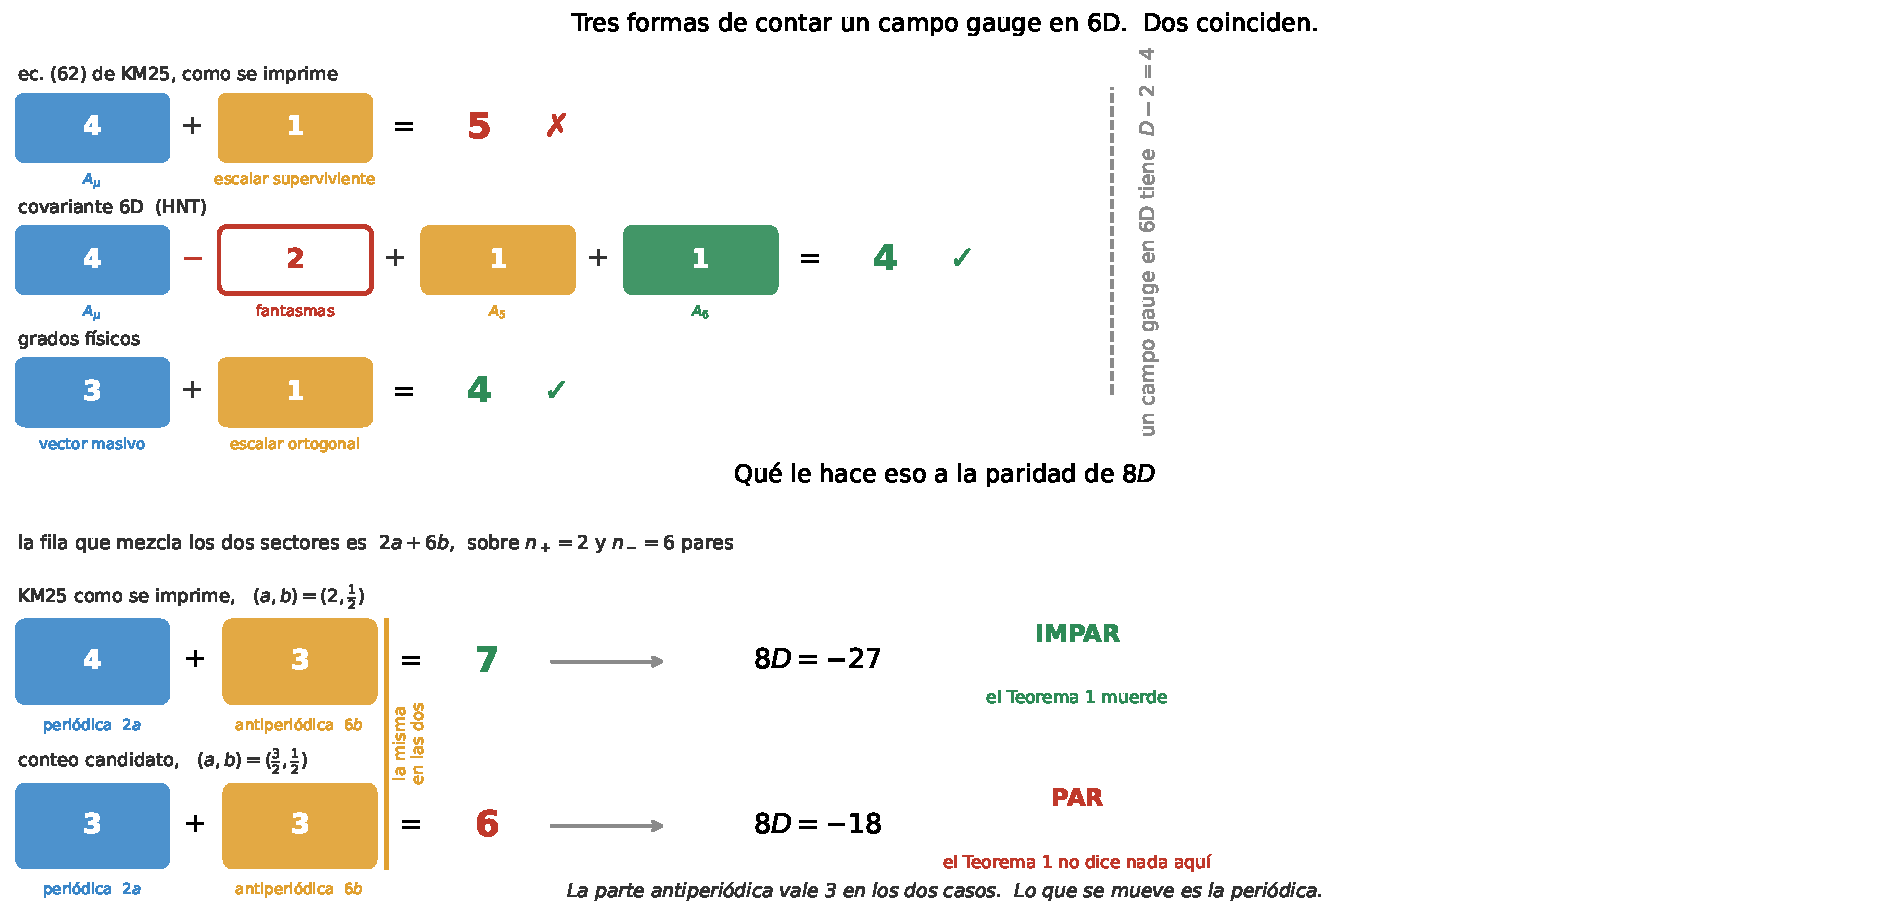
\includegraphics[width=\textwidth]{fig_ghosts_es.pdf}
\caption{\textbf{De dónde sale la paridad.} \emph{Arriba:} tres formas de contar los grados de libertad de un campo gauge en seis dimensiones. \cite{KM25} toman $4$ para $A_\mu$ y $1$ para el escalar superviviente; el conteo covariante en seis dimensiones de \cite{HNT} resta los dos fantasmas y se queda con las dos componentes extradimensionales, en consonancia con la regla general $-(D-2)$ de \cite{HY04}; el conteo físico usa las tres polarizaciones de un vector masivo. Dos de los tres dan $D-2=4$, y el que no es el que este artículo hereda. \emph{Abajo:} qué le hace eso a la fila que mezcla los dos sectores $P_6$, cuyo coeficiente es $2a+6b$ sobre $n_+=2$ y $n_-=6$ pares. La parte antiperiódica vale $6\times\tfrac12=3$ en los dos casos ---un \emph{entero}, y no se mueve---. Lo que se mueve es la periódica, de $4$ a $3$, y con ella la paridad: $7$ contra $6$, luego $8D=-27$ contra $-18$. De modo que el cambio de paridad no se le puede atribuir al semientero antiperiódico él solo ---el número que la \S\ref{sec:open} venía llamando el abierto---: lo que cambia es el carácter de paridad del coeficiente mixto completo, $2a+6b$. La figura se dibuja con el mismo mapa de cinco coordenadas que usa el texto, y se niega a dibujarse si no devuelve el $-27$ publicado.}\label{fig:ghosts}
\end{figure}

\noindent Y conviene decir cuál de los dos decide, porque una versión anterior de este párrafo lo
tenía al revés. La fila que los mezcla vale $2n_++\tfrac12 n_-$, y para que salga impar hacen falta
\textbf{dos} cosas a la vez: la parte periódica par \emph{y} la antiperiódica impar
(Figura~\ref{fig:ghosts}). La
antiperiódica es $6\times\tfrac12=3$, impar en cualquier caso, así que está a salvo. La periódica
es la que se mueve si el sector gauge lleva la resta de fantasmas, de $4$ a $3$. \emph{De modo que
la redundancia comprobó justamente el peso que decide, y lo comprobó en la única dirección que no
estaba en duda.} Y en los dos casos la inferencia va de sus números hacia los pesos, no de la geometría
hacia sus números. El orden causal es: contenido de campos en seis dimensiones $\to$ descomposición en modos
$\to$ pesos $\to$ coeficientes, y toda ruta de esta serie entra en esa cadena por el extremo
derecho. \textbf{Así que $(2,\tfrac12)$ es lo que los coeficientes exigen, no lo que la
compactificación predice}, y ningún cálculo de las Partes~I--VII lo deriva al revés. Qué lo haría:
una suma de Coleman--Weinberg sobre la torre de Kaluza--Klein hexadimensional con estas paridades de
orbifold, calculando el peso de un par con $P_6=-1$ desde su modeado antiperiódico en vez de
leerlo. Es un cálculo estándar y aquí no está hecho; la \S\ref{sec:open} lo recoge. Todo lo que
cuelga de los pesos está demostrado.

\noindent \textbf{Un intento de cerrarlo hacia adelante, y por qué falló ---que merece quedar
escrito porque el fallo enseña.} \cite{HY04} enuncian su regla de conteo con palabras: el potencial
es $[\text{d.o.f. fermiónicos}-\text{bosónicos}]$ por el potencial de \emph{un} grado de libertad,
que para gauge más fantasmas es $-(D-2)$; y su ec.~(3.10) da el del adjunto como peso $\tfrac12$
por par de carga, con un par en $c=2$ y dos en $c=1$ según su ec.~(3.8). Con $D=5$ eso devuelve su
propia ec.~(3.20), $(\tfrac32,3)$. Llevado a $D=6$ devuelve $(2,4)$, la parte periódica de la
ec.~(68) de \cite{KM25}, y por un momento lo tomamos por una derivación fuera de muestra.
\textbf{No lo es.} En seis dimensiones $D-2=4$ coincide numéricamente con el número de componentes
de $A_\mu$, que es cuatro en \emph{toda} dimensión; el acuerdo no distingue las dos contabilidades,
y en cinco ---donde difieren, $3$ contra $4$--- la que \cite{HY04} usan es $D-2$. Peor: $D-2$ es el
total sobre \emph{los dos} sectores de paridad, y asignárselo entero al periódico es justo el paso
que una segunda paridad prohíbe. De modo que el peso periódico sigue inferido y la salvedad de
arriba no se debilita.

\noindent \textbf{Y la misma aritmética, leída al revés, es una pregunta viva sobre la
contabilidad de \cite{KM25} que este artículo no puede zanjar y no debe esconder.} Su ec.~(62)
asigna $N=4$ a $A_\mu$ y, tras quitar la combinación de Goldstone, $N=1$ al escalar superviviente
de $A_{5,6}$. Con nuestra propia tabla de generadores ---un par en $c=2$, dos en
$(c{=}1,s{=}{+}1)$, y dos $P_6{=}{+}1$ más seis $P_6{=}{-}1$ en $(c{=}1,s{=}{-}1)$--- esos dos
números reproducen la ec.~(68) exacta: $2$, $4$ y $(2\times4+6\times1)/2=7$. \textbf{Pero $4+1=5$,
y un campo gauge en seis dimensiones tiene $D-2=4$ polarizaciones físicas.} \cite{HNT} hacen la
cuenta covariante en $T^2/\ZZ_2$ y lo dicen llanamente ---``the mass matrix for ghost fields is the
same as that for $A_\mu$''---, de modo que $A_\mu$ y fantasmas dan $4-2=2$ y las dos componentes
extradimensionales otros $2$: cuatro en total. Su orbifold no es éste ---\cite{KM25} usan el
producto $S^1/\ZZ_2\times S^1/\ZZ_2$, con dos reflexiones independientes---, así que lo que ellos
fijan es el total y no cómo lo divide una segunda paridad. Llevado al orbifold producto con
$R_5\gg R_6$, un recuento covariante resuelto por paridades \emph{sugiere} que los cuatro se
reparten $3$ del lado $P_6{=}{+}1$ y $1$ del otro, en vez de $4$ y $1$. Si eso fuera así,
sustituir $4\to3$ convertiría la ec.~(68) en $(\tfrac32,3,6)$, el $8D$ del sector gauge sería
$-18$ y no $-27$, \emph{par}, y \textbf{la hipótesis del Teorema~\ref{thm:eighths} no se
cumpliría} ---que es un enunciado distinto de que el teorema falle, y la diferencia es todo el
asunto. \textbf{No afirmamos que \cite{KM25} se
equivoquen}: en su contabilidad a un lazo no aparece ningún determinante de Faddeev--Popov, pero sí
un término de fijación de gauge, y podría haber una cancelación implícita en cómo construyen el
espectro. Lo que lo zanja es un cálculo que este artículo sólo hace en parte (\S\ref{sec:open}) ---el determinante en gauge de
fondo de \emph{una sola} órbita adjunta cargada, $\tfrac12\log\det\Delta_{A_\mu}
+\tfrac12\log\det\Delta_{A_5}+\tfrac12\log\det\Delta_{A_6}-\log\det\Delta_{\mathrm{FP}}$ con
$R_5/R_6\to\infty$, que no necesita $\su7$ ni cuarenta y ocho componentes. \emph{Mientras eso no
esté hecho, toda consecuencia de aquí que necesite el punto base gauge publicado hereda esta
pregunta ---que no es toda escala del lado teórico, porque la asíntota \eqref{eq:rinf} no lleva
cantidad gauge ninguna---, y es una pregunta más afilada que el
residuo del anclaje junto al que vive.}

\noindent \textbf{Y la exposición es más estrecha de lo que «un número inferido» hace pensar, cosa
que merece decirse porque corta hacia el otro lado.} La preocupación natural ---¿y si el peso no
fuera exactamente $\tfrac12$?--- es la pregunta mal puesta. Como $n_-=2m$ siempre, el peso gauge es
$\omega_g=2n_++2b\,m$. \textbf{Una versión anterior de este párrafo leía eso como un resultado de
robustez sobre $b$, y tenía el acento justo al revés.} En la fila que carga con la física, $n_+=2$
y $n_-=6$, la cuestión entera cabe en esto:
\begin{keyeq}
\begin{equation}\label{eq:twoparities}
  \begin{aligned}
    \omega_g\;&=\;2a+6b\;=\;(2a)+3\,(2b)\,,\\[2pt]
    \omega_g\ \text{impar}\;&\iff\;(2a)+(2b)\ \text{impar}\qquad(\text{si }2a,2b\in\ZZ)\,.
  \end{aligned}
\end{equation}
\end{keyeq}
\noindent Entran los dos pesos, en pie de igualdad, y ninguno decide solo:
\[
  (a,b)=\Bigl(2,\tfrac12\Bigr):\ 4+3=7\ \text{impar};\qquad
  (a,b)=\Bigl(\tfrac32,\tfrac12\Bigr):\ 3+3=6\ \text{par}.
\]
El peso antiperiódico es el \emph{mismo} en los dos y la paridad cambia igual. Así que la cadena no
cuelga de $b$, y $b$ nunca estuvo en peligro: lo que la \S\ref{sec:open} pone en duda es $a$, y la
\eqref{eq:twoparities} dice por qué eso basta. Medido en
\texttt{gauge\_\allowbreak weight\_\allowbreak origin.py} y
\texttt{gate\_\allowbreak km\_\allowbreak ghosts.py}. Lo que la \S\ref{sec:open} recoge es un hueco distinto y más estrecho: ninguna
comprobación \emph{publicada} pone a prueba ese peso. Todo anclaje contra el que se pueda
contrastar una curvatura se sitúa en $B=0$, donde el momento pesado por la paridad y el ciego a
ella coinciden; los resultados con reparto de paridad que \emph{sí} llevan sector antiperiódico
---el de \cite{CCD24} entre ellos--- viven en el peldaño del valor, $p=5$, y no llegan nunca a la
curvatura. Nuestra propia cadena
tiene dos patas; el mundo de fuera, ninguna. Quien tenga que decidir cuánto peso aguanta la
\eqref{eq:combchi} debe saber que es ahí donde vive ---y no en la estadística---. \textbf{Así que no es que la región permitida esté en parte
desfavorecida: ningún contenido del bulk que consiente la aritmética de la semilla que
\cite{KM25} imprimen llega a un $1/R_5$ en el que el $\Delta\chi^2$ de este recast baje de
$12.0$.} Todas las salvedades de los párrafos anteriores
siguen aplicándose a ese número, y ninguna de las variaciones \emph{cuantificadas} del lado del
colisionador se acerca al factor tres y
medio en $\Delta\chi^2$ ---pero es una cifra nominal de un $\chi^2$ gaussiano, no un $CL_s$, y así
se enuncia---. Lo que la hace digna de enunciarse es que son las dos mitades de este artículo
encontrándose: el programa entero dice qué escalas existen, y la verosimilitud dice qué opinan los
datos de ellas.
\paragraph{Y el canal que se había dejado fuera, puesto.} La \eqref{eq:tulimit} viste sólo $t$ y
$u$, y la razón para hacerlo es buena ---ahí el propagador resumado es real, luego no entran ni la
anchura ni $\mathrm{BR}(G_n\to jj)$, y el límite no depende de unas masas exóticas que el modelo
nunca fija---. \textbf{Pero ese argumento no demuestra que la omisión sea conservadora}, y no lo
es: las amplitudes interfieren, y en $q\bar q\to q\bar q$ el término temporal puede sumar a la
deformación de $t/u$ o restarle. Así que se calcula. Sólo dos elementos de matriz llevan gluón
temporal ---$q\bar q\to q\bar q$, por su pieza $s$ y por la interferencia $s$--$t$, y
$q\bar q\to q'\bar q'$, que es $s$ puro---; los estados finales con gluones quedan sin vestir por
el mismo argumento de cinco momentos de \cite{DMN01} usado arriba. El polo lo regula la anchura
\emph{total} $\Gamma_{\mathrm{tot}}=\Gamma_{q\bar q}+\Gamma_{\mathrm{exotic}}$ con
$\Gamma_{q\bar q}/M=2\alpha_s$ y $\Gamma_{\mathrm{exotic}}\ge0$ desconocida, de modo que
$\Gamma_{\mathrm{exotic}}$ se perfila en vez de elegirse.

\noindent Salen dos cosas, y la primera hace fácil la segunda. \emph{El desplazamiento encoge al
crecer la anchura} ---en $1/R_5=9.09$~TeV el cociente a QCD se mueve un $-0.47\%$ con
$\Gamma_{\mathrm{exotic}}=0$ y sólo un $-0.18\%$ con $\Gamma_{\mathrm{exotic}}/M=1$---, así que el
perfilado sobre $\Gamma_{\mathrm{exotic}}\ge0$ está acotado en la \emph{frontera}, y el peor caso
es una anchura que conocemos y no una que haya que barrer hasta el infinito. Y \emph{el signo es
negativo}, como la objeción sospechaba: quitar el canal $s$ no era conservador. Lo que vale es
poco. Ese $-0.47\%$ del cociente es un $-6\%$ de la \emph{deformación}, cociente menos uno, que es
lo que ve el ajuste; recalcular el límite en vez de reescalarlo ---la deformación no escala exacto,
los bins están correlacionados y la escala va perfilada--- da
\begin{equation}\label{eq:stu}
  \frac{1}{R_5}\Big|_{s+t+u,\ \Gamma_{\mathrm{exotic}}=0}=12.86\ \text{TeV}
  \qquad\text{frente a}\qquad
  \frac{1}{R_5}\Big|_{t/u}=12.99\ \text{TeV}\,,
\end{equation}
los dos a orden dominante y en la misma rejilla, de modo que el $-1.03\%$ entre ellos es el canal
$s$ y nada más. Eso apunta a un efecto de $\mathcal{O}(0.1~\text{TeV})$ sobre la
\eqref{eq:tulimit}, y las dos lecturas siguen por encima de $10.03$ en cualquier caso; el
desplazamiento exacto pide volver a correr el pipeline final de $77$ bins con $s+t+u$, y llevarse
un porcentaje a orden dominante de un cálculo a otro es justamente el reescalado que este artículo
se niega a hacer en todas partes. \textbf{Así que la omisión es real, su dirección es la desfavorable y su tamaño es un
uno por ciento} ---que merece decirse en ese orden---. Medido en
\texttt{s\_\allowbreak channel\_\allowbreak width.py}, cuyo primer control reconstruye el cálculo
entero desde cero y, con el canal $s$ apagado, reproduce la deformación $t/u$ archivada a
$6\times10^{-16}$; sin eso la diferencia no podría atribuirse al canal en vez de a la
reconstrucción.


\paragraph{Y lo que ese número no es.} \textbf{No} es una exclusión al $95\%$ de CL equivalente a
la de CMS, y la diferencia no es pedantería. \cite{CMSangular} pone límites con verosimilitudes
de Poisson a nivel detector, parámetros \emph{nuisance} perfilados y una construcción $CL_s$
asintótica; esto es un $\chi^2$ gaussiano sobre su covarianza publicada a nivel partícula con un
solo \emph{nuisance}. Los dos benchmarks del cierre miden ese hueco ---y lo miden \emph{distinto}, $1.03$
en el signo destructivo frente a $0.80$ en el constructivo, porque no son dos extracciones de una
misma incertidumbre. \textbf{Correr el mismo cierre sobre los límites \emph{esperados} dice cuál
de las dos explicaciones es.} Un conjunto Asimov ---la propia predicción del Modelo Estándar de
\cite{CMSangular} puesta en lugar de sus datos, en su mejor ajuste de escala y sin tocar la
covarianza--- devuelve $20.0$ y $29.0$~TeV frente a sus esperados publicados $18$ y $34$, es decir
$1.08$ y $0.85$. Son otra vez los cocientes observados, con cinco puntos de diferencia. \emph{Así
que el hueco es una propiedad del método y no de una fluctuación de este conjunto de datos
concreto}, cosa que un cierre sólo-observado nunca habría podido separar. Sitúa la
\emph{discrepancia de cierre dependiente del benchmark} en el nivel del diez al veinte por ciento
en $\Lambda$ sobre la selección de contacto emparejada, y mayor sobre las siete bandas
---que no es un sesgo estimado sobre un conjunto, porque no se ha construido ninguno: es el
desacuerdo medido sobre dos plantillas, su tamaño depende de sobre qué selección se mida, y no es
una banda trasladable a la
\eqref{eq:tulimit}---. Cambiar el signo de la interferencia cambia la forma, puede cancelarse
contra el término en $1/\Lambda^4$ y mueve qué bins dominan; leídos como coeficientes de
$1/\Lambda^2$ esos mismos dos cocientes pasan a ser $0.94$ y $1.56$, que es dependencia de
plantilla y no una calibración. \textbf{Así que son diagnósticos, y este artículo no los convierte en
una banda sobre la \eqref{eq:tulimit}.} Lo que sí puede decirse es que el recast encuentra
tensión suficiente para que cerrar la verosimilitud como es debido sea la prioridad, y que los
$3.97$~TeV quedan un factor tres por debajo de donde el recast pierde sensibilidad ---sin anchura
y sin $\mathrm{BR}(G_n\to jj)$ en ninguna parte, que es la razón entera de usar sólo los canales
espaciales. Lo que \emph{no} queda zanjado es el techo: $10.86$ y $13.75$ pasan los dos de $9.09$ y
de $10.03$, pero una sensibilidad nominal de recast no es el instrumento que puede retirar un
modelo, y la \S\ref{sec:open} dice qué lo sería. Medido
en \texttt{hadronic\_\allowbreak chi.py}, \texttt{cijet\_\allowbreak control.py},
\texttt{fetch\_\allowbreak hepdata.py}, \texttt{cms\_\allowbreak ci\_\allowbreak closure.py} y
\texttt{scan\_\allowbreak mkk.py}, con densidades partónicas de \cite{CT10} a través de
\cite{LHAPDF} y los coeficientes del operador de contacto de \cite{CIJET}.

\begin{keyeq}
De modo que los dos cálculos ya se cruzan \emph{numéricamente}: el techo algebraico de la
\S\ref{sec:ceiling} se acerca a $1/R_5$ por \emph{arriba}, en $9.09$~TeV, y la sensibilidad nominal
del colisionador por \emph{abajo}. Ascender la segunda a cota inferior experimental exige la
verosimilitud a nivel de detector, y la \S\ref{sec:open} lo dice; el cruce es lo que hace que valga
la pena hacerlo, no el resultado de haberlo hecho. \textbf{Y leído en el peine y no en una escala
continua, el cruce no es marginal}: la \eqref{eq:combchi} pone todo $1/R_5$ alcanzable en
$\Delta\chi^2\ge12.0$ ---con la semilla que \cite{KM25} imprimen, que es de quien es este
peine---. El diente más alto de la candidata es \emph{más bajo}, $7.38$~TeV, y el $\Delta\chi^2$
decrece monótonamente con $1/R_5$ en ese tramo (Figura~\ref{fig:chi2}), de modo que esa rama
queda más desfavorecida y no menos ---aunque no se ha leído diente a diente. Lo que sí es cierto ya sin nada de eso es la asimetría:
toda cota publicada sobre una escala de compactificación acota por abajo, y una cota inferior por sí
sola no puede excluir una clase ---la escala siempre puede subirse---. Es el techo lo que hace
finita la pregunta, y la cuantización lo que la hace afilada.
\end{keyeq}

\bridge{El diccionario está derivado, el único parámetro libre tiene nombre, la medida está
identificada y además hecha, y el peine se ha leído contra ella ---lo que deja sólo el instrumento
aritmético por contrastar contra la tabla de otros.}

% ===================================================================
\section{Un segundo anclaje}\label{sec:anchor}

La Parte~VI tiene un anclaje y falla. Con uno solo, un fallo no localiza nada: podría ser el
potencial, el desarrollo, el minimizador o el diccionario propio del modelo.

Von Gersdorff, Irges y Quir\'os \cite{vGIQ} aportan un segundo, independiente en grupo, dimensión,
década y autoría. Su modelo es pentadimensional en $S^1/\ZZ_2$ con una \emph{sola} paridad, de modo
que toda torre tiene modos enteros, no hay sector antiperiódico, $B_2=0$, y nuestro
$D=A_2-\tfrac34B_2$ colapsa a $D=A_2$: índice de Dynkin puro. \textbf{Su escenario es el rincón
$B=0$ de \eqref{eq:ladderab}}, y eso es lo que se pone a prueba, no lo que se supone. Merece
precisión de qué rincón se trata, porque $B=0$ no es $\Delta=0$: con una sola paridad
$\Delta_k=\mathcal{A}_k=S_k$, tan lejos de cero como el momento llega. Los dos sólo coinciden en el origen, y
la \S\ref{sec:open} gira precisamente sobre distinguirlos. Sus
convenios quedan fijados por sus propias notas al pie y no adivinados ---sus masas de bosones gauge
de Kaluza-Klein son ``$n^2$, $(n+2\omega)^2$, $(n-2\omega)^2$'', de modo que un estado de autovalor
de línea de Wilson $\lambda$ se desplaza en $q=2\lambda\omega$; y su nota al pie que identifica
$\alpha=2\omega$ convierte su fase en la nuestra.

\begin{center}\small
\rowcolors{2}{white}{okgreen!8}
\begin{tabular}{lll}
\toprule
\rowcolor{hdrblue!10}magnitud & suya & nuestra\\
\midrule
cargas del adjunto de $\su2$ & $n^2,(n\pm2\omega)^2$ & $c=-2,0,2$\\
$C_2(G)$, $C_R$ & de manual & $2,3$ y $1/2$, de generadores \emph{y} de Sage\\
su criterio, ec.~(5.3) & $C_G/C_R<4/3N_f$ & \emph{es} $D>0$\\
$N_f$ crítico, fundamental de $\su2$ & $3$ & $3$\\
$N_f$ crítico, fundamental de $\su3$ & $9/2$ & $9/2$\\
$N_f$ crítico, adjunto & $3/4$ & $3/4$\\
mínimo, adjunto de $\su2$ & $1/4$ & $1/4$, exacto\\
corchete de su ec.~(5.2) & $3C_2(G)-4C_RN_f$ & exacto, el $3\!:\!4$ incluido\\
\rowcolor{warmred!13}mínimo, adjunto de $\su3$ & $0.29$, $0.71$ & $1/3$ \emph{exacto}; abierto, abajo\\
\bottomrule
\end{tabular}
\end{center}

\noindent Los tres números críticos de sabores salen dos veces: de nuestro $D$, y de una segunda
derivada numérica de \emph{su} potencial, concordando a $10^{-6}$. Lo que sobra en el prefactor es
$2/\pi^2$ con ocho dígitos ---un número puro sin teoría de grupos ni zeta dentro, que son su $g^2$ y
su convenio de $A_5$ a $h$, con las $\pi$ que una reducción de Kaluza-Klein pone
ahí.

\paragraph{Un desacuerdo, y el control que lo dirime.} Para fermiones adjuntos publican dos mínimos
degenerados en $\omega\simeq0.29$ y $0.71$ en $\su3$. Nosotros obtenemos $\omega=1/3$
\emph{exactamente}, y por una razón: la estacionariedad es
$\mathrm{Sl}_4(\theta)+\mathrm{Sl}_4(2\theta)=0$, y en $\theta=2\pi/3$ la función de Clausen es impar
respecto de $2\pi$, luego $\mathrm{Sl}_4(4\pi/3)=-\mathrm{Sl}_4(2\pi/3)$ y la suma se anula
idénticamente. Con materia adjunta el potencial sólo ve el centro, de modo que el mínimo ha de ser
la holonomía simétrica bajo el centro ---el enunciado de manual de \cite{GPY}. El lazo de Polyakov
en la fundamental se anula en nuestro $1/3$ hasta $3\times10^{-31}$ y vale $0.168$ en $0.29$. La
evidencia está de nuestro lado; no podemos demostrar que su número de dos cifras sea un desliz, así
que queda registrado como abierto.

\begin{keyeq}
En cualquier caso el anclaje hace su trabajo. \textbf{El potencial, el desarrollo, $D$ y el
minimizador quedan validados, en el sector periódico $B=0$, contra un cálculo a un lazo publicado e
independiente}, de modo que el residuo $1.94/1.20$ de la Parte~VI frente a \cite{KM25} no puede
achacarse a lo que allí implementan. Lo que queda es el diccionario propio del modelo ---su
asignación de cargas y paridades, o la relación de $\alpha$ a $1/R_5$--- \emph{o} el sector
antiperiódico, que este anclaje no alcanza porque su modelo no tiene ninguno. En cualquier caso, un
sitio mucho más pequeño donde buscar.
\end{keyeq}

\noindent Alcance: esto ancla el rincón $B=0$. El sector antiperiódico, que es lo que hace de
este artículo lo que es, no queda anclado por él, porque su modelo no tiene ninguno.

\bridge{Qué se reclama, qué no, y qué se retiró por el camino.}

% ===================================================================
\section{Novedad, alcance, y qué no se reclama aquí}\label{sec:novel}

\paragraph{La contribución, dicha sin rodeos.} Del lado aritmético: la forma cerrada
\eqref{eq:amin} y su solución de Lambert-$W$ \eqref{eq:lambert} con las dos ramas y el pliegue, la
cancelación \eqref{eq:fpp}, las dos identidades sin logaritmo \eqref{eq:two}, los
Teoremas~\ref{thm:eighths} y \ref{thm:mod6} ---el segundo con \emph{cualquiera de las dos}
semillas gauge, el primero con su hipótesis dentro del enunciado---, la
ley geométrica de modos \eqref{eq:modes} y su forma cerrada
\eqref{eq:ladderab}--\eqref{eq:gaugerung}, la completitud de las cinco coordenadas \eqref{eq:UV},
el techo \eqref{eq:ceiling} con su certificado y su compañero sin truncar
\eqref{eq:rigorousceiling}, la cota del escape \eqref{eq:escapeceiling}, y el anclaje de la
\S\ref{sec:anchor}.

\noindent Del lado del colisionador, donde lo nuestro es menos y la raya importa más: la
\emph{lectura} de las tres matrices de paridad de \cite{KM25} que pone a todo bosón gauge que
cambia color en $1/R_6$ con función de onda nula en la brana de quarks, y la observación de que eso
contesta, para el canal gauge, la pregunta sobre desintegración del protón que ellos dejan abierta;
el recast \eqref{eq:chisq}--\eqref{eq:tulimit} de la distribución desplegada de \cite{CMSangular}
sobre el operador en octete de color de la torre, con sus pruebas de cierre; el coeficiente
\eqref{eq:codim2} de la sensibilidad logarítmica del segundo círculo; y la \eqref{eq:combchi}, que
lee esa verosimilitud en los dientes del peine de techos por peldaño y no en una masa
cualquiera, que es el
único sitio donde las dos mitades de este artículo se encuentran de verdad. \textbf{Lo que ahí
\emph{no} es nuestro}: la resumación \eqref{eq:resum} es la identidad de Euler y el propagador en
todos los canales es de \cite{DMN01}; las fórmulas de masa, acoplo y anchura del colorón son de
\cite{Simmons97}; la medida, su despliegue, su covarianza y su línea base del Modelo Estándar son
de \cite{CMSangular}; los coeficientes del operador de contacto son de \cite{CIJET}; y las
densidades partónicas son de \cite{CT10,NNPDF31,CT14} a través de \cite{LHAPDF}.

\paragraph{Relación con \cite{CCD24}, y dos afirmaciones retiradas.} La arquitectura del reparto
por paridad ---la suma partida según la condición de contorno, pesada por $\eta(p)/\zeta(p)$, con el
signo decidiendo la ruptura de simetría--- \textbf{está publicada}, en $p=5$ y al nivel del valor del
potencial. No la reclamamos. Tampoco reclamamos el \textbf{criterio de estabilidad del orbifold} de
la \S\ref{sec:ceiling}: que se evalúe el potencial en los dos puntos simétricos y se tome el menor,
que $F_-(0)=-\tfrac{15}{16}F_+(0)$ y $F_-(1/2)=F_+(0)$, y que las componentes $(\pm,\pm)$
estabilicen mientras las $(\pm,\mp)$ desestabilizan, son su \S2.2, sus ecs.~(2.12)--(2.13) y su
propia conclusión. La \eqref{eq:truevac} es eso sumado sobre un contenido de bulk y reescrito en la
notación de la \eqref{eq:F}; el contenido de la reescritura es que la suma resulta \emph{lineal} en
las multiplicidades, que es lo que le permite entrar en un programa entero ---y \cite{CCD24} no
calculan ninguna escala de compactificación, así que allí no aparece tal programa. Nuestro es esa
misma estructura de paridad en $p=3$, la curvatura, que su método no calcula y que es el peldaño que
necesita el vacío interior de $\alpha$ pequeño; su empaquetado como dos trazas de teoría de grupos
en lugar de recuentos de componentes; y toda consecuencia aritmética de las
\S\ref{sec:arith}--\S\ref{sec:ceiling}, los dos techos incluidos.

\paragraph{Relación con la literatura de términos cinéticos localizados en la brana.} La mitad de
bulk de la correspondencia también está publicada: \cite{CCP06} enuncia que el mismo factor de
índice de Dynkin que corre el acoplo gauge alimenta el término de masa del Higgs. Las trazas con
paridad insertada son estándar en la literatura de anomalías \cite{vGQ03,SS04}, que ---medido sobre
$94$ páginas--- no menciona nunca el potencial efectivo. Lo que no conseguimos encontrar enunciado en
ninguna parte es el puente: nadie escribe la curvatura como combinación de $T(R)$ y
$\mathrm{Tr}_R[P Q^2]$, y el peso $\eta(3)/\zeta(3)$ no aparece en este contexto.

El nulo se explica en lugar de limitarse a reportarlo. En $S^1/\ZZ_2$ un hipermultiplete no induce
\emph{ninguna} renormalización de los acoplos gauge de brana, y \cite{GNH05} muestra que no es una
cancelación supersimétrica ---las contribuciones bosónica y fermiónica se anulan por separado---, de
modo que en el caso que todo el mundo estudia no había nada que puentear; \cite{vGIQ} encuentran lo
mismo para las contribuciones de brana a la masa del Higgs. En seis dimensiones los acoplos de brana
sí renormalizan en orbifolds $\ZZ_N$ generales, pero \emph{no} en los puntos fijos $\ZZ_2$ de uno de
orden par \cite{GNH05}, y un \emph{fermión} de bulk no genera acoplo gauge localizado alguno: la
parte impar bajo paridad de su autoenergía lleva un tensor $\epsilon$ e integra a cero \cite{GLS06}.
\textbf{Por eso no identificamos $\mathrm{Tr}_R[P Q^2]$ con un acoplo gauge localizado en la brana.}
Ocupa la casilla $T^2$ de la familia de trazas con paridad insertada ---tadpole,
Fayet-Iliopoulos, término cinético gauge localizado, anomalía localizada---, pero para los fermiones
de bulk de este modelo esa casilla está vacía. Su papel aquí es el de la Parte~IV: el índice que
puede cancelarse, contrapuesto a la dimensión graduada que no puede.

\paragraph{Lo que las dos cuentas sí comparten, y es la función misma.} Por la fórmula de Hurwitz \cite{Hurwitz1882,Apostol},
$\zeta(1-s,a)=\Gamma(s)(2\pi)^{-s}\bigl[e^{-i\pi s/2}\mathrm{Li}_s(e^{2\pi i a})+\text{c.c.}\bigr]$,
el polilogaritmo de una fase de Wilson \emph{es} una zeta de Hurwitz con la fase en su segundo
argumento ---la casilla que allí ocupa el desplazamiento discreto del momento. Ghilencea, Lee y
Schmidt-Hoberg
\cite{GLS06} rastrean su divergencia de bulk hasta el polo simple de esa función en $z=1$, y nuestra
escalera alcanza el mismo polo: $\zeta[z,1]$ es la zeta de Riemann, y $p=5-2k$ termina en $p=1$. Qué
mitad lo alimenta lo fija entonces \eqref{eq:ladderab}: en $p=1$ el coeficiente antiperiódico
$2-2^{p}$ se anula, de modo que el polo lo alimenta el momento periódico $A_4$ y sólo él ---y
que el momento que sobrevive sea el que conserva el momento es sugerente de lo que ellos llaman
bulk; identificarlo con la estructura divergente localizada en el bulk, y el sector complementario
con los términos de borde, exige el cálculo explícito de contratérminos que pide la
\S\ref{sec:open}, y aquí no se afirma. Su regla de selección
es la nuestra en sus variables: los dos términos de Hurwitz entran como
$\zeta(z,1+c_1)+(-1)^{v}\zeta(z,1-c_1)$ y sobreviven sólo para $v$ par, que es la reflexión
$n\to-n$ por la que las cargas entran en nuestras tablas en pares $\pm Q$. Lo que difiere es la
función de Green, y por tanto la consecuencia: la suya es una divergencia ultravioleta de la
autoenergía del bosón gauge y necesita un contratérmino, mientras que la nuestra es un punto de
ramificación de un potencial \emph{finito} ---y el $H_4=\tfrac{25}{12}$ que lo resuelve es el que ya
lleva $G$ en \eqref{eq:moments}. Misma función, mismo polo, misma selección por paridad, y en
nuestra escalera lo alimenta sólo la mitad \emph{periódica}. Distinto correlador, distinta cura
---y si esa mitad periódica es el mismo objeto bulk que la suya es justo la pregunta de
contratérminos de arriba, que es por lo que la frase se para aquí---. Misma
mitad; distinto correlador, distinta cura.

\paragraph{Alcance de los resultados.} Un lazo. Espacio plano, no alabeado. Una torre de
Kaluza-Klein libre: sin masas de bulk y sin masas localizadas en la brana, cualquiera de las cuales
destruye el punto de ramificación. Una sola fase de Wilson ---con varias, la estacionariedad es un
sistema, y ése es el caso de dos fases de la Parte~V; para \emph{este} modelo no es restricción
ninguna, y el párrafo siguiente dice por qué. $\alpha$ pequeño: el desarrollo converge para
$|\alpha|<1/c_{\max}=1/3$ ---véase la \S\ref{sec:closed}: es un radio, no una salvedad
asintótica--- y truncarlo cuesta el $0.13\%$ cerca de $\alpha\approx0.02$ y un pequeño porcentaje
hacia $\alpha\approx0.25$. Y todo
escala del lado teórico arrastra el residuo del anclaje de la \S\ref{sec:setting}.

\paragraph{El espacio de moduli es el doblete de Higgs y nada más, y está medido.} Un lector que
cuente modos cero preguntará si el punto simétrico es un mínimo a lo largo de \emph{todas} las
direcciones planas o sólo de la que se minimiza. La pregunta tampoco es nuestra: \cite{HY04} abren
con ella ---el potencial a nivel árbol no puede fijar el vacío porque las fases de línea de Wilson
son planas, de modo que quien decide es el potencial a un lazo, y de él \emph{«podemos saber si el
color se conserva o no»}. En un modelo de gran unificación gauge-Higgs ésa es su forma afilada: si
alguna dirección plana lleva color, porque un moduli de línea de Wilson
coloreado es un leptoquark escalar con masa suprimida por lazo, y si bajara el potencial el vacío
rompería el color y todo número de aquí estaría calculado en un punto que no es el vacío. Las
direcciones planas son los modos cero de $A_5$ y $A_6$, y \texttt{moduli\_\allowbreak space.py} los
enumera desde sus ecs.~(3)--(10): catorce en $A_\mu$, que es el grupo no roto
$\su3\times\su2_L\times\mathrm{U}(1)^3$; cuatro en $A_5$, un solo doblete de $\su2_L$ sin color, que
es el Higgs; y \emph{ninguno} en $A_6$. El nulo no es un accidente del conteo sino de su convenio de
signos: su ec.~(4) da a $A_6$ el signo opuesto a $A_{\mu,5}$ bajo las reflexiones de $x_6$, así que
un modo cero de $A_6$ ha de ser impar bajo $P_6$, mientras que las ecs.~(7) y (9) lo quieren par
bajo $P_5$ y $P_5'$ ---y el bloque impar bajo $P_6$ es el rectángulo $3\times4$ fuera de la
diagonal, sobre el cual esas dos condiciones eligen columnas disjuntas. Cuatro moduli reales cuya
órbita genérica bajo $\su2_L\times\mathrm{U}(1)_Y$ es de dimensión tres dejan una sola fase, de modo
que minimizar en $\alpha$ minimiza sobre todo el espacio. El mismo guion reproduce su ec.~(57)
estado por estado, los $48$ generadores, que es lo que hace que un nulo merezca citarse.

Una precondición es heredada y no elegida, y pertenece a esta lista porque no está en nuestra mano
relajarla. El potencial de \cite{KM25} es sólo fermiones de bulk y gauge: descartan de plano la
contribución de los fermiones del Modelo Estándar, con el argumento explícito de que un quark
localizado en un punto fijo da $m_q(\alpha)^4\ln m_q(\alpha)^2\propto\alpha^4$ sin nada del factor de
realce que llevan los fermiones de bulk sin masa ---\emph{``a partir de esta observación, no
consideramos en este artículo el potencial procedente de las contribuciones de los fermiones del
ME''}. En $\amin\simeq0.05$ eso es $\alpha^4\sim 6\times10^{-6}$, y la omisión es segura a un lazo y,
con un $\alpha^2\sim0.25\%$ de la curvatura, sigue estando un orden por debajo del margen a dos
lazos de la Parte~VI \cite{PartVI}. Queda registrada porque todo número de aquí está calculado sobre
\emph{su} potencial, y un lector con derecho a preguntar qué hay dentro no debería tener que
reconstruir la respuesta a partir de su §5.

\paragraph{Y $g_4$ no hace falta elegirlo.} Toda escala del lado teórico de aquí pasa por el
$K=(\sqrt3/2\pi^3)m_Wg_4$ de la \S\ref{sec:mh}, luego $\mu\propto g_4^{-2}$ y el techo de la
\S\ref{sec:ceiling} depende de él. El valor usado en todo el texto es $g_4=0.63$, el acoplo
$\su2_L$ del Modelo Estándar corrido hasta la escala de compactificación, mientras que el anclaje
hermano lo toma a la escala débil: \cite{AHMN} escriben $g_4=2m_W/v\simeq0.653$ bajo su ec.~(4.4).
Versiones anteriores de este artículo dejaban los dos uno al lado del otro como una elección
declarada. Son el mismo acoplo en dos escalas ---$g_2(M_Z)=0.6517$ y $g_2=0.630$ en $5.6$~TeV--- y
la elección se puede quitar, porque la escala a la que hay que evaluar $g_4$ es la propia respuesta.
Imponiendo
\begin{equation}\label{eq:g4fix}
  g_4\;=\;g_2\!\left(1/R_5\right),\qquad 1/R_5=\frac{2\pi m_W}{x},\qquad
  x^2=\frac{12\zeta(3)D}{A_4+6\mu},\qquad \mu=\Bigl(\frac{m_h}{K\pi^2}\Bigr)^{2}
\end{equation}
se cierra el lazo de autoconsistencia ---llamado así, y no cierre, porque la
\S\ref{sec:collider} ya gasta esa palabra en los benchmarks del recast---. La aplicación contrae
con fuerza ---su derivada en el punto fijo es
$6.5\times10^{-3}$, y todo arranque entre $0.30$ y $1.30$ converge al mismo sitio en siete pasos---
y da
\begin{equation}\label{eq:g4star}
  g_4^\star=0.6275 ,
\end{equation}
a un $0.39\%$ del valor aquí usado, dejando el vértice en $A_4=104$ y $1/R_5$ en $9248$ en vez de
$9218$~GeV.

\noindent \textbf{Pero eso no quita la elección ---y conviene decir tanto por qué no como hasta
dónde llega el decirlo.} La
\eqref{eq:g4fix} fija $g_4$ \emph{dado} que se evalúa en $1/R_5$, y una escala de emparejamiento
es un convenio como cualquier otro. Bajarla un factor dos, hasta $1/2R_5$, lleva $g_4^\star$ de
$0.6275$ a $0.6310$: una dispersión del $0.56\%$, y no mueve el vértice. \textbf{Y eso es todo lo
que un running cuatridimensional tiene derecho a decir aquí}, porque $1/R_5$ es donde arranca la
torre de Kaluza-Klein ---la \S\ref{sec:open} usa ese mismo hecho en la otra dirección, que por
debajo de $1/R_5$ la teoría es el Modelo Estándar. Por encima, el running del Modelo Estándar
ya no vale por sí solo, porque entran los umbrales de Kaluza-Klein; lo que lo sustituye es un
cálculo que este artículo no hace---. Estirar la escala de emparejamiento hasta $2\pi/R_5$, seis
niveles más arriba, daría $0.6186$ y llevaría el vértice a $A_4=107$; ese número queda archivado
como marca de lo que \emph{no} está zanjado y a propósito no se cita aquí como sistemático.
\textbf{Así que $g_4$ sigue siendo un dato ---la escala de emparejamiento es un convenio, esto no
lo quita, y el tamaño de esa libertad no queda establecido aquí.} Establecerlo pide el
emparejamiento de la propia torre con el acoplo $\su7$ del bulk, que es la segunda condición que
el mismo guion registra y que este artículo no intenta. El artículo mantiene $0.63$, y la frase que siempre ha llevado ---los dos valores
defendibles, la elección no libre--- queda tal cual. Lo que el lazo de autoconsistencia sí
establece es más pequeño y aun así vale: dada una escala de
emparejamiento, el valor es un punto fijo que contrae con fuerza y no un ajuste, y los dos números
de la literatura son un mismo acoplo en dos escalas, $g_2(M_Z)=0.6517$ y $g_2=0.630$ en $5.6$~TeV.
Con el valor a la escala débil, $0.653$, el vértice se mueve al otro lado, a $A_4=98$ y $8903$~GeV.
Medido en \texttt{running\_\allowbreak g4.py}, con el correr en cuatro dimensiones importado de
\texttt{running\_\allowbreak gap.py} en vez de reescrito.

\paragraph{Lo que probamos y retiramos.} Tres lecturas murieron mientras se hacía este artículo, y
quedan registradas porque sus muertes son informativas. Una casi cancelación cuantizada entre las
piezas de bulk y de brana se midió antes de escribirla y resultó ser un efecto del $10\%$, no del
$90\%$ ---lo que sobrevive es que las cinco filas publicadas caen entre el percentil cuarto y el
noveno de ese cociente, de modo que la cancelación es lo que la viabilidad fenomenológica
\emph{selecciona}, no un mecanismo. Una lectura en la que el corchete de la tabla gauge era igual al
número de colores, que habría hecho del Teorema~\ref{thm:eighths} y de la muerte de la obstrucción en
$k=2$ dos factores de un mismo producto, vale en su asignación de paridades y falla en $3872$ de las
$4096$ admisibles. Allí el instinto era bueno y el objeto era el equivocado: los dos hechos \emph{son}
uno, y lo que los une es el coeficiente $2-2^{p}$ de \eqref{eq:ladderab} ---par en $p=5,3$, que es la
protección por paridad, y cero en $p=1$, que retira la contribución \emph{antiperiódica} ---con la
semilla que \cite{KM25} imprimen ésa es la muerte de la obstrucción, mientras que con la candidata
deja un sector periódico impar llevándola---. Y una identificación de una dirección
ciega del potencial resultó ser supersimetría, que la propia fuente discute.

\bridge{Lo que deja abierta la pregunta que toda cota debe: qué tendría que ser cierto para que los
números absolutos signifiquen lo que parecen significar ---y qué, en este artículo, los sostiene
todavía en vez de estar sostenido por ellos.}

% ===================================================================
\section{Lo que esto deja abierto}\label{sec:open}

\begin{itemize}\itemsep2pt
\item \textbf{El anclaje.} La \S\ref{sec:anchor} lo estrecha hasta el diccionario propio del modelo,
pero no lo cierra. La prueba más afilada que queda es una segunda tabla publicada para un modelo que
cumpla las cinco precondiciones; un cribado de la literatura encontró exactamente uno, el estudiado, y
la razón es estructural y no accidental.
\item \textbf{Averiguar cómo se reparten los cuatro grados de libertad del sector gauge entre los
dos sectores $P_6$.} Es lo más agudo que queda abierto. Y no es el problema que nombraba una
versión anterior de esta lista, así que conviene decir la corrección con todas las letras.

\emph{El total está zanjado.} Coinciden tres artículos publicados. \cite{HY04} dan el factor
gauge-más-fantasma como $-(D-2)$, llaman a los coeficientes ``numbers of d.o.f.'' y dicen que su
método ``is available for more than $5$ dimensional gauge theories''. \cite{HNT} hacen la cuenta en
\emph{seis} dimensiones y sobre un orbifold $T^2/\ZZ_2$, y enseñan los pasos: los fantasmas tienen la
misma matriz de masas que $A_\mu$, así que ``contributions to the effective potential from $A_\mu$
and ghosts are, therefore, $4-2=2$''. Los dos componentes extradimensionales aportan otros dos.
Cuatro en total. Y \cite{AHMN} toman $N=4$ para todo el sector gauge de un modelo
hexadimensional sobre $T^2/\ZZ_2$. Cuatro, tres veces.

\emph{Y la geometría es justamente la razón de que eso sea el total y no el reparto.} \cite{KM25}
compactifican sobre $S^1/\ZZ_2\times S^1/\ZZ_2$ ---cada coordenada extra en su propio círculo, con
\emph{dos} reflexiones independientes, que es de donde salen $P_5$ y $P_6$ y por qué este artículo
tiene dos sectores de paridad entre los que repartir cuatro grados de libertad---. \cite{HNT} y
\cite{AHMN} trabajan sobre $T^2/\ZZ_2$, con una sola $\ZZ_2$ actuando a la vez sobre las dos
coordenadas. De modo que zanjan cuántos grados de libertad hay, y no pueden zanjar cómo se los
repartiría una segunda paridad independiente. Eso no es un hueco de sus artículos: es la razón de
que la pregunta que este artículo tiene que hacerse siga abierta.

\emph{Aquí un poco de historia vale el espacio, porque explica cómo se pierde una cuenta que ya
estaba hecha.} La idea de que el Higgs sea una componente extradimensional de un campo gauge es de
1979 \cite{Manton}; el mecanismo que le da potencial es de 1983 \cite{Hosotani}. La contabilidad a
un lazo llegó mucho después y, da la casualidad, dos veces en la misma temporada: Haba y Yamashita
publicaron la fórmula general pentadimensional en enero de 2004 \cite{HY04}, y Hosotani, Noda y
Takenaga publicaron la cuenta hexadimensional sobre $T^2/\ZZ_2$ dos meses más tarde \cite{HNT}.
Uno da el coeficiente como $-(D-2)$ y lo deja ahí; el otro escribe la resta con todas las letras.
\textbf{El conteo total de grados de libertad quedó zanjado hace más de dos décadas. El reparto por
paridades que este modelo necesita, no}, y decirlo así hace nuestra aportación más nítida, no más
pequeña.

Ninguno de los dos está en la lista de referencias de \cite{KM25}. Takenaga sí, por un artículo de
2007; Hosotani también, por los de 1983 y 1989. Lo decimos como diagnóstico y no como queja ---las
listas de referencias son finitas, y la suya es larga---, pero es el mecanismo, y conviene verlo
sin adornos. Un resultado que un campo zanja en dos artículos de una misma primavera puede caerse
igualmente de la cadena de citas que hereda un modelo posterior, y una vez fuera de la cadena
puede volver a derivarse de otro modo, de buena fe, décadas después. \emph{Tampoco nosotros
habríamos mirado, si un número hubiera salido bien.}

\emph{Lo abierto es el reparto, y lo útil es que enseñen los pasos.} La \S\ref{sec:collider}
objeta que $D-2=4$ coincide en seis dimensiones con el número de componentes de $A_\mu$, de modo
que un total pelado no distingue las dos contabilidades. Es cierto ---pero \cite{HNT} no escriben
$4$; escriben $(4-2)+2$, y eso sí las distingue. Lo que llevan es una paridad, no dos, así que
fijan el total y no dicen nada de cómo se divide, y la segunda paridad es justo sobre lo que gira
este modelo. Leídos
como pesos por par cargado, los coeficientes de \cite{KM25} son $(2,\tfrac12)$: cuatro grados de
libertad en el canal periódico y uno en el antiperiódico. Eso son cinco. Un conteo covariante que
conserve las dos paridades \emph{sugiere} $(\tfrac32,\tfrac12)$: tres y uno, que son cuatro.
\textbf{Escribimos «sugiere» y lo decimos en serio.} Ese candidato correspondería a que la resta de
fantasmas que falta viva en el sector periódico; lo que lo establecería es el operador cuadrático,
las condiciones de contorno de $A_\mu$, $A_5$, $A_6$ y el par de fantasmas, y el determinante que
den ---y ése es justamente el cálculo que este punto existe para pedir---. No puede ser a la vez un
resultado y un cálculo que nadie ha hecho. Lo que sí podemos decir sin él es más estrecho y sigue
siendo útil: ningún cambio de normalización produce la diferencia, porque un factor común movería
los tres coeficientes a la vez y éstos se mueven por $\tfrac43$, $\tfrac43$ y $\tfrac76$.

\emph{Y el peso que decide es el periódico.} Una versión anterior de esta lista decía lo contrario.
La fila que los mezcla recorre $n_+=2$ pares periódicos y $n_-=6$ antiperiódicos, luego su
coeficiente es $2n_++\tfrac12 n_-$. Para que salga impar hacen falta dos cosas a la vez: la parte
periódica par y la antiperiódica impar. La antiperiódica es $6\times\tfrac12=3$, impar en
cualquier caso. La periódica es la que mueve la resta de fantasmas, de $4$ a $3$. Así que la
sobredeterminación del ajuste comprobó el peso periódico ---que resultó ser el que importa, y el
que ahora está en duda--- (\texttt{gauge\_\allowbreak weight\_\allowbreak origin.py},
\texttt{gate\_\allowbreak km\_\allowbreak ghosts.py}).

\emph{Cerrar esto pide un cálculo, no otra comprobación}: un determinante en gauge de fondo para
una sola órbita cargada, conservando las dos paridades, que devuelva el reparto y no sólo el total.
Mientras eso no exista, todo lo que aquí necesita que el desplazamiento gauge sea \emph{impar}
queda condicionado a la ec.~(68) de \cite{KM25} tal como está publicada.

\emph{Y parte de ese cálculo ya está hecha, lo cual cambia lo que queda abierto sin cerrarlo.} Con
la línea de Wilson plana, $F_{MN}=0$, el operador cuadrático en un modo de momento $p_M$ es
$\Delta_{MN}=p^2g_{MN}-(1-\xi^{-1})p_Mp_N$: una actualización de rango uno de $p^2$, con un
autovalor longitudinal $p^2/\xi$ y $D-1$ transversos $p^2$. El término en $\xi$ \emph{sí} mezcla
los dos sectores de paridad en general, porque $\Delta_{6a}\propto p_6$ ---de modo que la pregunta
era legítima y no una formalidad---. Pero la dependencia en $\alpha$ del $\mathrm{Li}_5$ dominante
que retiene la \S\ref{sec:setting} vive en $p_6=0$ ---los modos con $p_6\neq0$ también dependen de
$\alpha$ en la teoría hexadimensional completa, y sencillamente están suprimidos en el límite que
este artículo adopta en todas partes---, donde ese
factor se anula, y donde de todas formas sólo hay presente una clase de paridad: para un generador
$P_6=\varepsilon$, $A_\mu$ y $A_5$ llevan cosenos y tienen modo cero mientras que $A_6$ lleva senos
y no lo tiene. Lo que queda, sector a sector, es
\begin{equation}\label{eq:xisplit}
  \varepsilon=+1:\ \ \tfrac12\bigl[5\ln p^2-\ln\xi\bigr]-\ln p^2=\tfrac32\ln p^2-\tfrac12\ln\xi,
  \qquad
  \varepsilon=-1:\ \ \tfrac12\ln p^2,
\end{equation}
o sea $3$ y $1$, que suman el $D-2=4$ de \cite{HY04}. El $\ln\xi$ que sobrevive no lleva $p$, y eso
por sí solo no basta para descartarlo ---sumada sobre una torre \emph{desplazada}, una constante
sin $p$ no tiene por qué ser independiente de $\alpha$, porque $\zeta_H(0,a)=\tfrac12-a$ se mueve
con el desplazamiento---. Se descarta porque las dos mitades de la torre se cancelan,
$\zeta_H(0,a)+\zeta_H(0,1-a)=0$ para todo $a$, y además porque la integral cuadridimensional de un
coeficiente sin $p$ no tiene escala. \textbf{De modo que el reparto no depende de $\xi$, y vale
$(a,b)=(\tfrac32,\tfrac12)$: la semilla candidata.} Medido en
\texttt{gauge\_\allowbreak xi\_\allowbreak independence.py}, cuyo señuelo ---fantasmas con la
paridad de $A_6$ en vez de la de $A_\mu$--- devuelve $5$ y $1$ y no pasa la prueba de $D-2$, de
modo que la hipótesis está haciendo trabajo.

\emph{Lo que eso no zanja son dos cosas y media, y conviene separarlas.} Que los fantasmas hereden
la paridad de $A_\mu$ se \emph{toma}, con el argumento estándar de que el parámetro gauge no lleva
índice vectorial; es lo que hacen \cite{HNT}, y el señuelo enseña que la respuesta depende de
ello ---pero suponerlo no es demostrarlo---. Si la construcción del espectro de \cite{KM25}
esconde una cancelación que reponga el grado que falta es una pregunta que sólo pueden contestar
sus autores. Y la media: todo esto es a orden dominante en $R_5/R_6$, que \cite{KM25} piden grande
sin fijarlo, de modo que a cociente moderado habría que rehacer la cuenta.
\textbf{El Teorema~\ref{thm:eighths} sigue por tanto condicionado, y el aviso de portada sigue con
él.} Lo que ha cambiado es que la bifurcación ya no es simétrica: la maquinaria de este mismo
artículo apunta ya a la rama en la que la hipótesis de ese teorema \emph{no} se cumple.
\textbf{Pero apunta una vez, no dos.} La \eqref{eq:xisplit} y la prueba de la resta de fantasmas de
\texttt{single\_\allowbreak orbit\_\allowbreak determinant.py} comparten la asignación que decide
la respuesta ---que los fantasmas lleven la paridad de $A_\mu$---, de modo que son dos
implementaciones de un supuesto y no dos comprobaciones independientes. Una versión anterior de
este párrafo las llamaba caminos distintos; no lo son, y la distinción es toda la razón por la que
el supuesto merece derivarse en vez de enunciarse.

\emph{Y se deriva, en tres líneas, de la invariancia gauge.} Bajo la reflexión de $x_6$ un generador
cumple $P_6T^aP_6^{-1}=\eta_aT^a$. La variación gauge $\delta A_M=D_M\omega$ fija entonces la
paridad del parámetro, y no al revés: $\delta A_\mu=\partial_\mu\omega+i[A_\mu,\omega]$ no lleva
derivada en $x_6$, luego $\omega^a$ ha de compartir la paridad $\eta_a$ de $A_\mu^a$; y
$\delta A_6=\partial_6\omega+i[A_6,\omega]$ sale entonces impar donde $A_6$ lo es, porque
$\partial_6$ cambia el signo. El funcional de fijación de gauge de fondo $\bar D_M\delta A^M$ tiene
paridad $\eta_a$ por lo mismo, de modo que respeta las condiciones de contorno en vez de imponer
otras. BRST sustituye $\omega^a$ por $c^a$ en $sA_M=D_Mc$, luego $c^a$ y $\bar c^a$ llevan también
$\eta_a$. \textbf{Los fantasmas heredan por tanto la paridad de $A_\mu$ como consecuencia de la
acción del orbifold sobre el parámetro gauge, y no por convenio}, que es lo que la
\eqref{eq:xisplit} necesitaba y aquello de lo que el señuelo de
\texttt{gauge\_\allowbreak xi\_\allowbreak independence.py} enseña que depende la respuesta.

Lo que eso deja abierto es más estrecho que antes, y conviene nombrarlo exacto. Si la construcción
del espectro de \cite{KM25} esconde una cancelación que reponga el grado que falta es una pregunta
que sólo pueden contestar sus autores. Y el reparto de arriba se deriva en la teoría reducida
$R_5/R_6\to\infty$ ---el mismo límite en el que la \S\ref{sec:setting} adopta el potencial de
$\mathrm{Li}_5$, de modo que es el alcance en el que ya trabaja todo el artículo y no una
debilidad propia de este cálculo---. \textbf{El Teorema~\ref{thm:eighths} sigue condicionado y el
aviso de portada sigue con él}, porque una derivación nuestra no es un enunciado sobre lo que
\cite{KM25} hicieron. Preferimos escribirlo a dejar que una cota siga apoyada en la rama que le
conviene.

\emph{Y tampoco explica la otra cuestión abierta, que merece medirse en vez de suponerse.} El
residuo del anclaje de la \S\ref{sec:setting} y la semilla gauge son los dos sobre los
coeficientes de \cite{KM25}, de modo que un lector tiene derecho a preguntar si son un solo
problema. No lo son. Minimizar el potencial exacto de las cinco filas publicadas con la semilla
candidata lleva $\amin^{\text{nuestro}}/\amin^{\text{suyo}}$ de $1.03$--$2.08$ a $1.24$--$3.20$
---peor en las cinco filas sin excepción, y el $|\text{razón}-1|$ medio de $0.50$ a $1.13$---.
\textbf{De modo que ninguno de los dos hallazgos avala al otro}: la pregunta de los fantasmas se
sostiene o se cae por el determinante, y no por esa columna. Ni podría arbitrarla esa columna,
porque no la reproducimos con \emph{ninguna} de las dos semillas, y un instrumento que no
reproduce su referencia no puede ser testigo de nada. Medido en
\texttt{ghost\_\allowbreak seed\_\allowbreak vs\_\allowbreak anchor.py}, cuya falsación escala
el sector gauge por $0.2$ hasta $0.8$ y ve el residuo empeorar monótonamente ---de modo que
«empeora» es una medida que la prueba podía haber desmentido y no desmintió.

\emph{Pero sí podemos decir lo que cuesta la otra rama, y cuesta menos de lo que parece.} Correr el
mismo programa entero con la semilla candidata es un cambio pequeño: los momentos por multiplete
son \emph{diferencias} contra el sector gauge, así que no se mueven en absoluto; sólo se mueve el
punto base. De ahí salen tres cosas, y sólo una es una pérdida. La ley mod~$6$ sobrevive literal:
el subgrupo del retículo no cambia y sólo se desplaza su punto base, de modo que $8D\equiv 2A_4+3$
sigue valiendo, sin una sola violación en $20\,000$ contenidos aleatorios con cada semilla. El
Teorema~\ref{thm:eighths} era su \emph{corolario} bajo «$A_4$ entero», y es $A_4$ al volverse
semientero lo que cambia $2A_4+3$ de impar a par. El teorema de $2W$ sobrevive intacto, porque el
sector gauge aporta $2W=-3$, impar, con \emph{las dos} semillas. Y el techo también sobrevive, más
bajo: el menor peldaño positivo \emph{físicamente admisible} pasa de $D=\tfrac18$ a
$D=\tfrac28$ ---en la rama candidata el retículo alcanza $D=0$, como dice el párrafo siguiente, y
lo que lo retira allí es la identidad~(II) y no la aritmética; con la semilla que \cite{KM25}
imprimen $8D$ es impar y lo retira la aritmética--- y como el
techo por $D$ baja de forma monótona, la cota baja con él, de $10.03$ a $7.38$~TeV
(Figura~\ref{fig:coset3d}). \textbf{Esos dos números son el mismo tipo de objeto y sólo ése}: los
dos son la cota dual certificada sobre el cono de momentos, de modo que $7.38$ es el análogo del
$10.03$ en la rama candidata y de nada más. La rama publicada tiene dos niveles más por debajo
---$10.01$~TeV \emph{alcanzado} al levantar el retículo, y $9.22$~TeV al exigir que el vacío sea el
verdadero---. \emph{Ninguno de los dos se ha recalculado en la rama candidata}, y mientras no se
haga, comparar $7.38$ con $9.22$ sería comparar una cota con un óptimo.

\emph{Y esa tabla tiene una consecuencia estructural que merece decirse, porque va en dirección
contraria a lo que suele costar una bifurcación.} Los $7.38$~TeV de la rama candidata son una cota
alcanzada \emph{sin} imponer la condición de vacío verdadero, e imponerla sólo quita contenidos
del conjunto factible, de modo que el techo de vacío verdadero de esa rama sólo puede ser todavía
menor. \textbf{Entre las dos semillas que este artículo considera, y sobre la superficie
algebraica de tres peldaños, los $9.22$~TeV siguen siendo por tanto la cota conservadora.} La
ambigüedad de la semilla gauge no abre una vía hacia escalas de compactificación mayores: cierra
una. Lo que mueve es la explicación y el filo ---en qué peldaño se sienta el máximo, y si lo que
prohíbe $D=0$ es un teorema o una identidad---, y no el número que se le pide al lector no
rebasar. Las dos salvedades cargan peso y ninguna es adorno: aquí no se costea una tercera
semilla, y fuera de la superficie de tres peldaños la cuestión sin truncar de la
\S\ref{sec:ceiling} sigue abierta con las dos ramas.

\begin{figure}[t]\centering
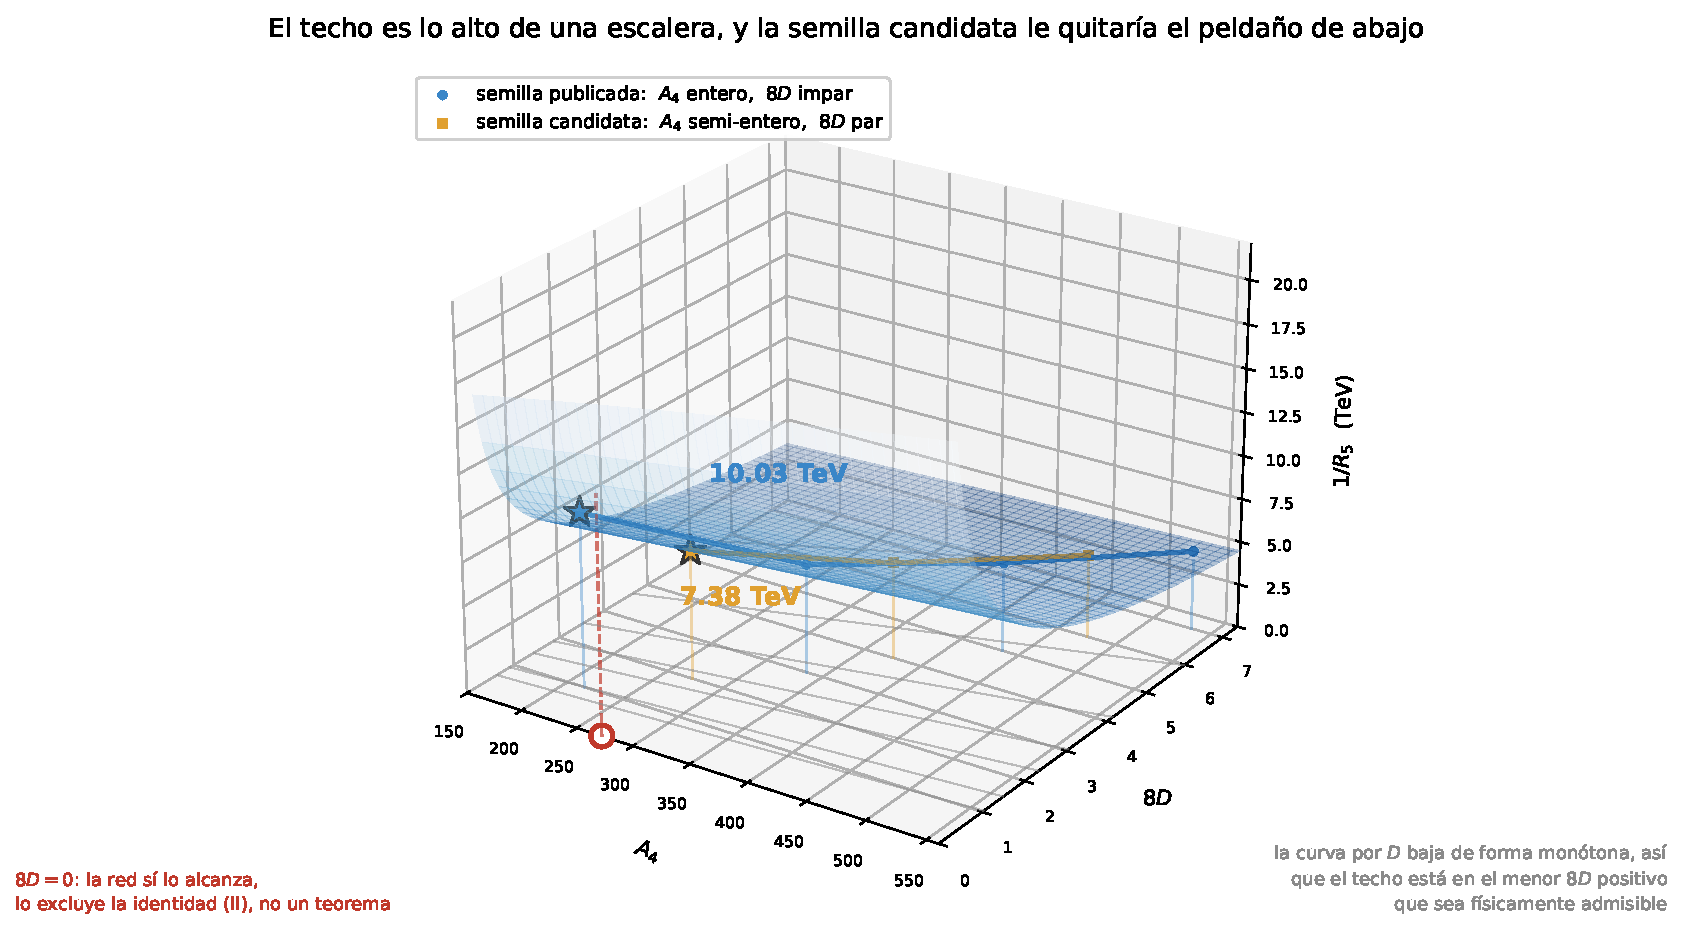
\includegraphics[width=0.92\textwidth]{fig_coset3d_es.pdf}
\caption{\textbf{El techo es lo alto de una escalera, y el desplazamiento candidato le quitaría el peldaño de abajo.} Cada marca es la cota superior certificada sobre $1/R_5$ con ese valor de $8D$ ---el dual LP sobre el cono de momentos, no un óptimo alcanzado---; la superficie de detrás es el objetivo $1/R_5=2\pi m_W/x$, que diverge cuando $8D\to0$. Las dos redes se entrelazan en el plano de base: con los coeficientes de \cite{KM25}, $A_4$ es entero y $8D$ impar, así que la escalera arranca en $8D=1$ y el techo vale $10.03$~TeV; con la semilla \emph{candidata} $A_4$ pasaría a semientero y $8D$ a par, el peldaño $8D=1$ dejaría de existir, y el techo valdría $7.38$~TeV en $8D=2$. La cota no se pierde en ninguna de las dos ramas: baja un peldaño. El círculo hueco en $8D=0$ es la parte honesta: el retículo \emph{candidato} sí llega, y lo que allí lo prohíbe es la identidad~(II), porque $6\mu+A_4>0$ para todo contenido obliga a $x=0$; en el retículo publicado $8D$ es impar y $8D=0$ no está en él en absoluto. Las dos curvas las calcula el mismo programa, que reproduce los $10.03$~TeV publicados antes de que se le permita informar de nada más.}\label{fig:coset3d}
\end{figure}

\textbf{Lo que se pierde no es el número, es la razón.} Con el teorema de los octavos impares,
$8D=0$ era imposible y no había nada que argumentar. Sin él, $8D=0$ \emph{sí} se alcanza en el
retículo ---nueve copias de $\mathbf{28}(+,-)$ llegan--- y lo que lo excluye es que la
identidad~(I) exigiría un $G$ infinito, y ---más limpio, y sin apelar a la optimización--- que la
identidad~(II) lo zanja en una línea. Dice $x^2(6\mu+A_4)=12\zeta(3)D$. Todo multiplete del bulk
aporta una cantidad \emph{no negativa} a $A_4$, que es la propiedad en la que el programa entero ya
se apoya, y el $A_4$ del propio sector gauge vale $-\tfrac{27}{2}$ con la semilla candidata;
mientras tanto $m_h\in[125,127]$~GeV con $g_4=0.63$ deja $6\mu$ entre $481$ y $496$. Así que
$6\mu+A_4>0$ para \emph{todo} contenido, sin excepción y sin salvedad. Entonces $D=0$ obliga a
$x=0$: no hay vacío electrodébil finito sobre esta superficie compatible con la masa del Higgs
medida. Eso es un argumento físico sobre un límite, no un teorema sobre enteros, y es más débil.
Preferimos decirlo a dejar que una cota conserve el rango que tenía cuando la sostenía un teorema.

\emph{De modo que la manera honesta de presentarlo todo no es como una duda sino como una
bifurcación, con las dos ramas costeadas.} La semilla gauge entra en todas partes por dos números,
los pesos $(a,b)$ por par adjunto cargado, y una vez nombrados el resto es contabilidad:

\begin{center}\footnotesize
\rowcolors{2}{white}{softgrey}
\begin{tabular}{lcc}
\toprule
\rowcolor{hdrblue!10} & semilla impresa en \cite{KM25} & candidata $(3{+}1)$ \\
\midrule
pesos $(a,b)$ por par cargado      & $(2,\tfrac12)$        & $(\tfrac32,\tfrac12)$ \\
corchete gauge                     & $(2,4,7)$             & $(\tfrac32,3,6)$ \\
$8D$ del sector gauge              & $-27$, \textbf{impar} & $-18$, \textbf{par} \\
$A_4$ del sector gauge             & $-18$, entero         & $-\tfrac{27}{2}$, semientero \\
$2W$ del sector gauge              & $-3$, impar           & $-3$, impar \\
$32F(0)/\zeta(5)$ del gauge        & $9$, \textbf{impar}   & $18$, \textbf{par} \\
paridad de los tres peldaños $k=0,1,2$ & impar, impar, \textbf{par} & par, par, \textbf{impar} \\
¿está $A_4=0$ en el coset?         & sí, $A_4\in\ZZ$      & no, $A_4\in\ZZ+\tfrac12$ \\
\midrule
\rowcolor{amber!14}hipótesis del Teo.~\ref{thm:eighths} & \textbf{se cumple}  & \textbf{no se cumple} \\
Teo.~\ref{thm:mod6}, $8D\equiv2A_4+3$ & vale               & vale \\
$2W$ impar para todo contenido     & vale                  & vale \\
\rowcolor{amber!14}$|F(0)|\ge\zeta(5)/32$             & vale                  & \textbf{sin demostrar} \\
forma cerrada de Lambert, escalera, núcleo & vale          & vale \\
\midrule
menor $D$ positivo donde cabe el techo & $\tfrac18$        & $\tfrac28$ \\
qué prohíbe $D=0$                  & un teorema            & la identidad~(II) \\
techo dual LP sobre $1/R_5$        & $10.03$~TeV           & $7.38$~TeV \\
óptimo alcanzado; vacío verdadero  & $10.01$; $9.22$~TeV   & sin recalcular \\
\bottomrule
\end{tabular}
\end{center}

\noindent \textbf{Si se recorre el segundo bloque de arriba abajo, la forma del resultado se ve de
golpe.} Unos enunciados que cargan son indiferentes a cuál de las dos columnas sea la buena y otros
no, y la tabla es el único sitio que dice cuál es cuál. Dos filas merecen mirarse dos veces. La cota
sobre el valor $|F(0)|\ge\zeta(5)/32$ no queda sólo reescalada en la rama candidata: se le cae la
\emph{demostración}, porque $32F(0)/\zeta(5)$ da $9$ con una semilla y $18$ con la otra, y a un
entero par no lo aparta del cero el ser entero. Y $A_4=0$, que la rama publicada sí alcanza y
descarta por razones físicas, ni siquiera pertenece al coset candidato: allí $A_4$ es semientero, de
modo que la obstrucción deja de ser un argumento físico y pasa a ser aritmética. \emph{Cuantizado no
quiere decir distinto de cero; cuantizado \textbf{en impares}, sí} ---y para separar esas dos cosas
hizo falta tener delante una segunda semilla.

\noindent \textbf{Y la tabla se lee mucho mejor una vez nombrado el objeto que manda.} No es el
semientero, ni son los tres colores: las dos cosas son propiedades de una semilla que resultan
ciertas. De lo que depende la tabla entera es del \emph{carácter de paridad del punto base gauge
afín}. Sobre la fila que mezcla los dos sectores,
\begin{keyeq}
\begin{equation}\label{eq:chigauge}
  \begin{aligned}
    \chi_{\mathrm{gauge}}(a,b)\;&\equiv\;(2a)+(2b)\ \ (\mathrm{mod}\ 2)\,,\\[2pt]
    \chi_{\mathrm{gauge}}\bigl(2,\tfrac12\bigr)=1\,,\qquad
    &\chi_{\mathrm{gauge}}\bigl(\tfrac32,\tfrac12\bigr)=0\,.
  \end{aligned}
\end{equation}
\end{keyeq}
\noindent Con eso en la mano, cada fila de la tabla se explica sola. La ley módulo seis sobrevive
porque vive en $8D-2A_4$, cuyo resto en el punto base vale $9$ con \emph{las dos} semillas: no ve
nunca a $\chi_{\mathrm{gauge}}$. La imparidad de $2W$ sobrevive porque $2W$ vive en la
\emph{diferencia} de los dos pesos de carga uno, donde un desplazamiento común se cancela. La
imparidad de $8D$ no sobrevive, ni tampoco el hueco por debajo de $|F(0)|$, porque las dos leen
$\chi_{\mathrm{gauge}}$ directamente. \emph{Un carácter, cuatro filas, y ninguna coincidencia
suelta.}

\noindent \textbf{Y una vez nombrado el objeto, la tabla entera es una sola contracción.} Dos
semillas son dos puntos base del mismo retículo afín, de modo que lo que las separa es un
\emph{vector}. En las coordenadas enteras $(2A_4,8D,2U,V,2W)$ vale
\[
  \Delta_{\mathrm{seed}}\;=\;(9,\;9,\;9,\;0,\;0),
\]
derivado de los tres números del corchete gauge y de nada más. Un enunciado escrito como funcional
lineal $\ell$ sobre el contenido sobrevive entonces al cambio de semilla exactamente cuando
$\ell(\Delta_{\mathrm{seed}})$ se anula en el módulo en que ese enunciado está escrito ---y cada
fila de arriba es esa única contracción---. $8D$, $2A_4$, $2U$ y $32F(0)/\zeta(5)$ recogen $9$ cada
uno, que es impar, luego los cuatro voltean. $2W$ recoge $0$, porque lee la \emph{diferencia} de los
dos pesos de carga uno y el candidato los mueve a los dos en el mismo $\tfrac12$. Y $8D-2A_4$ recoge
$9-9=0$ ---no cero \emph{módulo seis}, sino cero---, que es la razón de que el
Teorema~\ref{thm:mod6} sobreviva por un motivo más fuerte que los demás. La misma contracción zanja,
sin ninguna demostración adicional, que la congruencia $\bmod\,8$ $8D\equiv2U$ de la
\eqref{eq:congr5} también sobrevive. \textbf{Así que lo que compra una segunda semilla no es una
segunda columna: es el vector que hay entre las dos}, y con él la lista de qué observables son
ciegos a un desplazamiento del punto base gauge y cuáles lo detectan. Calculado en
\texttt{seed\_\allowbreak shift\_\allowbreak character.py}, que deriva las cinco coordenadas gauge
del corchete y sólo después las contrasta con la tabla, y que lleva un control que puede fallar: una
semilla ficticia que mueva también el peso antiperiódico rompe la invariancia de $2W$, como debe. La Figura~\ref{fig:seedshift} es ese mismo enunciado dibujado. Léase el tercero y la
cota no desaparece en ninguna de las dos ramas: cambia el coset que la sostiene, y con él el
peldaño y el número. \emph{Ése es un resultado más interesante que el que veníamos a contar, y sólo
se ve porque hay dos columnas.} Un artículo de una sola columna no puede decirte cuáles de sus
teoremas se apoyaban en un número heredado.

\begin{figure}[t]\centering
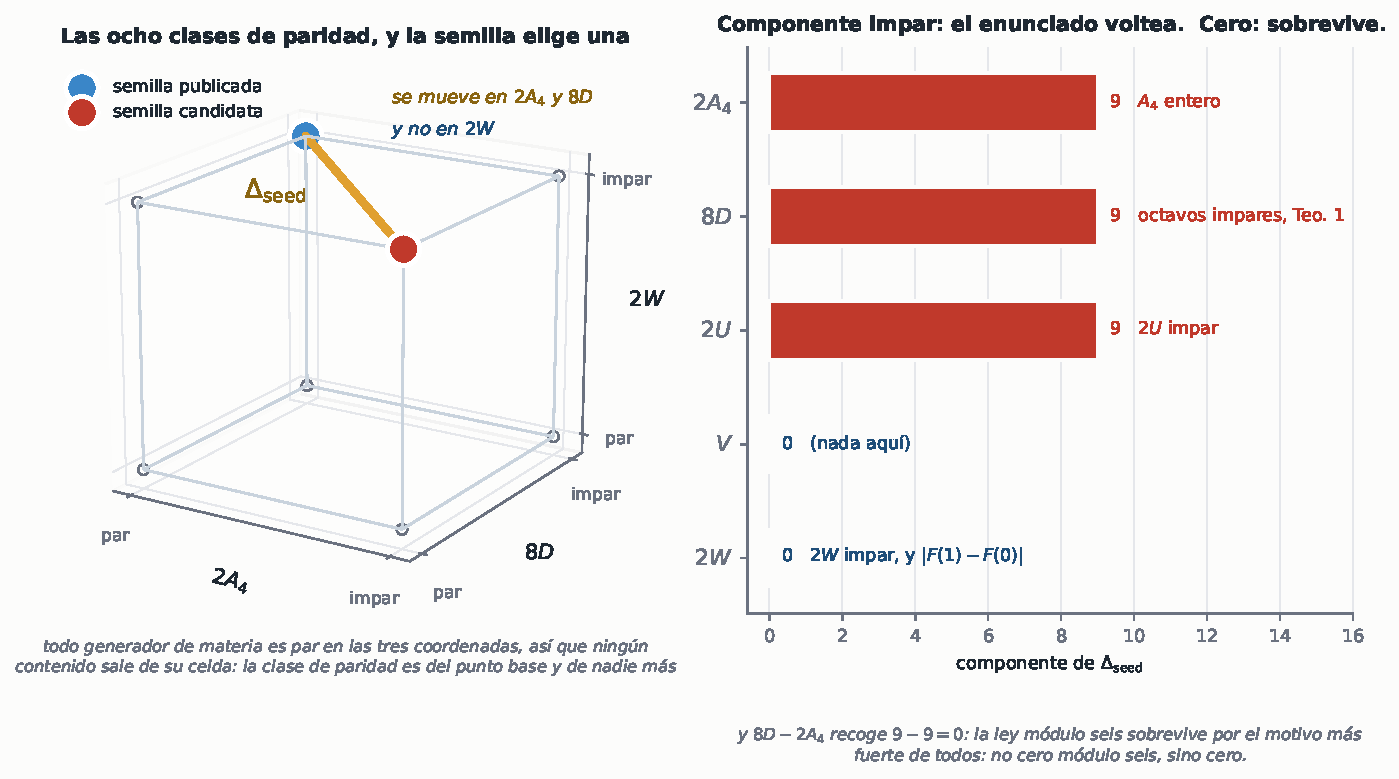
\includegraphics[width=\textwidth]{fig_seedshift_es.pdf}
\caption{\textbf{Dos semillas, dos puntos base, un vector.} \emph{Izquierda:} las clases de
paridad de $(2A_4,8D,2W)$ son los ocho vértices de un cubo, y ningún contenido de bulk puede
salir de la que elige su semilla ---todo generador de materia es par en las tres coordenadas, de
modo que la clase es del punto base gauge y de nadie más---. La semilla que \cite{KM25} imprimen
se sienta en (par,\,impar,\,impar); la candidata de la \S\ref{sec:open}, en
(impar,\,par,\,impar). El segmento ámbar es $\Delta_{\mathrm{seed}}$ leído módulo dos: mueve
$2A_4$ y $8D$ y deja $2W$ donde estaba, que es toda la razón de que la hipótesis del
Teorema~\ref{thm:eighths} falle en la rama candidata mientras el teorema del $2W$ ni se entera.
Es una diagonal de cara y no una arista, porque cambian dos coordenadas y una no.
\emph{Derecha:} las cinco componentes de $\Delta_{\mathrm{seed}}$ y el enunciado que vive en
cada una ---una componente impar voltea su afirmación, un cero la deja en pie---. Dibujada por
\texttt{make\_\allowbreak fig\_\allowbreak seedshift.py}, que toma los ocho generadores de
\texttt{congruences.py} en vez de reteclearlos, y que se niega a dibujar si los ocho no son
pares en esas tres coordenadas y si una semilla ficticia que mueva además el peso antiperiódico
no cae en otro vértice.}\label{fig:seedshift}
\end{figure}

\noindent \emph{Toda ruta de las
Partes~I--VII entra en la cadena causal por el extremo de los coeficientes y va hacia atrás.} Lo
que lo cerraría no es otra prueba de consistencia sino un cálculo en la otra dirección: una suma de
Coleman--Weinberg sobre la torre hexadimensional con estas paridades de orbifold, que dé el peso de
un par con $P_6=-1$ desde su modeado antiperiódico. \textbf{Y ese cálculo no parece existir
publicado}, lo que convierte una debilidad privada en algo que merece hacerse por sí mismo.
\cite{HY04} dan el potencial general de líneas de Wilson a un lazo para $\su{N}$ pentadimensional
sobre $S^1/\ZZ_2$, válido para representaciones y condiciones de contorno arbitrarias ---es lo que
corre la \S\ref{sec:anchor}---. No hemos encontrado contrapartida hexadimensional: el estudio
reciente de $T^2/\ZZ_4$ de \cite{TZ4} escribe potenciales específicos de modelo en vez de una
fórmula general, y no trata $T^2/\ZZ_2$ con dos paridades independientes. Así que el objeto que
falta es el análogo en seis dimensiones de \cite{HY04}, y derivarlo cerraría a la vez el único
eslabón inferido de la cadena de este artículo y aportaría una fórmula que el campo no tiene.
Mientras tanto, la afirmación más fuerte de la \S\ref{sec:collider} ---la \eqref{eq:combchi}, que
lee el peine y por tanto la semilla, y no la \eqref{eq:tulimit}, que no--- tiene una determinación y
ninguna segunda opinión.
\item \textbf{El sector antiperiódico está sin anclar, y no es casualidad.} Toda comprobación
publicada contra la que se pueda anclar una curvatura se sitúa en $B=0$, y sobre ese lugar $\Delta_k=\mathcal{A}_k=S_k$: el momento pesado por
la paridad y el ciego a ella son allí la \emph{misma función}. De modo que ninguna comprobación
publicada puede separar $A$ de $B$, y en particular ninguna pone a prueba el $-\tfrac34$ de
$D=A_2-\tfrac34B_2$ ---el único coeficiente por el que pasan todas las escalas del lado teórico de este
artículo. Esa es la ceguera, y es estructural, no una laguna de lectura: cada una de las tres cosas
que la literatura circundante hace con una paridad se queda en ese lugar. \cite{vGIQ}
construyen la propia traza torcida ---sus (4.42)--(4.43) llevan
$\mathrm{Tr}(\lambda_R T^{A'}_R T^A_R)$, la paridad insertada en la traza, como término de brana
candidato--- y luego demuestran que se \emph{anula} en $S^1/\ZZ_2$, concluyendo su resumen que se
anulan todos los efectos de brana sobre la masa del Higgs. \cite{CCD24} parten la suma por paridad,
pero en $p=5$ y comparando valores en dos puntos del orbifold; las palabras \emph{curvatura},
\emph{segunda derivada}, \emph{Dynkin} y \emph{traza} no aparecen en sus cuarenta y cinco páginas.
(Esa comparación entre dos puntos no nos resulta ociosa: es la \eqref{eq:truevac}, y es la que le
quita ochocientos GeV al techo. Aun así es ciega al desdoblamiento, porque lee el \emph{valor} del
potencial ---el peldaño $p=5$--- y la pregunta del anclaje es sobre el de $p=3$.) Y
\cite{PGY24}, estudiando el mismo potencial de línea de Wilson de forma no perturbativa en
$\mathbb{R}^4\times S^1$, registran que aumentar el número de fermiones equivale a añadir un par de
paridad ---lo cual es exactamente cierto donde ellos lo dicen y exactamente falso aquí, y los dos
momentos dicen por qué en una línea: en nuestro retículo un par de paridad tiene $\Delta=0$ para
cada uno de los cuatro multipletes pero $B\neq0$ para los cuatro, de modo que un par se mueve por el
eje \emph{sin anclar} dejando intacto el momento pesado por la paridad, y una multiplicidad hace lo
contrario. Identificarlos es identificar una dirección que la literatura mide con otra que no.
\textbf{Nadie ha tenido motivo para salir del rincón, porque dentro de él las tres operaciones
coinciden.} Por eso un anclaje para $B\neq0$ hay que calcularlo, no encontrarlo, y es lo más
afilado que a este artículo le falta.

Dos medidas dicen cuánto de afilado, y están en \texttt{anchor\_\allowbreak delta.py}. Primera: el
residuo \emph{no} es función de los momentos ciegos a la paridad. Las filas (1) y (2) de la tabla de
\cite{KM25} tienen los mismos $S_0,S_1,S_2$ hasta el último dígito ---$87.5$, $179.5$,
$707.5$--- y sus residuos difieren en un veinticinco por ciento, algo que ningún ordenamiento
sobre cinco puntos colineales podría haber establecido. Segunda: el desdoblamiento es una
cancelación casi exacta. $D=A_2-\tfrac34B_2$ es $78.000-76.125$ en la fila (1), un residuo del
$2.4\%$, y la palanca que eso da está medida y no estimada: las filas (1) y (2) difieren un uno por
ciento en el desdoblamiento, $78.000-76.125$ frente a $79.000-75.375$, y sus $D$ difieren en un
factor $1.93$ ---de modo que $\alpha_{\min}\sim\sqrt D$ se mueve un $39\%$, el tamaño del propio
residuo. Reescalar el sector
antiperiódico por una sola $\lambda$ no repara las cinco filas, y lo que hay que juzgar es
$\lambda-1$: la perturbación exigida va del $0.2\%$ al $1.4\%$, un factor siete, de modo que
esto se suma a las reparaciones de un parámetro ya excluidas en la Parte~VI. Pero es de un solo
signo y de \emph{ese} orden en todas las filas, lo que cambia lo que el aviso afirma. No es que el
potencial esté equivocado por un factor dos; es que una traza puede estarlo en su segundo dígito,
en el único sitio donde $D$ no tiene holgura.
\item \textbf{Las otras dos congruencias están leídas, y una de ellas ya estaba en este artículo dos
veces.} La \eqref{eq:snf5} da $\ZZ^5/L\cong\ZZ_2\times\ZZ_{72}\times\ZZ_{2592}$. Tal como las
imprime Smith, las dos últimas son ilegibles ---coeficientes de cinco cifras módulo $72$ y
$2592$--- pero $72=8\cdot9$ y $2592=32\cdot81$ son factorizaciones coprimas, así que cada una es en
realidad \emph{dos}. En términos mínimos, y \emph{sobre el coset afín con base en la semilla gauge
que \cite{KM25} imprimen} ---los residuos de abajo son los del coset, no los del subretículo de
materia, que tiene residuo cero en cada una de ellas---, todo contenido de bulk cumple
\begin{equation}\label{eq:congr5}
\begin{aligned}
  8D+2U+2W&\equiv1 &&(\bmod\ 2), &  8D&\equiv 2U+4(2W) &&(\bmod\ 8),\\
  A_4+8D+3(2U)&\equiv V &&(\bmod\ 9), &
  2W&\equiv-\bigl(2A_4+12(8D)+3(2U)\bigr) &&(\bmod\ 32),
\end{aligned}
\end{equation}
junto con $V\equiv0\ (\bmod\ 81)$, que es automática porque $V$ es $81$ por una multiplicidad. Los
cinco módulos multiplican $2\cdot8\cdot9\cdot32\cdot81=373248$, el índice, de modo que esto es
\emph{la descripción completa} de las congruencias del coset y no una muestra. Comprobado en \texttt{congruences.py}
sobre los ocho generadores, el sector gauge, el testigo de la Figura~\ref{fig:vacuum} y las cinco
filas de \cite{KM25}, y contra la forma de Smith en un barrido de $114\,244$ vectores, para que los
enunciados legibles sean el mismo \emph{conjunto} y no un debilitamiento.

Salen dos cosas. \textbf{El carácter de paridad no es ninguno de los factores}: es la sombra módulo
dos \emph{conjunta} de tres de ellos, porque el enunciado $\bmod\,8$ da $8D\equiv2U$, el
$\bmod\,32$ da $2U\equiv2W$, y el $\bmod\,2$ fuerza entonces los tres impares. Así que la
imparidad de $2U$, que la edición anterior de esta lista registraba como un hueco, es
\emph{equivalente} a la de $2W$ ---por una congruencia que no menciona el $-\tfrac72$ en ningún
momento. Y \textbf{el enunciado $\bmod\,9$ es la divisibilidad de este mismo artículo}: reducido
módulo tres dice $A_4+8D\equiv0$, que es a la vez el filtro de paso tres por el que busca la
\S\ref{sec:ceiling} y la observación de la \S\ref{sec:arith} de que las filas de \cite{KM25} dan
$8D+A_4=273,300,198,234,270$, todos divisibles por tres. Son un mismo hecho, y llevar $2U$ compra
una potencia más de tres.

Lo que \emph{no} hacen es mover el techo, y eso es estructural y no cuestión de comprobar casos: la
proyección del retículo de contenidos al plano $(A_4,8D)$ tiene índice exactamente seis ---el mcd
de sus menores $2\times2$---, de modo que la regla módulo seis ya es allí el enunciado completo y
nada que involucre $2U$, $V$ o $2W$ puede recortar más el plano. Lo que prohíban, lo prohíben
dentro de una fibra. La única escapatoria sería un vértice cuya fibra vacíen, y los tres sobre los
que discute este artículo, $A_4=104,212,215$ en $8D=1$, se limitan a fijar $2U$ en una clase módulo
tres, que los ocho multipletes realizan. Qué \emph{significa} un $2U$ impar sigue por tanto
abierto, pero ya no es un hueco distinto del teorema del $2W$.

\emph{Y la proyección a cuatro coordenadas viene incluida.} La edición anterior de la tabla de
límites registraba que las condiciones tras el $\ZZ^4/L\cong\ZZ_{18}\times\ZZ_{648}$ de la
\eqref{eq:snf} estaban calculadas pero no escritas; eliminar $2W$ de la \eqref{eq:congr5} las
escribe. Sobre el retículo de materia, $8D\equiv0\ (\bmod\ 2)$, $8D-2U\equiv0\ (\bmod\ 8)$,
$A_4+8D+3(2U)-V\equiv0\ (\bmod\ 9)$ y $V\equiv0\ (\bmod\ 81)$ ---con residuo \emph{cero} en cada
una, como le toca a un subgrupo---. Añadir el punto base gauge que \cite{KM25} imprimen lo traslada
al coset afín, y es \emph{ahí} donde un contenido lee $1,4,0,0$: en un
contenido ---y las dos lecturas difieren de verdad en la segunda, donde el $4(2W)$ sobrevive sólo
porque $2W$ es impar. Índice $2\cdot8\cdot9\cdot81=11664=18\cdot648$, confirmado cerrando el
subgrupo de $(\ZZ/32)^4$ y $(\ZZ/81)^4$ por fuerza bruta y no fiándose de la eliminación.
Sobreviven otras dos preguntas. ¿Es \emph{normal} el semigrupo levantado? En la proyección lo es: ningún punto del
cono con la congruencia queda fuera de alcance, medido hasta $A_4=420$; si el levantamiento tiene
agujeros, son contenidos que toda ley visible permite y que ningún bulk puede construir. Y cuál es
la función de partición vectorial $N(A_4,8D,2U,V)$, que debería ser cuasi-polinómica en las cámaras
del cono y convertiría las degeneraciones de la Figura~\ref{fig:collapse} de medida en fórmula.
\item \textbf{¿Dónde muerde el tercer mínimo?} La edición anterior de esta lista preguntaba si
$W>0$ es suficiente además de necesaria, y proponía el programa semi-infinito como forma de
averiguarlo. La \S\ref{sec:ceiling} lo corre ya, y la respuesta tiene dos mitades. En el peldaño
que decide el techo el programa genera exactamente un corte, el de $y=1$, así que allí $W>0$ es
toda la condición de vacío verdadero y \eqref{eq:ceilingtrue} no necesita cribado ninguno. Pero un
contenido invisible para los dos puntos simétricos sí existe ---\eqref{eq:semiinf} exige un segundo
corte sobre $8D=3$, y la \S\ref{sec:ceiling} lo coloca en la holonomía racional exacta $y=2/3$,
donde la profundidad es el funcional en forma cerrada $-\tfrac{121}{81}\zeta(5)[C_1+C_2+C_4]$---, de
modo que el fenómeno es real, es exacto, y lo único que le pasa es que no llega al peldaño que
decide. Lo que queda abierto es más pequeño y más nítido: ¿hay algún peldaño en el que un corte
distinto del de $y=1$ mueva el \emph{techo} en vez de un vértice interior? Y dónde se sientan los
\emph{demás} cortes es ya un negativo medido y no una pregunta sin intentar: a lo largo de $6560$
contenidos, los $2956$ minimizadores interiores quedan apenas $1.05$ veces más cerca del esqueleto
racional $\{1/3,1/2,2/3\}$ que el azar. El $y$ donde se sienta el tercer mínimo de un contenido
sigue debiendo leerse de sus cargas igual que se lee $\alpha_{\min}$, y no se lee ---y ahora consta
que la holonomía racional más próxima no es la forma de leerlo.
\item \textbf{Una cota del resto uniforme en el peldaño.} La \eqref{eq:rigorousceiling} está
demostrada sobre los primeros setenta peldaños impares y no más allá, y la razón se puede medir: la
mordida relativa de la cota, $\delta/\hat x$, sube de $2.5\times10^{-4}$ en $8D=1$ a
$9.0\times10^{-1}$ en $8D=1201$, de modo que se afloja más deprisa de lo que cae el techo truncado y
acaba por no certificar nada. Eso es un defecto de la \emph{cota}, no del techo ---la
\eqref{eq:slope} demuestra $M(k)\le6268$~GeV en todo peldaño $k\ge3$ sin barrido ninguno. Lo que falta
es una cota de $|R'_j(\hat x(k))|$ que decaiga al menos tan rápido como la curvatura $\propto k$, y
eso cerraría la \eqref{eq:rigorousceiling} para todo $k$ en una línea. Los restos por multiplete son
colas explícitas de Li$_5$, así que esto parece un ejercicio de acotar
$\sum_{n>N}\sin(nc\hat x)/n^4$ uniformemente cuando $\hat x\to\hat x_\infty$ y no un problema
abierto; no lo hemos hecho.
\item \textbf{El margen entre el $215$ y el $212$ es menor que el desarrollo que lo produjo.} Una
parte en $10^{4}$, frente a una forma cerrada buena al $0.13$--$0.62\%$. El remedio no son más
dígitos sino las identidades corregidas: rehacer la eliminación \emph{sin} tirar el resto $R$ da
$x^2(6\mu+A_4)=12\zeta(3)D-18R'/x+6R''$ y una corrección análoga en la (I), y la
\S\ref{sec:closed} acaba de establecer que $R$ es una cola convergente con cota rigurosa. Correr el
programa entero sobre intervalos certificados para $x$ en vez de sobre la superficie truncada
convertiría los $10.01$~TeV de afirmación sobre la superficie algebraica en afirmación sobre el
potencial polilogarítmico. Es lo más valioso que queda en este artículo.
\item \textbf{Qué convertiría la sensibilidad del recast en una exclusión. Ahora una sola cosa, y
el programa de cierre sobre datos públicos queda agotado.} Se han corrido tres cierres y ninguno
de ellos es el paso que falta. \emph{Los límites observados}: apuntada al límite publicado de
singlete de \cite{CMSangular} sobre su propia selección, la maquinaria devuelve $17.5$ frente a
$17$~TeV y $29.5$ frente a $37$. \emph{Los esperados}: un conjunto Asimov del Modelo Estándar por
nuestro propio $\chi^2$ devuelve $1.08$ y $0.85$ frente a los $18^{+20}_{-2}$ y
$34^{+8}_{-5}$~TeV esperados de \cite{CMSangular}, lo bastante cerca de los $1.03$ y $0.80$
observados como para que el hueco sea el método y no este conjunto de datos. \emph{Y la
plantilla}, que era la más afilada de las tres preocupaciones: el
benchmark del cierre debería ser el operador vectorial $VV$ y no sólo $LL$: la torre es
$(\bar q\gamma^\mu T^aq)^2$, que ve las dos quiralidades, mientras que los $17$ y $37$~TeV son
de mano izquierda, y los límites $VV$ publicados se comportan lo bastante distinto ---el
constructivo llegando a unos $50$~TeV, el destructivo desarrollando regiones desconectadas donde
la interferencia se cancela contra $1/\Lambda^4$--- como para que concordar con uno diga poco
del otro. La maquinaria está puesta ---la base de operadores de \cite{CIJET} es la quiral de su
ec.~(2), luego $VV$ es $\lambda_1=\lambda_3=\lambda_5$ donde el cierre ya corrido es $\lambda_1$
solo---. \textbf{Esa corrida ya está hecha, y zanja la preocupación en lugar de confirmarla.}
Emparejando selección contra selección, en el lado constructivo donde \cite{CMSangular} publican
límite para los dos operadores, el cociente del cierre pasa de $0.80$ a $0.78$ en su propia
selección de interacción de contacto, y de $0.69$ a $0.66$ sobre las siete bandas de masa. Dos
selecciones, el mismo sentido, y \textbf{dos o tres puntos las dos veces}. \emph{De modo que la
quiralidad de la plantilla no es de lo que está hecho el déficit del cierre} ---lo que conviene
saber, porque era la explicación más plausible disponible y ahora es la menos---. Lo que el
emparejamiento \emph{no} hace es darle al déficit un tamaño único: vale $0.78$ en la selección de
contacto emparejada y $0.66$ sobre las siete bandas, de modo que la discrepancia depende de la
selección y lo único estable es el paso de $LL$ a $VV$. En el lado
destructivo no hay con qué emparejar: \cite{CMSangular} no publican límite $VV$ ahí. Y el déficit
sigue siendo lo que era, \textbf{precisión del cierre y no un sistemático multiplicativo
transferible}; medirlo dos veces no lo convierte en una banda. \textbf{Lo que queda es un solo
paso, y es el que cuesta}:
el límite
debería ponerse como lo pone \cite{CMSangular}, con verosimilitudes de Poisson a nivel detector,
parámetros \emph{nuisance} perfilados y $CL_s$.
Hasta entonces la \eqref{eq:tulimit} es una sensibilidad y así está escrita. \textbf{Y a su lado
hay un segundo sistemático, de otra clase y sin medir}: la línea base es la QCD a orden
siguiente al siguiente al dominante de \cite{CMSangular}, mientras que la deformación de la
torre se valida contra \cite{CIJET} a orden dominante, de modo que las dos entran en la
\eqref{eq:chisq} a órdenes distintos. El $0.2\%$ es un cierre de implementación de la
interferencia a orden dominante y no un enunciado sobre el factor $K$ que falta; cuánto movería
a la \eqref{eq:tulimit} una deformación a NLO no se mide aquí, y es la más barata de contestar
de las preguntas de colisionador que quedan abiertas.

\item \textbf{La literatura de holonomía térmica no está barrida.} La \S\ref{sec:parity} hace de los
dos problemas una sola familia; esa literatura tiene $V''(0)\propto T(R)$ como material de manual y
las trazas proyectadas por $\ZZ_2$ como contabilidad natural, así que es el sitio con mayor
probabilidad a priori donde el puente ya podría existir. Queda nombrado aquí como compuerta abierta,
no como nulo.
\item \textbf{Dos lazos.} El mapa calculado aquí es un mapa a un lazo. A dos lazos el potencial ve
más del contenido ---un peso $W(w,w')=\sum_a|\langle w|T^a_R|w'\rangle|^2$ en lugar de una
multiplicidad--- y a qué es ciego ese segundo peldaño se puede decidir sin ninguna integral de lazo.
\item \textbf{Unificación de los acoplos gauge, que es su propia pregunta abierta.} \cite{KM25}
cierran pidiéndola: $\su3_C$ y $\su4$ están dentro de un mismo $\su7$, de modo que los acoplos han de
encontrarse donde se restaura la simetría, y dejan el análisis a un lazo para trabajo futuro. La
mitad queda zanjada aquí y no cuesta nada: por debajo de $1/R_5$ la teoría es el Modelo Estándar,
luego $\alpha_2^{-1}-\alpha_3^{-1}$ vale $19.2$ a $2$~TeV y $18.2$ en el techo certificado ---apenas
se mueve a lo largo de todo el rango permitido, porque el correr cuatridimensional dispone de menos
de cinco e-folds y cierra la diferencia a razón de $0.61$ por e-fold. \textbf{Toda la carga recae por
tanto sobre la torre de Kaluza-Klein}, y el techo de la \S\ref{sec:ceiling} no es un espectador: fija
dónde puede empezar esa torre. La otra mitad ---si la torre de $\su7$, cuyos niveles la proyección
del orbifold deja incompletos, puede cerrar $18.2$ antes de que se acabe la perturbatividad--- es un
cálculo, no una opinión, y es el artículo siguiente natural.
\item \textbf{¿Tiene la dimensión del teorema un enunciado general?} La \S\ref{sec:arith} muestra que
la protección no está en la clase pentadimensional que cubre la fórmula de \cite{HY04} ---$\su{N}$
sobre $S^1/\ZZ_2$ con una sola fase de Wilson, donde todos los peldaños son pares y $D=0$ se alcanza
con tres multipletes---, mientras que aquí los peldaños por debajo del cuarto momento son impares. El
mecanismo es el carácter de paridad \eqref{eq:chigauge} del punto base gauge ---no un semientero
suelto---, y la segunda paridad independiente es la que aporta el carácter afín de más que \emph{puede}
hacer impar un peldaño ---en esta construcción, que es hasta donde alcanza un solo modelo---. Si \emph{peldaño impar $\Leftrightarrow$ segunda paridad} es un teorema ---a lo largo de
los $T^2/\ZZ_N$, y en siete dimensiones--- no lo zanja un solo modelo.
\item \textbf{¿Organiza los contratérminos el reparto periódico/antiperiódico?} En el polo, sí:
\eqref{eq:ladderab} manda la mitad antiperiódica a cero en $p=1$, de modo que el punto de
ramificación lo alimenta el momento periódico y sólo él, y periódico significa conservador del
momento. Si eso coincide con la estructura divergente localizada en el bulk, y el sector de paridad
complementario alimenta los términos de borde, es una interpretación y no una consecuencia del
peldaño: hace falta un cálculo explícito de contratérminos. Si el mismo reparto funciona lejos del polo ---una mitad alimentando el
operador de bulk con derivadas superiores, la otra el localizado en el borde--- es lo que abre la
correspondencia de Hurwitz de la \S\ref{sec:novel} y no responde.
\item \textbf{El retículo, contado.} El retículo de multipletes con su congruencia es un cono
racional intersecado con un subretículo afín, así que el número de contenidos a $(A_4,8D)$ fijo es
una función de partición vectorial, y el Teorema~\ref{thm:mod6} aporta una condición de clase
residual de las que sostienen su estructura cuasipolinómica por cámaras. \emph{No} que seis sea el
cuasiperiodo mínimo: eso aquí no se demuestra, y una congruencia sobre el retículo es un enunciado
más débil que un periodo. Es maquinaria que
este artículo usa sólo en su mitad poliédrica.
\end{itemize}

% ===================================================================
\section*{El libro de cuentas}
\addcontentsline{toc}{section}{El libro de cuentas}

% \scriptsize AQUI, y \footnotesize en la edicion inglesa: UNA sola muesca de diferencia, en un
% solo bloque, y es la UNICA asimetria de composicion entre las dos.  Es deliberada y se midio.
% Esta edicion lleva alrededor de un 4 % mas de texto renderizado que la inglesa, porque el
% castellano se estira, asi que a igualdad de ajustes salia a 42 paginas contra 41.  Un ajuste
% SIMETRICO ya no puede cuadrarlas: medido sobre los PDF, a la inglesa le quedaban 17 lineas de
% margen en su ultima pagina y a esta le sobraban 16, asi que la ventana de ahorros que arregla
% una sin hundir la otra esta vacia.  Y apretar la prosa castellana habria significado recortar
% contenido, contra el convenio de la casa, que es traduccion COMPLETA y no resumen.  Asi que la
% diferencia se absorbe donde menos se lee, en el cuerpo del libro de cuentas.  Si vuelves a
% tocar el abstract o el libro de cuentas, recompila LAS DOS y comprueba que siguen a la par.
\begingroup\scriptsize
\begin{longtable}{p{0.62\textwidth}p{0.31\textwidth}}
\toprule
\rowcolor{okgreen!12}\textbf{Establecido, y cómo} & \textbf{Dónde}\\
\midrule
\endfirsthead
% El libro cambia de veredicto segun avanza --- establecido, corregido, retirado, abierto ---, asi
% que repetir la cabecera verde "Establecido" en las paginas de continuacion pondria esa palabra
% encima de filas retiradas o abiertas. Lo hacia, hasta que se arreglo. La cabecera de continuacion
% es neutra.
\toprule
\textbf{El libro de cuentas, continuación} & \textbf{Dónde}\\
\midrule
\endhead
$\amin$ en forma cerrada: mediana del $0.13\%$ sobre $272$ contenidos, $0.209\%$ sobre las cinco
filas publicadas, contra nuestra propia minimización numérica del mismo potencial &
\S\ref{sec:closed}; el control sin logaritmo falla entre $+104$ y $+174\%$\\
$F''(\amin)=\pi^2[2\zeta(3)D-A_4x^2/6]$: el logaritmo y $G$ se cancelan en el punto estacionario, de
modo que las dos columnas de su Tabla~1 se siguen de $(D,A_4)$ sin minimización ---con
\emph{nuestros} valores de las dos, no con su columna $\amin$ publicada &
\S\ref{sec:mh}\\
Las dos identidades sin logaritmo, verificadas a $6\times10^{-14}$ &
\S\ref{sec:ceiling}, ec.~\eqref{eq:two}\\
$8D$ es un entero impar, luego $D\ne0$ y \emph{el punto simétrico} nunca es marginal ---
\textbf{condicionado a la semilla gauge de \cite{KM25}}; la mitad de materia del argumento no lo
está & \S\ref{sec:arith}, \S\ref{sec:open}; $4096$ asignaciones de paridad, ningún contraejemplo\\
$8D\equiv2A_4+3\pmod6$, a partir de $c^4\equiv c^2\pmod3$ --- \textbf{vale con cualquiera de las
dos semillas} & \S\ref{sec:arith}; las cinco filas publicadas y los ocho generadores\\
$|F(0)|\ge\zeta(5)/32$, con la cota alcanzada ---\textbf{condicionado a la semilla gauge de
\cite{KM25}}: lee la \eqref{eq:chigauge} igual que los octavos impares, y con la semilla candidata
$32F(0)/\zeta(5)$ es par & \S\ref{sec:arith}, \S\ref{sec:open}\\
La escalera es geométrica de razón $c^2/4$, con la carga dos como punto fijo; y
$O(5)-O(3)=4[O(3)-O(1)]$ siempre que no se abra un tercer modo & \S\ref{sec:ladder}; $4096$
asignaciones, y una predicción confirmada en los ocho multipletes\\
La escalera sigue más allá de su propio polo hasta $p=-1,-3,\dots$, donde $\zeta$ es racional: existe
exactamente un logaritmo, a orden $x^4$, y el resto es una cola convergente para
$|\alpha|<1/c_{\max}$ & \S\ref{sec:closed}; razones de términos $(c\alpha)^2$ y $(c\alpha/2)^2$, con
controles pasados los dos radios\\
$A_4=0$ obliga a $8D\equiv3\pmod6$, luego la rama analítica no puede alcanzar el cuanto $8D=1$; y en
esa rama ningún contenido tiene a la vez $D>0$ y $W>0$ ---\textbf{dicho sobre la semilla que
imprime \cite{KM25}}, porque en el coset candidato $A_4\in\ZZ+\tfrac12$ y $A_4=0$ no aparece
siquiera--- & \S\ref{sec:arith},
ec.~\eqref{eq:analytic}; once soluciones base, un multiplete libre, aritmética exacta, y falla por
un paso\\
$2W$ es un entero impar, luego $|F(1)-F(0)|\ge\tfrac{31}{32}\zeta(5)$: en \emph{este} modelo los dos
puntos simétricos nunca son degenerados, luego nunca son descripciones equivalentes de un mismo
orbifold ---al contrario que en los de \cite{CCD24}, donde sí lo son &
\S\ref{sec:ceiling}, ec.~\eqref{eq:nevermarginal}; \textbf{no} es el mismo semientero que el del
Teorema~\ref{thm:eighths}, como decía una versión anterior de esta fila: $2W$ lee la
\emph{diferencia} de los dos pesos de carga uno, así que vale con \emph{las dos} semillas gauge
allí donde la imparidad de $8D$ no. Comprobado en $3003$ contenidos\\
$M_{\mathrm{KK}}^2$ se sienta en un peine aritmético de paso $8\pi^2m_W^2/(\zeta(3)\,8D)$, necesario y
no suficiente & \S\ref{sec:pred}, ecs.~\eqref{eq:comb}--\eqref{eq:comb2}\\
El cambio de paridad en carga dos es el único sin logaritmo, con firma $(-7,-16,-100/3)$ &
\S\ref{sec:ladder}, ec.~\eqref{eq:c2flip}\\
$1/R_5\le10.03$~TeV para contenido de bulk arbitrario, por un dual racional exacto ---\textbf{con la semilla que \cite{KM25} imprimen} &
\S\ref{sec:ceiling}; domina a los $1097$ contenidos en ventana hallados hasta $N=14$\\
$G=\tfrac{25}{12}A_4-U\ln2-V\ln3$ levanta el contenido a un retículo \emph{tetradimensional} con
$\ZZ^4/L\cong\ZZ_{18}\times\ZZ_{648}$, donde el vértice $(215,1)$ de la relajación está vacío y la
cota se afila a $10.01$~TeV
\emph{alcanzada} & \S\ref{sec:ceiling}, ecs.~\eqref{eq:snf}, \eqref{eq:ceilinginteger}; rango y
factores invariantes en \texttt{lattice\_\allowbreak rank.py} y, por vía independiente, en Sage,
\texttt{lattice\_\allowbreak rank.sage}; el máximo sobre un conjunto factible finito a cincuenta
dígitos, el testigo reconstruido por \texttt{moments()}\\
El resto más allá de tres peldaños va acotado, no estimado, y es él mismo \emph{lineal} en las
multiplicidades, así que viaja dentro del propio dual del certificado: $1/R_5\le10.037$~TeV sobre el
potencial sin truncar sobre los primeros $70$ peldaños impares, un $0.025\%$ por encima del
certificado truncado; pasados ésos la cota del resto se afloja y no certifica nada & \S\ref{sec:ceiling},
ecs.~\eqref{eq:remainder}, \eqref{eq:rigorousceiling}; $32$ contenidos $\times$ cuatro $\alpha$, cero
violaciones, y la cota se niega en $u\ge1$\\
El criterio de estabilidad de \cite{CCD24}, sumado sobre un contenido, es un cuarto funcional
\emph{lineal}, así que cabe dentro del mismo programa entero; imponerlo da $1/R_5\le9.22$~TeV sobre
la superficie de tres peldaños, alcanzado, y su testigo sobre el potencial exacto da $9157$~GeV.
\textbf{El criterio es suyo; sólo su uso aquí es nuevo} &
\S\ref{sec:ceiling}, ecs.~\eqref{eq:truevac}--\eqref{eq:ceilingtrue}; cerrado contra exacto a
precisión de máquina en seis contenidos. Sin truncar no es todavía un número único, ni un intervalo:
el testigo da $9157$~GeV, los primeros $70$ peldaños impares quedan acotados por $10.037$~TeV, y una
cota sobre \emph{todos} los peldaños está abierta ---\S\ref{sec:open}\\
El escape de la Parte~VI cuesta exactamente $10/8$ de $D$, luego poder pagarlo fuerza $8D\ge11$ y
baja el techo a $3.97$~TeV ---el contenido de mayor jerarquía es el que no puede pagar &
\S\ref{sec:ceiling}, ec.~\eqref{eq:escapeceiling}; el mismo dual, y $857$ de los $1097$ pueden\\
Nuestra maquinaria reproduce el criterio de \cite{vGIQ}, sus tres números críticos de sabores, su
mínimo de $\su2$ y el corchete entero de teoría de grupos de su fórmula de curvatura &
\S\ref{sec:anchor}; residuo $2/\pi^2$ con ocho dígitos, un convenio puro\\
Una sensibilidad nominal de recast de $1/R_5>10.86$~TeV sólo con el factor de forma espacial
---sin anchura, sin $\mathrm{BR}(G_n\to jj)$---, que deja la rama del escape de $3.97$~TeV un
factor tres por debajo & \S\ref{sec:collider}, ec.~\eqref{eq:tulimit}; contra la covarianza
$77\times77$ de \cite{CMSangular} con la escala perfilada, sobre una maquinaria que devuelve su
propio límite de contacto como $17.5$ frente a $17$ y $29.5$ frente a $37$~TeV, y el
\emph{esperado} como $1.08$ y $0.85$ ---de modo que el hueco con su $CL_s$ es el método y no una
fluctuación de estos datos---. Reponer el canal $s$, con la anchura total perfilada y su peor caso
en $\Gamma_{\mathrm{exotic}}=0$, cuesta un $1.03\%$\\
Leído en los dientes del peine de techos por peldaño y no en una masa cualquiera, el recast dice que la
región permitida no está en parte desfavorecida sino entera: el techo por peldaño más alto al que
puede llegar un contenido del bulk con la semilla que \cite{KM25} imprimen, $10.03$~TeV en $8D=1$, cae en $\Delta\chi^2=12.0$ frente a un
umbral de $3.84$, y el diente siguiente en $\Delta\chi^2=244$ & \S\ref{sec:collider},
ec.~\eqref{eq:combchi}, Fig.~\ref{fig:chi2}; nominal, del mismo $\chi^2$ gaussiano, y así dicho\\
\midrule
\rowcolor{hdrblue!10}\textbf{Corregido aquí, y dejado a la vista} & \textbf{Por qué}\\
\midrule
``$1/R_5\le2.18$~TeV con la ventana del Higgs'' & eso es una cota sobre el \emph{tamaño} del
contenido ($\le6$ multipletes), no sobre el modelo. Con ocho multipletes se llega a $9.14$~TeV.
\S\ref{sec:ceiling}\\
``en el momento cero la marginalidad es alcanzable'' & cierto con recuentos de componentes puros,
falso aquí ---pero no por la razón que daba esta fila. Lo que lo prohíbe es el carácter de paridad
\eqref{eq:chigauge} del punto base gauge, ni un semientero suelto ni la sexta dimensión por su
cuenta: la semilla candidata es igual de hexadimensional y tiene $\chi_{\mathrm{gauge}}=0$.
\S\ref{sec:arith}, \S\ref{sec:open}\\
El $1.94$ y el $1.20$ de la \S7 de la Parte~VI citados como un rango & son medias de grupo ($n=2$ y
$n=3$); el rango fila a fila es $1.03$--$2.08$, y la \S\ref{sec:pred} usa el rango\\
``el techo se alcanza en $(A_4,8D)=(215,1)$'' & el dual lo \emph{certifica} ahí y el retículo
\emph{llega}, pero ningún contenido de ningún tamaño puede pagarlo en $G$ ---corto por $0.067$ en un
presupuesto de $681$. El vértice de debajo sí: $10.01$~TeV en $(212,1)$, alcanzado y con testigo.
\S\ref{sec:ceiling}, ec.~\eqref{eq:ceilinginteger}\\
``dieciséis contenidos con $A_4=0$'' & diecisiete. La enumeración topaba la multiplicidad en cuatro
por multiplete mientras la frase decía seis; el que faltaba tiene $D<0$, así que los ``cinco con
$D>0$'' siguen en pie. \S\ref{sec:arith}\\
``el desarrollo es asintótico'' & es convergente para $|\alpha|<1/c_{\max}=1/3$, y todo $\alpha$ que
se usa aquí queda dentro por un factor de al menos $2.7$. \S\ref{sec:closed}\\
``$A_4=0\Rightarrow m_h\le29.6$~GeV, un margen exacto'' & ese número salió de evaluar la forma
cerrada en $\alpha\simeq0.89$, un factor $2.7$ \emph{fuera} de su propio radio. Retirado y
sustituido por la \eqref{eq:analytic}, que no usa desarrollo ninguno. \S\ref{sec:arith}\\
``los $9.16$ de la enumeración frente a los $10.03$ del certificado son el hueco entre una
relajación y su retículo'' & no lo son: son la condición de vacío verdadero, que la enumeración
imponía en silencio a través del minimizador global y que el certificado no imponía en absoluto.
Con nombre, son $9.22$~TeV alcanzados. \S\ref{sec:ceiling}\\
``restituir las anchuras baja el coeficiente de contacto de la torre un $2.55\%$, así que
$\Lambda_8$ queda bajo un $1.3\%$'' & no hay anchura que restituir. En los canales espaciales cada
modo está bajo su umbral de dos partones, así que el propagador es real; el delator es que el
desplazamiento no se apaga cuando $t\to0$. Retirado, y la torre sumada exacta en su lugar,
\eqref{eq:resum}. \S\ref{sec:collider}\\
``los $3.97$~TeV están ya dentro de la región excluida'' & las exclusiones citadas son para una
resonancia \emph{estrecha} y este objeto tiene $\Gamma/M\simeq0.16$; el canal $s$ necesita además
un cociente de desintegración que el modelo no fija. Sensibilidad, no exclusión ---y el recast
angular, ya hecho, no cambia esa palabra: es un $\chi^2$ gaussiano sobre datos desplegados y no el
$CL_s$ a nivel de detector de \cite{CMSangular}. \S\ref{sec:pred}, \S\ref{sec:collider}\\
\midrule
\rowcolor{warmred!14}\textbf{Retirado, y dejado a la vista} & \textbf{Por qué}\\
\midrule
``el corchete de la tabla gauge es el número de colores, luego el teorema de paridad y la muerte de
la obstrucción son un mismo producto'' & cierto en su asignación, falso en $3872$ de $4096$. Una
coincidencia en un punto. \S\ref{sec:novel}\\
``la jerarquía es una casi cancelación cuantizada entre bulk y brana'' & medido antes de escribirlo:
un efecto del $10\%$, no del $90\%$. Lo que sobrevive es un enunciado de percentil sobre sus cinco
filas. \S\ref{sec:novel}\\
``el mecanismo del reparto por paridad es nuestro'' & está publicado en $p=5$ \cite{CCD24}. Sólo se
reclaman el peldaño $p=3$ y sus consecuencias. \S\ref{sec:ladder}, \S\ref{sec:novel}\\
``el criterio de vacío verdadero de la \S\ref{sec:ceiling} es nuestro'' & no lo es: la \S2.2 de
\cite{CCD24} lo enuncia, demuestra sus identidades y saca su regla de signos. Sólo se reclama su uso
dentro del programa entero. \S\ref{sec:ceiling}, \S\ref{sec:novel}\\
\midrule
\rowcolor{amber!14}\textbf{Abierto, y enunciado como abierto} & \textbf{Por qué}\\
\midrule
Nuestro ensamblaje no reproduce la columna $\amin$ de su Tabla~1 & Parte~VI \S7; la \S\ref{sec:anchor}
estrecha el lugar hasta el diccionario del modelo, pero no lo cierra\\
El sector antiperiódico está sin anclar & ningún anclaje de \emph{curvatura} publicado e
independiente pone a prueba $B\neq0$; los repartos de paridad que existen se quedan en el peldaño
del valor, $p=5$. En $B=0$, $\Delta$ y $S$ coinciden. \S\ref{sec:anchor}\\
El mínimo adjunto de $\su3$ de \cite{vGIQ}, $0.29$, frente a nuestro $1/3$ exacto & el control del
centro favorece al nuestro; no está demostrado, así que no se llama erratum. \S\ref{sec:anchor}\\
Qué \emph{significa} físicamente un $2U$ impar & la congruencia ya está escrita,
\eqref{eq:congr5}, y ata $2U$ a $2W$; falta la interpretación. \S\ref{sec:open}\\
¿Es normal el semigrupo levantado? & el proyectado sí lo es, hasta $A_4=420$. \S\ref{sec:ceiling}\\
¿Dónde muerde el tercer mínimo? & zanjado donde se decide la cota: en $8D=1$ el programa
semi-infinito sólo genera el corte de $y=1$. En $8D=3$ exige uno, y ése es exacto en $y=2/3$, así
que el fenómeno es real y no llega. Dónde se sientan los \emph{otros} cortes es un negativo
medido: los minimizadores interiores no se apiñan en el esqueleto racional.
\S\ref{sec:ceiling}\\
La literatura de holonomía térmica no está barrida & la \S\ref{sec:parity} la convierte en la misma
familia, de modo que es el sitio con mayor probabilidad a priori donde podría existir el puente.
\S\ref{sec:open}\\
¿Es la sensibilidad del recast una exclusión? & los $10.86$~TeV, y los $13.75$ en su propio rango
de masas para interacciones de contacto, pasan de $9.09$ y de $10.03$. Pero un $\chi^2$ gaussiano
sobre datos desplegados no es su $CL_s$ a nivel detector, y los dos benchmarks del cierre difieren
por la física de la interferencia y no por una calibración. Los cierres observado y esperado
diagnostican una discrepancia del orden del diez al veinte por ciento en $\Lambda$ sobre la
selección de contacto emparejada, y mayor sobre las siete bandas; ninguno de ellos define una
incertidumbre trasladable. Cerrar la
verosimilitud es lo que zanjaría el techo. \S\ref{sec:collider}\\
Toda escala del lado teórico arrastra el residuo del anclaje & \S\ref{sec:setting}; el recast de
colisionador no, porque no pasa por $\amin$. El techo se cita con él en la \S\ref{sec:pred}\\
El residuo del anclaje es una \emph{tendencia}, no dispersión, y los dos techos quedan fuera del
rango que la mide & ordenados por $D$ los cinco cocientes son monótonos, $2$ de $120$
emparejamientos, $p=0.017$; pero $A_4$ los ordena igual de bien y cinco filas no pueden separar los
dos momentos. El techo se alcanza en $D=1/8$ frente a un $[1.125,3.625]$ anclado, y el techo del
escape en $A_4=727$ frente a $[189,271]$. \S\ref{sec:setting}, \S\ref{sec:pred}\\
\bottomrule
\end{longtable}
\endgroup

\section*{Disponibilidad de los datos}

% Data availability va JUSTIFICADA, como el resto del articulo.  Llevaba
%   \begingroup\raggedright\sloppy\emergencystretch=4em
% sin comentario, y se veia: era la unica pagina con el margen derecho dentado.  Medido
% antes de tocarlo --- quitarlo no anyade ni un Overfull ni un Underfull al .log.  Si
% alguien lo repone, que sea con una medida detras y no por si acaso.
\begingroup
El artículo en los dos idiomas, todos los guiones, todas las corridas archivadas y las fuentes de
las figuras están en
\href{https://github.com/karlesmarin/su7-compactification-bound}{\texttt{github.com/karlesmarin/su7-compactification-bound}},
que es donde aparecerán las correcciones a este artículo; las otras seis partes de la serie tienen
un repositorio cada una, enlazados desde ése.
Todo número mostrado en este artículo se regenera desde los guiones adjuntos, cuya salida estándar
se archiva junto a ellos en \texttt{outputs/}; el libro de cuentas de arriba cita, para cada
entrada, el guion y no sólo el número, de modo que quien discrepe de una afirmación pueda volver a
correr lo que la produjo. Los artefactos principales son
\texttt{bernoulli\_\allowbreak clausen.py} (\S\ref{sec:parity}),
\texttt{ladder\_\allowbreak closed\_\allowbreak form.py}, \texttt{moment\_\allowbreak ladder.py},
\texttt{moment\_\allowbreak split.py} y \texttt{mechanism.py} (\S\ref{sec:ladder}),
\texttt{amin\_\allowbreak closed\_\allowbreak form.py} (\S\ref{sec:closed}),
\texttt{mh\_\allowbreak closed\_\allowbreak form.py} (\S\ref{sec:mh}),
\texttt{parity\_\allowbreak mod4.py} y \texttt{ladder\_\allowbreak obstruction.py} (\S\ref{sec:arith}),
\texttt{ceiling\_\allowbreak ilp.py} con su cálculo independiente del retículo en Sage
\texttt{cone\_\allowbreak moments.sage}, el programa semi-infinito
\texttt{semi\_\allowbreak infinite.py} y el certificado sin truncar
\texttt{rigorous\_\allowbreak ceiling.py} (\S\ref{sec:ceiling}),
\texttt{congruences.py} (\S\ref{sec:open}),
\texttt{prediction.py} y \texttt{hy\_\allowbreak predictions.py} (\S\ref{sec:pred}),
\texttt{vgiq\_\allowbreak anchor.py} con \texttt{vgiq\_\allowbreak charges.sage} (\S\ref{sec:anchor}),
\texttt{moduli\_\allowbreak space.py} (\S\ref{sec:novel}),
e \texttt{inverse\_\allowbreak map.py}, que reproduce la \S7 de la Parte~VI por una vía que no
comparte aritmética con ella.
\texttt{formula\_\allowbreak map.py} enuncia en forma mínima las fórmulas de las Partes~VI y VII y
comprueba las identidades que las enlazan, una con la siguiente; las figuras las dibuja
\texttt{make\_\allowbreak figures\_\allowbreak vii.py} desde el mismo archivo.
Un instrumento interactivo, \texttt{tools/hierarchy\_\allowbreak explorer.html}, viaja con el
artículo y funciona en un navegador sin instalar nada y sin que nada salga de la máquina: calcula
los tres peldaños, la forma cerrada y el techo para el contenido de materia que el lector escriba,
de modo que lo afirmado en las \S\ref{sec:arith} y \S\ref{sec:ceiling} pueda probarse sobre un
contenido que este artículo nunca vio.

\paragraph{Y la capa de colisionador, que necesita tres cosas que no están en este archivo.} La
medida es de \cite{CMSangular}, está en HEPData con \textsc{doi} 10.17182/hepdata.167852 y se
publica como \textsc{cc0}; \texttt{fetch\_\allowbreak hepdata.py} la baja, y las diecinueve
tablas viajan con los ficheros ancilares porque esa licencia lo permite. Las densidades
partónicas son CT10nlo \cite{CT10} a través de LHAPDF \cite{LHAPDF}, con NNPDF3.1 \cite{NNPDF31} y
CT14nlo \cite{CT14} para la dependencia de conjunto de la \eqref{eq:tulimit}; los tres salen del
repositorio de conjuntos de LHAPDF en \texttt{lhapdfsets.web.cern.ch}, son de libre acceso y
ninguno es nuestro para distribuirlo. \texttt{pdf\_\allowbreak provenance.py} lee el
\texttt{.info} de cada uno y comprueba lo que tiene que cumplirse antes de usarlo: que los $(x,Q)$
físicos que pide nuestra cuadratura caen dentro de la rejilla, que los tres comparten
$\alpha_s(m_Z)=0.118$, y ---porque la rejilla producto sobre masa y \emph{boost} tiene esquinas con
$x>1$ que $x_1x_2=M^2/s$ prohíbe--- que los tres devuelven \emph{cero exacto} ahí en vez de
extrapolar. Lo hacen; las esquinas no físicas no pesan nada y la integral es la física. Eso no se
había comprobado nunca hasta que un árbitro preguntó qué conjunto usábamos.
Y los coeficientes del operador de contacto vienen de CIJET
\cite{CIJET}, cuya licencia permite el uso académico pero prohíbe la redistribución en cualquier
forma: el programa \emph{no} se incluye, y su salida tampoco. Lo que viaja en su lugar son las
tres tarjetas de entrada ---nuestras, y comprobadas contra la selección de \cite{CMSangular}---
junto con la orden y el tiempo de cálculo necesarios para regenerar el fichero de coeficientes,
unas nueve horas en un ordenador de escritorio, escritos en el \texttt{tools/cijet/README} del
archivo. Quien quiera los números de colisionador puede obtener cada ingrediente de su propia
fuente; lo que no podemos hacer es pasárselo nosotros.

\endgroup

\section*{Agradecimientos}

Este artículo se apoya en \cite{KM25}. Y.~Komori y N.~Maru escribieron su modelo con detalle
suficiente para que su vacío pueda recalcularse desde sus propias ecuaciones en vez de darse por
supuesto, que es lo que hacen las Partes~VI y VII, y dijeron con claridad dónde se habían detenido.
N.~Maru respondió con prontitud a un primer conjunto de preguntas sobre la construcción, y se lo
agradecemos. No ha revisado este artículo: la lectura que aquí se hace de sus ecuaciones, y
cualquier error en ella, es enteramente nuestra.

\textbf{El mecanismo que aquí se desarrolla no es nuevo.} G.~Cacciapaglia, A.~S.~Cornell,
A.~Deandrea, W.~Isnard, R.~Pasechnik, A.~Preda y Z.-W.~Wang \cite{CCD24} publicaron en septiembre de
2024 la suma partida por paridad, su peso $\eta(5)/\zeta(5)$ y el criterio de estabilidad que se
sigue de su signo. Su \S2 \emph{es} el peldaño $k=0$ de la \S\ref{sec:ladder}. Sin ese artículo, lo
que aquí aparece como un peldaño de una escalera se habría escrito como un hallazgo. Nuestro es el
peldaño de encima ---la curvatura---, su empaquetado como dos trazas estándar, y la aritmética que
se sigue; la \S\ref{sec:novel} dice qué es de quién, punto por punto, y es la sección de este
artículo que más nos gustaría que un lector comprobara.

G.~von Gersdorff, N.~Irges y M.~Quir\'os \cite{vGIQ} escribieron su cálculo en cinco dimensiones con
detalle suficiente ---convenios incluidos, hasta en las notas al pie--- para que alguien que no
estuvo allí pueda usarlo como anclaje independiente; la \S\ref{sec:anchor} hace exactamente eso, y
es su cuidado con esos convenios lo que permite que el acuerdo signifique algo. D.~J.~Gross,
R.~D.~Pisarski y L.~G.~Yaffe \cite{GPY} aportan el polinomio en el índice par, que es lo que vuelve
nítido y no meramente negativo el enunciado en el impar. N.~Haba y T.~Yamashita \cite{HY04}
escribieron la fórmula general de la que arranca el desarrollo de la \S\ref{sec:ladder}. La
separación bulk-brana en que resultan consistir nuestras dos trazas se trabajó en
\cite{vGQ03,SS04,GNH05,GLS06}, y la ecuación funcional de A.~Hurwitz \cite{Hurwitz1882,Apostol} es
lo que cierra la \S\ref{sec:parity}; nada de eso es nuestro, y el artículo es más corto gracias a
ello.

% ===================================================================
% Los titulos se dan solo donde estan verificados en nuestra propia lectura archivada de la fuente;
% en los demas casos se cita solo el identificador. Nada de aqui se reconstruye de memoria.
% Los titulos de las referencias NO se traducen: son los publicados.
% \footnotesize, no \small: las dos ediciones tienen que salir con el MISMO numero de paginas, y
% la castellana lleva un 3.8 % mas de texto renderizado -- medido, 145235 caracteres contra
% 139860 --, asi que a \small se iba a 42 paginas contra 41.  Apretar la PROSA castellana habria
% significado recortar contenido, y el convenio de la casa es traduccion completa, no resumen.
% El cambio se aplica a LAS DOS ediciones para que nada del ajuste difiera entre ellas.

\paragraph{Software, y para qué se ha usado realmente.} Los cálculos reticulares de la
\S\ref{sec:arith} y la \S\ref{sec:ceiling} se comprueban de forma independiente en SageMath
\cite{SageMath} ---\texttt{cone\_\allowbreak moments.sage}, \texttt{lattice\_\allowbreak
lift.sage}, \texttt{lattice\_\allowbreak rank.sage}, \texttt{dimension\_\allowbreak five.sage} y
\texttt{vgiq\_\allowbreak charges.sage}---, de modo que todo rango, forma normal de Smith y factor
invariante que aquí se cita sale de dos implementaciones que no comparten código. El álgebra
exacta de la \eqref{eq:canonfive} y el registro de fórmulas usan SymPy \cite{SymPy}; la aritmética
a cincuenta dígitos que hay detrás de los certificados y de las cotas de las colas es mpmath
\cite{mpmath}; y la capa numérica de todo el trabajo descansa en NumPy \cite{NumPy} y SciPy \cite{SciPy},
con las figuras dibujadas en Matplotlib \cite{Matplotlib}. El recast de colisionador de la
\S\ref{sec:collider} añade varias que no son nuestras en ninguna parte: densidades partónicas de
CT10nlo \cite{CT10}, NNPDF3.1 \cite{NNPDF31} y CT14nlo \cite{CT14}, todas a través de LHAPDF
\cite{LHAPDF}; y los coeficientes del operador de
contacto de CIJET \cite{CIJET}, en cuyos convenios se enuncia el emparejamiento de la
\S\ref{sec:collider}. Nombrarlos no es cortesía: quien quiera
volver a correr el archivo necesita saber qué resultado descansa sobre qué herramienta.


% ===================================================================
\appendix
\section{Qué está verificado por máquina, y qué no}\label{app:lean}

La espina aritmética de la \S\ref{sec:arith} está comprobada en Lean~4 \cite{Lean4}. El fuente,
\texttt{OddEighths.lean}, está en el repositorio que nombra la nota de disponibilidad; este anexo dice
qué certifica y ---más largo, porque importa más--- qué no.

\paragraph{Lo que hay dentro.} Los contenidos son combinaciones enteras no negativas de ocho
multipletes del bulk, de modo que todo enunciado habla de un retículo con un punto base. El
retículo se escribe en las coordenadas enteras $(2A_4,\,8D,\,2W)$: con la semilla candidata de la
\S\ref{sec:open} $A_4$ es semientero, así que $A_4$ no es coordenada entera y $2A_4$ sí. Tres
enunciados se demuestran para contenido arbitrario.

\begin{itemize}\itemsep2pt
\item \texttt{mod6\_law}: para cualquier punto base gauge con $8D-2A_4=9$ ---que por
  \texttt{key\_published} y \texttt{key\_candidate} son \emph{las dos} semillas--- y cualquier
  contenido, $8D-2A_4\equiv3\pmod6$. Es el Teorema~\ref{thm:mod6}.
\item \texttt{twoW\_odd}: con $2W_{\text{gauge}}=-3$, $2W$ es impar para todo contenido.
\item \texttt{oddEighths}: si el aporte gauge a $8D$ es impar, entonces $8D$ es impar para todo
  contenido. Es el Teorema~\ref{thm:eighths}, y la hipótesis vive en la signatura, donde no se
  puede dejar caer sin que se note.
\end{itemize}

\noindent Los cierran dos tipos de paso. La mitad finita es \texttt{decide}: cada uno de los ocho
generadores se comprueba de uno en uno, para $8D-2A_4\equiv0\pmod6$ y para $2W$ y $8D$ pares. La
mitad infinita es una inducción corta, \texttt{dvd\_combo}, que lleva la divisibilidad de los
generadores a cualquier combinación con multiplicidades naturales. No hace falta nada más, y eso
merece contarse: el contenido de estos teoremas es de verdad así de pequeño.

\paragraph{El certificado.} \texttt{\#print axioms} da \texttt{[propext, Quot.sound]} para los tres
de arriba y para \texttt{oddEighths\_published}, y \emph{ningún axioma} para
\texttt{key\_seed\_independent}, el enunciado de que las dos semillas dan el mismo $9$. No aparece
\texttt{sorryAx} en ningún sitio, que es la prueba de verdad de que no se saltó ningún paso ---más
fuerte que buscar \texttt{sorry} en el fuente--- y tampoco se usa \texttt{Classical.choice}.
\textbf{Y la corrida que lo dice está archivada}, en
\texttt{outputs/\allowbreak OddEighths\_\allowbreak lean.txt}, en los mismos términos que
cualquier otro número de este artículo: un ladrillo que compila en la máquina de quien lo escribió
no es un ladrillo comprobado.

\paragraph{Lo que a propósito no está, que es la lista más larga.} \emph{El reparto.} Lean no puede
adjudicar la ec.~(68) de \cite{KM25}: es un dato físico, no un paso lógico, y formalizar
$(\tfrac32,\tfrac12)$ sería adjudicar la ecuación de otro con un asistente de pruebas. No está, y
no debe estar. \emph{El análisis.} La forma cerrada de Lambert, la escalera de polilogaritmos y las
dos identidades son la parte analíticamente dura de este artículo y nada de eso está formalizado;
el coste es alto y el rendimiento bajo, y presentar un artículo verificado por máquina apoyándose
en un argumento de retículo sería fingir cobertura. Lo certificado es la aritmética, y va
etiquetado como la aritmética.

\paragraph{Y verificar por máquina no dice nada sobre la novedad.} Conviene decirlo sin rodeos,
porque las dos cosas se confunden con facilidad y este grupo ya las ha confundido antes: una prueba
en Lean establece que un argumento es correcto, no que sea nuevo. Cribamos seis artículos para
estos enunciados (\cite{HHHK03}, \cite{HY04}, \cite{HNT}, el compañero sobre $T^2/\ZZ_3$ de
\cite{KTY17}, \cite{TZ4} y un estudio del potencial efectivo de inspiración GUT), cuatro a texto
completo. El resultado no es «esto es nuevo». Es que la estructura $\tfrac{31}{32}\zeta(5)$ es
trabajo previo y se cita como tal en la \S\ref{sec:arith}, y que \emph{no hemos encontrado
precedente} para la cuantización ni para la congruencia. Cinco de los seis son de una misma
escuela, así que el nulo es un nulo sobre ese linaje y no sobre el campo.

\paragraph{Una frontera que declaramos ahora y no al descubrirla tarde.} Si algo de esto llega a
extenderse a algo que \emph{sí} adjudique la ecuación de \cite{KM25} ---el determinante de una sola
órbita, no nuestra aritmética--- eso va a esos autores antes que a ningún otro sitio.

\begin{thebibliography}{99}\scriptsize
\bibitem{Lean4} L.~de Moura, S.~Ullrich, \emph{The Lean 4 theorem prover and programming language}, in \emph{Automated Deduction --- CADE 28}, Lecture Notes in Computer Science \textbf{12699}, Springer (2021) 625.
\setlength{\itemsep}{-3pt}
\bibitem{KM25} Y.~Komori, N.~Maru, \emph{$SU(7)$ Grand Gauge-Higgs Unification}, NITEP 240,
arXiv:2503.04090.
\bibitem{AHMN} K.~Akamatsu, T.~Hirose, N.~Maru, A.~Nago, \emph{Electroweak Symmetry Breaking in Two
Higgs Doublet Model from 6D Gauge-Higgs Unification on $T^2/\ZZ_2$}, arXiv:2312.08608.
\bibitem{Manton} N.~S.~Manton, \emph{A new six-dimensional approach to the Weinberg--Salam model},
Nucl.\ Phys.\ B158 (1979) 141.
\bibitem{Hosotani} Y.~Hosotani, \emph{Dynamical mass generation by compact extra dimensions},
Phys.\ Lett.\ B126 (1983) 309.
\bibitem{GPY} D.~J.~Gross, R.~D.~Pisarski, L.~G.~Yaffe, \emph{QCD and instantons at finite
temperature}, Rev.\ Mod.\ Phys.\ 53 (1981) 43.
\bibitem{vGIQ} G.~von Gersdorff, N.~Irges, M.~Quir\'os, \emph{Bulk and brane radiative effects in
gauge theories on orbifolds}, arXiv:hep-th/0204223.
\bibitem{CCD24} G.~Cacciapaglia, A.~S.~Cornell, A.~Deandrea, W.~Isnard, R.~Pasechnik, A.~Preda,
Z.-W.~Wang, \emph{General vacuum stability of orbifold gauge breaking and application to asymptotic
grand unification}, arXiv:2409.16137.
\bibitem{HHHK03} N.~Haba, M.~Harada, Y.~Hosotani, Y.~Kawamura, \emph{Dynamical rearrangement of
gauge symmetry on the orbifold $S^1/\ZZ_2$}, arXiv:hep-ph/0212035 --- su $f_D(0)=\zeta_R(D)$ y su
$F=\sum(2n-1)^{-5}=(1-2^{-5})\zeta_R(5)$ son el peldaño de valor de la \S\ref{sec:arith} y su $\tfrac{31}{32}$.
\bibitem{HHK03} N.~Haba, Y.~Hosotani, Y.~Kawamura, \emph{Classification and dynamics of equivalence
classes in $SU(N)$ gauge theory on the orbifold $S^1/\ZZ_2$}, Prog.\ Theor.\ Phys.\ \textbf{111}
(2004) 265, arXiv:hep-ph/0309088 ---sus ecs.~(4.13)--(4.15) reducen la dependencia en el contenido a
dos funcionales enteros y enuncian la degeneración que resulta.
\bibitem{KTY17} K.~Kojima, K.~Takenaga, T.~Yamashita, \emph{The Standard Model gauge symmetry from
higher-rank unified groups in grand gauge-Higgs unification models}, JHEP \textbf{06} (2017) 018,
arXiv:1704.04840 ---el antecesor pentadimensional de \cite{KM25}; sus ecs.~(3.10)--(3.12) contienen
una degeneración de contenidos que no comentan.
\bibitem{Cac25} G.~Cacciapaglia, \emph{Are there minimal exceptional aGUTs from stable $5D$
orbifolds?}, arXiv:2501.13118 ---su ec.~(3.3) repite la ec.~(2.11) de \cite{CCD24}.
\bibitem{Wood} D.~C.~Wood, \emph{The Computation of Polylogarithms}, Technical Report 15-92,
University of Kent Computing Laboratory (1992), \S14 ``Square Formula'', ec.~(14.1):
$\mathrm{Li}_p(z)+\mathrm{Li}_p(-z)=2^{1-p}\mathrm{Li}_p(z^2)$; atribuida allí a J.~Clunie,
Proc.\ Phys.\ Soc.\ A \textbf{67} (1954) 632 y E.~Schr\"odinger, \emph{Statistical
Thermodynamics}, CUP (1952). El DLMF \S25.12 del NIST sólo trae el caso del dilogaritmo.
\bibitem{PP01} E.~Pont\'on, E.~Poppitz, \emph{Casimir energy and radius stabilization in five and
six dimensional orbifolds}, JHEP 0106 (2001) 019, arXiv:hep-ph/0105021 ---su ec.~(13) es el peso
$-\tfrac{15}{16}$.
\bibitem{GHBQ05} D.~M.~Ghilencea, D.~Hoover, C.~P.~Burgess, F.~Quevedo, \emph{Casimir energies for
$6D$ supergravities compactified on $T_2/\ZZ_N$ with Wilson lines}, JHEP 0509 (2005) 050,
arXiv:hep-th/0506164 ---su ec.~(3.18) lleva el mismo \emph{reparto} periódico/antiperiódico en seis
dimensiones, como $\mathrm{Li}_n(\pm q)$ bajo las dos paridades; el peso no lo evalúa.
\bibitem{PGY24} \'A.~Pastor-Guti\'errez, M.~Yamada, \emph{On the phase structure of
extra-dimensional gauge theories with fermions}, arXiv:2401.07908.
\bibitem{HY04} N.~Haba, T.~Yamashita, \emph{A general formula of the effective potential in $5D$
$SU(N)$ gauge theory on orbifold}, JHEP 0402 (2004) 059, arXiv:hep-ph/0401185.
\bibitem{CCP06} G.~Cacciapaglia, C.~Cs\'aki, S.~C.~Park, arXiv:hep-ph/0510366.
\bibitem{vGQ03} G.~von Gersdorff, M.~Quir\'os, \emph{Localized anomalies in orbifold gauge
theories}, arXiv:hep-th/0305024.
\bibitem{SS04} C.~A.~Scrucca, M.~Serone, \emph{Anomalies in field theories with extra dimensions},
arXiv:hep-th/0403163.
\bibitem{GNH05} S.~Groot Nibbelink, M.~Hillenbach, \emph{Renormalization of supersymmetric gauge
theories on orbifolds: brane gauge couplings and higher derivative operators},
arXiv:hep-th/0503153.
\bibitem{GLS06} D.~M.~Ghilencea, H.~M.~Lee, K.~Schmidt-Hoberg, \emph{Higher derivatives and
brane-localised kinetic terms in gauge theories on orbifolds}, JHEP 0608 (2006) 009,
arXiv:hep-ph/0604215.
\bibitem{Hurwitz1882} A.~Hurwitz, \emph{Einige Eigenschaften der Dirichlet'schen Functionen}, Z.\ Math.\ Phys.\ \textbf{27} (1882) 86 --- the functional equation now called Hurwitz's formula.
\bibitem{Apostol} T.~M.~Apostol, \emph{Introduction to Analytic Number Theory}, Springer (1976), Theorem 12.6 (fórmula de Hurwitz).
\bibitem{Lewin} L.~Lewin, \emph{Polylogarithms and Associated Functions}, North-Holland (1981), \S7.1 ---el desarrollo de $\mathrm{Li}_n(e^{\mu})$ en torno a $\mu=0$ para $|\mu|<2\pi$, con su término $H_{n-1}-\ln(-\mu)$; equivalentemente NIST DLMF \S25.12.
\bibitem{Apery} R.~Ap\'ery, \emph{Irrationalit\'e de $\zeta(2)$ et $\zeta(3)$}, Ast\'erisque \textbf{61} (1979) 11; véase A.~van der Poorten, \emph{A proof that Euler missed}, Math.\ Intelligencer \textbf{1} (1979) 195. La irracionalidad de $\zeta(3)/\pi^3$ no se sigue de ninguno de los dos y sigue abierta.
\bibitem{Schrijver} A.~Schrijver, \emph{Theory of Linear and Integer Programming}, Wiley (1986) ---dualidad LP racional, formas normales de Hermite y de Smith, e índice de un subretículo.
\bibitem{PartI} C.~Mar\'in, \emph{Anomaly- and Tadpole-Compatible Fermion Completion of Six-Dimensional $\su4$ Gauge-Higgs Unification}, Part~I of this series, Zenodo, doi:10.5281/zenodo.21432625.
\bibitem{PartII} C.~Mar\'in, \emph{Three Gates to a Quark Generation: An Exact Criterion for Which $\su4$ Representations Contain the Standard Model}, Part~II of this series, Zenodo, doi:10.5281/zenodo.21432627.
\bibitem{PartIII} C.~Mar\'in, \emph{A Centre-Charge Selection Rule for the Wilson-Line Potential: The Fundamental Domain of Gauge-Higgs Unification Is Representation-Dependent}, Part~III of this series, Zenodo, doi:10.5281/zenodo.21438226.
\bibitem{PartIV} C.~Mar\'in, \emph{Schur Functions at $(1,-1,t,t^{-1})$: A Closed Form on the Non-Identity Component of $O(4)$}, Part~IV of this series, Zenodo, doi:10.5281/zenodo.21463000.
\bibitem{PartV} C.~Mar\'in, \emph{What the Higgs Potential Cannot See: Bulk Matter That Cannot Help Select a Boundary Condition}, Part~V of this series, Zenodo, doi:10.5281/zenodo.21727094.
\bibitem{PartVI} C.~Mar\'in, \emph{Proton Decay in $\su7$ Grand Gauge-Higgs Unification: An Obstruction, Its Minimal Escapes, and the One Row of Their Table 1 That Can Pay for Them}, Part~VI of this series, Zenodo, doi:10.5281/zenodo.22033302.
\bibitem{CMSdijet} CMS Collaboration, \emph{Search for high mass dijet resonances with a new background prediction method in proton-proton collisions at $\sqrt{s}=13$~TeV}, JHEP \textbf{05} (2020) 033, arXiv:1911.03947; $137\,\mathrm{fb}^{-1}$, CMS-EXO-19-012.

\bibitem{DMN01} D.~A.~Dicus, C.~D.~McMullen, S.~Nandi, \emph{Collider implications of Kaluza-Klein excitations of the gluons}, Phys.\ Rev.\ D \textbf{65} (2002) 076007, arXiv:hep-ph/0012259.

\bibitem{Simmons97} E.~H.~Simmons, \emph{Coloron phenomenology}, Phys.\ Rev.\ D \textbf{55} (1997) 1678, arXiv:hep-ph/9608269.

\bibitem{Chivukula13} R.~S.~Chivukula, E.~H.~Simmons, A.~Farzinnia, J.~Ren, \emph{Hadron collider production of massive color-octet vector bosons at next-to-leading order}, Phys.\ Rev.\ D \textbf{87} (2013) 094011, arXiv:1303.1120.

\bibitem{KS16} N.~Kitazawa, Y.~Sakai, \emph{Constraints on gauge-Higgs unification models at the LHC}, Mod.\ Phys.\ Lett.\ A \textbf{31} (2016) 1650041, arXiv:1509.03409.

\bibitem{CMSangular} CMS Collaboration, \emph{Measurement of dijet angular distributions and search for beyond the standard model physics in proton-proton collisions at $\sqrt{s}=13$~TeV}, CMS-EXO-24-011, arXiv:2603.25458; $138\,\mathrm{fb}^{-1}$.

\bibitem{SageMath} The Sage Developers, \emph{SageMath, the Sage Mathematics Software System}, version 10.3 (2024), \texttt{https://www.sagemath.org}.

\bibitem{SymPy} A.~Meurer \emph{et al.}, \emph{SymPy: symbolic computing in Python}, PeerJ Comput.\ Sci.\ \textbf{3} (2017) e103.

\bibitem{NumPy} C.~R.~Harris \emph{et al.}, \emph{Array programming with NumPy}, Nature \textbf{585} (2020) 357.

\bibitem{SciPy} P.~Virtanen \emph{et al.}, \emph{SciPy 1.0: fundamental algorithms for scientific computing in Python}, Nature Methods \textbf{17} (2020) 261.

\bibitem{Matplotlib} J.~D.~Hunter, \emph{Matplotlib: a 2D graphics environment}, Comput.\ Sci.\ Eng.\ \textbf{9} (2007) 90.

\bibitem{mpmath} F.~Johansson \emph{et al.}, \emph{mpmath: a Python library for arbitrary-precision floating-point arithmetic}, version 1.3 (2023), \texttt{https://mpmath.org}.

\bibitem{LHAPDF} A.~Buckley, J.~Ferrando, S.~Lloyd, K.~Nordstr\"om, B.~Page, M.~R\"ufenacht, M.~Sch\"onherr, G.~Watt, \emph{LHAPDF6: parton density access in the LHC precision era}, Eur.\ Phys.\ J.\ C \textbf{75} (2015) 132, arXiv:1412.7420; version 6.5.4.

\bibitem{CT10} H.-L.~Lai, M.~Guzzi, J.~Huston, Z.~Li, P.~M.~Nadolsky, J.~Pumplin, C.-P.~Yuan, \emph{New parton distributions for collider physics}, Phys.\ Rev.\ D \textbf{82} (2010) 074024, arXiv:1007.2241; set \texttt{CT10nlo}.

\bibitem{HNT} Y.~Hosotani, S.~Noda, K.~Takenaga, \emph{Dynamical gauge symmetry breaking and mass generation on the orbifold $T^2/\ZZ_2$}, Phys.\ Rev.\ D \textbf{69} (2004) 125014, arXiv:hep-ph/0403106.

\bibitem{TZ4} Y.~Kawamura, E.~Kodaira, K.~Kojima, T.~Yamashita, \emph{Models with rank-reducing discrete boundary conditions on $T^2/\ZZ_4$}, arXiv:2502.08250.

\bibitem{NNPDF31} R.~D.~Ball \emph{et al.} (NNPDF Collaboration), \emph{Parton distributions from high-precision collider data}, Eur.\ Phys.\ J.\ C \textbf{77} (2017) 663, arXiv:1706.00428; conjunto \texttt{NNPDF31\_\allowbreak nnlo\_\allowbreak as\_\allowbreak 0118}.

\bibitem{CT14} S.~Dulat, T.-J.~Hou, J.~Gao, M.~Guzzi, J.~Huston, P.~Nadolsky, J.~Pumplin, C.~Schmidt, D.~Stump, C.-P.~Yuan, \emph{New parton distribution functions from a global analysis of quantum chromodynamics}, Phys.\ Rev.\ D \textbf{93} (2016) 033006, arXiv:1506.07443; conjunto \texttt{CT14nlo}.

\bibitem{CIJET} J.~Gao, C.~S.~Li, C.-P.~Yuan, \emph{NLO QCD corrections to dijet production via quark contact interactions}, JHEP \textbf{07} (2012) 037, arXiv:1204.4773; program described in arXiv:1301.7263, version 1.0.

\end{thebibliography}

\end{document}
